% siminos/cats/GHJSC16.tex      pdflatex GHJSC16; biber GHJSC16
% $Author: predrag $ $Date: 2020-11-18 00:46:59 -0500 (Wed, 18 Nov 2020) $

% Nonlinearity submission #NON-104197
% Title:    "Linear encoding of the spatiotemporal cat"
% Authors:  Boris Gutkin, Li Han, Rana Jafari, Adrien K. Saremi, and
%           Predrag Cvitanovi{\'c}

% web, BibTex name:      GHJSC16.pdf  \cite{GHJSC16}

%%%%%%%%%%%%%%%%%%%%%%%%%%%%%%%%%%%%%%%%%%%%%%%%%%%%%%%%%%%%%%%%%%%%%%%%%%
                        \newif\ifboyscout\boyscouttrue      %% commented %%
                        \newif\ifsubmission\submissionfalse
                        \newif\ifhighlightedits\highlighteditstrue
% Toggle between draft and public versions:
  \boyscoutfalse\highlighteditsfalse    % public, hyperlinked
% \boyscoutfalse\highlighteditstrue     % for Nonlinearity referees
% \boyscoutfalse\submissiontrue         % for Nonlinearity
%%%%%%%%%%%%%%%%%%%%%%%%%%%%%%%%%%%%%%%%%%%%%%%%%%%%%%%%%%%%%%%%%%%%%%%%%%

\documentclass[12pt]{iopart}
% loads AMS amsgen, amsfonts, amsbsy, amssymb:
\usepackage{iopams} % to load AMS extension fonts msam and msbm
                     % the blackboard bold alphabet, extra maths symbols
                     % and extra definitions for bold Greek letters.
                     % do not use amsmath.sty

\pdfminorversion=4  % the very start the TeX file, so PDF or bitmap figures
                    % are PDF version 1.4 or lower


\usepackage{graphicx}              % is the recommended load line
%\usepackage[pdftex]{graphicx}  % PC 2019-12-05 arXiv error
%\usepackage[pdflatex]{graphicx} % PC 2019-12-05 suggested by arXiv error
\graphicspath{{../figs/}{../Fig/}}  %% directories with graphics files

    \ifsubmission
% for submission, copy figures into /nonlin-v2/, then
% (not required) comment out the \graphicspath{
    \else
% prepare hyperlinked
\usepackage{color} % dvips allows for colors
\usepackage[colorlinks]{hyperref} %% hyperlinks
\usepackage{amsthm}
% siminos/inputs/biblatex.tex
% $Author: predrag $ $Date: 2018-03-26 13:14:38 -0400 (Mon, 26 Mar 2018) $

  % % GitHub cvitanov/reducesymm/inputs/biblatex.tex

% Predrag 2015-11-27 activates hyperlinks for journals and URL's

%%%%%%%%%%%%%%%%%%%%%% need elsewhere in the master file %%%%%%%%%%%%%%%%%%%%%%%%%%
   %%%%%%%%%%%%%%%%%%%%%% in the header:
% \usepackage[pdftex,colorlinks]{hyperref}
% % siminos/inputs/biblatex.tex
% $Author: predrag $ $Date: 2018-02-24 19:23:48 -0500 (Sat, 24 Feb 2018) $

  % % GitHub cvitanov/reducesymm/inputs/biblatex.tex

% Predrag 2015-11-27 activates hyperlinks for journals and URL's

%%%%%%%%%%%%%%%%%%%%%% need elsewhere in the master file %%%%%%%%%%%%%%%%%%%%%%%%%%
   %%%%%%%%%%%%%%%%%%%%%% in the header:
% \usepackage[pdftex,colorlinks]{hyperref}
% % siminos/inputs/biblatex.tex
% $Author: predrag $ $Date: 2018-02-24 19:23:48 -0500 (Sat, 24 Feb 2018) $

  % % GitHub cvitanov/reducesymm/inputs/biblatex.tex

% Predrag 2015-11-27 activates hyperlinks for journals and URL's

%%%%%%%%%%%%%%%%%%%%%% need elsewhere in the master file %%%%%%%%%%%%%%%%%%%%%%%%%%
   %%%%%%%%%%%%%%%%%%%%%% in the header:
% \usepackage[pdftex,colorlinks]{hyperref}
% \input{../inputs/biblatex}
% \addbibresource{../bibtex/xxx1.bib}
% \addbibresource{../bibtex/xxx2.bib}
% comment out \usepackage[...]{natbib}
   %%%%%%%%%%%%%%%%%%%%%% in the body, presumably at the very end:
% replace
%   \addcontentsline{toc}{chapter}{References}
%   \bibliographystyle{../inputs/adkPCphysrev} % (or whichever .bst style)
%   \bibliography{../bibtex/siminos}
% by
% \printbibliography[heading=bibintoc,title={References}] %, type=online]  % if not using default "Bibliography"
%%%%%%%%%%%%%%%%%%%%%%%%%%%%%%%%%%%%%%%%%%%%%%%%%%%%%%%%%%%%%

%%%%%%%%%%%%%%%%%%  BIBLATEX MACROS %%%%%%%%%%%%%%%%%%%%%%%%%%%%%%%%
    % AIP, APS style source: https://github.com/josephwright/biblatex-phys
\usepackage[
    backend=bibtex,
    sorting=nyt,
    style=numeric, %alphabetic, % %style=authoryear,
    natbib=true,
    style=phys, % aps
    biblabel= brackets, % superscript, %
    articletitle=true,  % false, % aps
    chaptertitle=true,  % aip;  % false, % aps
    pageranges = true , % aip: the full range
             % = false, % aps: only the first page being printed
    sortlocale=en_US,
    firstinits=true,
    url=false, %true,  %
    doi=false, %true,
    eprint=false
            ]{biblatex}
%\AtEveryBibitem{\clearfield{issn}} \AtEveryCitekey{\clearfield{issn}}
%\ExecuteBibliographyOptions{doi=false}
%\newbibmacro{string+doi}[1]{%
%  \iffieldundef{doi}{#1}{\href{https://doi.org/\thefield{doi}}{#1}}}
%\DeclareFieldFormat{title}{\usebibmacro{string+doi}{\mkbibemph{#1}}}
%\DeclareFieldFormat[article]{title}{\usebibmacro{string+doi}{\mkbibquote{#1}}}

    % http://tex.stackexchange.com/questions/133373/biblatex-adding-url-to-techreport-title-doesnt-work/133374#133374
\DeclareFieldFormat
  [article,
   inbook,
   incollection,
   inproceedings,
   patent,
   thesis, % also phdthesis
   unpublished,
   report, % also techreport
   misc,
  ]{title}{\href{\thefield{url}}{#1}}

\newbibmacro{string+doiurlisbn}[1]{%
  \iffieldundef{doi}{%
    \iffieldundef{url}{%
      \iffieldundef{isbn}{%
        \iffieldundef{issn}{%
          #1%
        }{%
          \href{http://books.google.com/books?vid=ISSN\thefield{issn}}{#1}%
        }%
      }{%
        \href{http://books.google.com/books?vid=ISBN\thefield{isbn}}{#1}%
      }%
    }{%
      \href{\thefield{url}}{#1}%
    }%
  }{%
    \href{https://doi.org/\thefield{doi}}{#1}%
  }%
}

\DeclareFieldFormat{title}{\usebibmacro{string+doiurlisbn}{\mkbibemph{#1}}}
\DeclareFieldFormat[article,incollection]{title}%
    {\usebibmacro{string+doiurlisbn}{\mkbibquote{#1}}}

% \DeclareFieldFormat[norm]{chapter}{Chapter #1} % did nothing????

%%%%%%%%%%%%%%%%%%  BIBLATEX END %%%%%%%%%%%%%%%%%%%%%%%%%%%%%%%%

% \addbibresource{../bibtex/xxx1.bib}
% \addbibresource{../bibtex/xxx2.bib}
% comment out \usepackage[...]{natbib}
   %%%%%%%%%%%%%%%%%%%%%% in the body, presumably at the very end:
% replace
%   \addcontentsline{toc}{chapter}{References}
%   \bibliographystyle{../inputs/adkPCphysrev} % (or whichever .bst style)
%   \bibliography{../bibtex/siminos}
% by
% \printbibliography[heading=bibintoc,title={References}] %, type=online]  % if not using default "Bibliography"
%%%%%%%%%%%%%%%%%%%%%%%%%%%%%%%%%%%%%%%%%%%%%%%%%%%%%%%%%%%%%

%%%%%%%%%%%%%%%%%%  BIBLATEX MACROS %%%%%%%%%%%%%%%%%%%%%%%%%%%%%%%%
    % AIP, APS style source: https://github.com/josephwright/biblatex-phys
\usepackage[
    backend=bibtex,
    sorting=nyt,
    style=numeric, %alphabetic, % %style=authoryear,
    natbib=true,
    style=phys, % aps
    biblabel= brackets, % superscript, %
    articletitle=true,  % false, % aps
    chaptertitle=true,  % aip;  % false, % aps
    pageranges = true , % aip: the full range
             % = false, % aps: only the first page being printed
    sortlocale=en_US,
    firstinits=true,
    url=false, %true,  %
    doi=false, %true,
    eprint=false
            ]{biblatex}
%\AtEveryBibitem{\clearfield{issn}} \AtEveryCitekey{\clearfield{issn}}
%\ExecuteBibliographyOptions{doi=false}
%\newbibmacro{string+doi}[1]{%
%  \iffieldundef{doi}{#1}{\href{https://doi.org/\thefield{doi}}{#1}}}
%\DeclareFieldFormat{title}{\usebibmacro{string+doi}{\mkbibemph{#1}}}
%\DeclareFieldFormat[article]{title}{\usebibmacro{string+doi}{\mkbibquote{#1}}}

    % http://tex.stackexchange.com/questions/133373/biblatex-adding-url-to-techreport-title-doesnt-work/133374#133374
\DeclareFieldFormat
  [article,
   inbook,
   incollection,
   inproceedings,
   patent,
   thesis, % also phdthesis
   unpublished,
   report, % also techreport
   misc,
  ]{title}{\href{\thefield{url}}{#1}}

\newbibmacro{string+doiurlisbn}[1]{%
  \iffieldundef{doi}{%
    \iffieldundef{url}{%
      \iffieldundef{isbn}{%
        \iffieldundef{issn}{%
          #1%
        }{%
          \href{http://books.google.com/books?vid=ISSN\thefield{issn}}{#1}%
        }%
      }{%
        \href{http://books.google.com/books?vid=ISBN\thefield{isbn}}{#1}%
      }%
    }{%
      \href{\thefield{url}}{#1}%
    }%
  }{%
    \href{https://doi.org/\thefield{doi}}{#1}%
  }%
}

\DeclareFieldFormat{title}{\usebibmacro{string+doiurlisbn}{\mkbibemph{#1}}}
\DeclareFieldFormat[article,incollection]{title}%
    {\usebibmacro{string+doiurlisbn}{\mkbibquote{#1}}}

% \DeclareFieldFormat[norm]{chapter}{Chapter #1} % did nothing????

%%%%%%%%%%%%%%%%%%  BIBLATEX END %%%%%%%%%%%%%%%%%%%%%%%%%%%%%%%%

% \addbibresource{../bibtex/xxx1.bib}
% \addbibresource{../bibtex/xxx2.bib}
% comment out \usepackage[...]{natbib}
   %%%%%%%%%%%%%%%%%%%%%% in the body, presumably at the very end:
% replace 
%   \addcontentsline{toc}{chapter}{References}
%   \bibliographystyle{../inputs/adkPCphysrev} % (or whichever .bst style) 
%   \bibliography{../bibtex/siminos}
% by
% \printbibliography[heading=bibintoc,title={References}] %, type=online]  % if not using default "Bibliography"
%%%%%%%%%%%%%%%%%%%%%%%%%%%%%%%%%%%%%%%%%%%%%%%%%%%%%%%%%%%%%

%%%%%%%%%%%%%%%%%%  BIBLATEX MACROS %%%%%%%%%%%%%%%%%%%%%%%%%%%%%%%%
    % AIP, APS style source: https://github.com/josephwright/biblatex-phys
\usepackage[
    backend=bibtex,
    sorting=nyt,
    style=numeric, %alphabetic, % %style=authoryear,
    natbib=true,
    style=phys, % aps
    biblabel= brackets, % superscript, %
    articletitle=true,  % false, % aps
    chaptertitle=true,  % aip;  % false, % aps
    pageranges = true , % aip: the full range
             % = false, % aps: only the first page being printed
    sortlocale=en_US,
    firstinits=true,
    url=false, %true,  %
    doi=false, %true,
    eprint=false
            ]{biblatex}
%\AtEveryBibitem{\clearfield{issn}} \AtEveryCitekey{\clearfield{issn}}
%\ExecuteBibliographyOptions{doi=false}
%\newbibmacro{string+doi}[1]{%
%  \iffieldundef{doi}{#1}{\href{http://dx.doi.org/\thefield{doi}}{#1}}}
%\DeclareFieldFormat{title}{\usebibmacro{string+doi}{\mkbibemph{#1}}}
%\DeclareFieldFormat[article]{title}{\usebibmacro{string+doi}{\mkbibquote{#1}}}

    % http://tex.stackexchange.com/questions/133373/biblatex-adding-url-to-techreport-title-doesnt-work/133374#133374
\DeclareFieldFormat
  [article,
   inbook,
   incollection,
   inproceedings,
   patent,
   thesis, % also phdthesis
   unpublished,
   report, % also techreport
   misc,
  ]{title}{\href{\thefield{url}}{#1}}

\newbibmacro{string+doiurlisbn}[1]{%
  \iffieldundef{doi}{%
    \iffieldundef{url}{%
      \iffieldundef{isbn}{%
        \iffieldundef{issn}{%
          #1%
        }{%
          \href{http://books.google.com/books?vid=ISSN\thefield{issn}}{#1}%
        }%
      }{%
        \href{http://books.google.com/books?vid=ISBN\thefield{isbn}}{#1}%
      }%
    }{%
      \href{\thefield{url}}{#1}%
    }%
  }{%
    \href{http://dx.doi.org/\thefield{doi}}{#1}%
  }%
}

\DeclareFieldFormat{title}{\usebibmacro{string+doiurlisbn}{\mkbibemph{#1}}}
\DeclareFieldFormat[article,incollection]{title}%
    {\usebibmacro{string+doiurlisbn}{\mkbibquote{#1}}}

% \DeclareFieldFormat[norm]{chapter}{Chapter #1} % did nothing????

%%%%%%%%%%%%%%%%%%  BIBLATEX END %%%%%%%%%%%%%%%%%%%%%%%%%%%%%%%%    % this makes references hyperlinked
\addbibresource{../bibtex/siminos.bib}
     \fi

% siminos/cats/defsCats.tex
% $Author: predrag $ $Date: 2018-03-26 13:14:38 -0400 (Mon, 26 Mar 2018) $

%%%%%%%%%%%%%% GHJSC16 specific %%%%%%%%%%%%%%%%%%%%%%%%%%%%
\newcommand{\conf}{\ensuremath{x}} %Configuration space coordinate
\newcommand{\Fu}{\tilde{u}}
%%%%%%%%%%%%%%%%%%%%%%%%%%%%%%%%%%%%%%%%%%%%%%%%%%%%%%%%%%%


\newcommand{\NBBpost}[2]{\item[#1 Burak] {#2}}
\newcommand{\PCpost}[2]{\item[#1 Predrag] {#2}}
\newcommand{\BGpost}[2]{\item[#1 Boris] {#2}}
\newcommand{\AKSpost}[2]{\item[#1 Adrien] {#2}}
\newcommand{\RJpost}[2]{\item[#1 Rana] {#2}}
\newcommand{\LHpost}[2]{\item[#1 Li Han] {#2}}
\newcommand{\MNGpost}[2]{\item[#1 Matt] {#2}}
\newcommand{\XDpost}[2]{\item[#1 Xiong] {#2}}

\ifboyscout %%%%%%%% DISPLAY COMMENTS IN THE TEXT %%%%%%%%%%%%%%%%%%%%
            %%%%%%%% turn on labeling of equations on margins %%%%%%%%
    % also search the text for lines starting with %%  to
    % locate various internal comments, recent edits etc.
    \typeout{============ COMMENTED =====}
  \newcommand{\PublicPrivate}[2]
    {\marginpar{\color{blue}$\Downarrow$\footnotesize PRIVATE}%
    {\color{blue}#2}%
    \marginpar{\color{blue}$\Uparrow$\footnotesize PRIVATE}}
  \newcommand{\PC}[2]{$\footnotemark\footnotetext{Predrag #1: #2}$}
  % \newcommand{\PC}[2]{\\{\color{red} [{Predrag #1: #2}]}\\}
  \newcommand{\PCedit}[1]{{\color{magenta}#1}}
  \newcommand{\BG}[2]{$\footnotemark\footnotetext{Boris #1: #2}$}
  \newcommand{\BGedit}[1]{{\color{red}#1}}
  \newcommand{\AKS}[2]{$\footnotemark\footnotetext{Adrien #1: #2}$}
  \newcommand{\AKSedit}[1]{{\color{green}#1}}
  \newcommand{\RJ}[2]{$\footnotemark\footnotetext{Rana #1: #2}$}
  \newcommand{\RJedit}[1]{{\color{blue}#1}}
  \newcommand{\MNG}[2]{$\footnotemark\footnotetext{Matt #1: #2}$}
  \newcommand{\MNGedit}[1]{{\color{red}#1}}
%  \newcommand{\BB}[2]{$\footnotemark\footnotetext{Burak #1: #2}$}
  \newcommand{\BBedit}[2]{{\color{red}#1}}
  \newcommand{\Xiong}[2]{$\footnotemark\footnotetext{XD #1: #2}$} %date, comment
  \newcommand{\Xiongedit}[1]{{\color{green}#1}}
  \newcommand{\Private}[1]{{\color{blue}#1}}
  \newcommand{\toCB}{\marginpar{\footnotesize 2CB}}  % to compare with ChaosBook
  \newcommand{\inCB}{\marginpar{\footnotesize now in CB}} % entered in ChaosBook
  \newcommand{\CBlibrary}[1]
             {\href{http://ChaosBook.org/library/#1.pdf} { (click here)}}
\else % drop comments
      % do not turn on labeling of equations on margins
  \typeout{============ UNCOMMENTED =====}
  \newcommand{\PublicPrivate}[2]{#1}
  \newcommand{\PC}[2]{}
  \newcommand{\PCedit}[1]{#1}
  \newcommand{\AKS}[2]{}
  \newcommand{\AKSedit}[1]{#1}
  \newcommand{\RJ}[2]{}
  \newcommand{\RJedit}[1]{#1}
%  \newcommand{\BB}[2]{}{}
  \newcommand{\BBedit}[1]{#1}
  \newcommand{\Xiong}[2]{}{} %date, comment
  \newcommand{\Xiongedit}[1]{#1}
  \newcommand{\Private}[1]{}
  \newcommand{\toCB}{}
  \newcommand{\inCB}{}
  \newcommand{\CBlibrary}[1]{}
\fi  %%%%%%%%%%%% END OF ON/OFF COMMENTS SWITCH %%%%%%%%%%%%%%%%%%%%

%%%%%%%%%%%%%%% EQUATIONS %%%%%%%%%%%%%%%%%%%%%%%%%%%%%%%
\newcommand{\beq}{\begin{equation}}
\newcommand{\continue}{\nonumber \\ }
\newcommand{\nnu}{\nonumber}
\newcommand{\eeq}{\end{equation}}
\newcommand{\ee}[1] {\label{#1} \end{equation}}
\newcommand{\bea}{\begin{eqnarray}}
\newcommand{\ceq}{\nonumber \\ & & }
\newcommand{\eea}{\end{eqnarray}}
\newcommand{\barr}{\begin{array}}
\newcommand{\earr}{\end{array}}

%%%%%%%%%%%%%%% REFERENCING EQUATIONS ETC, Nonlinearity style only %%%%%%%
\newcommand{\rf}     [1] {~\cite{#1}}
\newcommand{\refref} [1] {\cite{#1}}
\newcommand{\refRef} [1] {\cite{#1}}
\newcommand{\refrefs}[1] {\cite{#1}}
\newcommand{\refRefs}[1] {\cite{#1}}
\newcommand{\refeq}  [1] {(\ref{#1})}
            % in amstex, \eqref is predefined and better than \refeq
\newcommand{\refeqs} [2]{(\ref{#1}--\ref{#2})}
\newcommand{\reffig} [1] {figure~\ref{#1}}
\newcommand{\reffigs} [2] {figures~\ref{#1} and~\ref{#2}}
\newcommand{\refFig} [1] {Figure~\ref{#1}}
\newcommand{\refFigs} [2] {Figures~\ref{#1} and~\ref{#2}}
\newcommand{\reftab} [1] {table~\ref{#1}}
\newcommand{\refTab} [1] {Table~\ref{#1}}
\newcommand{\reftabs}[2] {tables~\ref{#1} and~\ref{#2}}
\newcommand{\refsect}[1] {sect.~\ref{#1}}
\newcommand{\refsects}[2] {sects.~\ref{#1} and \ref{#2}}
\newcommand{\refSect}[1] {Sect.~\ref{#1}}
\newcommand{\refSects}[2] {Sects.~\ref{#1} and \ref{#2}}
\newcommand{\refsecttosect}[2] {Sects.~\ref{#1} to~\ref{#2}}
\newcommand{\refchap}[1] {chapter~\ref{#1}}
\newcommand{\refappe}[1] {appendix~\ref{#1}}
\newcommand{\refappes}[2] {appendices~\ref{#1} and~\ref{#2}}
\newcommand{\refAppe}[1] {Appendix~\ref{#1}}
\newcommand{\refexam}[1] {example~\ref{#1}}
\newcommand{\refExam}[1] {Example~\ref{#1}}

\newcommand{\cl}[1]{{\ensuremath{|#1|}}}  % the length of a periodic orbit, Ronnie

%%%%%%%%%%%%%%% ChaosBook Abbreviations %%%%%%%%%%%%%%%%%%%%%%%%

\newcommand{\statesp}{state space}
\newcommand{\Statesp}{State space}
\newcommand{\stateDsp}{state-space}
\newcommand{\StateDsp}{State-space}
\newcommand{\fixedpnt}{fixed point}
\newcommand{\Fixedpnt}{fixed point}
\newcommand{\jacobian}{Jacobian}        % determinant
% \newcommand{\jacobianM}{fundamental matrix} % no known standard name?
% \newcommand{\jacobianMs}{fundamental matrices}  %
% \newcommand{\JacobianM}{Fundamental matrix} %
% \newcommand{\JacobianMs}{Fundamental matrices}  %
\newcommand{\jacobianM}{Jacobian matrix}  % back to Predrag's name 20oct2009
\newcommand{\jacobianMs}{Jacobian matrices}   % matrices
\newcommand{\JacobianM}{Jacobian matrix} %
\newcommand{\JacobianMs}{Jacobian matrices}  %
\newcommand{\FloquetM}{Floquet matrix} % specialized to periodic orb
\newcommand{\FloquetMs}{Floquet matrices}  %
% \newcommand{\stabmat}{matrix of variations}   % Arnold, says Vattay
\newcommand{\stabmat}{stability matrix}     % stability matrix, velocity gradients
\newcommand{\Stabmat}{Stability matrix}     % Stability matrix
\newcommand{\stabmats}{stability matrices}
\newcommand{\monodromyM}{monodromy matrix} % monodromy matrix, Poincare cut
\newcommand{\MonodromyM}{Monodromy matrix} % monodromy matrix, Poincare cut
\newcommand{\dzeta}{dyn\-am\-ic\-al zeta func\-tion}
\newcommand{\Dzeta}{Dyn\-am\-ic\-al zeta func\-tion}
\newcommand{\tzeta}{top\-o\-lo\-gi\-cal zeta func\-tion}
\newcommand{\Tzeta}{Top\-o\-lo\-gi\-cal zeta func\-tion}
%\newcommand{\tzeta}{Artin-Mazur zeta func\-tion} %alternative to topological
\newcommand{\Gt}{Gutz\-willer trace formula}
\newcommand{\Fd}{spec\-tral det\-er\-min\-ant}
%\newcommand{\fd}{spec\-tral det\-er\-min\-ant} %in many articles
\newcommand{\FD}{Spec\-tral det\-er\-min\-ant}
\newcommand{\cycForm}{cycle averaging formula}
\newcommand{\CycForm}{Cycle averaging formula}
\newcommand{\pdes}{partial differential equations}
\newcommand{\Pdes}{Partial differential equations}
\newcommand{\dof}{dof}         % Hamiltonian deegree of freedom
% \newcommand{\dof}{deegree of freedom}


%%%%%%%%%%%%%%% relative periodic orbits: %%%%%%%%%%%%%%%%%%%%%%%%%%%%
\newcommand{\po}{periodic orbit}
\newcommand{\Po}{Periodic orbit}
\newcommand{\rpo}{rela\-ti\-ve periodic orbit}
\newcommand{\Rpo}{Rela\-ti\-ve periodic orbit}
\newcommand{\ppo}{pre-periodic orbit}
\newcommand{\Ppo}{Pre-periodic orbit}
\newcommand{\eqv}{equi\-lib\-rium}
\newcommand{\Eqv}{Equi\-lib\-rium}
\newcommand{\eqva}{equi\-lib\-ria}
\newcommand{\Eqva}{Equi\-lib\-ria}
\newcommand{\reqv}{rela\-ti\-ve equi\-lib\-rium}
%   \newcommand{\reqv}{travelling wave}
\newcommand{\Reqv}{Rela\-ti\-ve equi\-lib\-rium}
%   \newcommand{\Reqv}{travelling wave}
\newcommand{\reqva}{rela\-ti\-ve equi\-lib\-ria}
\newcommand{\Reqva}{Rela\-ti\-ve equi\-lib\-ria}
\newcommand{\equilibrium}{equi\-lib\-rium}
\newcommand{\equilibria}{equi\-lib\-ria}
\newcommand{\Equilibria}{Equi\-lib\-ria}
% \newcommand{\equilibrium}{steady state}
% \newcommand{\equilibria}{steady states}
% \newcommand{\Equilibria}{Steady states}

%%%%%%%%%%%%%%% SECTIONS, SLICES %%%%%%%%%%%%%%%%%%%%%%%%%%%%%%%%%

\newcommand{\expct}    [1]{\langle {#1} \rangle}
\newcommand{\spaceAver}[1]{\langle {#1} \rangle}
%\newcommand{\expct}    [1]{\left\langle {#1} \right\rangle}
%\newcommand{\spaceAver}[1]{\left\langle {#1} \right\rangle}
\newcommand{\timeAver} [1]{\overline{#1}}
\newcommand{\norm}[1]{\left\Arrowvert \, #1 \, \right\Arrowvert}
\newcommand{\pS}{\ensuremath{{\cal M}}}          % symbol for state space
\newcommand{\ssp}{\ensuremath{x}}                % state space point
\newcommand{\Poincare}{Poincar\'e }
\newcommand{\PoincSec}{Poincar\'e section}
\newcommand{\equivariantsp}{equivariant {\statesp}} % full state space
\newcommand{\Equivariantsp}{Equivariant {\statesp}}
% \newcommand{\reducedsp}{orbit space}
% \newcommand{\Reducedsp}{Orbit space}
\newcommand{\reducedsp}{reduced state space}
\newcommand{\Reducedsp}{Reduced state space}
\newcommand{\fixedsp}{fixed-point subspace}
\newcommand{\Fixedsp}{Fixed-point subspace}
\newcommand{\mslices}{method of slices}
\newcommand{\Mslices}{Method of slices}
\newcommand{\mframes}{method of moving frames}
\newcommand{\Mframes}{Method of moving frames}
\newcommand{\templates}{templates} % {slice-fixing point} % {reference state}
\newcommand{\movframe}{moving frame}
\newcommand{\movFrame}{Moving frame}
\newcommand{\comovframe}{comoving frame}
\newcommand{\comovFrame}{Comoving frame}
\newcommand{\mconn}{method of \comovframe s}
\newcommand{\Mconn}{Method of \comovframe s}
\newcommand{\fFslice}{first Fourier mode slice}
\newcommand{\FFslice}{First Fourier mode slice}
\newcommand{\poincBord}{section border}
\newcommand{\PoincBord}{Section border}
% \newcommand{\poincBord}{\PoincSec\ border}
% \newcommand{\PoincBord}{\PoincSec\ border}
% \newcommand{\poincBord}{border of transversality}
\newcommand{\template}{template} % {slice-fixing point} % {reference state}
\newcommand{\pSRed}{\ensuremath{\hat{\cal M}}} % reduced state space Jan 2012
%\newcommand{\pSRed}{\ensuremath{\bar{\cal M}}} % reduced state space
\newcommand{\sspRed}{\ensuremath{\hat{\ssp}}}    % reduced state space point Jan 2012
% \newcommand{\sspRed}{\ensuremath{y}}    % reduced state space point, experiment
% \newcommand{\sspRed}{\ensuremath{\bar{x}}}    % reduced state space point
\newcommand{\csspRed}{\ensuremath{\hat{u}}}      % Symmetry reduced complex state space point
\newcommand{\velRed}{\ensuremath{\hat{\vel}}}    % ES reduced state space velocity Jan 2012
% \newcommand{\velRed}{\ensuremath{\bar{v}}}    % PC reduced state space velocity
% \newcommand{\velRed}{\ensuremath{u}}    % ES reduced state space velocity
\newcommand{\MvarRed}{\ensuremath{\hat{\Mvar}}}  %Reduced stability matrix
\newcommand{\velRel}{\ensuremath{c}}    % relative state or phase velocity
\newcommand{\phaseVel}{phase velocity}      % pipe slicing
\newcommand{\phaseVels}{phase velocities}   % pipe slicing
\newcommand{\PhaseVel}{Phase velocity}      % pipe slicing
\newcommand{\PhaseVels}{Phase velocities}   % pipe slicing

\newcommand{\slicep}{{\ensuremath{\sspRed'}}}   % slice-fixing point Jan 2012
% \newcommand{\slicep}{{\ensuremath{y'}}}   % slice-fixing point, experimental
% \newcommand{\slicep}{\ensuremath{\ssp'}}   % slice-fixing point
%\newcommand{\sliceTan}[1]{\ensuremath{t_{#1}(y')}}    % tangent at slice-fixing, experimental
\newcommand{\sliceTan}[1]{\ensuremath{t'_{#1}}}    % group orbit tangent at slice-fixing
\newcommand{\groupTan}{\ensuremath{t}}    % group orbit tangent

\newcommand{\zeit}{\ensuremath{t}}  %time variable Ashley
\newcommand{\sspSing}{\ensuremath{\ssp^\ast}} 	% inflection point
\newcommand{\sspRSing}{\ensuremath{\sspRed^\ast}} 	% inflection point, reduced space

%%%%%%%%%%%%%%% Group theory %%%%%%%%%%%%%%%%%%%%%%
%\newcommand{\Group}{\ensuremath{\Gamma}}    % Siminos Lie group
\newcommand{\Group}{\ensuremath{G}}         % Predrag Lie or discrete group
\newcommand{\LieEl}{\ensuremath{g}}  % Predrag group element
%\newcommand{\Lg}{\mathfrak{a}}             % Siminos Lie algebra generator
\newcommand{\Lg}{\ensuremath{\mathbf{T}}}   % Predrag Lie algebra generator
\newcommand{\gSpace}{\ensuremath{{\bf \phi}}}   % MA group rotation parameters
% \newcommand{\gSpace}{\ensuremath{{\bf \theta}}}   % PC group rotation parameters

%%%%%%%% Siminos macros %%%%%%%%%%%%%%%%%%%%%%%%%%%%%%
\newcommand{\Rls}[1]{\ensuremath{\mathbb{R}^{#1}}}
\newcommand{\ii}{\ensuremath{\mathrm{i}}} % sqrt{-1}
\newcommand{\Un}[1]{\ensuremath{\textrm{U}(#1)}}         % in DasBuch
\newcommand{\SUn}[1]{\ensuremath{\textrm{SU}(#1)}}         % in DasBuch
%\newcommand{\On}[1]{\ensuremath{\mathbf{O}(#1)}}
\newcommand{\On}[1]{\ensuremath{\textrm{O}(#1)}}
%\newcommand{\SOn}[1]{\ensuremath{\mathbf{SO}(#1)}} % in Siminos thesis
\newcommand{\SOn}[1]{\ensuremath{\textrm{SO}(#1)}}         % in DasBuch
\newcommand{\Spn}[1]{\ensuremath{\textrm{Sp}(#1)}}         % in DasBuch
%\newcommand{\Dn}[1]{\ensuremath{\mathbf{D}_{#1}}    % in Siminos thesis
\newcommand{\Dn}[1]{\ensuremath{\textrm{D}_{#1}}}              % in DasBuch
%\newcommand{\Zn}[1]{\ensuremath{\mathbf{Z}_{#1}}}    % in Siminos thesis
\newcommand{\Zn}[1]{\ensuremath{\textrm{C}_{#1}}}              % in DasBuch
%\newcommand{\Ztwo}{\ensuremath{\mathbf{Z}_2}}      % in Siminos thesis
\newcommand{\Ztwo}{\ensuremath{\textrm{C}_2}}                % in DasBuch
%\newcommand{\Refl}{\ensuremath{\kappa}}            % Siminos uses R for rotations.
\newcommand{\Refl}{\ensuremath{\sigma}}             % in DasBuch
%\newcommand{\Shift}{\ensuremath{\tau}}
\newcommand{\Rot}[1]{\ensuremath{C^{#1}}}           % in DasBuch, e.g. C^{1/3}
%\newcommand{\Rot}[1]{\ensuremath{R(#1)}}           % Siminos uses R for rotations.
%\newcommand{\Drot}{\ensuremath{\zeta}}
%\newcommand{\Lg}{\mathcal{G}}
%\newcommand{\stab}[1]{\ensuremath{\Sigma_{#1}}}
\newcommand{\stab}[1]{\ensuremath{G_{#1}}}
\newcommand{\shift}{\ensuremath{d}}
\newcommand{\Shift}{\ensuremath{\tau}}
\newcommand{\Fix}[1]{\ensuremath{\mathrm{Fix}\left(#1\right)}}

%%%%%%%%%%%%%% ks.tex specific %%%%%%%%%%%%%%%%%%%%%%%%%%%%
\newcommand{\KS}{Ku\-ra\-mo\-to-Siva\-shin\-sky}
\newcommand{\KSe}{Ku\-ra\-mo\-to-Siva\-shin\-sky equation}
\newcommand{\pCf}{plane Couette flow}
\newcommand{\PCf}{Plane Couette flow}
\newcommand{\dmn}{-dimensional}  %  experimental 220ct2009
%\newcommand{\dmn}{\ensuremath{d}}  %  n-dimensional
%\newcommand{\dmn}{\ensuremath{\!-\!d}}  %  n-dimensional
\newcommand{\expctE}{\ensuremath{E}}    % E space averaged
\newcommand{\tildeL}{\ensuremath{\tilde{L}}}
\newcommand{\EQV}[1]{\ensuremath{EQ_{#1}}} %experimental
% \newcommand{\EQV}[1]{\ensuremath{q_{#1}}} %ChaosBook
% \newcommand{\EQV}[1]{\ensuremath{E_{#1}}} %Ruslan
% E_0: u = 0 - trivial equilibrium
% E_1,E_2,E_3, for 1,2,3-wave equilibria
\newcommand{\REQV}[2]{\ensuremath{TW_{#1#2}}} % #1 is + or -
% TW_1^{+,-} for 1-wave traveling waves (positive and negative velocity).
\newcommand{\PO}[1]{\ensuremath{PO_{#1}}}
% PO_{period to 2-4 significant digits} - periodic orbits
\newcommand{\RPO}[1]{\ensuremath{\overline{rpo}_{#1}}} % Xiang experimental
%\newcommand{\RPO}[1]{\ensuremath{RPO_{#1}}}
% RPO_{period to 2-4 significant digits} - relative PO.  We use ^{+,-}
% to distinguish between members of a reflection-symmetric pair.
% \newcommand{\PPO}[1]{\ensuremath{PPO_{#1}}}
\newcommand{\PPO}[1]{\ensuremath{\overline{ppo}_{#1}}} % Xiang experimental
% Gibson likes:
\newcommand{\tEQ}{\ensuremath{{EQ}}}

















%%%%%%%%%%%% REMOVE THIS EVENTUALLY %%%%%%%%%%%
%
      %% all article-specific edits: \renewcommand, etc


\begin{document}
    \title[Spatiotemporal cat]
{Linear encoding of the spatiotemporal cat}
    % If title too long, [...] is a running head at the top of each page
    \author{
B Gutkin$^1$,
P Cvitanovi{\'c}$^2$,
R Jafari$^2$,
A K Saremi$^2$
         and
L Han$^2$
    }\address{
$^1$Department of Applied Mathematics,
Holon Institute of Technology, 58102 Holon, Israel\\
$^2$School of Physics,
Georgia Institute of Technology,
Atlanta, GA 30332-0430, USA
    } \ead{borisgu@hit.ac.il}
    \vspace{10pt}
    \begin{indented}
    \item[]
    \ifboyscout\today\else
November 14, 2019
%January 3, 2017
    \fi
    \end{indented}

\begin{abstract}
The dynamics of an extended, spatiotemporally chaotic system might appear
extremely complex. Nevertheless, the local dynamics, observed through a
finite spatiotemporal window, can often be thought of as a visitation
sequence of a finite repertoire of finite patterns. To make statistical
predictions about the system,  one needs to know how often a given
pattern  occurs. Here we address this fundamental question within a
spatiotemporal cat, a 1-dimensional spatial lattice of coupled cat maps
evolving in time. In spatiotemporal cat, any spatiotemporal state is
labeled by a unique 2-dimensional lattice of symbols from a finite
alphabet, with the lattice states and their symbolic representation
related linearly (hence ``linear encoding''). We show that the state of
the system over a finite spatiotemporal domain can be described with
exponentially increasing precision  by a finite pattern of symbols, and
we provide a systematic, lattice Green's function methodology to
calculate the frequency (i.e., the measure) of such states.
\end{abstract}

\pacs{02.20.-a, 05.45.-a, 05.45.Jn, 47.27.ed
% 02.20.-a  Group theory, mathematics
% 05.45.-a 	Nonlinear dynamics and chaos
% 05.45.Jn 	High-dimensional chaos
% 47.27.ed 	Dynamical systems approaches (turbulent flows)
      }

% MSC class: (http://www.ams.org/msc/)  used for arXiv
%    28D05; Measure-preserving transformations
%    60J10; Markov chains
%    70K43; Quasi-periodic motions and invariant tori
%    70S05; Lagrangian formalism and Hamiltonian formalism
%    76F20; Dynamical systems approach to turbulence
%    82C20; Dynamic lattice systems

% Uncomment for keywords
\vspace{2pc}
\noindent{\it Keywords}:
chaotic field theory, many-particle systems, coupled map lattices,
periodic orbits, symbolic dynamics, cat maps

\submitto{\NL}
    \ifsubmission
\maketitle % Uncomment if a separate title page is required
    \fi

\section{Introduction}
\label{sect:intro}

While the technical novelty of this paper is in working out details of
the {\catlatt}, an elegant, but very special  model of many-particle
dynamics (or discretization of a classical $d$\dmn\ field theory), the
vision that motivates it is much broader. We address here the long
standing problem of how to describe, by means of discrete symbolic
dynamics, the {\spt} chaos (or turbulence) in spatially extended,
strongly nonlinear field theories.

One way to capture  the essential features of turbulent motions of a
physical flow is offered by coupled map lattice models, in which the
spacetime is coarsely discretized, with the dynamics of domains that
capture important small-scale spatial structures modeled by discrete time
maps (Poincar\'e sections of a single ``particle'' dynamics) attached to
lattice sites, and the coupling to neighboring sites consistent with the
translational and reflection symmetries of the problem. Here we shall
follow this path  by investigating the Gutkin and Osipov\rf{GutOsi15}
coupled cat maps lattice (``{\catlatt}'' for short, in what follows),
built from the \edit{Thom-}Anosov-Arnol'd-Sinai cat maps (modeling the
Hamiltonian dynamics of individual ``particles'') at sites of a $1$\dmn\
spatial lattice, linearly coupled to their nearest neighbors.

The key insight (which applies to coupled-map lattices in general, and
PDEs modeled by them, not only the system considered here) is that a
$2$\dmn\ {\spt} pattern is best described by the corresponding $2$\dmn\
{\spt} symbol lattice rather than by  a one-dimensional temporal symbol
sequence, as one usually does when describing a finite coupled
``$N$-particle'' system. The remarkable feature of the {\catlatt}  is
that its every solution is uniquely encoded by a linear transformation to
the corresponding finite alphabet $2$\dmn\ symbol lattice, a {\spt}
generalization of the {linear code} for temporal evolution of a {cat
map}, introduced in the beautiful 1987 paper by Percival and
Vivaldi\rf{PerViv}.

Within the {\catlatt}, a  window into system dynamics is provided by
a finite {\brick}  of  symbols, and the central question is to understand
which symbol \brick s are {\admissible}, and what is the likelihood of a
given {\brick}'s occurrence. It was already noted in \refref{GutOsi15}
that two {\spt} orbits that share the same sub-{\brick} {shadow} each
other exponentially well within the  corresponding {\spt} window. This is
the key property of hyperbolic {\spt} dynamics that we explore in detail
in this paper. The  linearity of the {\catlatt} enables us to go far
analytically; lattice Green's function methods enable us to compute
explicitly the measures of a large set of {\spt}ly finite \brick s, and
give an algorithm for exact computation of the rest (which is
computationally feasible  for small \brick s).

We start by formulating our ``{\catlatt}'' and stating the
main  results of the paper.


\section{Model and overview of the main results}
\label{sect:overview}

\subsection*{\catLatt}

Consider a linear, \statesp\ (area) preserving map of a 2-torus
$\mathbb{T}^2=\reals^2/\integers^2$
onto itself
 \beq
 \left(\begin{array}{c}
   x_{t+1}  \\
   p_{t+1}
  \end{array} \right )=
  A \left(\begin{array}{c}
   x_t  \\
   p_t
  \end{array} \right )\quad \mod 1
\,,\qquad
A = \left (
\begin{array}{cc}
s-1 & 1 \\
s-2 & 1 \\
\end{array}
    \right )
\,,
\ee{eq:CatMapIntr}
where both $x_t$ and $p_t$ belong to the unit interval.  For integer
$s=\tr{A} > 2$ the map is referred to as a cat map\rf{ArnAve}.
It is a
fully chaotic Hamiltonian dynamical system, which, rewritten as a 2-step
difference equation in $(\ssp_{t-1},\ssp_{t})$  takes a particularly
simple form\rf{PerViv}
\beq
\ssp_{t+1}  -  s \, \ssp_{t} + \ssp_{t-1}
    =
-\Ssym{t}
\,,
\ee{eq:CatMapNewton1}
with the unique integer ``winding number'' $\Ssym{t}$  at every time step
$t$ ensuring that $\ssp_{t+1}$ lands in
the given covering partition of the unit torus.
While the dynamics
is linear, the nonlinearity comes through the $(\mod 1)$ operation,
encoded in $\Ssym{t}\in  \A$, where  \A\ is finite alphabet of possible
values for $\Ssym{t}$.

The {cat map} is generalized to the {\em {\spt}} cat map by
considering a 1\dmn\ spatial lattice, with field $\ssp_{n,t}$
at site $n$. If each site
couples only to its nearest neighbors $\ssp_{n\pm1,t}$, and if we require
(1) invariance under spatial translations, (2) invariance under spatial
reflections, and (3) invariance under the space-time exchange, we arrive
at the 2\dmn\ Euclidean \edit{coupled} cat map lattice:
\beq
\ssp_{n,t+1} + \ssp_{n,t-1} - \edit{2s}\,\ssp_{n,t} + \ssp_{n+1,t} + \ssp_{n-1, t}
     = -\Ssym{n,t}
\,.
\ee{eq:CatMapNewton2}
The temporal cat map \refeq{eq:CatMapNewton1}, and the \catlatt\
\refeq{eq:CatMapNewton2} can be brought into uniform notation by
converting the {\spt} differences to discrete derivatives. This yields
the discrete screened Poisson equation\rf{Dorr70,HuCon96} for the
\edit{$2$}\dmn\ {\em \catlatt}
\bea
 (-\Box +\edit{2(s-2)})\,\ssp_{z} &=& \Ssym{z}
\,,\qquad
        \edit{
  \ssp_{z} \in  \mathbb{T}^{1}  \,,\quad
  \Ssym{z} \in \A               \,,\quad
          z\in \integers^{2}
        }
\,,
\continue
 && \A = \{-3, -2,\cdots,\edit{2s}-2,\edit{2s}-1\}
\,,
\label{LinearConn}
\eea
where the Euclidean spacetime  Laplacian is given by
\bea
\Box\,\ssp_t &\equiv& \ssp_{t+1} - 2\,\ssp_{t} + \ssp_{t-1}
    \label{LaplTime}\\
\Box\,\ssp_{n,t}
     &\equiv&
\ssp_{n,t+1} + \ssp_{n+1,t} - 4\,\ssp_{n,t} + \ssp_{n,t-1} + \ssp_{n-1, t}
    \label{LaplSpaceTime}
\eea
in $d=1$ and $2$ dimensions, respectively,
\edit{
As in the $d=1$ case \refeq{eq:CatMapNewton1}, the alphabet $\A$ ranges
over all ``winding number'' $\Ssym{n,t}$ values needed
to ensure that the field $\ssp_{n,t}$ on every lattice site is
confined to the $\mod 1$ interval $[0,1)$.
The \catlatt\ is smooth and fully hyperbolic for
integer ${s}>2$.
    }

The key insight  is that  {\em \edit{$2$}\dmn} {\spt} lattice of integers
\(
\{\Ssym{z}\} = \{\Ssym{z}, z\in \integers^{\edit{2}}\}
\)
is the natural encoding of a \edit{$2$}\dmn\ {\spt} state.
As the relation \refeq{LinearConn} between the lattice state
 \(
\{\ssp_{z}\} = \{\ssp_{z},  z\in \integers^{\edit{2}}\}
 \)
and its encoding   \(\{\Ssym{z}\}\) is linear, we refer to \(\Ssym{z}\) as
the ``linear code'' {following} \refref{PerViv}, both for the cat map
\refeq{eq:CatMapNewton1} in one dimension, and for the \catlatt\
\refeq{LinearConn} in \edit{two} dimensions.
Given a set of $\{\Ssym{z}\}$, the linearity of \refeq{LinearConn}
enables us to determine the corresponding lattice state $\{\ssp_{z}\}$ by
Green's function methods.

\edit{
This paper builds explicit 2\dmn\ {\catlatt}   symbolic dynamics  using
winding numbers  \(\Ssym{z}\) and Green's functions with Dirichlet
boundary conditions.
The companion paper\rf{CL18} formulates the \po\ theory for $d$\dmn\
\catlatt\ using Green's functions with periodic boundary conditions.
    }%end \edit


\subsection*{Statement of the problem}

    \edit{
As \catlatt\ \refeq{LinearConn} is a Hamiltonian system, it possesses the
natural measure $\Msr$ (see \refappe{sect:HamiltonCatLatt}) invariant
under space and time translations.
    }
Let
\(
\Xx=\{\ssp_{z} \in  \mathbb{T}^{1},\, z\in \integers^2\}
\)
be a {\spt}ly infinite  solution of $d=2$ \catlatt, % \refeq{LinearConn},
    \edit{
generated by initial conditions generic with respect to $\Msr$
    }
in the fully hyperbolic  regime  $s>2$.
    \edit{
By the linear relation between \Xx\ and
\Mm, symbolic representation of \Xx\ is given
by a unique {\brick}
\(
\Mm= \{\Ssym{z} \in \A \,,\; z\in \integers^2 \}
\,.
\)
    }
Assuming  now that only partial information is available,  over a finite
lattice domain $\R\subset \integers^2$, we would like to know  the
probability that    \Mm\   has  prescribed set of symbols  $\Mm_{\R}$
over  $\R$. Slightly rephrased, the  central question
studied  in this paper are the relative  frequencies $f(\Mm_{\R})$
of symbol {\brick}s within the symbolic representation of a generic
{\spt} pattern:

\bigskip

\textbf{Q1.} \textit{
  How often does a prescribed finite symbol {\brick} $\Mm_{\R}$  occur  in the
  symbolic representation \Mm\ of a generic state \Xx?
}

\bigskip

Our second question is about information stored in a finite symbol
{\brick} $\Mm_{\R}$. For the standard cat map symbolic dynamics based on
a finite Markov partition of the cat map \statesp, a \edit{1\dmn} {\brick} of
symbols defines the corresponding trajectory up to an error which
decreases exponentially with the length of the symbol
{\brick}\rf{bowen,Rue76,BSTV97}. We would like to know whether the
corresponding result holds for $2$\dmn\ linear encoding:

\bigskip

 \textbf{Q2.}
\textit{
To what precision does the symbol \brick\ $\Mm_{\R}$ define
the local {\spt} pattern
\(
\XxR=\{\ssp_{z} \in  \mathbb{T}^{1},\, z\in\R\}
\)
?
 }

\bigskip

\subsection*{Main results}

\medskip
\noindent
Let   $\R=\{(n,t)\,|\,n=1,\dots,\ell_1,t=1,\dots\ell_2\}$  be a rectangular
domain of the lattice (an $[\ell_1\!\times\!\ell_2]$ \spt\ window), and
let \(\Mm_{\R}\) be a $[\ell_1\!\times\!\ell_2]$ \brick\ of symbols
from the alphabet $\A$. Given a generic solution \Xx\ of the equation
\refeq{eq:CatMapNewton2} and its symbolic representation
$\Mm=\{\Ssym{nt}\,|\,(n,t)\in \integers^2\}$  the  space (resp. time) shift
action on it  is given by
\beq
\Spshift \cdot\Mm =\{\Ssym{n+1,t}\,|\,(n,t)\in \integers^2\}
\,, \qquad   \Tshift \cdot \Mm =\{\Ssym{n,t+1}\,|\,(n,t)\in \integers^2\}
\,.
\ee{Shifts}
How often $\Mm_{\R}$ occurs within $\Mm$ is  then  defined
by the double limit
\beq
f(\Mm_{\R})= \lim_{T,L\to \infty} \frac{1}{L T} \sum_{t=1}^T \sum^L_{n=1}
\chi(\Spshift^n  \, \Tshift^t \cdot \Mm\,|\,\Mm_{\R}),
\ee{relFreqNew}
where
\(\chi(\Spshift^n\,\Tshift^t\cdot\Mm\,|\,\Mm_{\R})\)
is the characteristic function that equals to $1$ if symbols of
$\Spshift^n  \, \Tshift^t \cdot\Mm$   coincide with  $\Mm_{\R}$ over $\R$,
and equals to $0$ otherwise.

The $d=2$  \catlatt\  is
\edit{
fully hyperbolic for $\edit{s>2}$, see \refeq{qudreq}.
On the basis of our numerical simulations, we conjecture that the natural
measure $\Msr$, invariant under spatial and temporal shifts  $\Spshift$,
$\Tshift$, is uniquely ergodic, with the initial conditions for \Xx\
chosen to be generic with respect to $\Msr$.
    }
In this case the limiting frequencies  $f(\Mm_{\R})$ for
generic solutions $\Xx$ of \refeq{eq:CatMapNewton2}   are equal to the
\emph{measures} $\Msr( \pS_{\R})$ of the cylinder sets $ \pS_{\R}$, defined as
sets of {\spt} states $\Xx$ with the same $\Mm_{\R}$ \brick\ over
the domain \R. For this reason, we shall refer to the frequencies
estimated by \refeq{relFreqNew} as {measures} of $\Mm_{\R}$,
and denote them by $\Msr(\Mm_{\R})$ in what follows.
\bigskip

\noindent \textbf{Answer to Q1.}
The \catlatt\ admits a natural 2\dmn\ linear encoding with a
finite alphabet.
We find it helpful to split the alphabet into two parts,
\[
\A=\Ai\cup \Ae
\,,
\]
where the number of symbols in the exterior alphabet \Ae\ is fixed, and
the interior alphabet  \Ai\ is a full shift, with the number of symbols
in  \Ai\ growing linearly with $s$.
The following holds:

\begin{itemize}
\item   Any {\brick}  of symbols from  \Ai\ is {\admissible}.
\end{itemize}

For any general {\spt} ergodic system, relative frequencies $f(\Mm_{\R})$
defined by \refeq{relFreqNew} provide a numerical way to
estimate measures $\Msr(\Mm_{\R})$, by generating solutions on finite
$[\speriod{}\!\times\!\period{}]$ domains, compatible everywhere locally with the defining
equation \refeq{LinearConn}, and counting the number of times $\Mm_{\R}$
occurs within each such solution.
However, due to the linear relation between a {\spt} state \Xx\ and its
symbolic encoding \Mm, for the \catlatt\ one can do much better, and compute
measures $\Msr(\Mm_{\R})$ \emph{analytically and explicitly:}

\begin{itemize}

\item   Measures of \brick s $ \Mm_{\R}$ are given by rational numbers
and factorize  into products of constant and geometrical parts:
\[
\Msr(\Mm_{\R})= d_{\R}|\Pol(\Mm_{\R})|
\,.
\]
The constant $d_{\R}$ depends only \edit{on domain \R}, independent of  the
symbolic content $M_{\R}$. The factor  $|\Pol(\Mm_{\R})|$ admits
geometrical interpretation as  the volume of polytope $\Pol(\Mm_{\R})$  in
the $|\partial \R|$\dmn\ Euclidean space, where $|\partial \R|$ is the
number of boundary points of the domain $\R$.   The  \edit{polytope}
$\Pol(\Mm_{\R})$ is determined by the content of $ \Mm_{\R}$. For small
\edit{$|\R|$}, $\Msr(\Mm_{\R})$ can be evaluated analytically, see
\refsects{sect:catFreqEval}{sect:catLattFreqEval}.

\item   If $\Mm_{\R}$  is composed only of  symbols from  \Ai,
then  $|\Pol(\Mm_{\R})|=1$ and $\Msr(\Mm_{\R})=d_{\R}$.
\end{itemize}

\bigskip

\noindent \textbf{Answer to Q2.}  The {\brick}  of  symbols $\Mm_{\R}$ defines the
{\spt} state \Xx\ over \R\ up to an error which decreases exponentially
with the size of the domain \R:

\begin{itemize}
\item The difference between any solution  $\ssp_{z_0} $ of \refeq{LinearConn}
for $z_0 \in \R$ and the  ``average coordinate''  $ \bar{x}({\Mm_\R})$,
determined solely by $\Mm_{\R}$, is bounded by
 \beq
  |\ssp_{z_0}-\bar{x}({\Mm_\R})| \leq C e^{-\nu \ell (z_0, \partial \R)}
  \,, \qquad \nu >0,
\ee{BGapprox}
where $\ell(z_0, \partial \R)$ is the minimal Euclidean distance between
$z_0$ and the  boundary $\partial \R$.
For explicit formulas for $\bar{x}({\Mm_\R})$ in terms of the {\brick} of
symbols ${\Mm_\R}$ see \refeq{inverseq} and \refeq{BGaverCatLattPt}.
\end{itemize}

\noindent Two remarks are in order.
First, all of  the above results hold also for the $d=1$ temporal cat map
if $s>2$, see \refsect{sect:catMap}. In this case, the domain \R\ is just
an interval in $\integers$ with two endpoints, $|\partial \R|=2$.
Second,  it is plausible that our results  hold for \catlatt\
\refeq{LinearConn} on  a lattice of dimension $d$,
\edit{
provided that  \edit{$s>2$}, \ie, the system is in the chaotic regime,
    }
but, in order to streamline the exposition, we discuss here only the 1-
and 2\dmn\ cases.

In principle, having answers to Q1 and Q2  allows  for a calculation
of the expectation values of
observables by means of symbolic dynamics. As $\Mm_{\R}$
defines positions of points in the center $z_0$ of domain \R\ with exponential
precision, any  observable $\obser(z)$  can be viewed as  a
function of $\Mm_{\R}$, $\obser(z_0) \approx \obser\left( \Mm_\R
\right)$, where  the  quality of  the approximation increases
exponentially  with the size of \R. In the limit of large domain size
$|\R|$,  one approximates the sum over states of the lattice with
exponentially increasing accuracy, and has for the average of $\obser$
\beq
\langle \obser \rangle
    =
\lim_{|\R| \to\infty} \sum_{\Mm_{\R}}
      \Msr(\Mm_{\R}) \obser\left( \Mm_\R \right)
\,,
\ee{averObserv}
where the sum is over all {\admissible} \brick s of symbols within \R. In
particular, for $\obser=-\frac{1}{|\R|}\log  \Msr(\Mm_{\R})$ the above
expression defines the {\spt} metric entropy of the system.

\bigskip

The paper is organized as follows:
\refSect{sect:catMap} is devoted to the {cat map} linear encoding,
introduced   in \refsect{sect:catLinSymDyn}.  Its  basic properties   and
the properties of the  corresponding phase space  partitions are
established in \refsect{sect:catLinPartit} and
\refsect{sect:catLinGreen}.
In \refsect{sect:catMfreq} we investigate the measures of {\admissible}
finite symbol \brick s, and show their factorization  into a geometric
part, and a constant part which depends only on the length of the
{\brick}. We evaluate explicitly the geometrical part of measures   for
short \brick s of symbols in \refsect{sect:catFreqEval}.
The key conceptual ingredient that underpins this calculation, hidden in
much algebra in what follows, are the transformations
\refeq{SingleCatJacobian} and \refeq{CoupledFactorization} from the
Hamiltonian initial state formulation to
the Lagrangian end points formulation. This replaces the exponentially
unstable Hamiltonian time evolution problem by a robustly convergent
Lagrangian boundary value problem.

In \refsect{sect:CCMs}, we extend these results to the \catlatt. We show
in \refsect{sect:CCMlinSymDyn}  that the system admits  a natural
2\dmn\ linear encoding with a finite alphabet,
and then  compute the measures of finite
{\spt} symbol \brick s  in \refsect{sect:CCMmeasBrick}.
In \refsect{sect:twots},  we use these  results to construct
sets of {\spt} \twots\ that fully  shadow each other.
Implementing this program requires extensive use of lattice Green's
functions, whose properties  are derived in \refappe{sect:Green}.
The  Hamiltonian formulation of the {\spt} cat map and the
metric entropy estimation are provided in  \refappe{sect:HamiltonCatLatt}
and \refappe{sect:metricEntropy}, respectively.
The results are summarized and some open questions discussed in the
\refsect{sect:summary}.

\section{Cat map}
\label{sect:catMap}

Before turning to the ``many-particle'' case, it is instructive to motivate
our formulation of the {\catlatt} by investigating the {cat map}
(\ie, a ``spatial lattice'' with only one site).
We start by a brief review of the physical origin of cat maps.

Phase space area-preserving maps that describe kicked rotors subject to a
discrete time sequence of angle-dependent impulses $F(x_{t})$,
$t\in\integers$,
\bea
x_{t+1} &=& x_{t}+p_{t+1} \qquad  \mod 1, \label{PerViv2.1b}
    \\
p_{t+1} &=& p_{t} + F(x_{t})             \label{PerViv2.1a}
\,,
\eea
play important role in the theory of chaos in Hamiltonian systems, from the
Taylor, Chirikov and Greene  standard map\rf{Lichtenberg92,Chirikov79}, to
the cat maps that we study here. Here $2\pi x$ is the  angle of the rotor,
$p$ is the momentum conjugate to the configuration coordinate $x$,
$F(x)=F(x+1)$ is periodic with period $1$, and the time step has been set to
$\Delta t= 1$.
Eq.~\refeq{PerViv2.1b} says that in one time step $\Delta t$ the
configuration trajectory starting at $\ssp_{t}$ reaches $\ssp_{t+1} =
\ssp_{t}+p_{t+1}\Delta t$, and \refeq{PerViv2.1a} says that at each kick
the angular momentum $p_{t}$ is accelerated to $p_{t+1}$ by the force
pulse $F(x_{t})\Delta t$. As the values of $x$ differing by integers are
identified, and the momentum $p$ is unbounded, the \statesp\ is a
cylinder. However, to analyse the dynamics, one can just as well
compactify the \statesp\ by folding the momentum dynamics onto a circle,
by adding ``$\mod 1$'' to \refeq{PerViv2.1a}. This reduces the dynamics
to a toral automorphism acting on a  $[0,1)\times [0,1)$ square of unit
area, with the opposite sides identified.

The simplest example of (\ref{PerViv2.1b},\ref{PerViv2.1a}) is a rotor subject to a
force
\(
 F(x) = Kx
\) %ee{PerViv2.5}
linear in the displacement $x$. The $\mod 1$ added to \refeq{PerViv2.1a}
makes this a discontinuous ``sawtooth,'' unless $K$ is an integer. In that
case the map (\ref{PerViv2.1b},\ref{PerViv2.1a}) is a continuous automorphism
of the torus, or a ``cat map''\rf{ArnAve}, a linear symplectic
map on the unit 2-torus \statesp,
\( %\beq
(x \mapsto A x
    \,%\qquad
|\,
x
  \in \mathbb{T}^2 =  \reals^2/\integers^2
    \,;\; %\qquad
A \in SL(2,\integers)
)
\,,
\) %\ee{LinSympMap}
with coordinates $x =(x_t,p_t)$
interpreted as the angular position variable and its conjugate momentum
at time instant $t$. Explicitly:
 \beq
 \left(\begin{array}{c}
 x_{t+1}  \\
   p_{t+1}
  \end{array} \right )=
  A \left(\begin{array}{c}
 x_t  \\
   p_t
  \end{array} \right )\quad \mod 1
    \,,  \qquad
 {A} =\left(\begin{array}{cc}
 a & c \\
 d & b
  \end{array} \right)
\,,
\ee{eq:CatMap}
where $a,b,c,d$ are any integers that satisfy
$\det A=1$, so that the map is symplectic (area preserving).

A cat map is a fully chaotic Hamiltonian dynamical system if its
stability multipliers
$(\ExpaEig\,,\; \ExpaEig^{-1})$, where
\beq
\ExpaEig=(s+\sqrt{(s-2)(s+2)})/2
\,,\qquad
\ExpaEig=e^{\Lyap}
\,,
\ee{StabMtlpr}
are real, with a positive Lyapunov exponent $\Lyap >0$. The eigenvalues are
functions of a single parameter $s=\tr{A}=\ExpaEig+\ExpaEig^{-1}$,
and the map is chaotic if and only if $|s| > 2$.
We shall refer here to the least unstable of the cat
maps \refeq{eq:CatMap}, with $s=3$, as the ``Arnol'd'', or
``Arnol'd-Sinai cat map''\rf{ArnAve,deva87}, and to general maps with integer
$s\geq 3$ as ``cat maps''.
Cat maps have been extensively analyzed as particularly simple examples
of chaotic Hamiltonian dynamics. They  exhibit ergodicity, mixing,
exponential sensitivity to variation of the initial  conditions (the
positivity of the Lyapunov exponent), and  the
positivity of  the  Kolmogorov-Sinai  entropy\rf{StOtWt06}.
Detailed
understanding of dynamics of cat maps is important also for the much richer
world of nonlinear hyperbolic toral automorphisms,
see \refrefs{Creagh94,GarSar04,SlBaJu16} for examples.

\subsection{Linear encoding}
\label{sect:catLinSymDyn}
%%%%%% ChaosBook convention start %%%%%%%%%%%%%%%%%%%%%
\renewcommand{\statesp}{state space}
\renewcommand{\Statesp}{State space}
\renewcommand{\stateDsp}{state-space}
\renewcommand{\StateDsp}{State-space}

Eqs.~(\ref{PerViv2.1b},\ref{PerViv2.1a}) are the discrete-time Hamilton's
equations, which induce temporal evolution on the 2-torus
$(\ssp_{t},p_{t})$ {\em phase space}. For the problem at hand, it pays to
go from the Hamiltonian $(\ssp_{t},p_{t})$ phase space formulation to the
Newtonian $(\ssp_{t-1},\ssp_{t})$ {\em \statesp} formulation\rf{PerViv},
with $p_t$ replaced by
\(
p_t = (\ssp_{t} - \ssp_{t-1})/\Delta t \,.
\)
Eq.~(\ref{PerViv2.1a}) then takes the 2-step difference form (the discrete
time Laplacian $\Box$ formula for the second order time derivative
${d^2}/{dt^2}$, with the time step set to $\Delta t=1$),
\beq
\Box \, \ssp_t \equiv \ssp_{t+1} - 2\ssp_{t} + \ssp_{t-1} = F(\ssp_{t})  \qquad  \mod 1
\,,
\ee{PerViv2.2}
\ie, Newton's Second Law: ``acceleration equals force.''
For a cat map, with force $F(x)$ linear in the displacement $x$, the
Newton's equation of motion \refeq{PerViv2.2} takes the form
\beq
(\Box  +2 - s)\,\ssp_{t} =-\Ssym{t}
\,,
\ee{OneCat}
with $\mod 1$ enforced by $\Ssym{t}$'s, integers from  the alphabet
\beq
\A=\{\underline{1},0,\dots s\!-\!1\}
\,,
\ee{catAlphabet}
necessary  to keep $\ssp_{t}$ for all times $t$ within the unit interval
$[0,1)$.
For the sake of notational convenience, we have introduced here the
symbol
\edit{$\underline{m_t}$}
to denote $m_t$ with the negative sign, \ie, `$\underline{1}$' stands for
the symbol `$-1$'.


%%%%%%%%%%%%%%%%%%%%%%%%%%%%%%%%%%%%%%%%%%%%%%%%%%%%%%%%%%%%%%%%
  \begin{figure}
  \begin{center}  %%% 2016-12-25  see
                  %%% siminos/figsSrc/inkscape/CatMapStatesp.svg
  \setlength{\unitlength}{0.65\textwidth}
 %% \unitlength = units used in the Picture Environment
  \begin{picture}(1,0.81984366)%
    \put(0,0){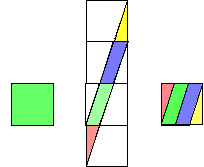
\includegraphics[width=\unitlength]{CatMapStatesp}}%
    \put(-0.025,0.15){\color[rgb]{0,0,0}\makebox(0,0)[lb]{\smash{$(0,0)$}}}%
    \put(0.26669086,0.17307744){\color[rgb]{0,0,0}\makebox(0,0)[lb]{\smash{B}}}%
    \put(0.26669086,0.41839762){\color[rgb]{0,0,0}\makebox(0,0)[lb]{\smash{C}}}%
    \put(0.02137069,0.41839762){\color[rgb]{0,0,0}\makebox(0,0)[lb]{\smash{D}}}%
    \put(0.38935094,0.00135332){\color[rgb]{0,0,0}\makebox(0,0)[lb]{\smash{B}}}%
    %\put(0.32,0.17){\color[rgb]{0,0,0}\makebox(0,0)[lb]{\smash{$(0,0)$}}}%
    \put(0.64284833,0.60647641){\color[rgb]{0,0,0}\makebox(0,0)[lb]{\smash{C}}}%
    \put(0.64284833,0.79455521){\color[rgb]{0,0,0}\makebox(0,0)[lb]{\smash{D}}}%
    %\put(0.79004043,0.42657495){\color[rgb]{0,0,0}\makebox(0,0)[lb]{\smash{A}}}%
    %\put(0.79004043,0.17307744){\color[rgb]{0,0,0}\makebox(0,0)[lb]{\smash{B}}}%
    %\put(0.96994189,0.17307744){\color[rgb]{0,0,0}\makebox(0,0)[lb]{\smash{C}}}%
    %\put(0.97811923,0.42657495){\color[rgb]{0,0,0}\makebox(0,0)[lb]{\smash{D}}}%
    \put(0.02,0.27){\color[rgb]{0,0,0}\rotatebox{90.0}{\makebox(0,0)[lb]{\smash{$\ssp_{0}$}}}}%
    \put(0.39,0.27){\color[rgb]{0,0,0}\rotatebox{90.0}{\makebox(0,0)[lb]{\smash{$\ssp_{1}$}}}}%
    \put(0.76,0.27){\color[rgb]{0,0,0}\rotatebox{90.0}{\makebox(0,0)[lb]{\smash{$\ssp_{1}$}}}}%
    \put(0.1469525,0.173){\color[rgb]{0,0,0}\makebox(0,0)[lb]{\smash{$\ssp_{-1}$}}}%
    \put(0.51493279,0.174){\color[rgb]{0,0,0}\makebox(0,0)[lb]{\smash{$\ssp_{0}$}}}%
    \put(0.86655824,0.175){\color[rgb]{0,0,0}\makebox(0,0)[lb]{\smash{$\ssp_{0}$}}}%
    \put(0.21762677,0.55482852){\color[rgb]{0,0,0}\rotatebox{43.35476392}{\makebox(0,0)[lb]{\smash{stretch}}}}%
    \put(0.74915379,0.61465381){\color[rgb]{0,0,0}\rotatebox{-46.94301089}{\makebox(0,0)[lb]{\smash{wrap}}}}%
  \end{picture}%
\end{center}
   \caption{ \label{fig:CatMapStatesp}
(Color online)
The Newtonian $s=3$  Arnol'd cat map matrix $A'$ \refeq{eq:StateSpCatMap}
keeps the origin $(0,0)$ fixed, but otherwise stretches the unit square
into a parallelogram. Translations by $\Ssym{0}$ from alphabet
$\A=\{\underline{1},0,1,2\}=$
\{%
{\color{red}red},
{\color{green}green},
{\color{blue}blue},
{\color{yellow}yellow}%
\}
bring stray regions back onto the torus.
   }
 \end{figure}
%%%%%%%%%%%%%%%%%%%%%%%%%%%%%%%%%%%%%%%%%%%%%%%%%%%%%%%%%%%%%%%%

\subsection{Percival-Vivaldi linear encoding partition of the \statesp}
\label{sect:catLinPartit}

To interpret $\Ssym{t}$'s, consider the action of
the Newtonian cat map \refeq{OneCat} on a 2\dmn\ \statesp\ point
$(\ssp_{t-1},\ssp_{t})$,
\beq
 \left(\begin{array}{c}
 \ssp_{t}  \\
 \ssp_{t+1}
 \end{array} \right )=
 A' \left(\begin{array}{c}
 \ssp_{t-1}  \\
 \ssp_{t}
 \end{array} \right ) %\mbox{ mod } 1
 - \left(\begin{array}{c}
 0  \\
 \Ssym{t}
 \end{array} \right )
 \,,  \qquad
 {A'} =\left(\begin{array}{cc}
 0 & 1 \\
 -1 & s
 \end{array} \right)
\,.
\ee{eq:StateSpCatMap}
In Percival and Vivaldi\rf{PerViv}, this representation of cat map is
referred to as ``the two-configuration representation''.
As illustrated in
\reffig{fig:CatMapStatesp}, in one time step the area preserving
map $A'$ stretches the unit square into a parallelogram, and a
point $(\ssp_{0},\ssp_{1})$ within the initial unit square
in general lands outside it, in another unit square $\Ssym{t}$
steps away. As they shepherd such stray points back into the unit
torus, the integers $\Ssym{t}$ can be interpreted as ``winding
numbers''\rf{Keating91}, or ``stabilising impulses''\rf{PerViv}.
The $\Ssym{t}$ translations reshuffle the \statesp, thus partitioning it into
$|\A|$ regions $\pS_\Ssym{}$, $\Ssym{}\in\A$.

As illustrated by \reffig{fig:CatMapStatesp}, there are the two kinds of
pieces within the state  space partition: the parallelograms
$\pS_0,\dots,\pS_{s-2}$, and the two exterior half sized  triangles
$\pS_{\underline{1}}$, $\pS_{s-1}$, labeled by the $(s\!-\!1)$-letter
\emph{interior} alphabet $\Ai$, and the two-letter \emph{exterior}
alphabet $\Ae$, respectively. For integer $s\geq2$ these alphabets are
\beq
\A=\Ai\cup\Ae
    \,,\qquad
\Ai=\{0, \cdots, s\!-\!2\}
    \,,\qquad
\Ae=\{\underline{1}, s\!-\!1\}
\,.
\ee{1dCatAlphs}

Refinements of these partitions work very much like they do for the
baker's map and the Smale horseshoe, by peering further into the future
and the past, and constructing the intersections of the future and past
partitions\rf{DasBuch}. The ``$\ell$-th level'' of partition $\pS = \cup
\pS_b$ is labeled by the set of all {\admissible} {\brick s} $b$ of length
$\ell$, composed of the past $\ell-t-1$ steps, and future $t$ steps, with
`decimal point' denoting the present,
\[
b  =
 \Ssym{t-\ell+1}\cdots\Ssym{-1}\Ssym{0}.\Ssym{1}\Ssym{2}\cdots\Ssym{t}
\,.
\]
    \edit{
For the cat map symbol \brick s $\Mm_{\R}$ is 1\dmn, and a domain \R\
consists of $\ell$ consecutive temporal lattice sites, so in this section
we shall denote $\Mm_{\R}$ by a \brick\ $b$ of length $\ell$, and refer to
the infinite length symbol \brick\ as `itinerary'.
    }

While an {\admissible} infinite itinerary defines a unique point in the
\statesp, a finite {\brick} $b$ determines
a \emph{cylinder set}
$\pS_b$, the set of all points
in $(x_0,x_1)$ plane having itineraries of the form
\[
\cdots a_{t-\ell-1} a_{t-\ell}\Ssym{t-\ell+1}\cdots\Ssym{-1}\Ssym{0}
.
\Ssym{1}\Ssym{2}\cdots\Ssym{t} a_{t+1}a_{t+2}\cdots
\,,
\]
with fixed $\Ssym{i}$'s, and arbitrary $a_{i}\in\A$.
How these {\brick s} partition the \statesp\ is best understood by
inspecting \reffig{fig:SingleCatPartit}.

%%%%%%%%%%%%%%%%%%%%%%%%%%%%%%%%%%%%%%%%%%%%%%%%%%%%%%%%%%%%%%%%%%
\begin{figure}
	\centering
	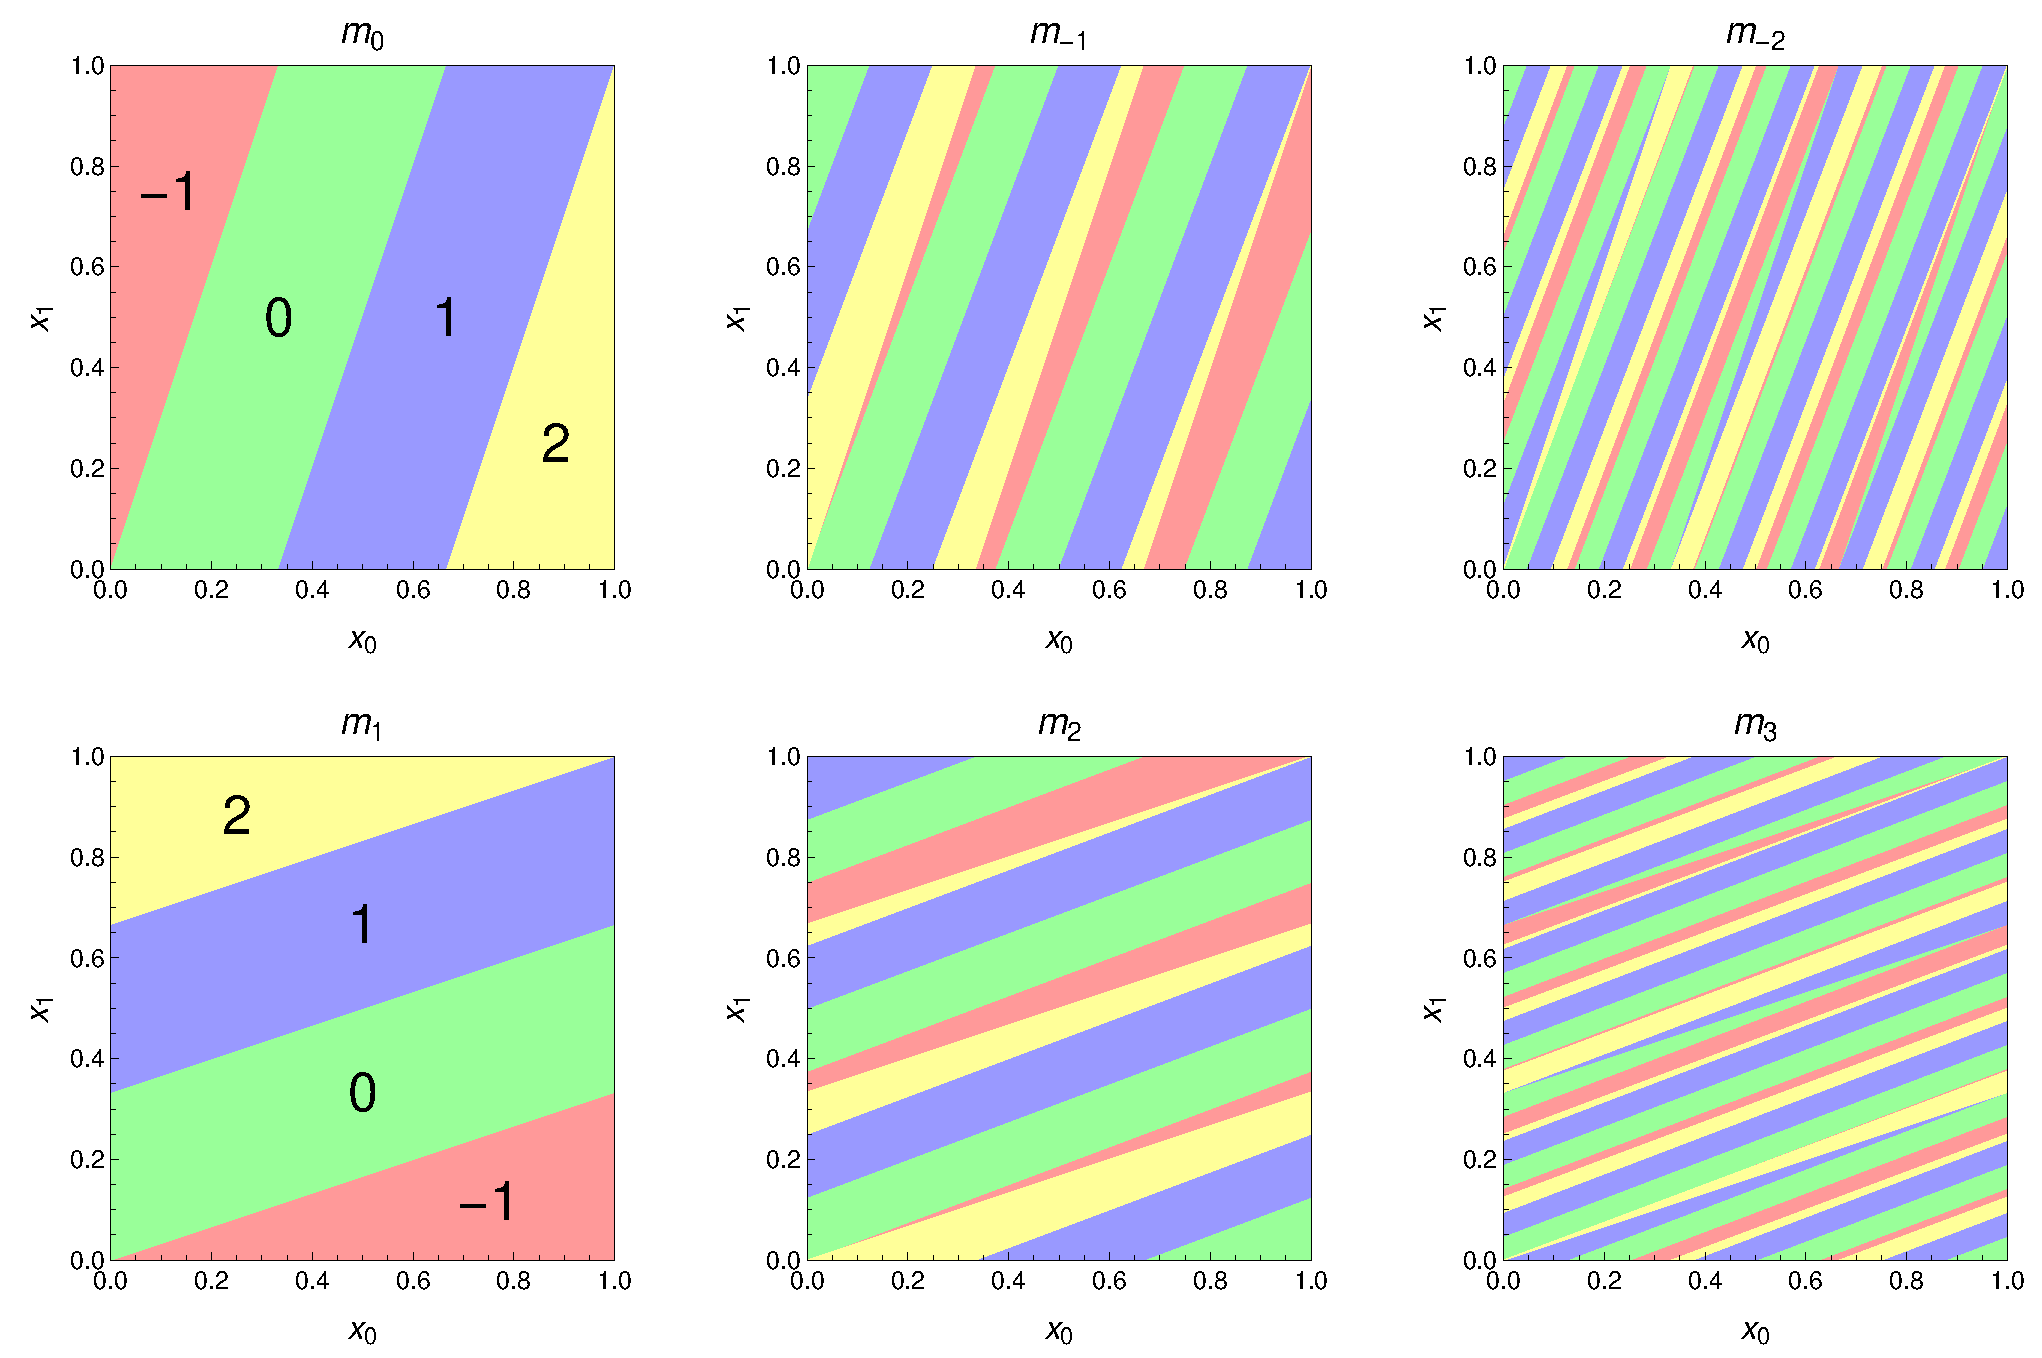
\includegraphics[width=0.95\textwidth]{SingleCat1Symbol}
\\
	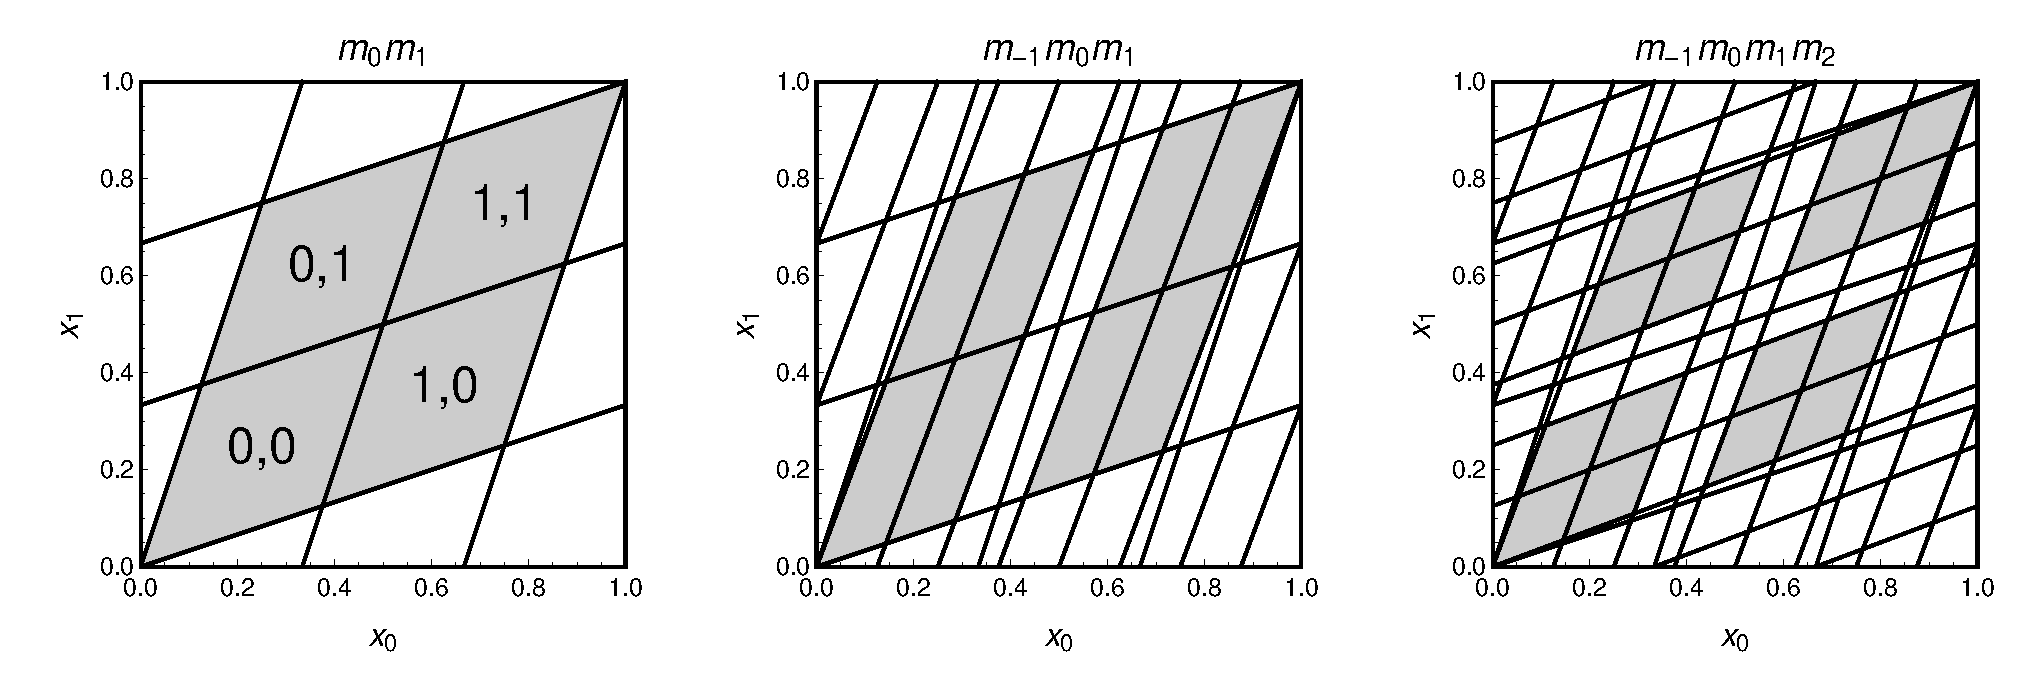
\includegraphics[width=0.97\textwidth]{SingleCatMultiSymbol}
	\caption{\label{fig:SingleCatPartit}
(Color online)
% Newtonian
Arnol'd cat map $(\ssp_{0},\ssp_{1})$  \statesp\ partition into
(a) 4 regions labeled by $\Ssym{0}.$ , obtained from
$(\ssp_{-1},\ssp_{0})$ \statesp\ by one iteration (the same as
\reffig{fig:CatMapStatesp}).
(b) 14 regions labeled by past {\brick} $\Ssym{-1}\Ssym{0}.$, obtained from
$(\ssp_{-2},\ssp_{-1})$ \statesp\ by two iterations.
(c) 44 regions, past {\brick} $\Ssym{-2}\Ssym{-1}\Ssym{0}.$
(d) 4 regions labeled by $.\Ssym{1}$ , obtained from
$(\ssp_{2},\ssp_{1})$ \statesp\ by one backward iteration.
(e) 14 regions labeled by future {\brick} $.\Ssym{1}\Ssym{2}$ , obtained from
$(\ssp_{3},\ssp_{2})$ \statesp\ by two backward iterations.
(f) 44 regions, future {\brick} $\Ssym{3}\Ssym{2}\Ssym{1}.$
Each color has the same total area ($1/6$ for $\Ssym{t} = \underline{1},
2$, and $1/3$ for $\Ssym{t} = 0, 1$).
\Statesp\ partition into
(g) 14 regions labeled by {\brick} $b = \Ssym{0}.\Ssym{1}$, the
intersection of one past (a) and
one future iteration (d).
(h) {\brick} $b = \Ssym{-1}\Ssym{0}.\Ssym{1}$, the intersection of two
past (b) and one future iteration (d).
(i) {\brick} $b = \Ssym{-1}\Ssym{0}.\Ssym{1}\Ssym{2}$, the intersection
of two past (b) and two future iterations (e).
Note that while some regions involving external alphabet (such as
\prune{22} in (g)) are pruned, the interior alphabet labels a horseshoe,
indicated by the shaded regions.
The first three covers of the horseshoe have areas (g) $4 \times
1/8$, (h) $8 \times 1/21$, and (i) $16 \times 1/55$.
All boundaries are straight lines with rational slopes.
	}
\end{figure}
%%%%%%%%%%%%%%%%%%%%%%%%%%%%%%%%%%%%%%%%%%%%%%%%%%%%%%%%%%%%%%%%%%


%%%%%%%%%%%%%%%%%%%%%%%%%%%%%%%%%%%%%%%%%%%%%%%%%%%%%%%%%%%%%
 \begin{table}
\begin{center}
\begin{tabular}{ c|cccc }
 & \underline{1} & 0 & 1 & 2\\
  \hline
 \underline{1} &  0  & 0.0208 &  0.0625 &  0.0833\\
 0 &  0.0208 &  0.1250 &  0.1250 &  0.0625 \\
 1 & 0.0625 & 0.1250 & 0.1250 &  0.0208\\
 2 & 0.0833 & 0.0625 &  0.0208&  0\\
\end{tabular}
%\approx
\quad
\begin{tabular}{ c|cccc }
 & \underline{1} & 0 & 1 & 2\\
  \hline
 \underline{1} &  0    & 1/48 &  1/16 &  1/12\\
 0 &  1/48 &  1/8 &  1/8 &  1/16 \\
  1 &  1/16 & 1/8  &  1/8 &  1/48\\
  2 & 1 /12 & 1/16 &  1/48 &  0\\
\end{tabular}
\end{center}
  \caption{\label{tab:RJ2letFreq}
The measures $\Msr(\Ssym{i}\Ssym{i+1})$ of the 16 distinct 2-symbol \brick s
$\Ssym{i} \Ssym{i+1}$ for the  $s=3$ Arnol'd cat map,
    (left)
obtained from a long-time ($\sim10^9$ iterations) numerical simulation
rounded off to  four significant  digits;
    (right)
the exact values given by \refeq{PairsFreq}, or read off as sub-partition
areas in \reffig{fig:SingleCatPartit}\,(g).
Column: \ $\Ssym{i}$.  Row: \ $\Ssym{i+1}$.
See \reffig{fig:SingleCatPartit} for a geometric picture of why {\brick
s}  $\underline{1}\underline{1}$ and $22$ are pruned.
  }
\end{table}
%%%%%%%%%%%%%%%%%%%%%%%%%%%%%%%%%%%%%%%%%%%%%%%%%%%%%%%%%%%%%


\subsection{From itineraries to orbits and back}
\label{sect:catLinGreen}

The power of the linear encoding for a cat map\rf{PerViv} is that one can
use  integers $\Ssym{t}$ to encode its \statesp\ trajectories. Since the
connection \refeq{OneCat}  between  sequences of $\Ssym{t}$ and
$\ssp_{t}$ is linear, it is straightforward  to go back and forth between
\statesp\ and symbolic representation of an orbit. In particular, if \(
\{\Ssym{t}\} \) is an {\admissible} itinerary, the corresponding
\statesp\ point  at the  $t$ time instant is given by the inverse of
\refeq{OneCat},
\beq
  \ssp_{t}=\sum_{t'=-\infty}^\infty \gd_{tt'} \Ssym{t'}
  \,, \qquad
  \gd_{tt'} =
       \left(\frac{1}{-\Box -2 +s}\right)_{tt'}
 \,.
\ee{Coord}
The matrix $\gd_{tt'}$ is the  Green's function for 1\dmn\
discretized heat equation\rf{PerViv,varcyc} given explicitly by
$\gd_{tt'}=\ExpaEig^{-|t-t'|}/(\ExpaEig-\ExpaEig^{-1})$,
$s=\ExpaEig+\ExpaEig^{-1}$, see \refeq{StabMtlpr} and \refappe{sect:Green}.

Although the recovery  of \statesp\ \po s from finite symbol \brick s is
straightforward for the linear encoding, it is not easy to
describe the grammar rules for which symbol \brick s are
{\admissible}\rf{PerViv87b}. For the linear encoding presented
here, there is no finite set of short pruned {\brick} grammar rules, in
contrast to linear encoding for the Adler--Weiss Markov \edit{generating}
partition of the  cat map \statesp\ given in \refref{DasBuch}. An
itinerary $\dots \Ssym{-1}\Ssym{0}\Ssym{1}\dots$  is {\admissible} if and
only if each  of the corresponding \statesp\ orbit points $\ssp_t$ in
\refeq{Coord} is in the unit interval $[0,1)$. Therefore, there is an
infinite number of conditions to satisfy. All  these conditions, however,
are automatically satisfied if the symbols $\Ssym{t}$ belong to the
interior alphabet  $\Ai$ \refeq{1dCatAlphs}. Indeed, if
$0\leq\Ssym{t}\leq s\!-\!2$ for all $t$, then
\beq
0\leq \sum_{t=-\infty}^{\infty}
      \frac{\Ssym{t}\ExpaEig^{-|t|}}{\ExpaEig-\ExpaEig^{-1}}
 \leq  \sum_{t=-\infty}^{\infty}
      \frac{(\ExpaEig^{-1}+\ExpaEig-2) \ExpaEig^{-|t|}}{\ExpaEig-\ExpaEig^{-1}}
 =1
 \,,
\ee{innerShift}
and  all  $\ssp_{t}$  generated by \refeq{Coord} fall into $[0,1)$.
As a result,  the interior part of the lattice states,  $\Ai^\integers$ is
a full shift,  with any infinite sequence of $\Ssym{t}\in\Ai$ being
{\admissible}. All grammar rules (``pruning'' of {\admissible} \brick s)
necessarily involve symbols from the {exterior} alphabet $\Ae$.


\subsection{Measures of cylinder sets}
\label{sect:catMfreq}

\subsubsection{Numerics.}

The \statesp\ coordinates $(\ssp_{0},\ssp_{1})$ are, up to the linear
shift $p_t = \ssp_{t} - \ssp_{t-1} \to \ssp_{t}$, equivalent to the
Hamiltonian $(\ssp_{0},p_{0})$ \edit{phase space coordinates}, and as the cat map is
invertible, ergodic, and area preserving, with the invariant measure
$\dMsr=dx_t dp_t=d\ssp_{t}\,d\ssp_{t-1}$ and uniform invariant density
$\rho(\ssp_0, \ssp_1) = 1$, the measure $\Msr({b})$ corresponding to a
{\brick} $b$ %=\Ssym{1}\Ssym{2}\cdots \Ssym{\ell}$
equals to the  area $|\pS_b|$ of a {\statesp} region $\pS_b$.
The $(\ssp_{0},\ssp_{1})$  \statesp\ is composed of a disjoint union of
regions $\pS = \cup \pS_b$ labelled by all
{\admissible} {\brick s} of a fixed length $|{b}|=\ell$, so the sum of all
measures $\Msr(b)$ equals the total area of the \statesp\ $|\pS|=1$,
\beq
   \sum_{|{b}|=\ell} \Msr({{b}})=1
  \,.
\ee{totMeasure} Area sums over
subpartitions, such as
\bea
 \sum_{\Ssym{1}} \Msr(\Ssym{1} \Ssym{2} \cdots \Ssym{\ell})
     &=& \Msr(\Ssym{2} \cdots \Ssym{\ell})
\continue
 \sum_{\Ssym{\ell}} \Msr(\Ssym{1} \Ssym{2} \cdots \Ssym{\ell})
     &=& \Msr(\Ssym{1} \cdots \Ssym{\ell-1})
     \,,
\label{MarginalFreq}
\eea
provide consistency checks for  computations.

By the ergodic  theorem, the relative frequency of  appearances of a
{\brick} ${b}$ in a generic ergodic trajectory equals $\Msr(b)$. This
allows for numerical estimates of $\Msr(b)$ by long ergodic
trajectories, as illustrated in \reftab{tab:RJ2letFreq}. For the problem
at hand, there is, in principle,  no need for such simulations, as the
areas $|\pS_{b}|$ of partitions for short \brick s $b$ can be evaluated
exactly using, for example, Mathematica geometric computation
tools\rf{Mathematica}. We have computed such tables for partitions up to
\brick\ length $|{b}|=12$, but the results are quickly too unwieldy and
unilluminating to tabulate here. We visualize instead the measures by
their areas in the $(\ssp_{0},\ssp_{1})$ plane, as illustrated in
\reffig{fig:SingleCatPartit}.

\subsubsection{Analytics.}

The number of $\pS_{b}$   grows exponentially with $|b|$, while  their
areas  $|\pS_{b}|$  shrink exponentially.
Furthermore, for  larger $|b|$, the domains $\pS_{b}$  split into
disjoint sets, making  it hard to determine their areas and the pruning
rules for longer \brick s.
Because of this, for the analytical  calculation of measures $\Msr(b)$,
the Lagrangian reformulation of the problem, with  fixed
boundary points $ \ssp_0$,  $\ssp_{\ell+1}$, turns out to be  more
powerful. Moreover, as we show in \refsect{sect:CCMmeasBrick},  the
Lagrangian formulation generalizes  in a natural way to the \catlatt\ in
any spatial dimension.


Let $\{\ssp_t\}$ be   a trajectory  generated by the cat map
and let  $\{\Ssym{t}\} $ be its symbolic  representation.
As we show in
\refappe{sect:Green}, the state $\ssp_t$ at time
$t\in \{1,\dots \ell\}$ can be
expressed through the {\brick}  ${b}=\Ssym{1}\Ssym{2}\dots
\Ssym{\ell}$ at the times  $1,\dots \ell$, and  the boundary
coordinates $(\ssp_0, \ssp_{\ell+1})$:
\beq
  \ssp_t=\sum_{t'=1}^{\ell} \gd_{tt'}\Ssym{t'}
          +\gd_{t1}\ssp_0+\gd_{t\ell}\ssp_{\ell+1}
  \,, \qquad t=1,\dots \ell,
\ee{inverseq}
where  $\gd$ is  the discrete Green's function  with the Dirichlet boundary
conditions at $t=0$ and $t=\ell+1$.

Explicitly,  $\gd_{tt'}$ can be expressed in terms of Chebyshev
polynomials of the second kind
$U_n(s/2)={\sinh[(n+1)\Lyap]}/{\sinh \Lyap}$:
\[
 \gd_{ij}= \left\{\begin{array}{lr}
        \frac{U_{i-1}(s/2)U_{\ell-j}(s/2)}{U_{\ell}(s/2)}, & \mbox{for } i\leq j\\
        \frac{U_{j-1}(s/2)U_{\ell-i}(s/2)}{U_{\ell}(s/2)}, & \mbox{for } i> j .
        \end{array}\right.
\]
The first term on the right hand side of  \refeq{inverseq},
\beq
  \bar{x}_i({b})=\sum_{j=1}^{\ell} \gd_{ij}\Ssym{j}
\,,
\ee{catMapAverCoord}
can be thought of as the ``approximate state'' at time $i$. Indeed, by
\refeq{inverseq} we have
\beq
 |\ssp_i-\bar{x}_i({b})|
 = \left|\frac{U_{\ell-i}(s/2)}{U_{\ell}(s/2)}\ssp_0
   + \frac{U_{i-1}(s/2)}{U_{\ell}(s/2)} \ssp_{\ell+1}\right|
   \leq \frac{\cosh (\frac{1}{2}(\ell+1)-i)\Lyap }{\cosh \frac{1}{2}(\ell+1)\Lyap}
\,.
\ee{error}
Hence the {\brick} ${b}$ determines  the lattice state at
the center
$i=\lfloor\ell/2\rfloor$  of the \brick\,  up to an exponentially small
error in $\ell$, of the order $e^{-\ell\Lyap/2}$.

\edit{
The following theorem allows  for evaluation of symbol \brick s measures.
\begin{theorem}\label{catTheorem}
Let $b$ be a finite \brick\ of $\ell$ symbols.  The corresponding
measure is given by the product
\beq
 \Msr({b}) =d_\ell |\Pol_{b}|,  \qquad  d_\ell =
  {1}/{U_{\ell}({s}/{2})},
\ee{FreqDecomp}
where
 $|\Pol_{b}|$ is  the area of the polygon $\Pol_{b}$
defined  by the inequalities
\begin{eqnarray}
 & 0&\leq \bar{x}_i({b})
     +\frac{U_{\ell-i}(s/2)}{U_{\ell}(s/2)}\ssp_0
     +\frac{U_{i-1}(s/2)}{U_{\ell}(s/2)} \ssp_{\ell+1}<1
     \,,\qquad i=1,\dots ,\ell,
\label{SquareCut1} \\
 & 0&\leq \ssp_0 <1, \qquad  0\leq \ssp_{\ell+1} <1
 \,
\label{SquareCut2}
\end{eqnarray}
in the plane $(\ssp_0,\ssp_{\ell+1})$.
\end{theorem}

\begin{proof}
From   \refeq{inverseq}  the element  $\pS_b$ of the partition $\pS$   is
defined  by the inequalities \refeq{SquareCut1} and \refeq{SquareCut2}.
 In general, the inequalities  (\ref{SquareCut1}) ''cut out''  a polygon $\Pol_{{b}}$ of the unit square (\ref{SquareCut2}) in the $(\ssp_0,\ssp_{\ell+1})$ plane.  As a
result, the measure of ${b}$ is  given by the product
\beq
 \Msr({b})=|\pS_b| =d_\ell |\Pol_{b}|
\ee{FreqDecomp1}
of  the area $|\Pol_{b}|$ of the polygon $\Pol_{b}$ and the Jacobian
$d_\ell$ of the transformation of the invariant phase space measure $\dMsr
=d\ssp_0 dp_0$ to the Lagrangian end points measure $d\ssp_0 d
\ssp_{\ell+1}$. Since the Jacobian  of the transformation from $(\ssp_0
,p_0)$ to $(\ssp_0,\ssp_1)$ equals $1$, the value of  $d_\ell$  can be
evaluated as  the Jacobian  of the transformation from $d\ssp_0 d\ssp_1$
to $d\ssp_0 d \ssp_{\ell+1}$. By \refeq{inverseq}, we therefore get
\bea
  d_\ell
= {|\partial (\ssp_0, \ssp_1)}/{\partial (\ssp_0, \ssp_{\ell+1})|}=\gd_{1\ell}  =
  {1}/{U_{\ell}({s}/{2})}
\,.
\label{SingleCatJacobian}
\eea
\end{proof}

For \brick s composed of interior symbols only  the theorem yields a simple corollary:

\begin{corollary}
If  $\Ssym{i}\in \Ai
\,, \quad  i=1,\dots |{b}|$.
The corresponding measure is given by
\[
\Msr({b})
= {1}/{U_{|{b}|}({s}/{2})}, \qquad  \Ssym{i}\in \Ai
\,, \quad  i=1,\dots |{b}|
\]
and depends  only  on the length of the \brick\ ${b}$.
\end{corollary}

\begin{proof}
If  all $\Ssym{i}$  belong to $ \Ai$, the inequalities
(\ref{SquareCut1})  are always satisfied, and  $\Pol_{{b}}$ are unit
squares of area $1$.  The proof then follows immediately   by eq.~\refeq{FreqDecomp}.
\end{proof}
} %end \edit

In general,   the area  $|\Pol_{{b}}|$ in \refeq{FreqDecomp}  depends on the
particular \brick\ $b$; the Jacobian $d_\ell$ is the same for all ${b}$'s
of length $\ell$.
The view from $(\ssp_0, \ssp_{\ell+1})$ state space has a natural
interpretation of area as the relative measure to \brick\ of all interior
symbols, \ie, the geometrical factor $|\Pol_{b}|$. In other words, as
illustrated by comparing \reffig{fig:SingleCatPartit} with
\reffig{fig:PairSymbol}, the Hamiltonian and the Lagrangian partition areas
are the same  up to the overall Jacobian factor $d_\ell$.
The power of the Lagrangian reformulation is now evident: in contrast to the
exponentially shrinking and disjoint (for sufficiently large $|b|$)  $\pS_b$
of \reffig{fig:SingleCatPartit}, $\Pol_{{b}}$ are always  simply connected
convex polygons cut out of the unit square, see \reffig{fig:PairSymbol}.

%%%%%%%%%%%%%%%%%%%%%%%%%%%%%%%%%%%%%%%%%%%%%%%%%%%%%%%%%%%%%
\begin{figure}
\begin{center}
(a) 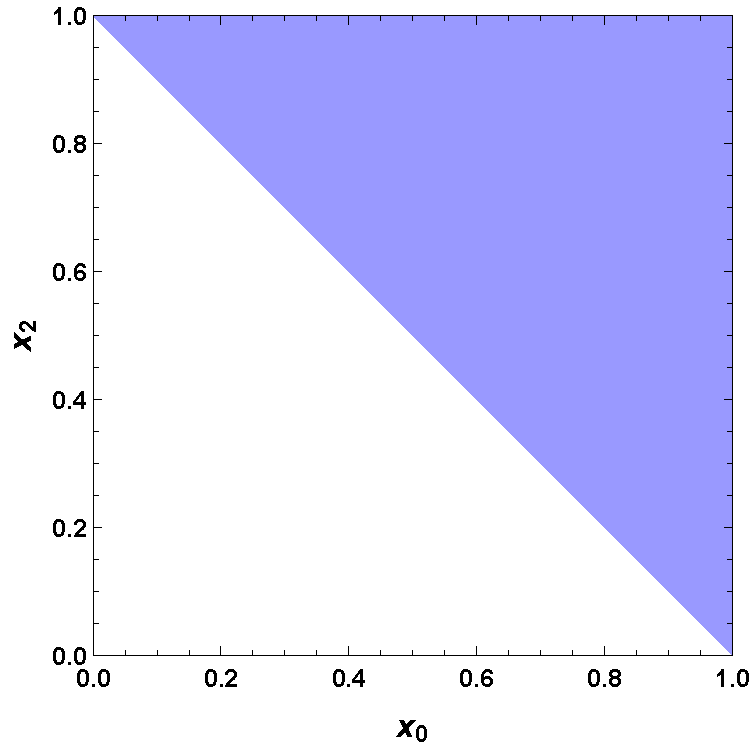
\includegraphics[height=0.29\textwidth]{BorisCatRegion1}
    \hspace{0.05\textwidth} 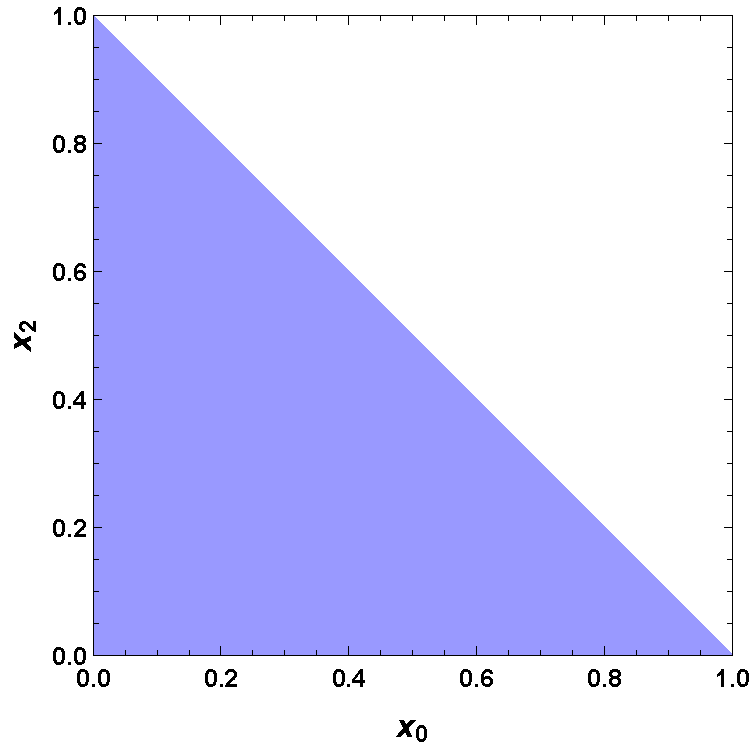
\includegraphics[height=0.29\textwidth]{BorisCatRegion2}
%(a)~~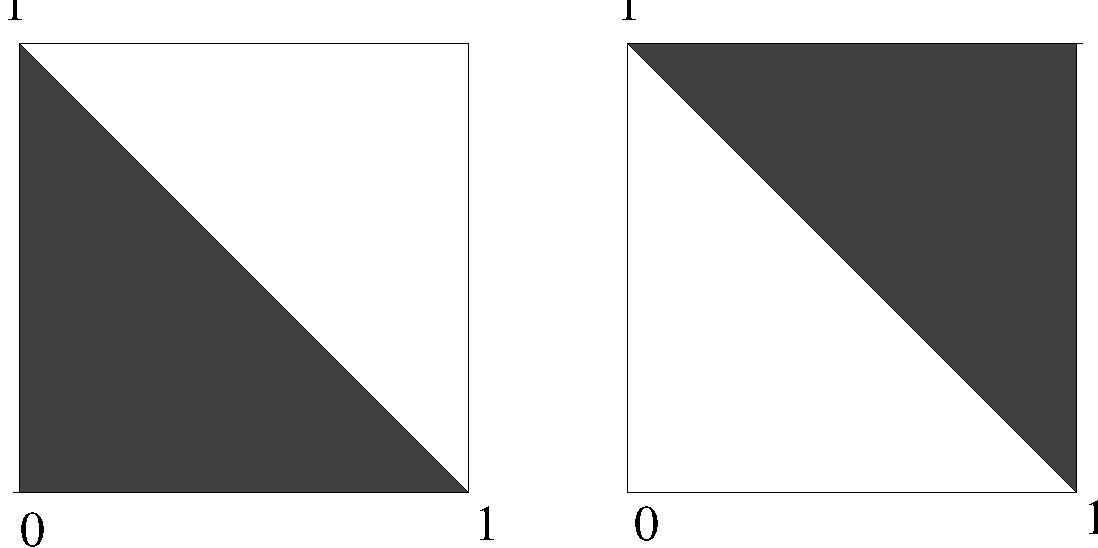
\includegraphics[height=0.27\textwidth]{SingleSymbol}

\medskip

(b) 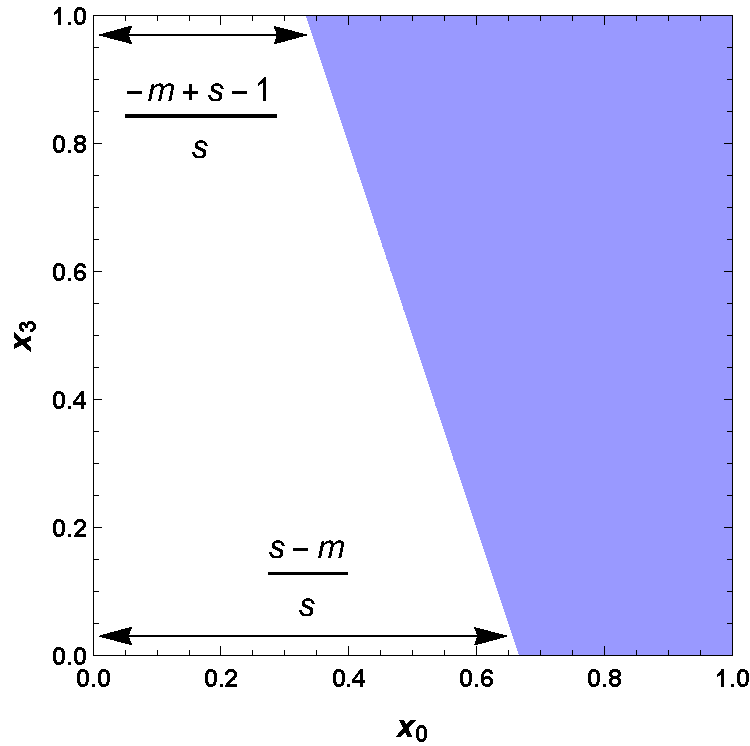
\includegraphics[height=0.29\textwidth]{BorisCatRegion4}
    \hspace{0.02\textwidth} 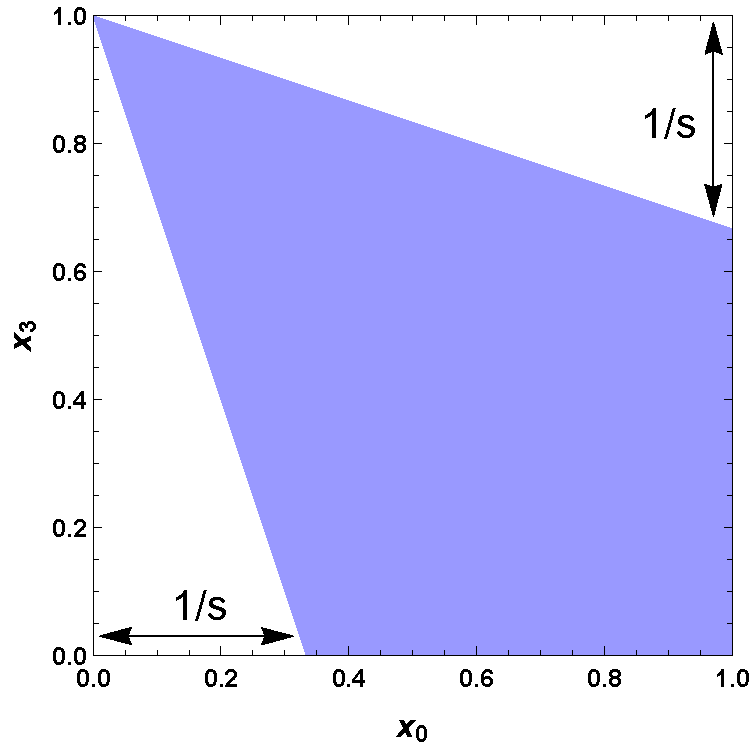
\includegraphics[height=0.29\textwidth]{BorisCatRegion3}
    \hspace{0.02\textwidth} 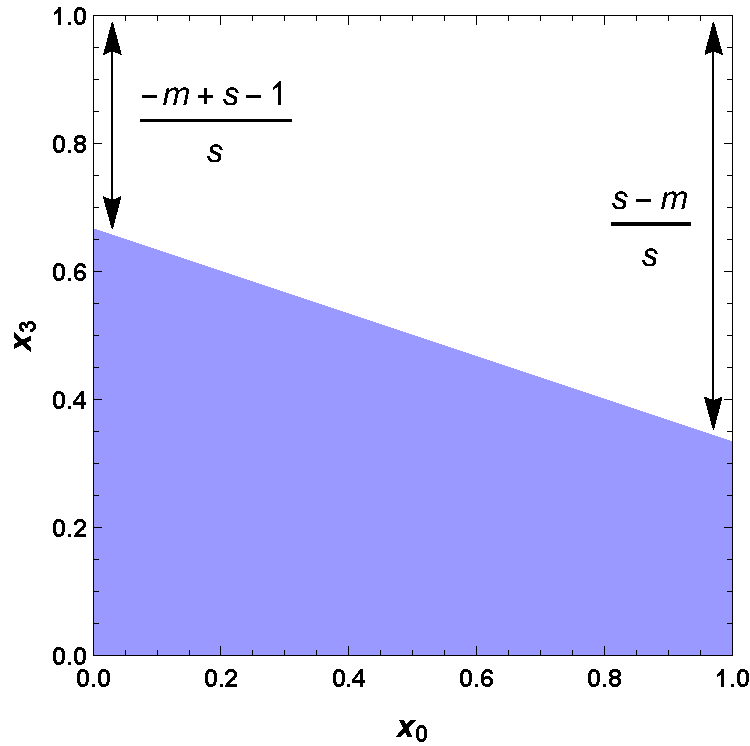
\includegraphics[height=0.29\textwidth]{BorisCatRegion5}
%(b)~~\includegraphics[height=0.27\textwidth]{PairSymbol}
\end{center}
\caption[]{\label{fig:PairSymbol}
(a) Polygons $\Pol_{m}$ (shaded areas)  for a single symbol,
     Lagrangian $(\ssp_0, \ssp_{2})$ plane, exterior letters $m\in \Ae$:
     (left)  $m=\underline{1}$,
     (right) $m=s\!-\!1$.
(b) Polygons $\Pol_{\Ssym{1} \Ssym{2}}$ (shaded areas) in Lagrangian
    $(\ssp_0, \ssp_{3})$ plane for {\brick s} $\block{\Ssym{1} \Ssym{2}}$
    of length 2,
    $\Ssym{1} =\underline{1},  \Ssym{2}= m\in \Ai$ (left);
    $\Ssym{1} =\underline{1},  \Ssym{2}=s-1$ (middle);
    $\Ssym{1} =s-1, \Ssym{2}=m \in \Ai$ (right).
Repeated exterior alphabet symbols are pruned,
$\Pol_{\Ssym{}\Ssym{}}= \emptyset$ if $\Ssym{}\in\Ae$.
For \brick s composed of only interior symbols $m_1,m_2\in \Ai$,  $\Pol_{\Ssym{1} \Ssym{2}}$ is the
entire unit square (full shift, no pruning).
Note that $\Msr({{b}})= \Msr({\bar{{b}}})$ by the symmetry \refeq{symmetry}.
Compare also with the \statesp\ representation \reffig{fig:SingleCatPartit}.
}
\end{figure}
%%%%%%%%%%%%%%%%%%%%%%%%%%%%%%%%%%%%%%%%%%%%%%%%%%%%%%%%%%%%%

\subsection{Evaluation of measures}
\label{sect:catFreqEval}


Since all coefficients in  (\ref{SquareCut1})  are given by rational
numbers, the polygon areas $|\Pol_{{b}}|$ are rational too. The same
holds for the $d_\ell$ factor. As a result,   measures  $\Msr({{b}})$ are
always rational (see, for example, \reftab{tab:RJ2letFreq}). This allows
for their exact evaluation by integer arithmetic.  As the factor $d_\ell$
in \refeq{FreqDecomp} is known explicitly, the evaluation   of
$\Msr({b})$ relies on the knowledge of the areas $|\Pol_{{b}}|$ which can
be easily found  analytically for small $\ell$. Before working out
specific examples, we list \edit{symmetry} properties of measures
$\Msr({b})$ valid for any \brick\ length $\ell$.

\paragraph{Symmetries.}
Symmetries of the cat map induce  invariance with respect to
corresponding symbol exchanges. Define $\bar{m}=s\!-\!2\!-\!m$ to be the
conjugate of symbol $m \in \A$. For example, the two exterior
alphabet \Ae\ symbols are conjugate to each other, as illustrated by
\reffig{fig:CatMapStatesp}.
If ${b}=\Ssym{1} \Ssym{2} \dots \Ssym{\ell}$ is a
\brick, and  $\bar{{b}}=\bar{m}_1 \bar{m}_2 \dots
\bar{m}_\ell$ its conjugate, then by  reflection symmetry of the cat
map we have  $|\Pol_{{b}}|= |\Pol_{\bar{{b}}}|$. Similarly, if
$b^*=\Ssym{l}\Ssym{l-1}\dots \Ssym{1}$, the time reversal invariance implies
$|\Pol_{{b}}|=|\Pol_{{b}^*}|$. Accordingly,
\brick s $ {b}$, $ {b}^*$, and $\bar{{b}}$ have the same
measure,
 \beq
 \Msr({{b}})= \Msr({\bar{{b}}})=\Msr({{b}^*})
 \,.
 \ee{symmetry}



\subsubsection{Example: Measure of \brick s of length $\ell=1$.}

The defining, single symbol \brick\ Lagrangian equation
\refeq{eq:CatMapNewton1} is the simplest example of the Lagrangian,
two-point boundary values formulation,
\[
  \ssp_1=\gd_{11}\Ssym{1}
          +\gd_{11}\ssp_0+\gd_{11}\ssp_{2}
\,,
\]
with $\ell=1$,  $\gd_{11}=1/s$
verifying the general Green's function formula \refeq{inverseq}.
For  single symbol $\Ssym{1}\equiv m$ the set of inequalities
(\ref{SquareCut1}) thus reduces to
 \[
   -m \leq \ssp_{0}+\ssp_{2} < s-m
 \,.
\]
This constraint is always fulfilled for interior symbols $m\in \Ai$. For
$m\in \Ae$, polygon $\Pol_{m}$ is the upper and lower triangle, respectively,
shown in \reffig{fig:PairSymbol}\,(a).
As a result, we have   $|\Pol_{m}|=1$ if $m\in \Ai$ and $|\Pol_{m}|=1/2$
if $m\in \Ae$, giving measures
\[
 \Msr(m)= \left\{\begin{array}{ll}
       1/s, & \mbox{for } m\in \Ai \\
        1/2s, & \mbox{for } m\in \Ae \,,
        \end{array}\right.
\]
which indeed add up to
\edit{one after summation over all letters of the alphabet $\A$.}


 \subsubsection{Example: Measure of \brick s of length $\ell=2$:}
 \label{1Dblock2}

For {\brick s} $\Ssym{1} \Ssym{2}$, bounds (\ref{SquareCut1}) give four
inequalities
\bea
  -s\Ssym{1}-\Ssym{2} &\leq& s\ssp_{0}+\ssp_{3} < s^2-1 - s\Ssym{1}-\Ssym{2}\\
  -s\Ssym{2}-\Ssym{1} &\leq& s\ssp_{3}+\ssp_{0} < s^2-1 - s\Ssym{2}-\Ssym{1}
  \,,
  \nonumber
\eea
where we have used $U_2(s/2)=s^2-1$.
A constraint arises  whenever at least  one of the symbols belongs to
the exterior alphabet
\Ae. By the symmetry (\ref{symmetry}), it is sufficient to analyze the
case when $\Ssym{1}=\underline{1}$. If $\Ssym{2}\in
\Ai$, the \edit{polygon} $\Pol_{\underline{1}m_2}$ is determined by (see
\reffig{fig:PairSymbol}\,(b)):
 \[
  s-\Ssym{2}\leq s\ssp_{0}+\ssp_{3},   \qquad 0\leq \ssp_{0},\ssp_{3} <1.
 \]
The area of the  resulting polygon is equal  to   $|\Pol_{\underline{1}
m_2}|=(1+2m_2)/2s$, where   $m_2\in \Ai$.
If both $\Ssym{1} \neq \Ssym{2}$ belong to \Ae, i.e.,
$\Ssym{1}=\underline{1}$, $\Ssym{2}=s\!-\!1$, then the corresponding
polygon is determined by the conditions:
 \[
  1\leq s\ssp_{0}+\ssp_{3},   \qquad  s\ssp_{3}
        +\ssp_{0} \leq s,   \qquad 0\leq \ssp_{0},\ssp_{3} <1.
 \]
with the corresponding area  $|\Pol_{\Ssym{1} \Ssym{2}}|=1-1/s$. Finally,
if both  $\Ssym{1}=\Ssym{2}$ belong to \Ae\  and they are equal, then
\brick\ is pruned,
$\Pol_{\Ssym{1} \Ssym{2}}=\emptyset$; there are two pruned \brick s of
length 2. In summary,
\beq
 \Msr(\Ssym{1} \Ssym{2})= \left\{\begin{array}{llll}
       1/s^2-1 & \mbox{for } \Ssym{1}, \Ssym{2}\in \Ai \\
        (1+2\Ssym{2})/2s(s^2-1) & \mbox{for } \Ssym{1}=\underline{1}, \Ssym{2}\in \Ai\\
        1/s(s+1) & \mbox{for } \Ssym{1}=\underline{1}, \Ssym{2}=s\!-\!1\\
        0 & \mbox{for } \Ssym{1}=\underline{1}, \Ssym{2}=\underline{1}.
        \end{array}\right.
\ee{PairsFreq}
The measures for the remaining  symbol combinations  can be obtained by the
symmetries, see  \refeq{symmetry} and \reftab{tab:RJ2letFreq} for the $s=3$
case.

\subsubsection{Pruning.}
\label{sect:catPruning}

As shown in \refeq{innerShift}, any \brick\ of \Ai\ symbols is
{\admissible}. If, on the other hand, one or more symbols from $\Ssym{}$ belong
to \Ae, such a \brick\ might be forbidden, with the \edit{polygon} $\Pol_{\Ssym{}}$
defined  by (\ref{SquareCut1},\ref{SquareCut2}) empty, and thus $\Msr(\Ssym{})=0$.
An example is the pruned \brick s \prune{\underline{1}\underline{1}} and
\prune{22}, missing from \reffig{fig:SingleCatPartit}\,(g). While here we
do not attempt to solve the number-theoretic problem of determining the
number of pruned \brick s for arbitrary $\ell$, the count of pruning
rules given in \reftab{tab:RJpruning} indicates that for the linear {encoding}
the number of pruned \brick s grows exponentially with their length. Thus
the linear {encoding} is not a subshift of finite type, as  its grammar
consists of an infinity of arbitrarily long pruned (\ie, \edit{\inadmissible})
{\brick s}.
While the shaded areas of \reffig{fig:SingleCatPartit}\,(g-h) are
accounted for by the complete Smale-horseshoe grammar of the interior
alphabet, the admissibility  rules for  {\brick}s involving  letters
from $\Ae=\{\underline{1},2\}$  are not known.
In \refref{CL18}, an \edit{Adler--Weiss Markov \edit{generating}
partition} symbolic dynamics for the \PV\ cat map
\refeq{eq:StateSpCatMap} is constructed, with complete, finite subshift
grammar. That, however, has no bearing on  the main thrust of this paper.

%%%%%%%%%%%%%%%%%%%%%%%%%%%%%%%%%%%%%%%%%%%%%%%%%%%%%%%%%%%%%%%%%%%%%%%%
%           \begin{table}\begin{center}
\Table{\label{tab:RJpruning}   % Nonlinearity macro
%	\caption{\label{tab:RJpruning}
$N_n$ is the total number of pruned {\brick s} of length  $n=\cl{b}$ for
the $s=3$ Arnol'd cat map. $\tilde{N}_n$ is the number of \emph{new}
pruned {\brick s} of length  $\cl{b}$, with all length  $\cl{b}$ {\brick
s} that contain shorter pruned {\brick s} already eliminated. Empirically
there is a single new pruning rule for each prime-number \brick\ length (it is
listed as two rules, but by the reflection symmetry there is only one).
}
%            \begin{minipage}[t][][b]{0.33\textwidth}
\begin{tabular}{rrr} % Nonlinearity style, see nonlinTips.tex
\br
  % after \\: \hline or \cline{col1-col2} \cline{col3-col4} ...
  $n$ & $N_n$ & $\tilde{N}_{n-1}$ \\
\hline  %\mr
  2 & 2 & 0 \\
  3 & 22 & 2 \\
  4 & 132 & 8 \\
  5 & 684 & 2 \\
  6 & 3164 & 30 \\
  7 & 13894 & 2 \\
  8 & 58912 & 70 \\
  9 & 244678 & 16 \\
  10 & 1002558 & 198 \\
  11 & 4073528 & 2 \\
  12 & 16460290 & 528 \\
  13 &   & 2 \\
\br
\end{tabular}
%            \end{minipage}\end{center}\end{table}\br
\endTable
%%%%%%%%%%%%%%%%%%%%%%%%%%%%%%%%%%%%%%%%%%%%%%%%%%%%%%%%%%%%%%%%%%%%%%%%

\section{\catLatt}
\label{sect:CCMs}

We now turn to the study of the {\catlatt} \refeq{LinearConn}, with cat maps
on sites (``particles'') coupled isotropically to their nearest neighbors on
a 2\dmn\ {\spt}ly infinite $\integers^2$ lattice.
The coupled map lattices (CML) were introduced in the mid 1980's as
models\rf{Kaneko83,Kaneko84} for studies of spatio-temporal chaos in
discretizations of dissipative PDEs. Later on, chains of coupled Anosov
maps were investigated in mathematically rigorous
settings\rf{BunSin88,PesSin88}. The conventional CML models start out
with chaotic on-site dynamics weakly coupled to neighboring sites, with
strong spacetime asymmetry. In order to establish the desired
statistical properties of CML, such as the continuity of their {SRB}
measures, \refrefs{BunSin88,PesSin88} and most of the subsequent
mathematical literature rely on the structural stability of Anosov
automorphisms under small perturbations.
Contrast this with the non-perturbative $2$\dmn\ \GO\rf{GutOsi15}
{\em \catlatt} \refeq{LinearConn}.
While this model has a Hamiltonian formulation (see
\refappe{sect:HamiltonCatLatt}), as in the {cat map} case of
\refsect{sect:catLinSymDyn}, it is instructive to write down its
equations of motion in the Lagrangian form:
\bea
 (-\Box +\edit{2(s-2)})\,\ssp_{z} &=& \Ssym{z}
\,,\qquad
 z=(n,t)\in \integers^{2}
\,,
\continue
  \ssp_{z}\in [0,1), \quad  && \Ssym{z}\in \A
  = \{-3, -2,\cdots,\edit{2s}-2,\edit{2s}-1\}
\,,
\label{CoupledCats}
\eea
with $\Box $ being the discrete spacetime Laplacian \refeq{LaplSpaceTime}
on $\integers^2$. The map is space $\leftrightarrow$ time symmetric and
has the temporal and spatial dynamics strongly coupled. Furthermore, it is
smooth and fully hyperbolic for any integer $|s|>\edit{2}$. In what follows we
will assume positive $s>\edit{2}$.

In this paper, we focus on learning how to enumerate
{\admissible} \catlatt\ {\spt} patterns, compute their measures, and identify
their recurrences (shadowing of a large \twot\ by smaller \twots).


\subsection{Linear encoding}
\label{sect:CCMlinSymDyn}

The symbols $\Ssym{z}$ from the set
$\A=\{\underline{3},\underline{2}, \cdots,\edit{2s}\!-\!2, \edit{2s}\!-\!1\}$
on the right hand side of \refeq{CoupledCats} are necessary to keep
$\ssp_{z}$ within the interval $[0,1)$, with \edit{$\underline{m_z}$}
standing here for $m_z$ with the negative sign, \ie, `$\underline{3}$'
stands for symbol `$-3$'. As we now show,
\(
\edit{
\Mm= \{\Ssym{z} \in \A \,,\; z\in \integers^2 \}
     }
\)
can be used as a 2\dmn\ symbolic representation (code) of the
lattice system states.

Since \refeq{CoupledCats} is a linear equation, any of its solutions
\(\Xx= \{x_{z} \in [0,1) \,,\; z\in \integers^2 \}\) can be
uniquely recovered from the corresponding code \Mm.
By inverting \refeq{CoupledCats} we obtain
\begin{equation}
  \ssp_{z}=\sum_{z'\in\integers^2}\gd_{z z'} \Ssym{z'}, \qquad  \gd_{z z' }
       =\left(\frac{1}{-\Box +\edit{2(s-2)}}\right)_{zz'}
       \,,
\label{GreenFuncCoupled}
 \end{equation}
where $\gd_{z z'}$ is the Green's function for the 2\dmn\ discretized heat
equation, see \refappe{sect:Green}. A symbol \brick\ $\Mm$ is
{\admissible} if and only if all $\ssp_{z}$ given by
\refeq{GreenFuncCoupled} fall into the interval $[0,1)$.

As for the {cat map}, we split the $\edit{2s}+3$ letter alphabet $\A=\Ai\cup\Ae$
into the interior \Ai\ and exterior \Ae\ alphabets
\beq
  \Ai=\{0,\dots,\edit{2({s}-2)}\},   \quad
  \Ae=
\{\underline{3},\underline{2},\underline{1}\}\cup
\{\edit{2s}\!-\!3,\edit{2s}\!-\!2,\edit{2s}\!-\!1\}
\,.
\ee{2dCatLattAlph}
For example, for $s=\edit{5/2}$ the interior, respectively exterior alphabets are
\beq
  \Ai=\{0,1\},   \quad
  \Ae=\{\underline{3},\underline{2},\underline{1}\}\cup \{2,3,4\}
\,.
\ee{2dCatLattAlph5}
If all $\Ssym{z}\in \Mm$ belong to \Ai, $\Mm$ is
{\admissible}, i.e., $\Ai^{\integers^2}$ is a full shift.
Indeed, by the positivity of Green's function (see \refappe{sect:Green})
it follows immediately that $0 \leq \ssp_{z}$, while the condition
$\sum_{z'\in \Zz}\gd_{zz'}=\edit{1/2({s}-2)}$ implies that $\ssp_z\leq 1$,
with the equality saturated only if $\Ssym{z}=\edit{2({s}-2)}$, for all
$z\in \Zz$.

The key advantage of linear encoding is illustrated already by the $d=2$
case. While the size of the alphabet \Aa\ based on a Markov partition
grows exponentially with the ``particle number'' $L$, the number of
letters \refeq{LinearConn} of the linear encoding \A\ is finite and the same
for any $L$, including the $L\to\infty$ \catlatt. For the linear encoding an
\twot\ is encoded by a doubly periodic $d=2$ {\brick} $\Mm$ of symbols
from a small alphabet, rather then by a $1$\dmn\ temporal string of
symbols from the exponentially large (in $L$) alphabet \Aa.


\subsection{Finite symbol \brick s}
\label{sect:CCMmeasBrick}

Let $\R\subset\Zz$ be a \edit{rectangle} on $\Zz$ and
let $\MmR=\{\Ssym{z}| z\in \R\}$ be a symbol \brick\ defined on \R. We
now show that $\MmR$ determines approximate positions of the points
$\ssp_z$, $z\in\R$, within the domain \R. To start with we define the
(exterior) boundary $\partial\R$ of $\R$ as a set of points adjacent to
$\R$. More precisely, $z=(n,t)$ belongs to $\partial\R$ if and only if
$z\notin \R$ but one of the four neighboring points $(n\pm 1,t)$, $(n,
t\pm 1)$ belongs to $\R$, see \reffig{fig:block2x2}(a). Let then
$\gd_{zz'}$ be the corresponding Dirichlet Green's function which
vanishes at the boundary $\partial\R$.
By the lattice Green's identity (see \refappe{sect:Green2Dident}) any
solution of the equation \refeq{CoupledCats} satisfies
\beq
 \ssp_z=\sum_{z'\in \R}\gd_{zz'} \Ssym{z'}
 + \sum_{z''\in\partial \R}\gd_{z\bar{z}''}\ssp_{z''}
 \,, \qquad  z\in \R
 \,,
\ee{DirichletGreenEquation}
with $\bar{z}''$ being the unique adjacent point of $z''\in \partial \R$
within the domain $\R$. Here, the first term
\beq
\bar{x}_z:= \sum_{z'\in \R}\gd_{zz'} \Ssym{z'}
\ee{BGaverCatLattPt}
can be viewed as the ``approximate {\spt} state''
$\bar{x}({\Mm_\R})$ at the point $z$. Importantly, it  is
determined solely by $\Mm_{\R}$. From \refeq{DirichletGreenEquation} it
follows that the difference $|\ssp_z -\bar{x}_z|$ is bounded by
\[
|\ssp_z -\bar{x}_z|
= \sum_{z''\in\partial \R}\gd_{z\bar{z}''}\ssp_{z''}
  \leq  |\partial \R|\,  \gd_{z\bar{z}''_{0}}
\,,
\]
with $\bar{z}''_{0}$ being the boundary point of $\R$
(\ie, adjacent to $\partial \R$), where the function $\gd_{z
\bar{z}''}$ attains its maximum value along $\partial \R$ (for a fixed
$z$).
\edit{
 For an illustration,
consider a $[\ell_1\!\times\!\ell_2]$ rectangular domain
\begin{equation}
\R^{[\ell_1\times\ell_2]}=
            \{(i, j)|\,i=0,\cdots,\ell_1\!-\!1,\;j=0,\cdots,\ell_2\!-\!1\}
\,,\label{Rectangular}
\end{equation}
with  $\ell_1$,  $\ell_2$ even (see \reffig{fig:block2x2}\,(a)),  and take
the point $z$ at  the rectangular center.
As the  Green's function
$\gd_{z\bar{z}''}$  decays exponentially with $|z-\bar{z}''|$
(see \ref{sect:Green2D}), the distance $|\ssp_z -\bar{x}_z|$ is  of the
order $e^{-\nu\ell_{\min}}$ for a large
$\ell_{\min}=\min{\{\ell_1/2,\ell_2/2\}}$, where the exponent
$\nu$ is defined by  $\cosh \nu =s/\edit{2}$.
} %end \edit

We determine next the measure $\Msr(\MmR)$ of the cylinder set
corresponding to $\MmR$. Take
\(
\R = \R^{[\ell_1\times\ell_2]}
\)
to be a  rectangular domain \refeq{Rectangular}. In what follows it is
convenient to distinguish   points in the interior of \R\  from the
points  which belong to the boundary $\partial \R$. While in principle
the boundary \statesp\ points $\ssp_{z''}\in\partial \R$ are labelled by
the symbol pair $z''=(n,t)$, we find it more convenient to label them by
a single index that indicates their position along the border, $\ssp_{i}
= \ssp_{z''}$, where $i$ runs from $1$ to
$\cl{\partial\R}=2(\ell_1+\ell_2)$. For examples, see
\reffig{fig:block2x2} and \refsects{exam:block1x1}{exam:block2x2}. Both
the boundary \statesp\ points $\ssp_i, i=1,\dots \cl{\partial \R}$ and
the internal points $\ssp_{z}, z\in\R$ must lie within the unit interval.

%%%%%%%%%%%%%%%%%%%%% GHJSC16_BG201113.tex start %%%%%%%%%%%%%%%%%%%%%%%%%
                      \edit{
\begin{theorem}\label{catLattTheorem}
Given a \brick\ of symbols $\MmR$ on \PCedit{rectangle} $\R$, the measure
$\Msr(\MmR)$ can be factorized into product
\beq
 \Msr(\MmR)=d(\R)\,|\Pol(\MmR)|
 \,,
\ee{CoupledFactorization}
where  $|\Pol(\MmR)|$ is the volume of the $\cl{\partial \R}$-dimensional
polytope $\Pol(\MmR)$, defined by the following inequalities
\begin{eqnarray}
& 0 & \leq  \ssp_{i}<1, \qquad i=1,\dots, \cl{\partial \R}
            \,,\label{polytop1}\\
& 0 & \leq  \bar{x}_z + \sum_{i=1}^\cl{\partial \R}
    \gd_{z\bar{z}_i}\ssp_{i}<1, \qquad z\in\R
\label{polytop}
\,
\end{eqnarray}
and   the factor $d(\R)$ depends only on the sizes $\ell_1,\ell_2$  of
\R, but not on the symbolic content of $\MmR$.
\end{theorem}

\begin{proof}
Since for all interior points $z\in \R$ one has  $0 \leq x_z<1$,
\refeq{DirichletGreenEquation} implies that  the {\admissible} set of
boundary points  $\ssp_i, i=1,\dots ,\cl{\partial \R}$  satisfy
inequalities \refeq{polytop1}  and \refeq{polytop}. Essentially, the
inequalities    \refeq{polytop}  cut   out the polytope $\Pol(\MmR)$ out
of the $\cl{\partial \R}$\dmn\ unit hypercube defined by
\refeq{polytop1}.  As a result, the measure    $\Msr(\MmR)$ is given by
the product of the  $\Pol(\MmR)$ volume and the Jacobian $d(\R)$ of
the linear transformation  between boundary  coordinates \refeq{polytop1}
and the  set  of $2(\ell_1+\ell_2)$  coordinates
\[
\{(x_{n  t_0}, x_{n t_1}) \, | \, n
 = -\lfloor\ell_2/2\rfloor,\dots ,-\lfloor\ell_2/2\rfloor+\ell_1+\ell_2-2\}
\]
at the  two  consecutive   times $t_0=\lfloor\ell_1/2\rfloor$, $t_1=t_0+1$.
Since  the Jacobian of this transformation is independent of any
particular \brick\ $\MmR$,  the
factor $d(\R)$ depends only on \R, but  not
on its symbolic content.
\end{proof}

As was the case for the single cat map theorem~\ref{catTheorem}, the
theorem yields  a simple result  for symbol  \brick s composed only
of the interior alphabet symbols:

\begin{corollary}
If all symbols in $\MmR$ belong to the interior alphabet \Ai\
\refeq{2dCatLattAlph}, then
\beq
  \Msr(\MmR)={d(\R)}
\ee{msrMmR}
is independent of the symbolic content of $\MmR$.
\end{corollary}

\begin{proof}
Note that the inequalities \refeq{polytop} are satisfied if all symbols
from $\MmR$ belong to the interior alphabet \Ai\
\refeq{2dCatLattAlph}. This follows from the positivity of the Green's
function $\gd_{zz'}$, and the identity
\[
  1 = 2(s-2)\sum_{z'\in \R}\gd_{zz'}
      + \sum_{z''\in\partial \R}\gd_{z\bar{z}''}, \qquad  z\in \R
\,,
\]
obtained by substituting the \catlatt\ \refeq{CoupledCats}  constant
field solution $\ssp_z=1$, $\Ssym{z}=2(s-2)$ into the Green's function
\refeq{DirichletGreenEquation} - see discussion following
\refeq{2dCatLattAlph5}.
As a result, for any {\brick} $\MmR$ of interior symbols   $\Pol({\MmR})$
is just a hypercube with   $|\Pol({\MmR})|=1$, and  \refeq{msrMmR}
follows immediately.
\end{proof}
    } %end \edit{
%%%%%%%%%%%%%%%%%%%%% GHJSC16_BG201113.tex end %%%%%%%%%%%%%%%%%%%%%%%%%

%%%%%%%%%%%%%%%%%%%%% GHJSC16_BG201113.tex start %%%%%%%%%%%%%%%%%%%%%%%%%
                      \edit{
\subsection{Evaluation of measures}
\label{sect:catLattFreqEval}

The evaluation of measures $\Msr(\MmR)$ for the \catlatt\   boils down to
the evaluation of  the polytope volumes $|\Pol({\MmR})|$, determined by
the inequalities \refeq{polytop1} and \refeq{polytop}. By the rationality
of every element $\gd_{zz'}$, $|\Pol({\MmR})|$ is given by a rational
number for any $\MmR$. This allows for  exact evaluation of
$|\Pol({\MmR})|$ by integer arithmetic. Once the volumes are found for
all {\admissible} \brick s $\MmR$, the constant factor $d(\R)$ can be
extracted from the normalization condition, by  summing up all volumes:
\beq
 1/d(\R) = \sum|\Pol({\MmR})|
\,.
\ee{CoupledPrefactor}
We were unable to derive any explicit formulas for $d(\R)$. However, its
asymptotic form  in the limit of large domains can be related to the
{\spt} metric entropy, as discussed in \refappe{sect:catLattEntropy}.

Before looking at specific examples of measure calculation we
  list  the symmetry  properties of  the \catlatt\ measures
$\Msr(\MmR)$.
    } %end \edit{
%%%%%%%%%%%%%%%%%%%%% GHJSC16_BG201113.tex end %%%%%%%%%%%%%%%%%%%%%%%%%

\paragraph{Symmetries.}
Besides the invariance under shifts in time and space directions, \catlatt\
\refeq{CoupledCats} is separately invariant under the space and time
reflections $n\to -n$, $t\to -t$, as well as under exchange
$n\longleftrightarrow t$ of space and time.
{\catLatt} thus has all the symmetries of the square lattice:
\begin{itemize}
  \item 2 discrete translation symmetries
  \item
the  group $D_4$ composed of  rotations by $k\pi/2$, $k=1,2,3$ and
reflection across $x$-axis, $y$-axis, diagonal $a$, diagonal $b$:
\beq
C_{4v} = \Dn{4} = \{
E, C_{4z}^+, C_{4z}^-, C_{2z},
\sigma_{y}, \sigma_{x},
\sigma_{da},\sigma_{db},
\}
\,.
\ee{eq:C4v}
\end{itemize}
In the international crystallographic notation\rf{Dresselhaus07}, this
point group  is referred to as $p4mm$.
In addition,  the transformation
\[
x_{nt}\to 1-x_{nt},
  \qquad
\Mm=\{\Ssym{nt}\}\to \bar{\Mm}=\{\bar{m}_{nt} \}, \quad \bar{m}_{nt}
   = \edit{2(s-2)}-\Ssym{nt}
\,,
\]
leaves eq.~\refeq{CoupledCats} invariant. All together, the measure is
invariant under
\[
 \Msr(\MmR)=\Msr(\sigma\circ\MmR), \qquad  \Msr(\MmR)=\Msr(\bar{\Mm}_\R),
\]
where $\sigma$ is an element of space group $p4mm$.
As an  example,
consider $\edit{s=7/2}$ \catlatt, with alphabets \refeq{2dCatLattAlph}
\beq
  \Ai=\{0,1,2,3\},   \quad
  \Ae=\{\underline{3},\underline{2},\underline{1}\}\cup \{4,5,6\}
\,.
\ee{2dCatLattAlph7}
By the \Dn{4} symmetries $\Msr(\MmR)=\Msr(\sigma\circ\MmR)$ the measures of
the following eight {\brick s} are equal:
    \[
        \left[\begin{array}{cc}
 1  & 2 \\
 3 & 4\\
 5 & 6
              \end{array}\right], \qquad  \left[\begin{array}{ccc}
 2  & 4 & 6 \\
 1 & 3 & 5
              \end{array}\right], \qquad  \left[\begin{array}{cc}
 6  & 5 \\
 4 & 3\\
 2 & 1
              \end{array}\right],\qquad
      \left[\begin{array}{ccc}
 5  & 3 & 1 \\
 6 & 4 & 2
              \end{array}\right]
              \]
     \[
        \left[\begin{array}{cc}
 2  & 1 \\
 4 & 3\\
 6 & 5
              \end{array}\right], \qquad  \left[\begin{array}{ccc}
 6  & 4 & 2 \\
 5 & 3 & 1
              \end{array}\right], \qquad  \left[\begin{array}{cc}
 5  & 6 \\
 3 & 4\\
 1 & 2
              \end{array}\right],\qquad
      \left[\begin{array}{ccc}
 1  & 3 & 5 \\
 2 & 4 & 6
              \end{array}\right]
\,.
\]
In addition, the measures of \brick s such as
  \[
        \left[\begin{array}{cc}
 2  & 1 \\
 4 & 3\\
 6 & 5
              \end{array}\right]
 \quad\Leftrightarrow\quad
        \left[\begin{array}{cc}
 1  & 2 \\
 \underline{1} & 0\\
 \underline{3} & \underline{2}
              \end{array}\right]
\]
(eight additional {\brick s} in all) are equal by
$\Msr(\MmR)=\Msr(\bar{\Mm}_\R)$ symmetry.

While for a {cat map} $\cl{\partial \R}$ is always $2$, \ie, the boundary
of interval $\R$ consists of the two end points, for the {\catlatt}  the
number  $\cl{\partial \R}$ of  boundary points grows with the domain
size. The complexity of $|\Pol({\MmR})|$ calculation for a \catlatt\ thus
grows with $|\R|$, as well. We illustrate this with calculations for $\R
= [1\!\times\!1]$ and $[2\!\times\!2]$  symbol \brick s.

\subsubsection{Example: $\R = [1\!\times\!1]$
               measure.}
\label{exam:block1x1}

Consider a $\R=[1\!\times\!1]$ {\spt} domain, with a single symbol
{\brick} $\Mm$, together with the four \statesp\ points
$\ssp_i=\ssp_{z}\in\partial\R$ comprising its boundary, \reffig{fig:block2x2}\,(b).
We need to evaluate the volume of the 4\dmn\ polytope $\Pol(m)$ for
each $m\in \A$.   $\Pol(m)$ is contained with the hypercube
\[
 0 \leq \ssp_{i} <1,  \qquad i =1,2,3,4,
\]
bounded by the inequalities
\beq
 -m\leq \ssp_{1}+\ssp_{2}+ \ssp_{3} + \ssp_{4} <\edit{2s}-m
 \,.
\ee{hyperplane}
The polytope volume $|\Pol(m)|$ depends on $m$. For the
interior letters $m\in \Ai$ the hyperplane  \refeq{hyperplane}  does not
intersect the hypercube and the volume $|\Pol(m)|=1$. For
\(
m\in\{\underline{3},\underline{2},\underline{1}\}
\)
in the exterior $\Ae$ alphabet \refeq{2dCatLattAlph}, the corresponding
volumes $|\Pol(m)|$ are $1/4!$,   $1/2$, and $23/4!$, respectively.  The
normalization condition \refeq{CoupledPrefactor}  then yields
\edit{$d=1/(2s)$}.
Thus the measures for the symbols from the exterior alphabet \Ae\ are
\bea
\Msr(\underline{3})&=&\Msr(\edit{2s\!-\!1})= {1}/{\edit{(2\cdot4!\,s)}}
    \continue
\Msr(\underline{2})&=&\Msr(\edit{2s}\!-\!2)= {1}/\edit{(4s)}
    \continue
\Msr(\underline{1})&=&\Msr(\edit{2s\!-\!3})=
                            {1}/\edit{(2s)}-{1}/{\edit{(2\cdot4!\,s)}}
    \continue
\Msr(m)&=&{1}/{\edit{2s}} \mbox{ for the  }\edit{2s-3}
               \mbox{ interior letters } m\in \Ai
\,,
\label{exactBlock1x1}
\eea
with the total measure satisfying
\(
\sum_{\Ssym{}} \Msr(\Ssym{}) =1
\,.
\)
The numerical estimates of \reffig{fig:RJsymbol} confirm these analytic
results.

\begin{figure}	
(a)\;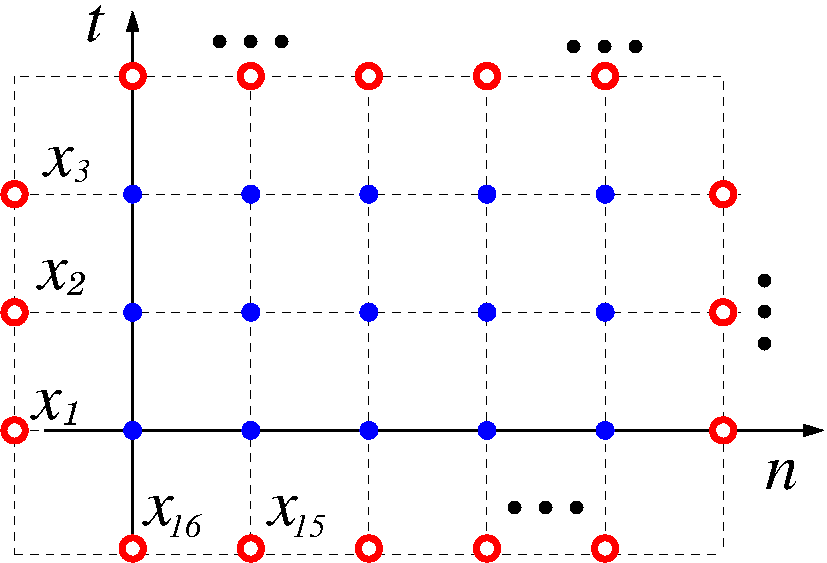
\includegraphics[width=0.33\textwidth]{rectangular_domain}
\hspace{2mm}
(b)\;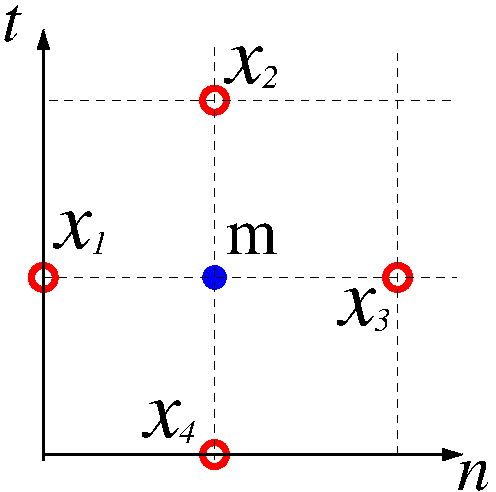
\includegraphics[width=0.23\textwidth]{symbol_block_one}
  \hspace{2mm}
(c)\;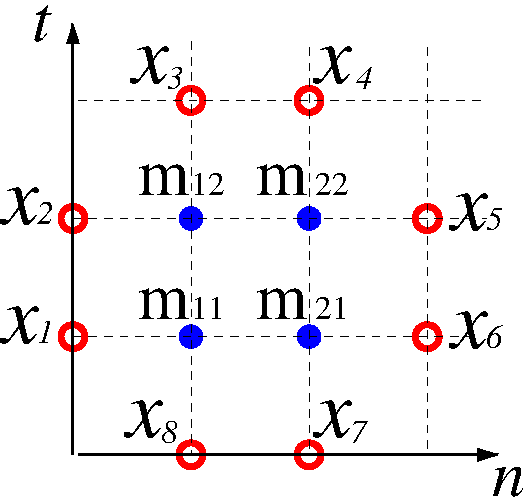
\includegraphics[width=0.23\textwidth]{symbol_block}
	\caption{\label{fig:block2x2}
(Color online)
(a) A $[5\!\times\!3]$ domain $\R$ on the
2\dmn\ lattice. The red (open) circles indicate the boundary
$\partial \R$. For each  point $x_i\in \partial\R $, there exists a unique
adjacent point within the domain $\R$.
{\Brick s} $\MmR$ for
(b) $\R = [1\!\times\!1]$,  and
(c) $\R = [2\!\times\!2]$  domains, together with the corresponding
boundary points
$\partial\R=\{\ssp_{1}, \ssp_{2},  \ssp_{3}, \ssp_{4}\}$  and
$\partial\R=\{\ssp_{1}, \ssp_{2},  \cdots, \ssp_{8}\}$, respectively.
   }
\end{figure}


\subsubsection{Example: $\R = [2\!\times\!2]$ measure.}
\label{exam:block2x2}

For the {\brick}
\beq
\Mm=
        \left[\begin{array}{c}
\Ssym{12} \Ssym{22}   \\
\Ssym{11} \Ssym{21}
              \end{array}\right]
\ee{eq:block2x2}
the 8\dmn\ polytope $\Pol_{\Mm}$ is  parametrized by the boundary
$\partial \R$   points, \reffig{fig:block2x2}\,(c).  They  satisfy $0
\leq \ssp_{i} <1,  i=1,\dots 8$, supplemented by the four inequalities:
\beq
 0< P_k(x_1,\dots,x_8) \leq \edit{8\,s(s^2-1)}, \qquad k=1,2,3,4,
\ee{eq:block2x2Inequalities}
where
\begin{eqnarray*}
\fl P_1=
\edit{2(2s^2-1)}(\ssp_1 +\ssp_{8}+\Ssym{11})
 +\edit{2s}(\ssp_3+\ssp_2+\ssp_6+\ssp_7+\Ssym{12}+\Ssym{21})+2(\ssp_4+\ssp_5+\Ssym{22})\nonumber\\
\fl P_2=\edit{2(2s^2-1)}(\ssp_2 +\ssp_3+\Ssym{12})
 +\edit{2s}(\ssp_1+\ssp_{8}+\ssp_4+\ssp_5+\Ssym{11}+\Ssym{22})+2(\ssp_7+\ssp_6 +\Ssym{21})\nonumber\\
\fl P_3=\edit{2(2s^2-1)}(\ssp_7 +\ssp_6+ \Ssym{21})
 +\edit{2s}(\ssp_1+\ssp_{8}+\ssp_4+\ssp_5 +\Ssym{22}+\Ssym{11})+2(\ssp_2+\ssp_3+\Ssym{12})\nonumber\\
\fl P_4=\edit{2(2s^2-1)}(\ssp_4 +\ssp_5 +\Ssym{22})
 +\edit{2s}(\ssp_3+\ssp_2+\ssp_6+\ssp_7 + \Ssym{12}+\Ssym{21})+2(\ssp_1+\ssp_{8} +\Ssym{11})
\,.
\end{eqnarray*}

These inequalities lead to analytical expressions for $\Pol_{\Mm}$
volumes. A general $\Pol_{\Mm}$ volume is a four-dimensional integral,
whose calculation is lengthy and unilluminating, so we skip it here.
Instead, we evaluate $|\Pol_{\Mm}|$ for cases where some of the
inequalities (\ref{eq:block2x2Inequalities}) are satisfied  for all
points of the hypercube  $\Pol_0=\{x_1, \dots,x_8 \in [0,1)\}$. If all
letters of $\Mm$ belong to the interior alphabet, then all inequalities
hold, and $|\Pol_{\Mm}|=1$. Another easy case is the one where  three out
of four inequalities hold for all points in $\Pol_0$. For example,
consider
\[
       \Mm= \left[\begin{array}{cc}
        \edit{s}-2    & \edit{s}-2 \\
        \underline{2} & \edit{s}-1
              \end{array}\right]
\]
for an even $\edit{s>2}$. Then only the first inequality,
$0<P_1(x_1,\dots,x_8)$, is a non-trivial one, while the rest are
satisfied for all points in $\Pol_0$. Since the center of the hypercube
$\{x_i=1/2, i=1,\dots,8\}$ belongs to  the hyperplane
$P_1(x_1,\dots,x_8)=0$, the polytope $\Pol_{\Mm}$ has the same volume as
half of  the hypercube $\Pol_0$, \ie,  $|\Pol_{\Mm}|=1/2$.

It is also possible to find all {\inadmissible} symbol {\brick s}, with
$|\Pol_{\Mm}|=0$. For {\inadmissible} symbol {\brick s}, one of the
inequalities (\ref{eq:block2x2Inequalities}) must be violated for all
points of the hypercube $\Pol_0$. In particular, any combination of
symbols for $[2\!\times\!2]$ {\brick} that satisfies condition
\[
(2+\Ssym{11})\edit{(2s^2-1)}+(4+\Ssym{12}+\Ssym{21})\edit{s}+ (2+\Ssym{22})\leq 0
\]
is forbidden, \ie, $|\Pol_{\Mm}|=0$. This implies that symbol {\brick s}
  \[
  \left[\begin{array}{cc}
        \underline{2} & \underline{2}  \\
        \underline{2} &  \underline{2}
              \end{array}\right],  \qquad
        \left[\begin{array}{cc}
        \Ssym{12} & \Ssym{22}  \\
        \underline{3} &  \Ssym{21}
              \end{array}\right]
\]
are  {\inadmissible} if either $\Ssym{12}+\Ssym{21}\leq\edit{2s}-6$ and
arbitrary  $\Ssym{22}$, or
$\Ssym{12}+\Ssym{21}=\edit{2s}-5,\Ssym{22}\leq\edit{s}-3$.
Other forbidden $[2\times2]$ {\brick}s  are obtained by
application of the symmetry operations.

\subsubsection{Numerics.}
\label{sect:2Dnumerics}

\begin{figure}	
\begin{center}
(a)\;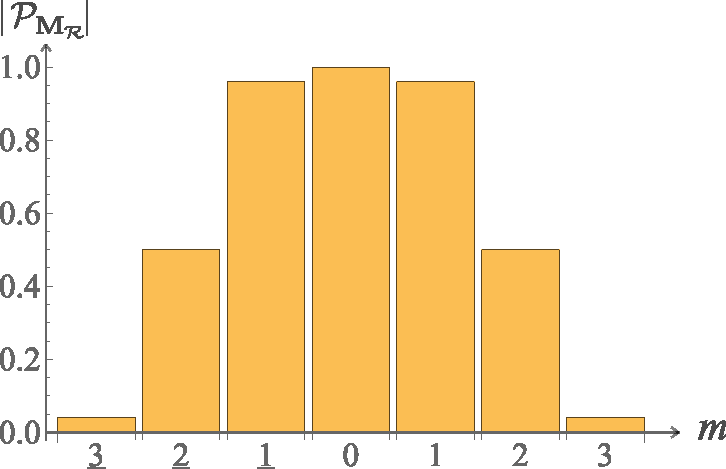
\includegraphics[width=0.35\textwidth]{RJsymbol-a}
  \hspace{4mm}
(b)\;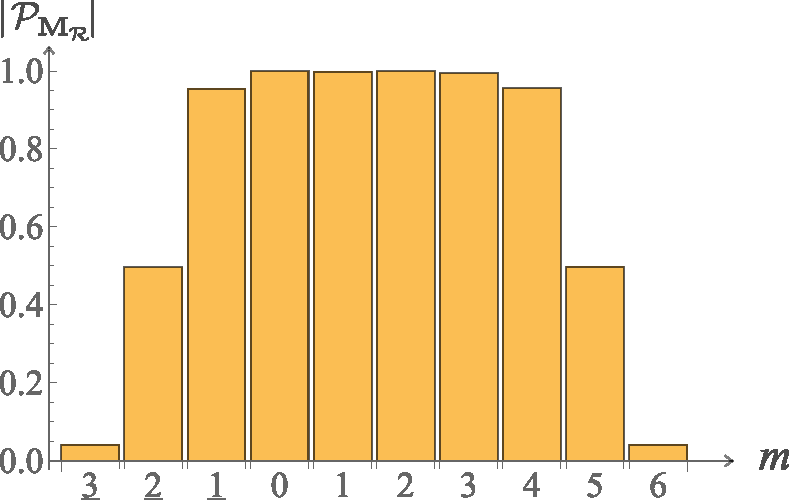
\includegraphics[width=0.35\textwidth]{RJsymbol-b}\\
  \vspace{4mm}
(c)\;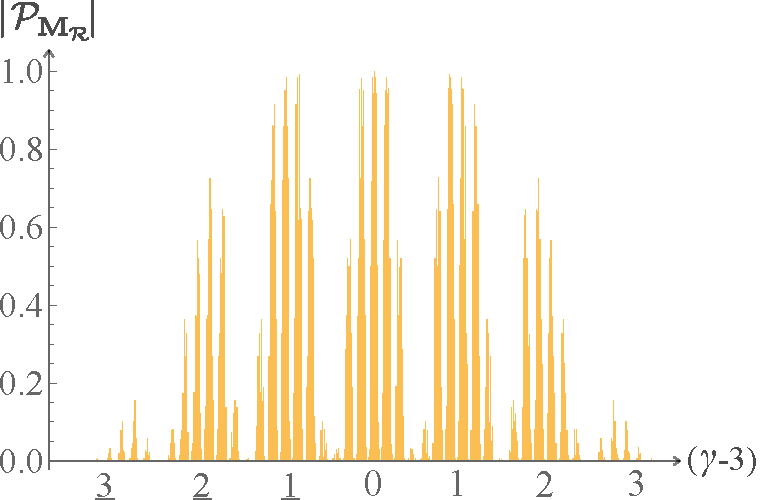
\includegraphics[width=0.36\textwidth]{RJsymbol-c}
  \hspace{4mm}
(d)\;\includegraphics[width=0.36\textwidth]{RJsymbol-d}
\end{center}
\caption{\label{fig:RJsymbol}
Relative frequencies $|\Pol_{\Mm_\R}| = f({\Mm_\R})/{d_\R}$ of {\brick s}
$\MmR$ obtained from long-time numerical simulations ($\sim10^7$
iterations, rounded off to two significant  digits) are in agreement with
the exact formulas of \refeq{exactBlock1x1}.
    (a) $\R=[1\!\times\!1]$ domain, \reffig{fig:block2x2}\,(b), $\edit{s=2}$.
The interior alphabet \refeq{2dCatLattAlph} consists of only one letter
$\Ai=\{0\}$, with the corresponding polytope of maximal volume,
$|\Pol(0)|=1$.
    (b) $\R=[1\!\times\!1]$, $\edit{s=7/2}$.
The maximum frequencies are attained for the four letters
\refeq{2dCatLattAlph7} from the interior alphabet $\Ai=\{0,1,2,3\}$.
The {\brick s} $\MmR$
over the $\R=[2\!\times\!2]$ {\spt} domain, \reffig{fig:block2x2}\,(c),
can be represented as numbers  \refeq{block2x2bases=3}
in base $\edit{2s}+3$.
    (c) For $\R=[2\!\times\!2]$,  $\edit{s}=2$,
the only combination of interior symbols that attains the maximum measure
is $\Ssym{11}=\Ssym{12}= \Ssym{21}=\Ssym{22}=0$.
    (d) For $\R=[2\!\times\!2]$, $\edit{s=7/2}$,
the interior alphabet \Ai\ \refeq{2dCatLattAlph7} has $4$ letters, so
there are $4^4$ \brick s that attain the maximum measure.
    }
\end{figure}

The  volumes  of $\Pol_{\Mm}$ evaluated analytically are found to be
consistent with the measure  of a given {\brick} \Mm\ obtained by
numerical simulations of trajectories with random initial conditions.

While in the $\R=[1\!\times\!1]$ case it was possible to plot the single
symbol {\brick} $\Mm$ measures $\Msr(\Ssym{j})$ along a single, integer
$j$ labelled axis, as in \reffig{fig:RJsymbol}\,(a) and (b), the $\R =
[2\!\times\!2]$ has four sites
\(
z\in\{11,12,21,22\}
\,.
\)
A way to map the array \refeq{eq:block2x2} onto a line is to write it as
\beq
\gamma(\MmR) = \gamma_1.\gamma_2 \gamma_3 \gamma_4
\ee{block2x2bases=3}
in base $\edit{2s}+3$, where
$\gamma_k\in\{0,1,\cdots,\edit{2s}+2\}$ are the symbols $\Ssym{ij}$
shifted into nonnegative integers,
\[
(\gamma_1,\gamma_2,\gamma_3,\gamma_4)
= (\Ssym{11}+3,\Ssym{12}+3,\Ssym{21}+3,\Ssym{22}+3)
\,.
\]
Estimates of the corresponding measures $\Msr(\MmR)$  from long-time
numerical Hamiltonian simulations, on a spatially periodic domain of
extent $L=20$, are displayed in this way in \reffig{fig:RJsymbol}\,(c)
and (d), and are in full agreement with the available analytical data. In
particular, whenever all symbols $\Ssym{ij}$ belong to the interior
alphabet, the numerics is consistent with relative frequency
$|\Pol_{\MmR}|=1$.

\section{Families of {\twots}}
\label{sect:twots}

%%%%%%%%%%%%%%%%%%%%%%%%%%%%%%%%%%%%%%%%%%%%%%%%%%%%%%%%%%%%%%%%%%%%%%%
\begin{figure}
\begin{center}
(a) 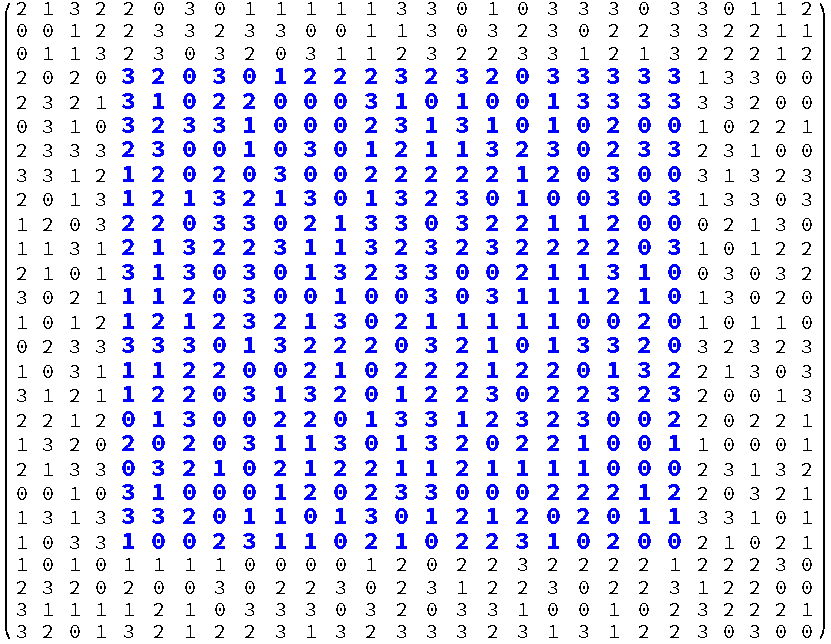
\includegraphics[width=0.45\textwidth]
{AKSs7BlockBorderM1} %\hspace{0.7cm} %color: {AKSs7colrBorderM1}
(b) 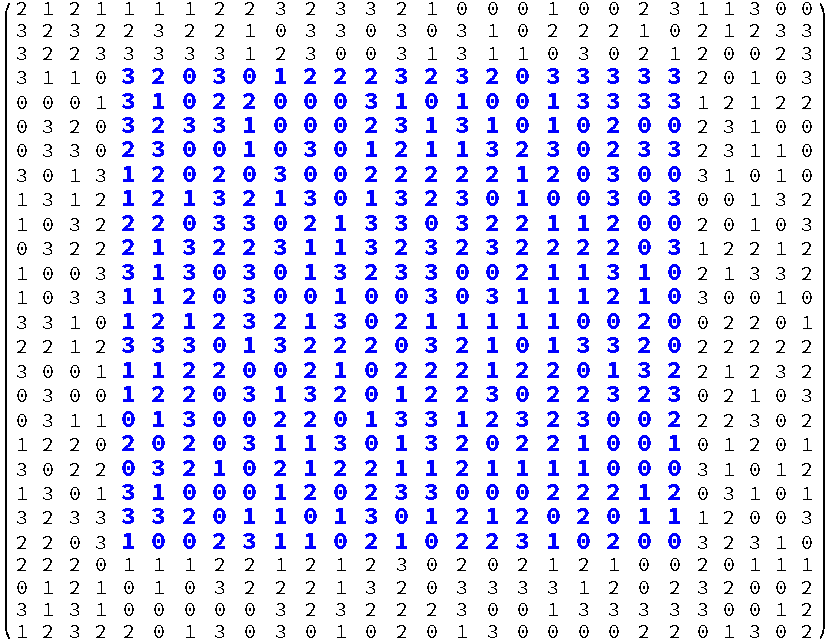
\includegraphics[width=0.45\textwidth]
{AKSs7BlockBorderM2}                 %color: {AKSs7colrBorderM2}
\end{center}
\caption[]{
(Color online)
{\Brick s} $\Mm$, $\Mm'$ encoding  two $[L\!\times\!T] = [28 \times 27]$
{\twots} $\Xx$, $\Xx'$ that shadow each other within the $[19\times 20]$
domain $\R\subset \ZLT$ (bold/blue).
The symbols  over the $\R$ are  drawn randomly from the $\edit{s=7/2}$ interior
alphabet $\Ai=\{0,1,2,3\}$ and are the same for both symbolic {\brick s}
$\Mm$, $\Mm'$. The symbols outside $\R$, also drawn randomly from \Ai,
differ for $\Mm$, $\Mm'$.
}
\label{fig:BGcloseActSymb}  %in blog, color: {fig:AKScloseActSymb}
\end{figure}
%%%%%%%%%%%%%%%%%%%%%%%%%%%%%%%%%%%%%%%%%%%%%%%%%%%%%%%%%%%%%%%%%%%%%%%

%%%%%%%%%%%%%%%%%%%%%%%%%%%%%%%%%%%%%%%%%%%%%%%%%%%%%%%%%%%%%%%%%%%%%%%
\begin{figure} % PC 2019-08-27 replaces \reffig{fig:AKScloseActSp}
\begin{center}
(a) 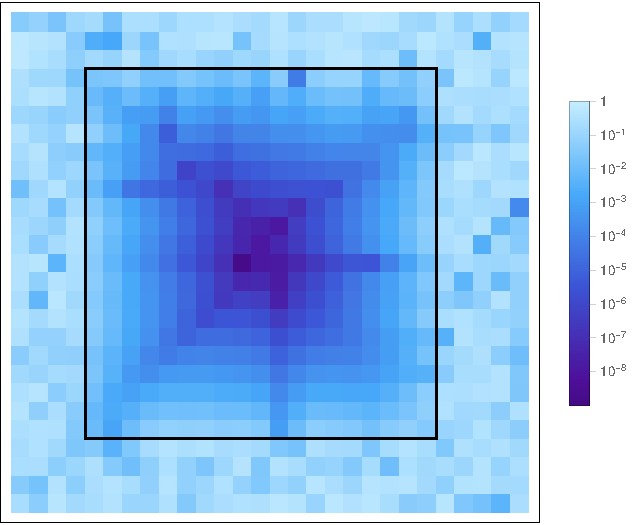
\includegraphics[width=0.45\textwidth]
{AKSLPS12} % elsewhere {AKSs7distM1M2} %\hspace{0.7cm}
(b) 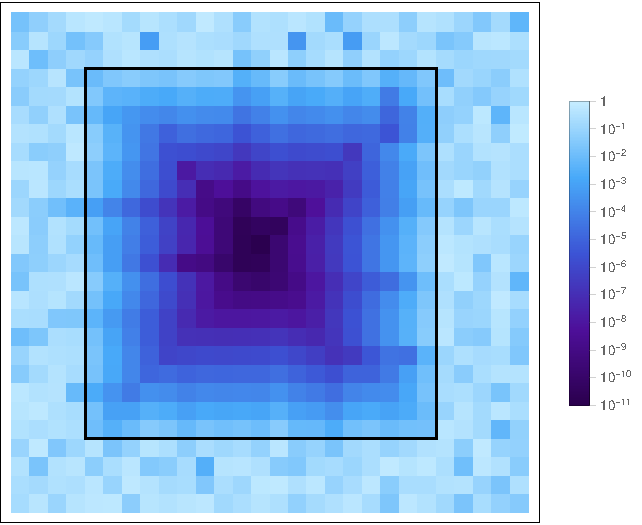
\includegraphics[width=0.45\textwidth]
{AKSLPS12_1} % elsewhere {AKSs7distM1M2log}
\end{center}
\caption[]{\label{fig:AKSLPS12}
(Color online)
The plots of the logarithm of the site-wise distance
\(|x_{z}-x'_{z}|\) of the states $\Xx$, $\Xx'$ of
\reffig{fig:BGcloseActSymb} for
(a)
$\edit{s=7/2}$  and
(b) $\edit{s=13/2}$
illustrate the exponential fall-off of the site-wise distances as one
approaches the center of the shared symbol domain ${\R}$.  The
exponential fall-off towards the center of ${\R}$ is faster for $s=13$.
Outside of the shared domain \R\ the distances are of the order $1$.
}
\end{figure}
%%%%%%%%%%%%%%%%%%%%%%%%%%%%%%%%%%%%%%%%%%%%%%%%%%%%%%%%%%%%%%%%

Linear encoding makes it an easy task to obtain \catlatt\
\refeq{CoupledCats} solutions. Of particular interest are the doubly
periodic solutions (the \spt\ analogs of $d\!=\!1$ cat map \po s), the
\twots\ with periods $L$ and $T$,
\[
          \ssp_{nt} = \ssp_{n+L,t+T},
\qquad    n=1,\cdots ,L,\;\; t=1,\cdots,T
\,,
\]
invariant under  spatial $\Spshift^L$  and temporal $\Tshift^T$ shifts.

Since the interior alphabet \Ai\ corresponds to a full shift
dynamical system,  any $[L\!\times\!T]$ {\brick} of interior symbols
$\Mm= \{\Ssym{z}\in\Ai|z\in \ZLT \}$
over the rectangular \spt\ domain
\[
\ZLT=\{z=(n,t)| n=1,\cdots,L,\;\; t=1,\cdots,T\}
\,,
\] is {\admissible} and generates an \twot\ solution of \refeq{CoupledCats}.
The corresponding {\spt} state  $\Xx =\{\ssp_z, z\in \ZLT\}$ (restricted to the domain $\ZLT$)
is obtained
by taking the inverse of \refeq{CoupledCats}:
\begin{equation}
   \ssp_z=\sum_{z'\in \ZLT} \gp_{zz'} \Ssym{z'}, \qquad    \Ssym{z'}\in \Ai
\,,
\end{equation}
where $\gp_{zz'}$ is the Green's function with periodic boundary
conditions, see \rf{CL18}.
We next use the obtained solutions
to test shadowing  properties of \twots.

\subsection{Partial shadowing}
\label{sect:partShade}

As the first application, we show  in \reffig{fig:BGcloseActSymb} two
$[L\!\times\!T]$ \brick s $\Mm$, $\Mm'$ composed of interior symbols
$m_z\in \Ai$, which coincide within a   rectangular  domain
$\R\subset\ZLT$. In  \reffig{fig:AKSLPS12}, we  show the distances between
the corresponding {\spt} states $\Xx$, $\Xx'$. In agreement with the
results of \refsect{sect:CCMmeasBrick}, the distances between
$\ssp_z\in\Xx$ and $\ssp_z'\in\Xx'$ shrink exponentially as $z$
approaches the center of the domain \R. In other words, \Xx\ and $\Xx'$
shadow each other within the domain \R.

%%%%%%%%%%%%%%%%%%%%%%%%%%%%%%%%%%%%%%%%%%%%%%%%%%%%%%%%%%%%%%%%%%%%%%%
\begin{figure}
\begin{center}
 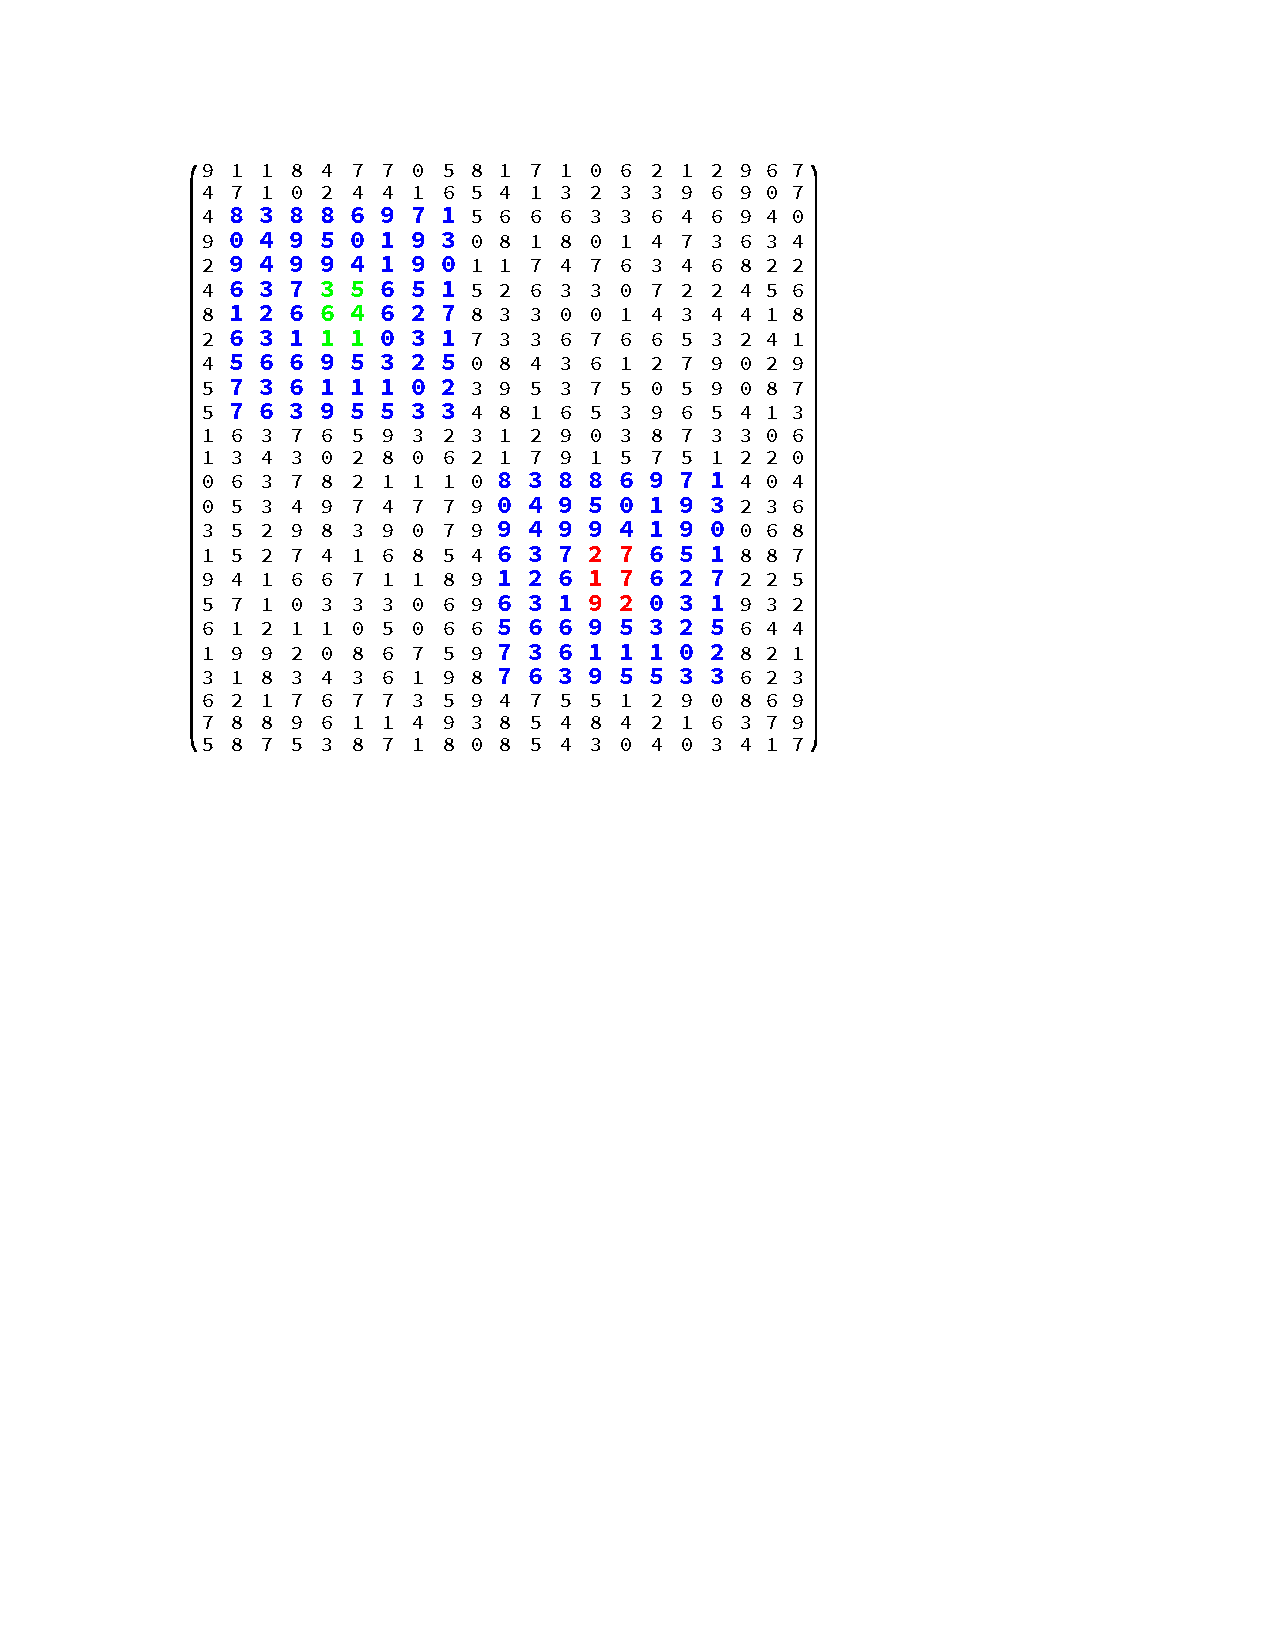
\includegraphics[width=0.48\textwidth]{AKSs13TwoBlocksM1}
 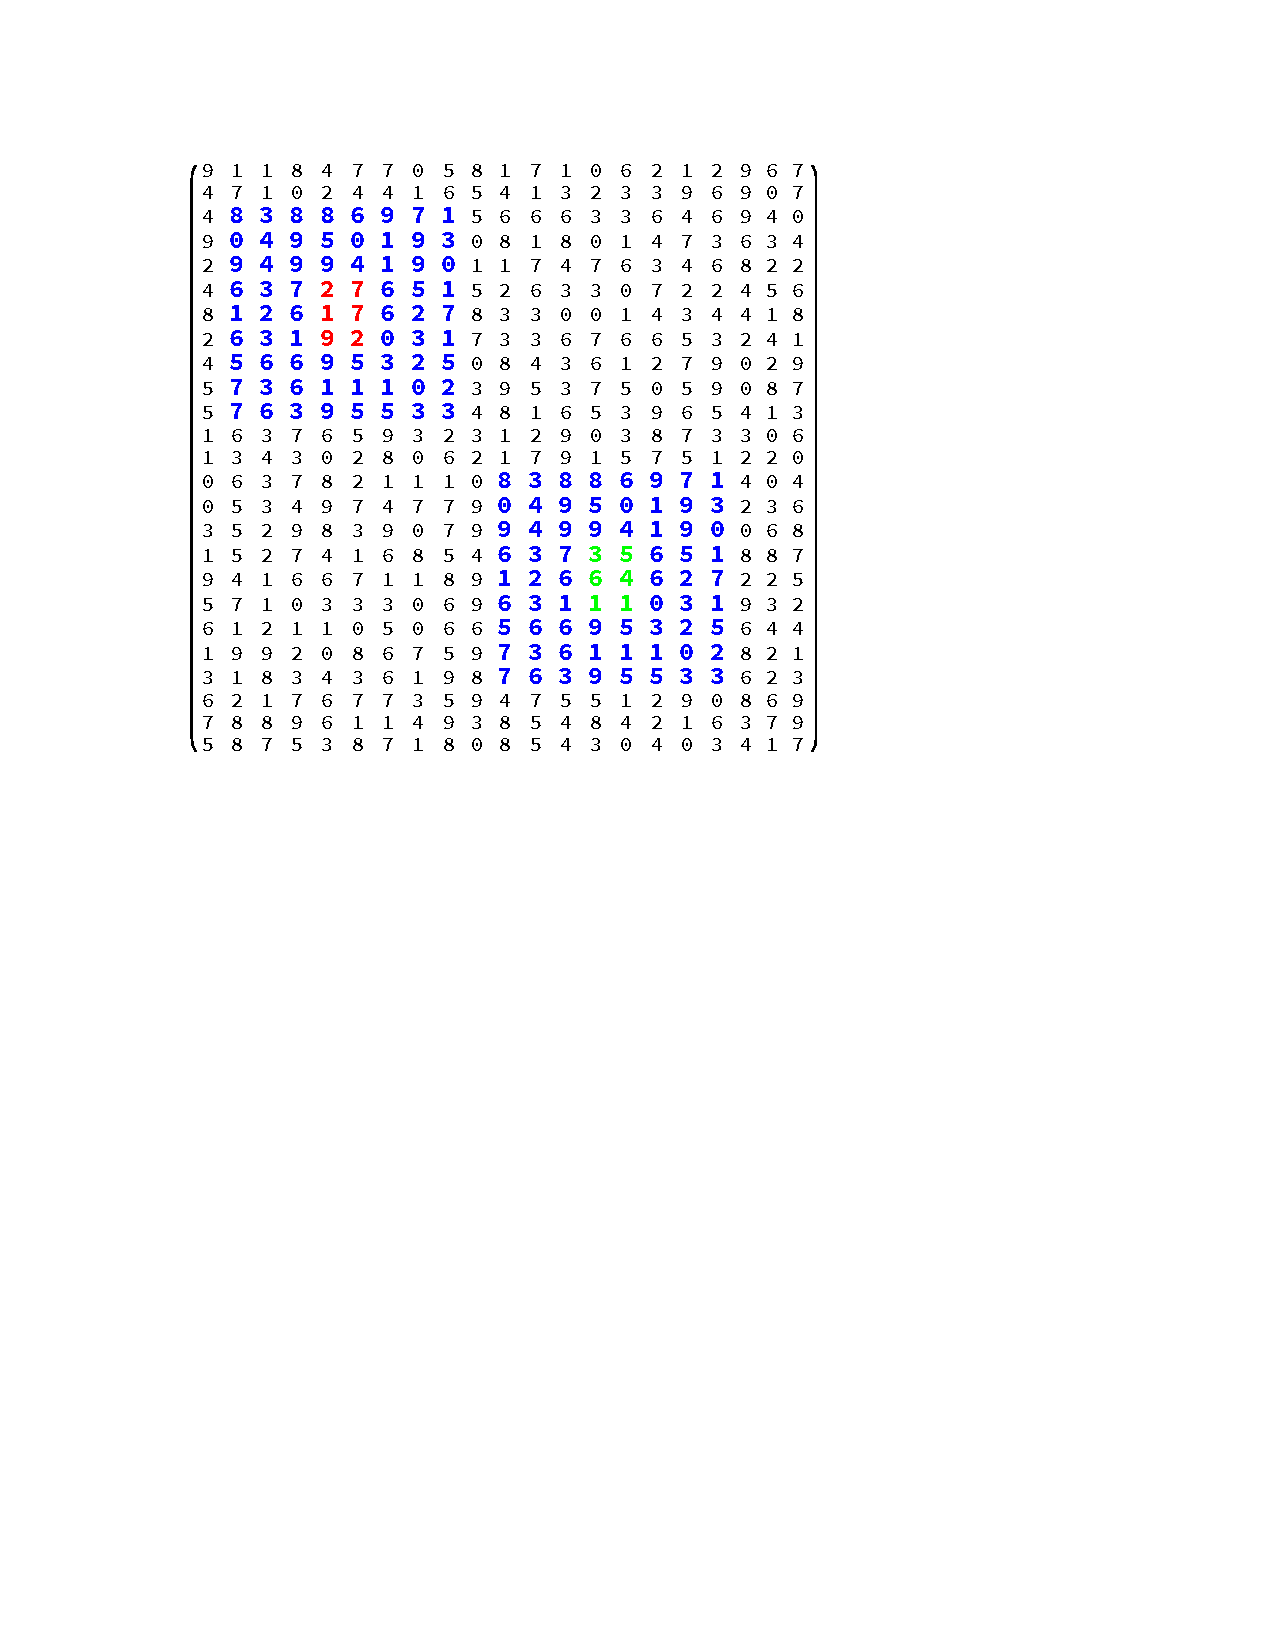
\includegraphics[width=0.48\textwidth]{AKSs13TwoBlocksM2}
\end{center}
\caption[]{\label{fig:AKSs13TwoBlock}
(Color online)
Symbol \brick s $\Mm_1$, $\Mm_2$ of two $[25\times25]$ \twots\ $\Xx_1$,
$\Xx_2$, with
annular
(encounter) domains $\R_1$ and $\R_2$ indicated
in blue (bold).
The symbols are drawn randomly from the interior alphabet $\Ai$ for
$\edit{s=13/2}$. The two \brick s $\Mm_1$, $\Mm_2$ are related by the permutation
of symbol \brick s over  the interior domains $A_1$, $A_2$ (red and green,
respectively). Any $[3\times3]$ symbol {\brick} $\Mm^{[3\times 3]}$
appears the same number of times in both $\Mm_1$ and $\Mm_2$, and the two
\twots\ $\Xx_1$ and $\Xx_2$ shadow each other at every point.
    }
\end{figure}
%%%%%%%%%%%%%%%%%%%%%%%%%%%%%%%%%%%%%%%%%%%%%%%%%%%%%%%%%%%%%%%%%%%%%%%

%%%%%%%%%%%%%%%%%%%%%%%%%%%%%%%%%%%%%%%%%%%%%%%%%%%%%%%%%%%%%%%%%%%%%%%
\begin{figure}
\begin{center}
   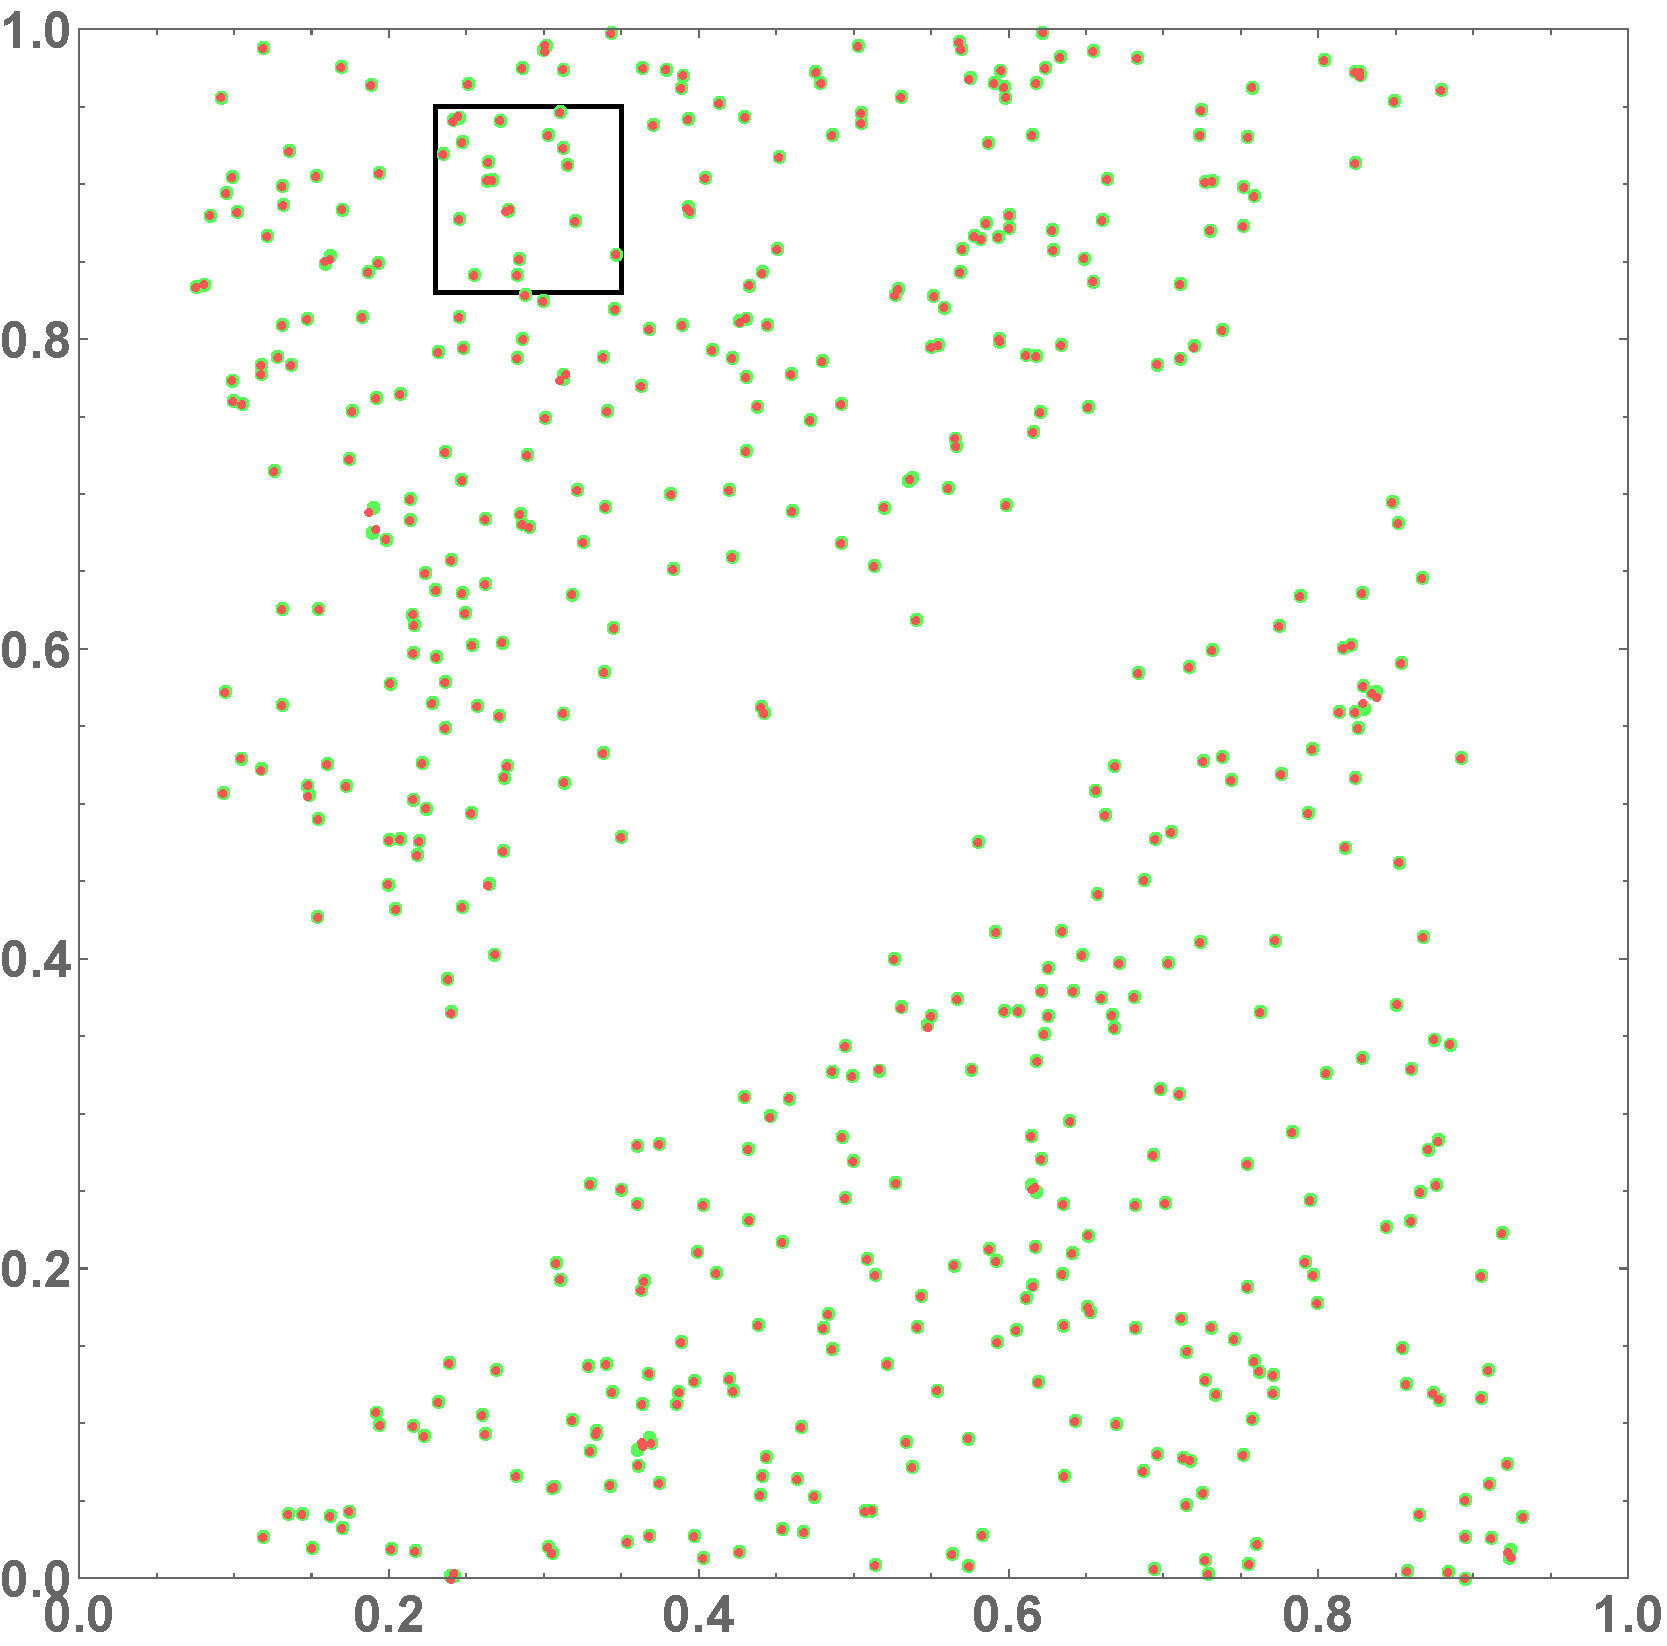
\includegraphics[width=0.48\textwidth]
{AKSs13TwoBlocksG1}
   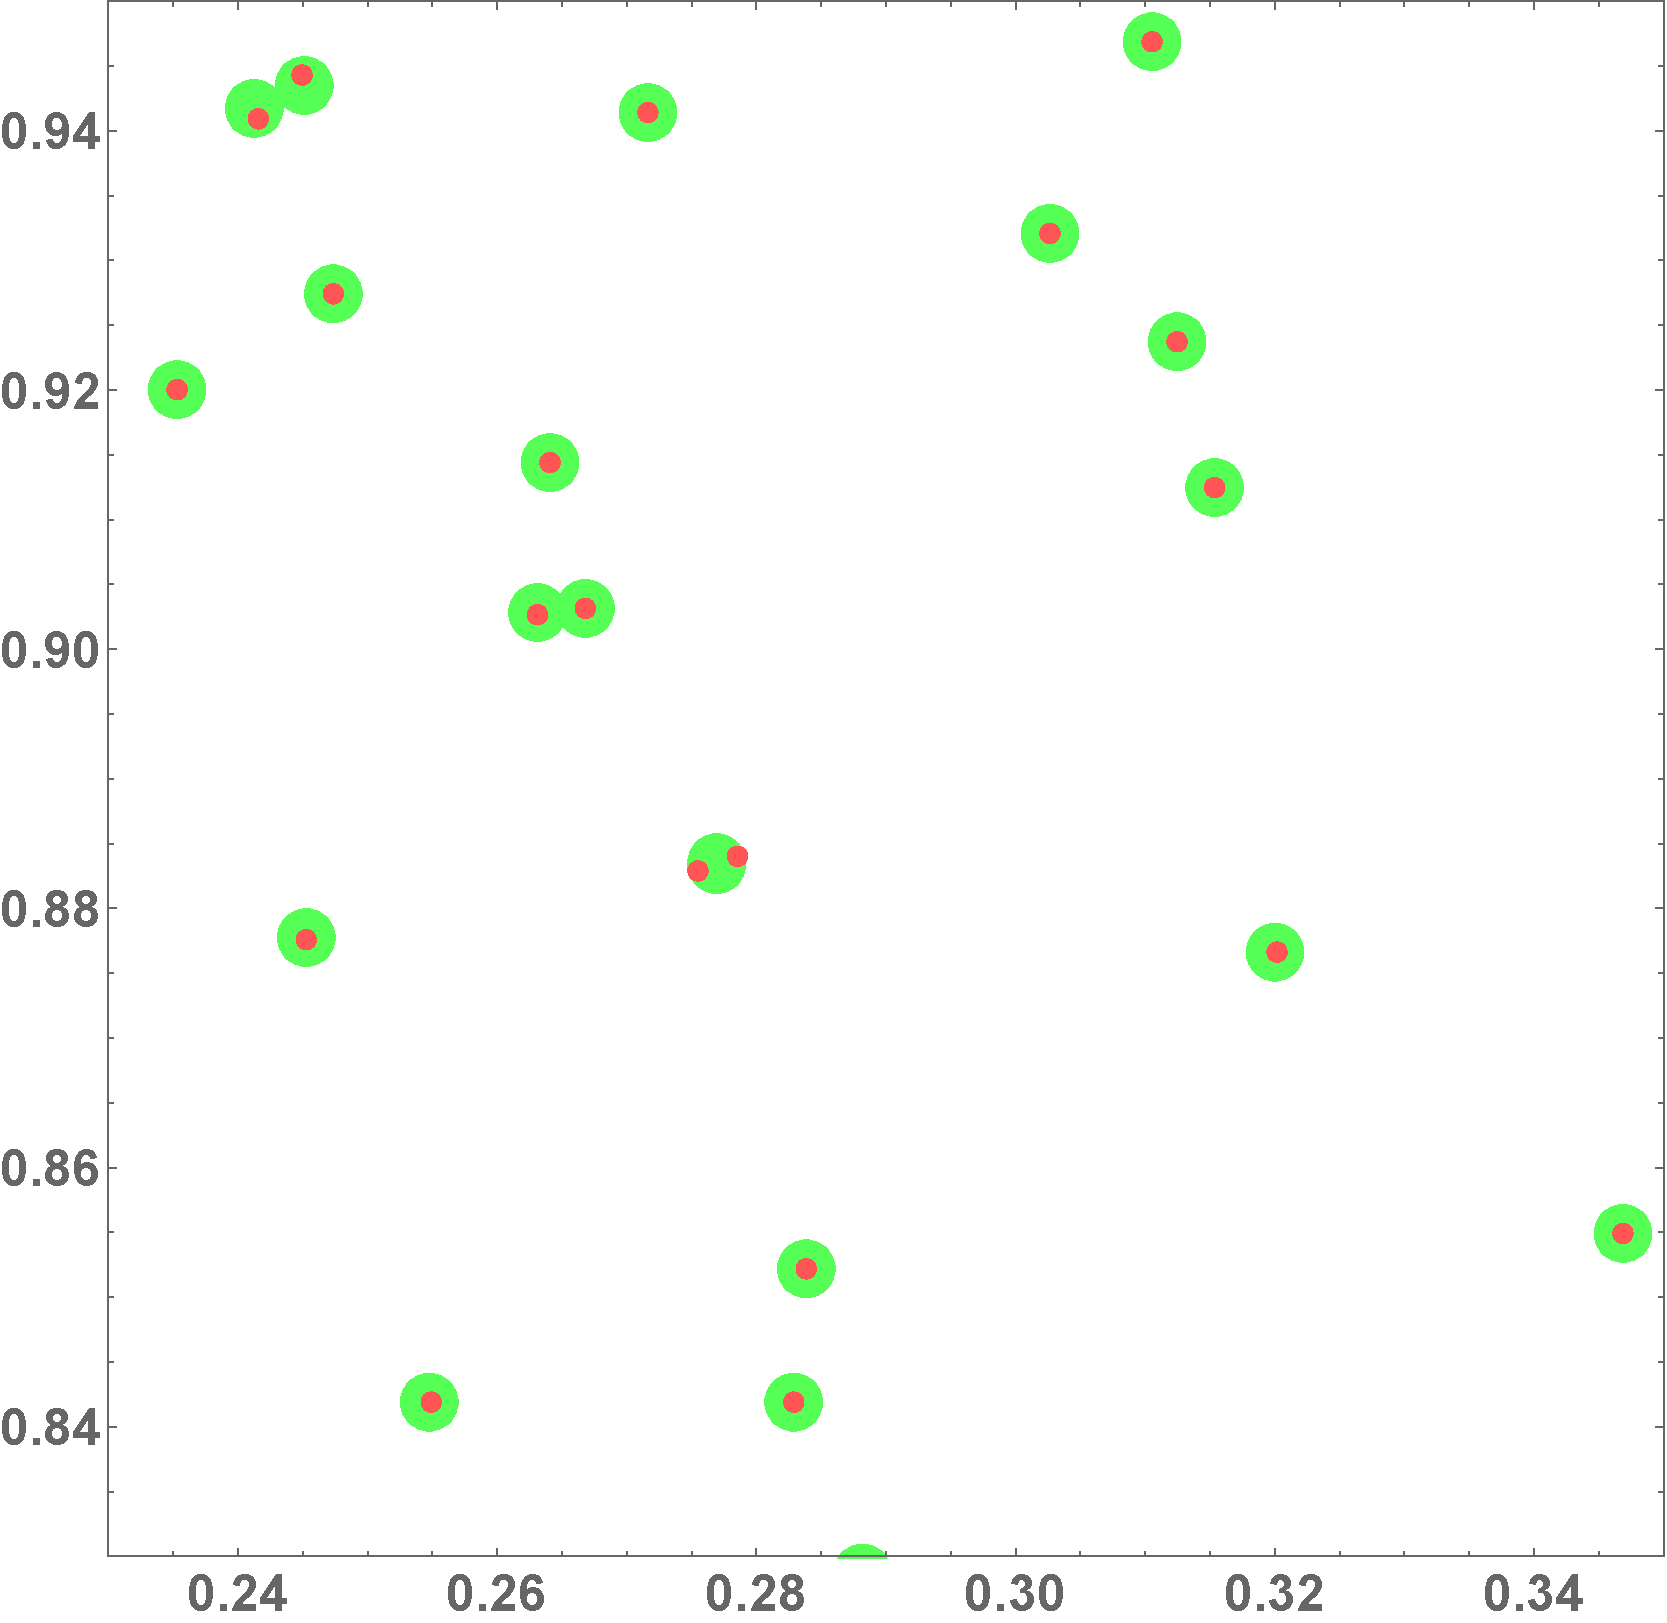
\includegraphics[width=0.48\textwidth]
{AKSs13TwoBlocksG2}
\end{center}
\caption[]{\label{fig:AKSs13TwoBlocks}
(Color online)
(left)
Hamiltonian coordinate-\-momentum representation of the two \twots\
$\Xx_1, \Xx_2$ of \reffig{fig:AKSs13TwoBlock}. This Hamiltonian
representation is explained in \refappe{sect:HamiltonCatLatt}.
(right)
An enlargement of the square in (left).  The small (red)  circles indicate
points  $(q^{(1)}_z, p^{(1)}_z)$  of   $\Xx_1$. The large  (green)
circles correspond to the  points $(q^{(2)}_z, p^{(2)}_z)$  of   $\Xx_2$.
The solutions pair nearly perfectly, except for the points
from the encounter domains $z\in \R_1\cup \R_2$,  where some small
deviations can be  observed.
    }
\end{figure}
%%%%%%%%%%%%%%%%%%%%%%%%%%%%%%%%%%%%%%%%%%%%%%%%%%%%%%%%%%%%%%%%%%%%%%%


\subsection{Full shadowing}
\label{sect:fullShade}

%%%%%%%%%%%%%%%%%%%%%%%%%%%%%%%%%%%%%%%%%%%%%%%%%%%%%%%%%%%%%%%%%%%%%%%
\begin{figure}
    \begin{center}
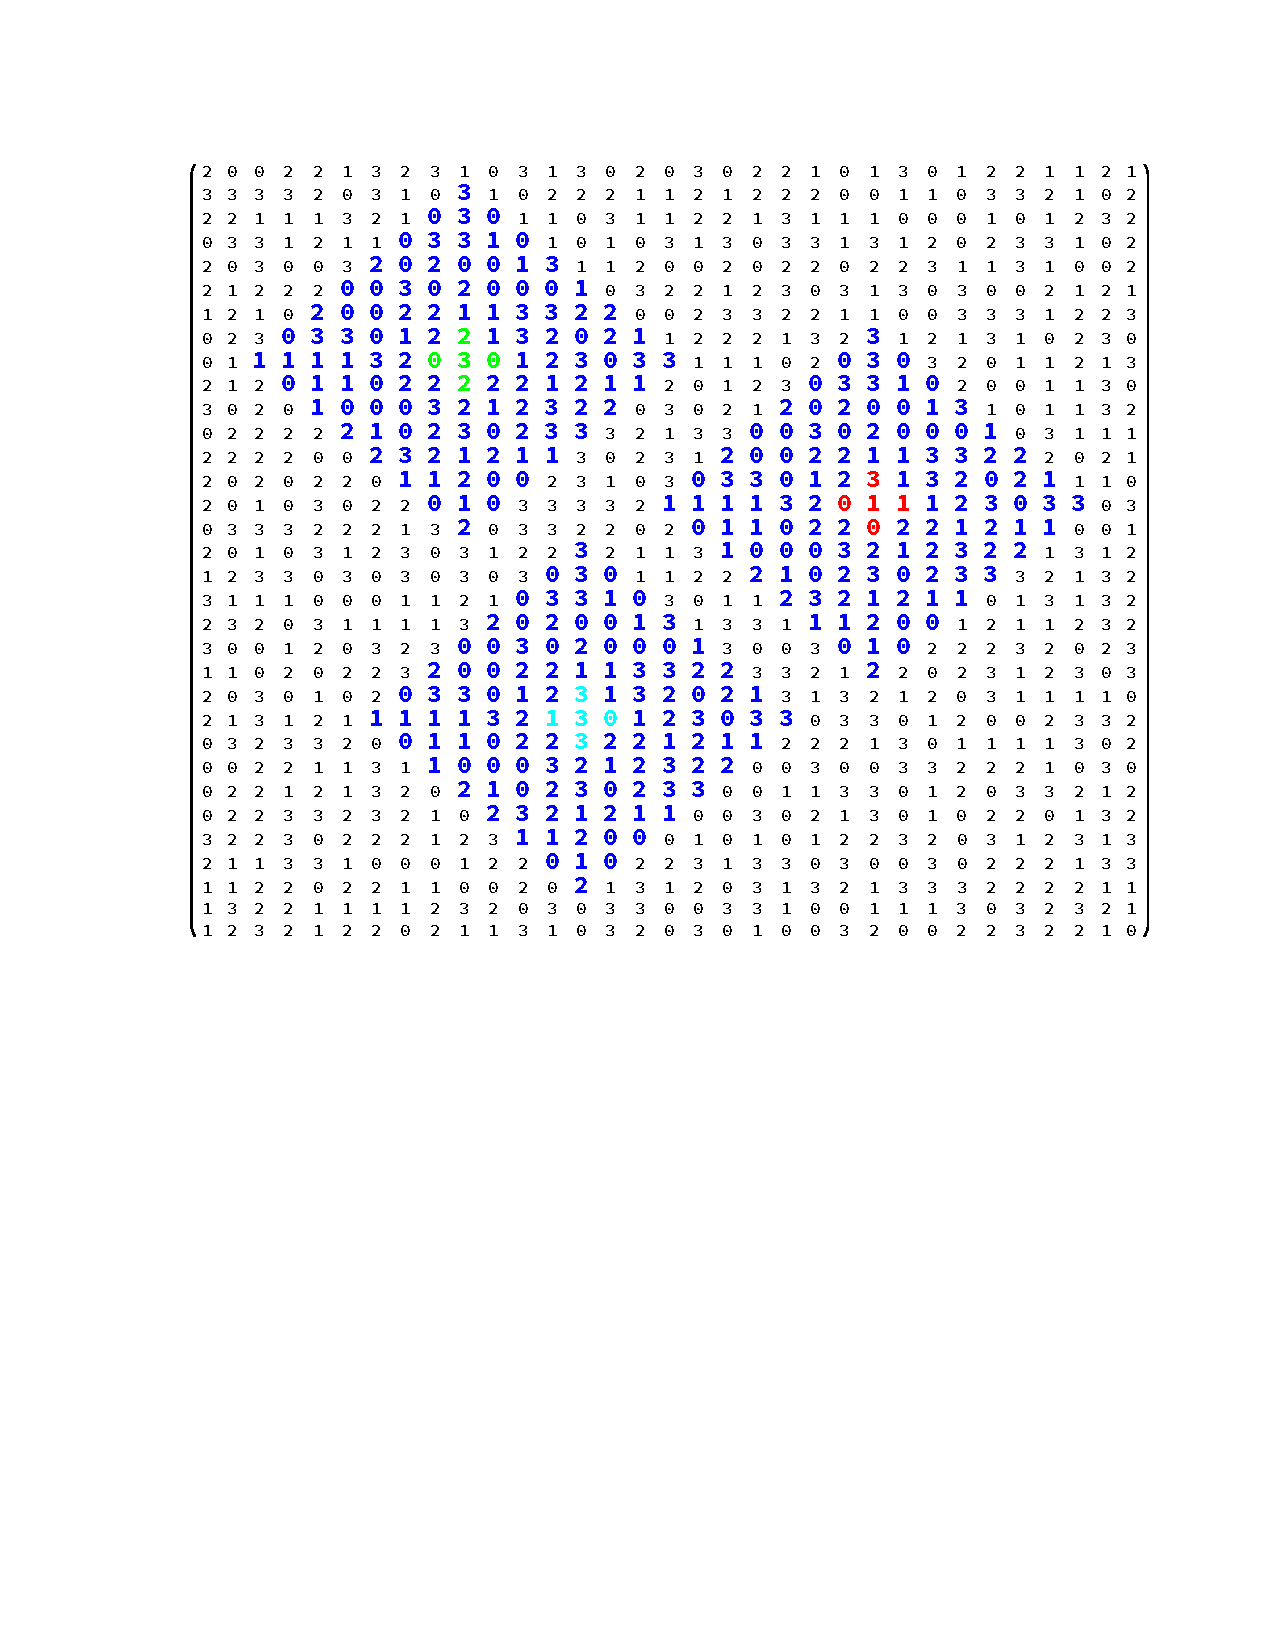
\includegraphics[width=0.48\textwidth]{AKSs7ThreeDiamondsM1}
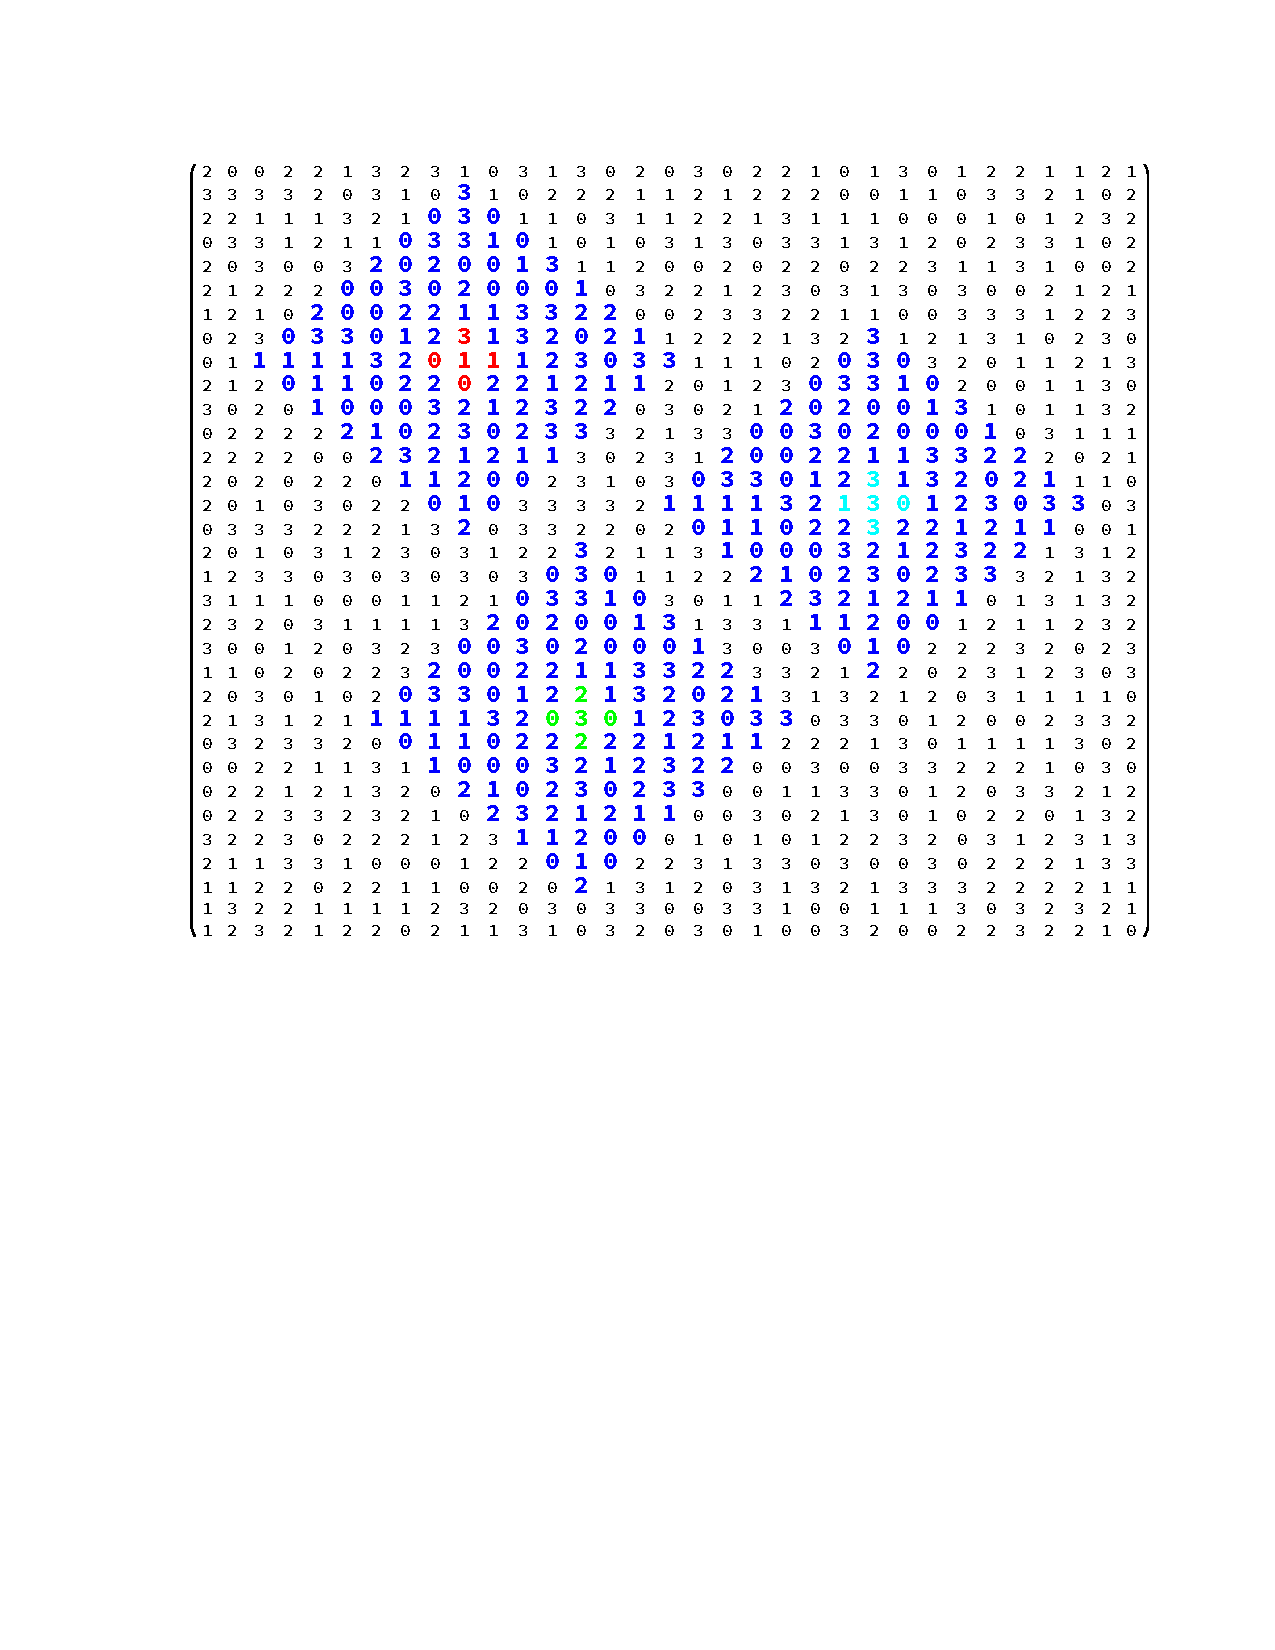
\includegraphics[width=0.48\textwidth]{AKSs7ThreeDiamondsM2}~\hspace{0.3cm}%
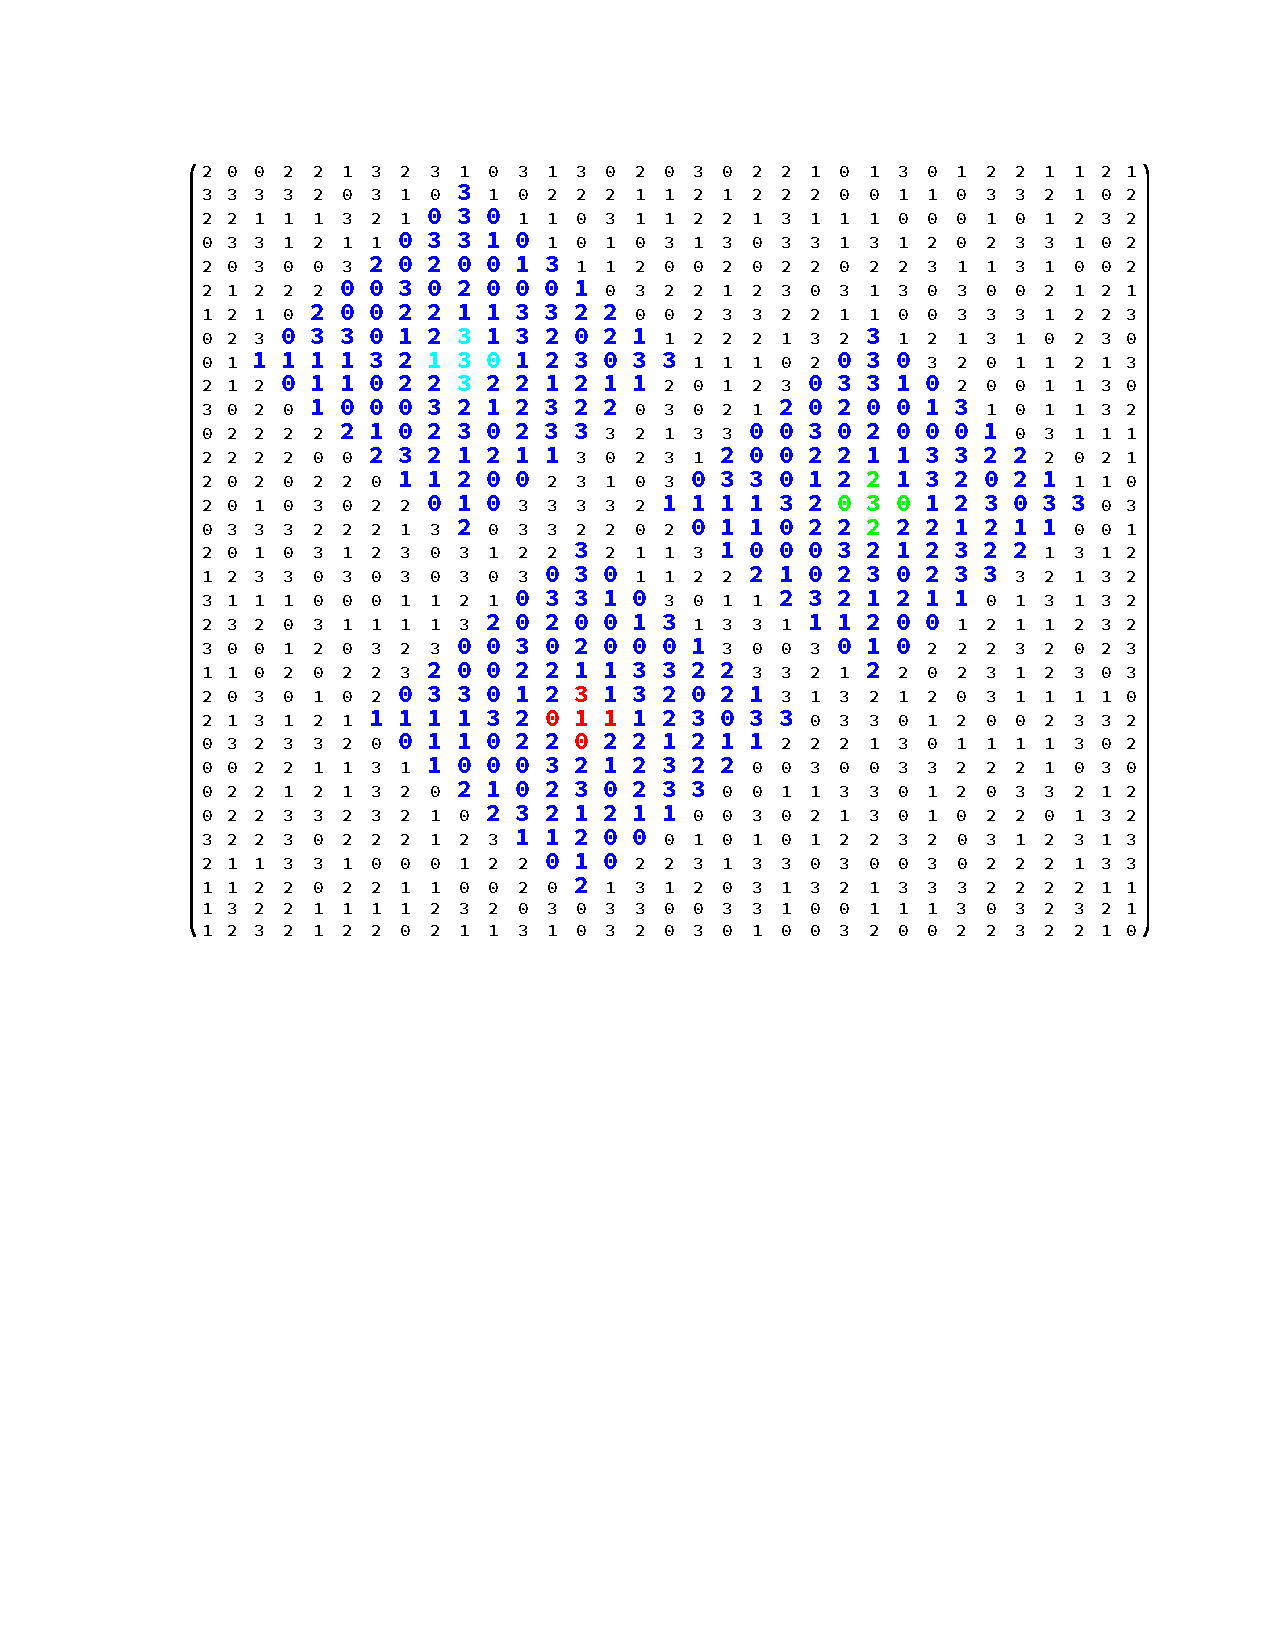
\includegraphics[width=0.48\textwidth]{AKSs7ThreeDiamondsM3}
    \end{center}
\caption[]{
(Color online)
Symbol \brick s $\Mm_1, \Mm_2, \Mm_3$ of three $[33\times33]$ \twots\
$\Xx_1, \Xx_2, \Xx_3$, with the 3-encounter diamond-shaped
domains $\R_1, \R_2, \R_3$  indicated in blue (bold). The symbols are
drawn randomly from the interior alphabet $\Ai$ for $\edit{s=7/2}$.
$\Mm_1\to\Mm_2\to\Mm_3$ are related by the cyclic permutation of the
symbol \brick s  within  the interior domains (red, green, light  blue).
Any distinct $[4\!\times\!4]$ symbol {\brick} $\Mm^{[4\times 4]}$ appears
the same number of times in each \twot\ (or not at all).
        }
\label{fig:AKSs13TwoBlock2}
\end{figure}
%%%%%%%%%%%%%%%%%%%%%%%%%%%%%%%%%%%%%%%%%%%%%%%%%%%%%%%%%%%%%%%%%%%%%%%

%%%%%%%%%%%%%%%%%%%%%%%%%%%%%%%%%%%%%%%%%%%%%%%%%%%%%%%%%%%%%%%%%%%%%%%
\begin{figure}
\begin{center}
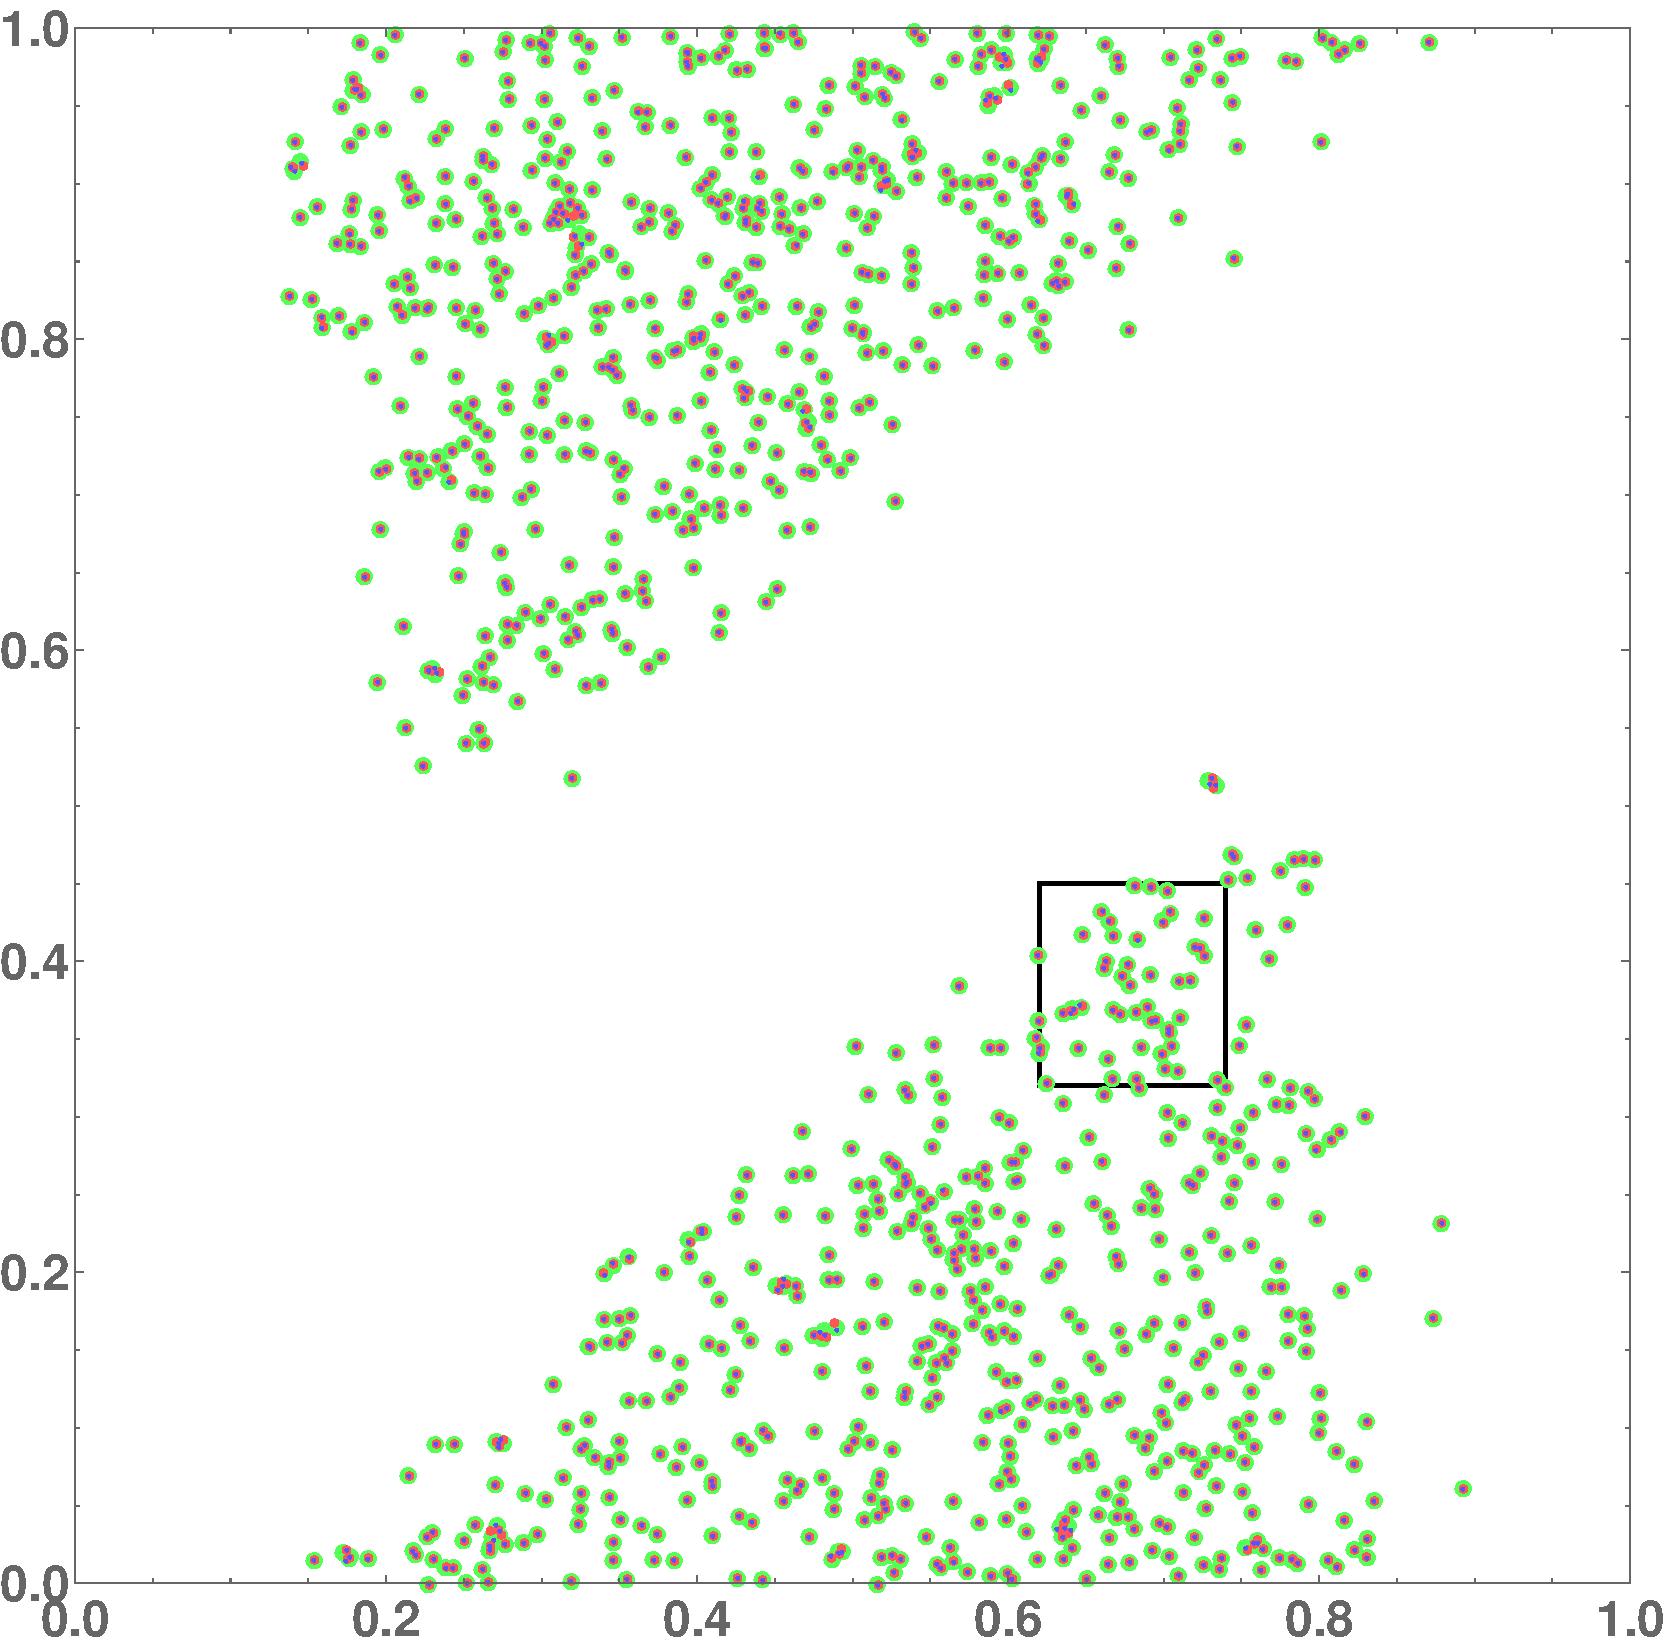
\includegraphics[height=0.48\textwidth]
{AKSs7ThreeDiamondsG1}
   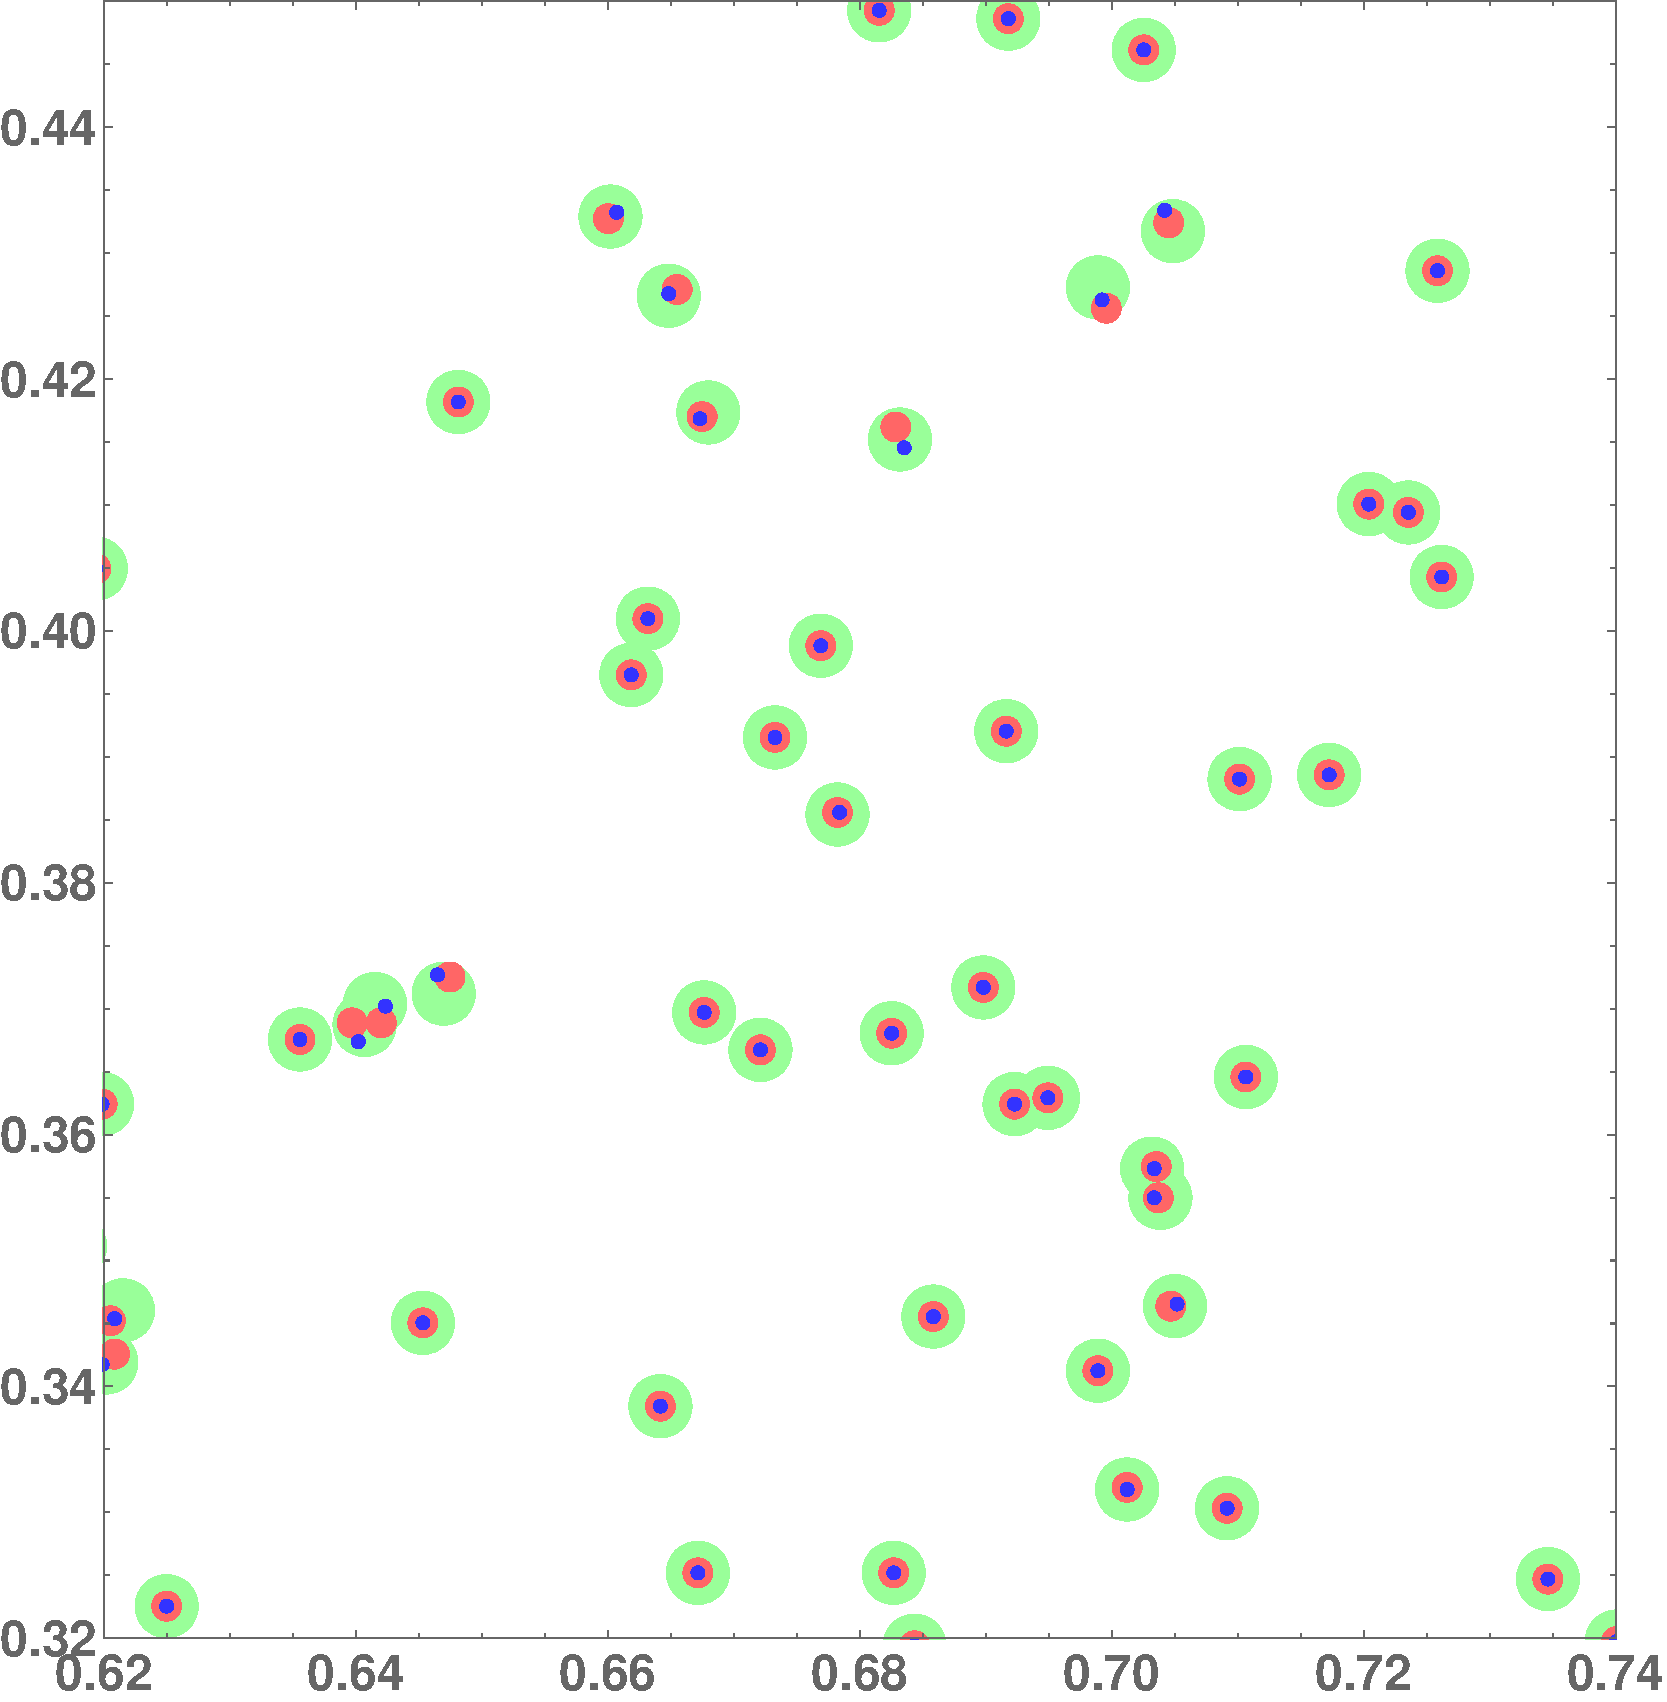
\includegraphics[height=0.48\textwidth]
{AKSs7ThreeDiamondsG2}
\end{center}
\caption[]{\label{fig:AKSs13TwoBlocks1}
(Color online)
(left) Hamiltonian coordinate-\-momentum representation $(q^{(i)}_z,p^{(i)}_z)$,
$i=1,2,3$
of the three \twots\  $\Xx_i$,
$i=1,2,3$  of \reffig{fig:AKSs13TwoBlock2},
shown as centers of the green, red and blue circles. (right)
An enlargement of the (left) \statesp.  Note that the three \twots\ $\Xx_i$
form almost perfect triplets except for the points
from the encounter domains, $z\in \R_1\cup\R_2\cup\R_3$  where some
deviations can be  observed.
        }
\end{figure}
%%%%%%%%%%%%%%%%%%%%%%%%%%%%%%%%%%%%%%%%%%%%%%%%%%%%%%%%%%%%%%%%%%%%%%%

The \twots\ $\Xx$ and $\Xx'$ of the above example shadow each other only
partially - outside of the subdomain $\R$ their points are not paired. On the
other hand, it turns out to be possible to find different \twots\
solutions of \refeq{CoupledCats} which shadow each other at every point
of $\ZLT$. Such solutions, referred as partners,  play an important role
in the semiclassical treatment of the corresponding quantum \edit{problem}, since
their action differences are small, see
\refrefs{SieRic01,MuHeBrHaAl04,GutOsi13a,GutOsi13,GutOsi15}. We briefly
recall here the construction of partner solutions in  $d=2$ setting,
following \refref{GutOsi15}.

Let $\{\R_1, \dots, \R_{m}\},\; \R_j\subset \R$, be ${m}$ non-overlapping
domains obtained  by spacetime shifts $(n,t)\to(n+n_i,t+t_i,)$,
$i=2,\dots {m}$ of a given domain $\R_1$,
\[
\R_i=\Spshift^{n_i}\Tshift^{t_i}\,\R_1
\,,\qquad
\R_i\cap\R_j=\emptyset \mbox{ for } i\neq j
\,.
\]
Examples of such domains (referred to as ``${m}$-encounters'')
are given in \reffigs{fig:AKSs13TwoBlock}{fig:AKSs13TwoBlock2}. Assume
that the domain $\R_1$  has  an annular shape  with a non-empty interior
$A_1$, and an exterior $C_1=\ZLT \setminus{A}_1\cup\R_1$. We define the
width  $\ell$ of ``annulus'' $\R_1$   by determining the largest
$[\ell\!\times\!\ell]$ square domain $\R^{[\ell\times\ell]}$ that can fit
into $\R_1$ i.e., $\R^{[\ell\times\ell]}$ that has no simultaneous
intersections with both the hole and the exterior. In other words, $\ell$
is the maximum integer such that either
$A_1\cap\R^{[\ell\times \ell]}=\emptyset$, or
$C_1\cap\R^{[\ell\times \ell]}=\emptyset$,
for any translation of $\R^{[\ell\times \ell]}$. All encounter domains
$\R_i$ have the same width $\ell$, as they are translations of each
other.

Now,  let \brick\
\(
\Mm\equiv\Mm_1=\{\Ssym{z}\in\Ai|z\in\R\}
\)
be a  $[L\!\times\!T]$ symbolic representation of a \catlatt\
\refeq{CoupledCats} \twot\ state $\Xx\equiv\Xx_1$, such that it contains the same
{\brick} of symbols over each of the   subdomains
$\R_1,\dots,\R_{m}$,
\[
\Mm_{\R_1}=\Mm_{\R_2}= \dots = \Mm_{\R_{m}}
\,,
\]
where $\Mm_{\R_i}$ stands for the restriction of $\Mm$ to the domain
$\R_i$. Provided that the $m$  interior domains $A_1,\dots A_m$ have
different symbolic content, $\Mm_{A_i}\neq\Mm_{A_j}$ for $i\neq{j}$, we
can generate $m!$ distinct {\brick s} $\Mm_a, a=1,\dots m!$ by permuting
symbol \brick s $\Mm_{A_i}$ over the \edit{domains} $A_1,\dots A_m$. This leads to
${m}!$ distinct \twots\
$\Xx_1, \dots \Xx_{{m}!}$
whose symbol {\brick s} $\Mm_{1}, \dots \Mm_{{m}!}$ share the following
property: each distinct $[\ell\!\times\!\ell]$ square symbol {\brick}
appears one and the same number of times in all $\Mm_{a}, \, a=1,\dots,
m!$, with  $\ell$ being  the width of the encounter domains $\R_i$. In
other words, if a   $[\ell\!\times\!\ell]$ symbol {\brick}
$\Mm^{[\ell\times\ell]}$
appears in $\Mm_1$ a number of times (or zero times),  it must appear the
same number of times in  the encoding $\Mm_{a}$ of any other \twot\
$\Xx_a, a\neq1$.

By the shadowing property, this in turn implies that all $\Xx_1, \dots
\Xx_{{m}!}$  pass through approximately the same points of the \statesp\
but in a different {\spt} `order'. The degree of their closeness is
controlled by the parameter $\ell$. The larger $\ell$ is, the closer two
different $\Xx_a$,  $\Xx_b$ come  to each other in the \statesp. In
\reffigs{fig:AKSs13TwoBlocks}{fig:AKSs13TwoBlocks1} we illustrate these
pairings for families of \twot\ solutions which symbolic representations
are shown in \reffigs{fig:AKSs13TwoBlock}{fig:AKSs13TwoBlock2},
respectively.

\section{Summary and discussion}
\label{sect:summary}

In this paper, we have analyzed the {\catlatt} \refeq{LinearConn}
linear encoding. We now summarize our main findings.

The finite alphabet of symbols \A\ encoding system's dynamics has been shown
to split into interior \Ai\ and exterior \Ae\ parts, where only symbolic
\brick s containing external symbols require non-trivial grammar
rules. \Brick s  composed of only interior symbols are {\admissible}
and   attain one and the same measure for a given \edit{domain \R}.
Furthermore, the measure of a general {\brick} factorizes into product of a
constant factor $d_\R$ and the geometric one  $|\Pol_\R|$ which  can be
interpreted as a volume of certain type of polytope  in the Euclidean space
whose dimension is determined by the length of the boundary of \R. While
$d_\R$ is fixed by  \R, $|\Pol_\R|$ depends on the symbolic content and attains
maximum value $1$ for \brick s  of interior symbols. In addition, it has been
shown that a  local  {\brick}  of symbols determines approximate positions of
the corresponding \statesp\ points within an error
decreasing exponentially with  the size of the {\brick}.

The  number  of letters, $\edit{2s-3}$, of the interior alphabet  \Ai\ grows
linearly with the increasing stretching parameter $s$, while the exterior
alphabet \Ae\ always consists of the 6 letters. In
the limit of large $s$,  the \brick s of a finite size affected by the
exterior letter pruning rules can be neglected,  as their total measure
tends to zero.   This implies that as $s$ grows, the dynamics of the
{\catlatt} map approaches a Bernoulli process. In particular, by
\refeq{SpatiotemporalEntropy} the ratio between the metric   entropy
$h_\Msr$ of the {\catlatt} and the topological entropy $\log (\edit{2s-3})$  of
the full $(\edit{2s\!-\!3})$-shift   converges  to $1$, as
$\edit{s}\to\infty$.

As an application of these results we have constructed several examples
of partner \twots\ composed of interior symbols which visit the same
regions in the \statesp, but in different {\spt} ``orders''. Such
\twots\ shadowing each other are expected to play an important role in
the semiclassical treatment of the corresponding quantum models.

\subsection{Discussion and future directions}

Remarkably, as far as the linear encoding is concerned, the above results
hold both for the {cat map} and its coupled lattice generalization. In
both cases, the  proofs rely only upon ellipticity of the operator $\Box$
and the linearity of the equations. It is very plausible  that the same
results hold for the lattices $\integers^d$  of an arbitrary dimension $d$.
\edit{
Indeed, the companion paper\rf{CL18} makes claim that its
\po\ theory formulation applies to \catlatt\ in any dimension.
    }%end \edit
Furthermore, the restriction to
the integer valued matrices in the definitions of maps appears unnecessary. Cat
map is a smooth version of the sawtooth map, defined by the
same equation \refeq{OneCat}, but for a real (not necessarily integer) value
of $s$. The linear encoding for the {saw map} has been analyzed in
\refref{PerViv} and its extension  to a coupled $\integers^d$ model along the
lines of the present paper seems to be straightforward. Also,  in the current
paper we stuck to  the Laplacian  form of $\Box$.   Again this seems to be
too restrictive and extension to other elliptic  operators of higher order
should be possible. Such operators necessarily appear within the models
with higher range of interactions.

A physically necessary extension of  current setting would be addition of an
external periodic potential ${V}$ to \refeq{LinearConn}, rendering this a
nonlinear problem,
 \begin{equation}
 (\Box -\edit{d(s-2)}+ {V}'(\ssp_z)) \ssp_z = \Ssym{z}, \qquad z\in \integers^{d}
 \,. \label{LinearConnPerturbed}
\end{equation}
As long as the perturbation ${V}$ is sufficiently weak, this lattice map can
be conjugated to the linear {\catlatt}, with ${V}=0$.
This approach has been used in \refref{GutOsi15} to construct partner
{\twots} for perturbed cat map lattices.
On the other hand, for a sufficiently strong perturbation, such a conjugation
to linear system is no longer possible. Also, let us note that the lattice
models like  \refeq{LinearConnPerturbed} can be seen  as discretized versions
of PDEs arising from the Hamiltonian field theories.
In this respect, it would be of  interest  to study whether our results  can
be extended to the continuous, PDE setting.


Finally, there are many intriguing open questions about the quantum
properties of {\catlatt}s. Starting with the work of Hannay and
Berry\rf{HanBer80}, quantum cat maps have provided deep insights into
``single particle'' quantum chaos, see e.g. \refref{Keating91, Dana02,
Creagh94, ValSar99, KurRud00}. In the same spirit, quantization of the
{\catlatt} could serve as an inspiring model  for ``many-body'' quantum
chaos\rf{GutOsi15, AWGBG16, AWGBG17, AGBWG18}. One of its  most striking
features is the  dynamical self-duality, with spatial and temporal
evolutions being completely equivalent. Due to their remarkable features,
quantum lattice models with   such properties are currently attracting
much interest. Such self-dual models  exhibit properties of
``maximally-chaotic''  quantum systems\rf{BeKoPr18, AWGG16, BWAGG19}, and
yet turn out to be exactly solvable at the thermodynamical limit, with
correlations between local operators\rf{BeKoPr19-4}, the local-operator
entanglement\rf{BeKoPr19-9, GBAWG20, ClaLam20}, and  the time evolution of
the entanglement entropies\rf{BeKoPr19-1, GopLam19} exactly calculable.
It would be interesting to investigate whether similar results can be
established for the {\catlatt} map.


%%%%%%%%%%%%%%%%%%%%%%%%%%%%%%%%%%%%%%%%%%%%%%%%%%%%%%%%%%%%%%%%%%%%%%%%%%
\ack
Work of B.~G. and P.~C. was supported by the family of late G. Robinson,
Jr..  B.~G. acknowledges  support from  the Israel Science
Foundation through grant No.~2089/19.

%To obtain a simple heading of `Appendix' use the code
%\verb"\section*{Appendix}". If it contains numbered equations, figures or
%tables the command \verb"\setcounter{section}{1}" must follow it.
%%%%%%%%%%%%%%%%%%%%%%%%%%%%%%%%%%%%%%%%%%%%%%%%%%%%%%%%%%%%%%%%%%%%%%%%%%
\appendix

\section{Lattice Green's functions}
\label{sect:Green}

\subsection{Green's  function for 1\dmn\ lattice}

Consider the {cat map} equation \refeq{OneCat} with a delta function
source term
\begin{equation}
 (-\Box+s-2) \gd_{ij}=\delta_{ij}, \qquad i,j \in \integers^1
\,.
\label{GreenFun0}
\end{equation}
The corresponding free, infinite lattice Green's function $\gd_{ij}=\gd_{i-j, 0}$
is given by\rf{varcyc,PerViv}
\beq
\gd_{t 0}=\frac{1}{\pi}\int_{0}^{\pi}\frac{\cos(tx)}{s-2\cos x } dx
   = \ExpaEig^{-|t|}/(\ExpaEig-\ExpaEig^{-1})
\,,
\ee{GreenFun00}
with $s=\ExpaEig+\ExpaEig^{-1}$, $\ExpaEig>1$, as may be verified by
substitution.

\medskip

\paragraph{Dirichlet boundary conditions:}
In this case the Green's function $\gd$  satisfies
\refeq{GreenFun0}, but,  in addition, is subject to the  Dirichlet
boundary conditions:
\[ \gd_{0j} = \gd_{i0}= \gd_{\ell +1,j} = \gd_{i,\ell+1}=0
\,.
\]

It is possible to determine $\gd$ in two different ways.
The first one  is to use  the fact that $ \gd_{ij}=(\D^{-1})_{ij}$, where
$ \D$ is tridiagonal $[\ell\!\times\!\ell]$ matrix
\[\D= \left(\begin{array}{ccccccc}
s & -1 & 0 & 0 &\dots &0&0 \\
-1 & s & -1 & 0 &\dots &0&0 \\
0 & -1 & s & -1  &\dots &0 & 0 \\
\vdots & \vdots &\vdots & \vdots & \ddots &\vdots &\vdots\\
0 & 0 & \dots &  \dots &\dots &-1 & s  \end{array} \right )
\,.
\]
Since $\D$ is of a tridiagonal form,  its inverse can be  found explicitly.

An alternative  way to evaluate   $\gd_{ij}$   is to use \edit{the free
Green's function \refeq{GreenFun00}} and take anti-periodic sum (similar
method can be used for  periodic and Neumann  boundary conditions)
\[   \gd_{ij}=\sum_{n=-\infty}^{\infty} \gd_{i,j+2 n(\ell+1)}- \gd_{i,-j+2 n(\ell+1)}. \]
This approach has an advantage of being  easily extendable  to
$\integers^2$ case. After substituting $\gd$ and taking the sum one
obtains
\begin{equation}
 \gd_{ij}=  \begin{array}{ll}
        \frac{U_{i-1}(s/2)U_{\ell-j}(s/2)}{U_{\ell}(s/2)} \qquad &\mbox{for } i\leq j\\
        \frac{U_{j-1}(s/2)U_{\ell-i}(s/2)}{U_{\ell}(s/2)} \qquad &\mbox{for } i> j .
        \end{array}
\,,
\label{BGtempCatGF}
\end{equation}
where \(
U_n(s/2)=\frac{\sinh (n+1)\Lyap}{\sinh \Lyap}
\,
\)
are Chebyshev polynomials of the second kind, and  $e^\Lyap=\ExpaEig$.
Note that the Green's function is strictly positive for both boundary
conditions.

\subsection{Green's  function for 2\dmn\ square lattice}
\label{sect:Green2D}

The free Green's function
$\gd(z,z')\equiv \gd(z-z',0)\equiv \gd_{z z'}$
solves  the equation
\begin{equation}
 (-\Box+\edit{2s}-4)\gd_{z z'}=\delta_{zz'}
\,,\qquad
  z=(n,t) \in \integers^2
\,.
\label{GreenFun000}
\end{equation}
The solution is given by the double integral\rf{Martin06}
\beq
 \gd_{z0}=\frac{1}{\edit{2}\pi^2}\int_{0}^{\pi}\int_{0}^{\pi}
           \frac{\cos(nx)\cos(ty)}{\edit{s-\cos x -\cos y}} dx dy
 \,,
\ee{GreenFun1}
which, in turn, can be recast into single integral form,
\bea
 \gd_{z0} &=& \frac{1}{2\pi^3}\int_{-\infty}^{+\infty}d\eta\int_{0}^{\pi}\int_{0}^{\pi}
   \frac{\cos(nx)\cos(ty)}{(\edit{s}-2\cos x -i\eta)(\edit{s} -2\cos y+i\eta) } dx dy
    \continue
    &=&
 \frac{1}{2\pi}\int_{-\infty}^{+\infty}d\eta\,
 \frac{\mathcal{L}(\eta)^{-n}\mathcal{L}^*(\eta)^{-t}}{|\mathcal{L}(\eta)-\mathcal{L}(\eta)^{-1}|^2 }
\,,
\label{GreenFun2}
\eea
where
\beq
\mathcal{L}(\eta)+\mathcal{L}(\eta)^{-1}= \edit{s}+i\eta, \qquad  | \mathcal{L}(\eta)|>1
\,. \ee{Lfunc}

The above equation can be thought as the integral over a product of two
$\integers^1$ functions:
\beq
 \gd_{z0} =
 \frac{1}{2\pi}\int_{-\infty}^{+\infty}d\eta\,
                 \gd_{n 0}(\edit{s}+i\eta) \gd_{t 0}(\edit{s}-i\eta)
\,.
\ee{GreenFun3}
An alternative representation is given by modified Bessel
functions $I_n(x)$ of the first kind\rf{Martin06}:
\beq
\gd_{z0} =\int_{0}^{+\infty}d\eta\,e^{-\edit{s\eta/2}} I_n(\eta) I_t (\eta)
\,,
\ee{GreenFun4}
which demonstrates that $ \gd_{z z'}$ is
positive for all $z=(n,t)$.
The representation (\ref{GreenFun4})
enables explicit evaluation of the $n=t$ diagonal elements
in terms of a Legendre function,
\[
 \gd_{z0}=\frac{1}{2\pi i}Q_{n-1/2}(\edit{s^2/2}-1 ),\qquad
        \edit{s^2/2}-1 >1, \quad z=(n,n)
 \,.
\]

\paragraph{Dirichlet boundary conditions.}
Consider next the Green's function $\gd_{zz'}$ which  satisfies
\refeq{GreenFun000} within the rectangular domain
\(
\R=\{ (n,t) \in
\integers^2 |1 \leq n\leq \ell_1 , 1 \leq t\leq \ell_2    \}
\)
and vanishes at its boundary $\partial \R$, see \reffig{fig:block2x2}(a).
By applying the same method as in the case of 1\dmn\ lattices we  get
\begin{eqnarray*}
\gd_{zz'}
&=&\sum_{j_1,j_2=-\infty}^{+\infty}\!\!
\gd_{n-n'+2j_1(\ell_1+1), t-t'+2j_2(\ell_2+1)} +
\gd_{n+n'+2j_1(\ell_1+1),t+t'+2j_2(\ell_2+1)}\\
& &\qquad -\gd_{n-n'+2j_1(\ell_1+1), t+t'+2j_2(\ell_2+1)}
  -\gd_{n+n'+2j_1(\ell_1+1),t-t'+2j_2(\ell_2+1)}
\,,
\end{eqnarray*}
where $\gd_{zz'}$ is the free Green's function \refeq{GreenFun1}.
Substituting  \refeq{GreenFun3} yields
the \spt\ Green's function as a convolution of the two 1\dmn\
Green's functions \refeq{BGtempCatGF}
\begin{equation}
 \gd_{z z'}  =\frac{1}{2\pi}\int_{-\infty}^{+\infty}d\eta\,
              \gd_{nn'}(\edit{s}+i\eta)  \gd_{tt'}(\edit{s}-i\eta)
\,.
\label{DirGreenFun1}
\end{equation}

\paragraph{Exponential decay of Green's function.}
From \refeq{DirGreenFun1} we have a bound on the magnitude of \edit{the}
Green's function,
\bea
    &&|\gd_{z z'}|  \leq \frac{1}{2\pi}\int_{-\infty}^{+\infty}d\eta\,
              |\gd_{nn'}(\edit{s}+i\eta)|\,|\gd_{tt'}(\edit{s}-i\eta)|=
    \continue
    &=&
\int_{-\infty}^{+\infty} \frac{d\eta}{2\pi}\,
 \left( \frac{|\mathcal{L}|^{-|n-n'+1|}|\mathcal{L}|^{-|t-t'+1|} }{|\mathcal{L}-\mathcal{L}^{-1}|^2 }\right)\left(\frac{ \K_{n}K_{\ell_1 -n'+1}\K_{t}\K_{\ell_2 -t'+1} }{ \K_{\ell_1} \K_{\ell_2}}\right)
\,,
\label{GreenFunIneq}
\eea
where  $\mathcal{L}(\eta)$ is the root of the  equation (\ref{Lfunc})
with the largest absolute value, and
\[ %beq
 \K_{j}(\eta) =|1-\mathcal{L}(\eta)^{-2j}|, \qquad j=1,2,\dots \,.
\] %ee{KDef}
We now show that the first factor in the integrand of  (\ref{GreenFunIneq})
decays  exponentially with increasing $n-n'$, $t-t'$, while the second
one is bounded by a constant, and consequently
the Green's function $\gd_{zz'}$ decays exponentially
with increasing \spt\ distance between lattice points $z$ and $z'$.

By  (\ref{Lfunc}) we have
\[
  |\mathcal{L}(\eta)-\mathcal{L}(\eta)^{-1}|^2 =|(\edit{s}+i\eta)^2-4|
  \,.
\]
A lower bound on $|\mathcal{L}(\eta)|$ follows from the observation that
for $\edit{s>2}$  the  minimum of
$|\mathcal{L}(\eta)|$ is achieved at $\eta=0$. Indeed, from  the identity
\[
\left(\frac{\edit{s}}{|\mathcal{L}(\eta)|+|\mathcal{L}(\eta)|^{-1}}\right)^2
+ \left(\frac{\eta}{|\mathcal{L}(\eta)|-|\mathcal{L}(\eta)|^{-1}}\right)^2=1
\]
we obtain
\[
\frac{s/2}{|\mathcal{L}(\eta)|+|\mathcal{L}(\eta)|^{-1}}\leq 1,
\]
which, in turn, implies
\begin{equation}
|\mathcal{L}(\eta)|\geq \mathcal{L}(0)= e^\nu >1, \qquad  \cosh \nu =\edit{s/2}
\,.
\label{LBound}
\end{equation}
The lower and upper bounds  on functions $\K_{j}(\eta)$ follow,
 \beq
 2>1 + |\mathcal{L}(\eta)^{-2j}| \geq \K_{j}(\eta) \geq 1 - |\mathcal{L}(\eta)^{-2j}| > 1- e^{-2\nu}.
\ee{KBound}
Inserting  (\ref{KBound}), (\ref{LBound}) into  (\ref{GreenFunIneq}) yields
 \beq
 |\gd_{zz'}|< C\exp(\nu|n-n'|+\nu|t-t'|)
\,,
\ee{GreenFunIneqFinal}
where
\begin{equation}
C=\left(\frac{2}{\sinh \nu}\right)^2 \int_{-\infty}^{+\infty}
        \frac{d\eta}{2\pi}\,|(\edit{s}+i\eta)^2-4|
\,.
\end{equation}

\subsection{Lattice Green's identity}
\label{sect:Green2Dident}

Consider
    \begin{equation}
   (-\Box+\edit{(s-2)d})\,\ssp(z)= \m(z)
\,,
\label{CatMapContinues}
\end{equation}
where $\ssp(z)$,  $\m(z)$  are $C^2$ functions of continuous coordinates
$z\in \mathbb{R}^d$. For $\edit{s<2}$ this is the inhomogeneous Helmholtz
equation, whose general solution is a sum of complex exponentials. For
$\edit{s>2}$, the case studied here, the equation is known as the screened
Poisson equation\rf{FetWal03}, or Yukawa equation, whose general solution
is a sum of exponentials.

Let $g(z,z')$, $z,z' \in \R$ be the corresponding
Green's function  on  a  bounded, simply connected domain $\R\subset
\mathbb{R}^d$,
\begin{equation}
 (-\Box+\edit{(s-2)d})\,g(z,z')=\delta^{(d)}(z-z'),
\,
\label{GreenFunContinues}
\end{equation}
satisfying some boundary condition  (e.g., periodic, Dirichlet or Neumann) at
$\partial \R$.
The Green's function identity allows us to connect the values of  $\ssp_{z}$
inside of $\R$ with the ones attained at the boundary:
\begin{eqnarray}
 x(z) &=& \int_{\R} g(z,z')\m(z') dz'\nonumber \\
 &-& \int_{\partial \R} \nabla_n\,g(z,z'')x(z'')\,d z''
  +  \int_{\partial \R} \nabla_n\,x(z'') g(z,z'')\,d z''
\,.
 \label{GreensTheor}
\end{eqnarray}
The analogous theorem holds in the discrete setting as well.  For the
sake of simplicity, we will  restrict our considerations  to  $d=1,2$.


\noindent\emph{1\dmn\ lattice.}
Let $\gd_{tt'}$ be a Green's function on $\integers^1$  satisfying
\refeq{GreenFun0} and some boundary condition at the end points $0$,
$\ell+1$.   To prove \edit{Green's theorem} for a solution $\ssp_{t}$ of
\refeq{OneCat}  we  multiply  each  side of  this equation by
$\gd_{tt'}$  and sum up over the index $t$ running  from $1$ to $\ell$.
In a similar way, the two sides of     \refeq{GreenFun0} can be
multiplied with  $x_t$ and summed up over the same interval. After
subtraction of two equations, we obtain
\begin{eqnarray*}
 \ssp_{t}&=&\sum_{t'=1}^{\ell}\Ssym{t'}\gd_{t't} -\ssp_{\ell} \gd_{\ell+1,t}+\ssp_0 \gd_{1t} -\ssp_1 \gd_{0t}+\ssp_{\ell+1} \gd_{\ell t}, \\
 &=&\sum_{t'=1}^{\ell}\Ssym{t'}\gd_{t't} - \ssp_{\ell} \partial_n \gd_{\ell t}-\ssp_1 \partial_n \gd_{1t}   +\partial \ssp_1 \gd_{1t} +\partial\ssp_{\ell} \gd_{\ell t},
\end{eqnarray*}
with $\partial_n \phi_{\ell} := \phi_{\ell+1}-\phi_{\ell} $,
$\partial_n \phi_{1} := \phi_{0}-\phi_{1} $
being the normal derivatives  at the two boundary points. This equation is
of the exactly same form as \refeq{GreensTheor}.  For the Green's function
$\gd$ with the Dirichlet boundary condition it  simplifies further  to:
\begin{equation}
 \ssp_{t}=\sum_{t'=1}^{\ell}\Ssym{t'}\gd_{t't}
          +\ssp_0 \gd_{1t}
          +\ssp_{\ell+1} \gd_{\ell t}
\,.
\label{GreensTheor1DLattice}
\end{equation}

\noindent\emph{2\dmn\ lattice.}
Let $\ssp_{z}$ be a solution of  \refeq{CoupledCats} within   a
domain  $\R$.  After multiplication of two sides of
\refeq{CoupledCats} with \edit{the} Green's function  satisfying \refeq{GreenFun000}
and summing up over the domain $\R$  we get
\[
\sum_{z' \in\R}\gd_{zz'}\left(\sum_{i=1}^4 \ssp_{z'+e_i}-\edit{2s}\ssp_{z'}\right)
  =\sum_{z' \in\R}\gd_{zz'}\Ssym{z'}
  \,,
\]
with $e_{1,2}=(0,\pm 1), e_{3,4}=(\pm 1,0)$  being the four vectors connecting the neighboring sites
of the lattice. In the same way, we obtain from \refeq{GreenFun000}
\[
\sum_{z' \in\R}\ssp_{z'}\left(\sum_{i=1}^4 \gd_{z+e_i,z'}-\edit{2s}\gd_{zz'}\right)
=\sum_{z' \in\R}\delta_{zz'}\ssp_{z'}
=-\ssp_{z}
\,.
\]
The subtraction of two equations yields
\begin{equation}
 x_z = \sum_{z' \in\R} \gd_{zz'}\Ssym{z'}
 -  \sum_{z'' \in\partial \R}\nabla_n \gd_{zz''}\ssp_{z''}
  + \sum_{z'' \in\partial \R} \nabla_n \ssp_{z''} \gd_{zz''}
\,,
\label{GreensTheor2DLattice}
\end{equation}
with  $\nabla_n \phi_z:= \sum_{e_i\notin \R}\phi_{z+e_i} -\phi_{z}$.
For a  Green's function  satisfying Dirichlet  boundary conditions,
\refeq{GreensTheor2DLattice}  can be simplified  further, as illustrated by:

\paragraph{Example: Rectangular domain.}
Given a rectangular domain $\R=\R^{[\ell_1\times\ell_2]}$, let
$\gd_{zz''}$ be the corresponding Dirichlet Green's function vanishing
at the  boundary $\partial\R$. Since  $\gd_{zz''}=0$ for all
$z''\in\partial \R$, equation~\refeq{GreensTheor2DLattice}  can be
written down in the following form
\begin{equation}
 x_z = \sum_{z' \in\R} \gd_{zz'}\Ssym{z'}
 +  \sum_{z'' \in \partial\R}\gd_{z\bar{z}''}\ssp_{z''}
\,,
\end{equation}
where $\bar{z}'' \in  \R$ is a    point of  $\R$,    adjacent   to $z''
\in \partial\R$, see  \reffig{fig:block2x2}(a). Note that  the
rectangular corners are associated with    two  points     of the
boundary ${\partial\R}$.  Otherwise, the relationship between
$\bar{z}''$ and $z''$ is one-to-one.

\section{\catLatt, Hamiltonian formulation}
\label{sect:HamiltonCatLatt}

The Hamiltonian setup of the \catlatt\ \refeq{CoupledCats} is discussed in
detail in \refref{GutOsi15}. In this paper, we use it to generate
{\spt}ly chaotic patterns by time evolution of random initial
conditions on a cylinder infinite in time direction, but $L$-periodic in the
space direction.

In one spatial dimension the momentum
field at the lattice site ($n$'th ``particle'') $q_n$ is given by
\(
p_{nt}= \ssp_{nt} - \ssp_{n,t-1}\,,
\)
and the Hamiltonian cat map  \refeq{eq:CatMap} at each lattice site is
coupled to its nearest neighbors by
 \bea
 x_{n,t+1}&=& p_{nt}-x_{n+1,t}+a\,x_{nt}-x_{n-1,t}-m^x_{n,t+1}
\continue
 p_{n,t+1}&=&
   bp_{nt}+(ab-1)\,x_{nt}-{b}\left(x_{n+1,t}+x_{n-1,t}\right)- m^p_{n,t+1}
 \;,
\label{eqmotion}
\eea
where $(x_{nt},p_{nt})$ are the coordinate and momentum of the $n$'th
``particle'' at the discrete time $t$, and $m^x_{nt},  m^p_{nt}$ are the
corresponding winding numbers necessary to bring $(x_{n,t+1},p_{n,t+1})$
to the unit interval.
As for the {cat map}, integers $a$ and $b$ are arbitrary; the Lagrangian
form \refeq{eq:CatMapNewton2} of the map only depends on their sum
$\edit{2s}=a+b$. Hamiltonian winding numbers\rf{GutOsi15} are connected
to the Lagrangian ones by
$m_{nt}=-b\,m^x_{nt}+m^x_{n,t+1}-m^p_{nt}$.

In the Hamiltonian setup, the $d=2$ \catlatt\ is thus viewed as a
$\integers^1$ chain of  linearly coupled cat maps acting on the \statesp\
$V$, a direct product of the  2\dmn\  tori $V=\otimes_{n}\mathbb{T}_n^2$,
${n\in\integers^1}$. Each torus $\mathbb{T}_n^2$ is equipped with the
\statesp\ coordinate pair $(x_{n},p_{n}) \in (0,1]\times(0,1]$
corresponding to the position and momentum  of the $n$'th ``particle''.
The law of time evolution \refeq{eqmotion} is time as well as space
translation invariant under shifts $\Tshift$ and $\Spshift$, respectively.
Along  with the infinite chain, in
\reffigs{fig:AKSs13TwoBlocks}{fig:AKSs13TwoBlocks1} we use the spatial
finite setup,
with $L$
Hamiltonian cat maps coupled cyclically, and \refeq{eqmotion} subject to
the periodic boundary conditions $(x_{n},p_{n}) = (x_{n+L},p_{n+L})$.
This  defines a linear map
\(
V_{\scriptscriptstyle L}\to V_{\scriptscriptstyle L}
\)
on the $2L$\dmn\  \statesp\ $V_{\scriptscriptstyle L}=\otimes_{n=1}^L
\mathbb{T}_n^2$:
\beq
Z_{t+1}=\B_{\scriptscriptstyle L} Z_{t}\,\;\; \mod 1
\,, \qquad
Z_{t}
= (\ssp_{1,t},p_{1,t}, \dots  \ssp_{{\scriptscriptstyle{L}},t},
   p_{{\scriptscriptstyle{L}},t})^T
\,,
\ee{LperHamiltonian}
where $Z_{t}\in{V_{\scriptscriptstyle L}}$,
and $\B_{\scriptscriptstyle L}$ is the $[2L\!\times\!2L]$  matrix
\[
 \B_{\scriptscriptstyle L}= \left(\begin{array}{cccccc}
      A     & B     &     0  & \dots  & 0 & B\\
      B     & A     &     B      &\dots  &  0 & 0\\
       0 & B     &    A      &\dots  &  0 & 0\\
      \vdots&\vdots &   \vdots & \ddots &\vdots  &\vdots \\
       0 &  0 &    0  & \dots  &A  & B\\
      B     &  0 &    0  & \dots  &B  & A\\
     \end{array} \right)
 \,,\qquad\begin{array}{l}
A= \left(\begin{array}{cc} a& 1\\
ab-1 & b
\end{array} \right)
 \\
B=-\left(\begin{array}{cc} 1& 0\\
b & 0
\end{array} \right)
          \end{array}
\,.
\]
The spectrum of the Lyapunov exponents (linear stability of the Hamiltonian
\catlatt\ \refeq{eqmotion}, posed as $t=0$ initial problem, evolving in time)
is given by the $\B_{\scriptscriptstyle L}$ eigenvalues (see eq.~(3.6) of
\refref{GutOsi15}):
\beq
 \ExpaEig_k+\ExpaEig_k^{-1}=\edit{2s}-2\cos(2\pi k/L), \qquad k=1,\dots L
\,,
\ee{qudreq}
$\edit{2s}=a+b \in \integers$.
Accordingly, the map  is fully hyperbolic iff $\edit{|s|>2}$, with all Lyapunov
exponents $\Lyap_k^{\pm} = \pm\log|\ExpaEig_k|$ paired as $\Lyap_k^+=
-\Lyap_k^-$, $\Lyap_k^+ >0$, for all $k$. Since the matrix
$\B_{\scriptscriptstyle L}$ is symplectic,  the map
\refeq{LperHamiltonian}  preserves the measure $d\Msr_{\scriptscriptstyle
L}=\prod_{i=1}^L dx_i dp_i$ on $V_{\scriptscriptstyle L}$. In the limit
$L\to\infty$, $\Msr_{\scriptscriptstyle L}$ induces the corresponding
measure $\Msr$  on $V$, invariant under both discrete time evolution and
discrete spatial lattice translations.

\section{Metric entropy}
\label{sect:metricEntropy}
 \begin{figure}	
 	\centering
	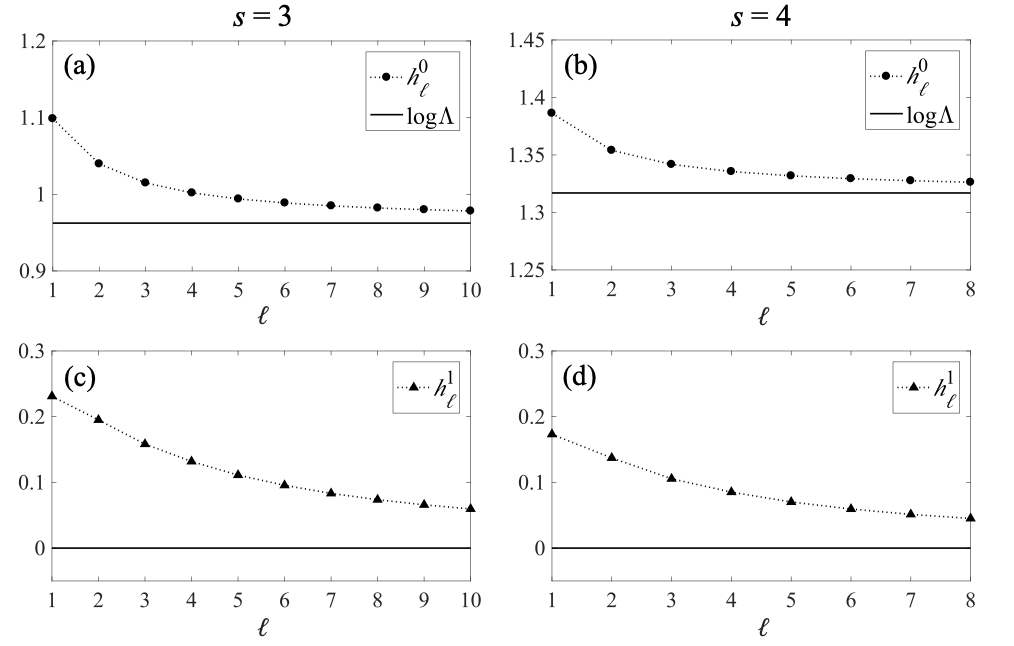
\includegraphics[width=0.85\textwidth]{RJentropy_s3_s4}
        \hspace{0.1\textwidth}
	\caption{\label{fig:RJentropyPlot}
Geometric, $h_\ell^1$, and interior, $h_\ell^0$, parts of entropy vs. the
length $\ell$ of
    a cat map symbol \brick\
for
(a), (c) $s=3$, and
(b), (d) $s=4$.
The interior
    part of entropy
$h_\ell^0$ converges to the exact value of the metric entropy, which is
$\ln(3+\sqrt{5})/2$ for $s=3$ and $\ln(2+\sqrt{3})$ for $s=4$,
respectively.  The geometric part $h_\ell^1$ converges to $0$.
    }
\end{figure}

Since the Lyapunov exponents of {\catlatt} are known explicitly for any
finite lattice, its  metric entropy is known exactly, through the Pesin
entropy formula\rf{Pesin77}. On the other hand, the metric entropy can be
represented through  sums of symbol {\brick s} $\Mm_\R$ measures  in the
limit of growing domain size $|\R|$. As we show below, this connection
can be used to extract the asymptotics of the Jacobian $d(\R)$ which, in
turn, provides the maximum  of measures for symbol {\brick s} in a given
domain $\R$.

\subsection{Cat map entropy}
\label{sect:catEntropy}

Given  measures  $\Msr({b})$ of {\brick s} $ {b}$ of an arbitrary finite
length $\cl{b}=\ell$ one can estimate observables of the dynamical system
with increasing  precision as $\ell$ grows. In the following we apply
this  to estimation of the metric entropy of the cat map.

The metric entropy  of the cat map with respect to measure $\Msr$ can be
represented as the limit
\begin{equation}
h_\Msr =\lim_{{\ell}\to\infty} {h}_\ell,
\label{EntropyEigenvalue}
\end{equation}
where
\[
h_\ell = -\frac{1}{\ell} \sum_{|{b}|=\ell}{\Msr({b}) \log{\Msr({b})}}
\,.
\]
By using the decomposition \refeq{FreqDecomp}, $h_\ell$  can be split as
$h_\ell=h_\ell^{1}+h_\ell^{0}$ into ``geometric'' and ``internal'' parts:
\[
h_\ell^{1}=
-\frac{\sum_{|{b}|=\ell}{|\Pol_{{b}}| \log{|\Pol_{{b}}|}}}{\ell \sum_{|{b}|=\ell}{|\Pol_{{b}}| }},
\qquad
h_\ell^{0}=-\frac{1}{\ell}\log d_\ell
          = \frac{1}{\ell}\log U_{\ell}({s}/{2})
\,.
\]
The ``interior'' part $h_\ell^{0}$ converges to $\log \ExpaEig$ with the
rate $O(1/\ell)$. Since $h_\Msr=\log \ExpaEig$, the cat  map  metric
entropy\rf{Sinai59},  the geometrical part must vanish,
$\lim_{{\ell}\to\infty}h_\ell^{1}=0$. We \edit{illustrate} this numerically for
several values of $s$ in \reffig{fig:RJentropyPlot}. In other words,
metric entropy  is determined solely by the asymptotics of the Jacobian
$d_\ell$.


\subsection{\catLatt\ entropy}
\label{sect:catLattEntropy}

By the linearity of the \catlatt\ automorphism, every \catlatt\
$[\speriod{}\!\times\!\period{}]$ {\twot} has the same spectrum of  the
Lyapunov exponents  $\Lyap_k$, $k=1,\dots,2\speriod{}$, given by the
eigenvalues \refeq{qudreq} $\ExpaEig_k =e^{\Lyap_k}$ of the matrix
$\B_{\scriptscriptstyle L}$.

Accordingly, the map  is fully hyperbolic iff $\edit{2s}=a+b>4$.    In this
case all solutions   of \refeq{qudreq} are paired such that $\Lyap_k^+=
-\Lyap_k^-$ and  $\Lyap_k^+ >0$ for all $k$.  The metric entropy  of
$\Phi_{\speriod{}}$ for a finite $\speriod{}$ is given by the sum of all
positive exponents:
\[
h(\Phi_{\speriod{}})= \sum_{k=1}^\speriod{}  \Lyap_k^+
\,.
\]
 For the   infinite lattice the corresponding  {\spt} entropy of
 $\Phi$ with respect to $\Msr$ is given by  the limit
$
   h_\Msr(\Phi) =\lim_{L\to\infty}\frac{1}{L} {h}(\Phi_{\scriptscriptstyle L})
$.
Alternative, more convenient way to evaluate $h_\Msr(\Phi)$ is to
use numbers $\mathcal{N}_{\speriod{}\period{}}$ of  periodic tori with
spatial-temporal periods $\speriod{},\period{}$, see \refref{GutOsi15,CL18}.
For the linear hyperbolic automorphisms the topological and metric entropies
coincide, leading to
\bea
h_\Msr(\Phi) &=&\lim_{\speriod{},\period{}\to\infty}\frac{1}{LT} \log \mathcal{N}_{\speriod{}\period{}}
\continue
&=&\lim_{\speriod{},\period{}\to\infty}\frac{1}{\speriod{}\period{}} \log \mbox{det} (I-\B_{\speriod{}}^\period{})
=  \lim_{\speriod{},\period{}\to\infty}\frac{1}{\speriod{}\period{}} \log \mbox{det} (I-\B_{\period{}}^\speriod{})
\,.
\label{TopologicalEntropy}
\eea
This yields a closed formula:
\beq
h_\Msr(\Phi)=\frac{1}{\pi^2} \int_0^{\pi}\int_0^{\pi}\,dx\,dy
\log(\edit{2s}-4+4\sin^2 x +4\sin^2 y)
 \,.
\ee{SpatiotemporalEntropy}

Recall that for the (temporal) cat map the constant $d(\R)$  was given
explicitly  by  \refeq{SingleCatJacobian}. In the case of
{\catlatt} we were unable to derive any explicit formula for $d(\R)$.
On the other hand, by the same argument as in the {cat map} case, in the
large domain \R\ limit the asymptotics of $d(\R)$ is determined  by the
metric entropy,
\[
-\lim_{|\R|\to\infty} \frac{1}{|\R|}\log d(\R) =  h_\Msr
\,,
\]
where $h_\Msr$ is the {\spt}  metric entropy \refeq{SpatiotemporalEntropy}
of the {\catlatt}. Therefore, asymptotically we expect
\beq
d(\R) \sim
e^{-|\R| h_\Msr}
\,.
\ee{AsymJacobian}

%%%%%%%%%%%%%%%%%%%%%%%%%%%%%%%%%%%%%%%%%%%%%%%%%%%%%%%%%%%%%%%%%%%%%%%%%%
    \ifsubmission
\section*{References}
    % from ctan.org/tex-archive/biblio/bibtex/contrib/iopart-num/ :
\bibliographystyle{iopart-num}       % APS-like style for physics
\bibliography{../bibtex/siminos}
    \else
\printbibliography[
heading=bibintoc,
title={References}
				  ] %, type=online]  % if not using default "Bibliography"
    \fi

%%%%%%%%%% submission: cut here  %%%%%%%%%%%%%%%%%%%%%%%%%%%
    \ifboyscout
    \clearpage
    % siminos/cats/nonlinTips.tex
% $Author: predrag $ $Date: 2019-10-31 17:06:14 -0400 (Thu, 31 Oct 2019) $

\section{Nonlinearity journal tips}
\label{sect:NonlinTips}

\HREF{https://mc04.manuscriptcentral.com/non} {Author help}

\subsection{Naming your files}

Please name all your files, both figures and text, as follows:
\begin{itemize}
\item Use only characters from the set a to z, A to Z, 0 to 9 and underscore (\_).
\item Do not use spaces or punctuation characters in file names.
\item Do not use any accented characters such as
\'a, \^e, \~n, \"o.
\item Include an extension to indicate the file type (e.g., \verb".tex", \verb".eps", \verb".txt", etc).
\item Use consistent upper and lower case in filenames and in your \LaTeX\ file.
If your \LaTeX\ file contains the line \verb"\includegraphics{fig1.eps}" the figure file must be called
\verb"fig1.eps" and not \verb"Fig1.eps" or \verb"fig1.EPS".  If you are on a Unix system, please ensure that
there are no pairs of figures whose names differ only in capitalization, such as \verb"fig_2a.eps" and \verb"fig_2A.eps",
as Windows systems will be unable to keep the two files in the same directory.
\end{itemize}

\subsection{Preparing your article}

%    \PC{2016-08-18}{
Footnotes should be avoided whenever possible and can often be included
in the text as phrases or sentences in parentheses. If required, they
should be used only for brief notes that do not fit conveniently into the
text. The use of displayed mathematics in footnotes should be avoided
wherever possible and no equations within a footnote should be numbered.
The standard \LaTeX\ macro \verb"\footnote" should be used.  Note that in
\verb"iopart.cls" the \verb"\footnote" command produces footnotes indexed
by a variety of different symbols, whereas in published articles we use
numbered footnotes.  This is not a problem: we will convert
symbol-indexed footnotes to numbered ones during the production process.
%    }

\subsection{The abstract}
The abstract should be self-contained---there should be no references to
figures, tables, equations, bibliographic references etc.

\subsection{Some matters of style}
It will help the readers if your article is written in a clear,
consistent and concise manner. During the production process
we will try to make sure that your work is presented to its
readers in the best possible way without sacrificing the individuality of
your writing.

\begin{enumerate}
\item We recommend using `-ize' spellings (diagonalize,
renormalization, minimization, etc) but there are some common
exceptions to this, for example: devise,
promise and advise.

Do not include `eq.', `equation' etc before an equation number or `ref.'\, `reference' etc before a reference number.
\end{enumerate}

\subsection{Two-line constructions}
For simple fractions in the text the solidus \verb"/", as in
$\lambda/2\pi$, should be used instead of \verb"\frac" or \verb"\over",
using parentheses where necessary to avoid ambiguity,
for example to distinguish between $1/(n-1)$ and $1/n-1$. Exceptions to
this are the proper fractions $\frac12$, $\frac13$, $\frac34$,
etc, which are better left in this form. In displayed equations
horizontal lines are preferable to solidi provided the equation is
kept within a height of two lines. A two-line solidus should be
avoided where possible; the construction $(\ldots)^{-1}$ should be
used instead. For example use:
\begin{equation*}
\frac{1}{M_{\rm a}}\left(\int^\infty_0{\rm d}
\omega\;\frac{|S_o|^2}{N}\right)^{-1}\qquad\mbox{instead of}\qquad
\frac{1}{M_{\rm a}}\biggl/\int^\infty_0{\rm d}
\omega\;\frac{|S_o|^2}{N}.
\end{equation*}

\subsection{Roman and italic in mathematics}
In mathematics mode there are some cases where it is preferable to use a
Roman font; for instance, a Roman d for a differential d, a Roman e for
an exponential e and a Roman i for the square root of $-1$. To
accommodate this and to simplify the  typing of equations,
\verb"iopart.cls" provides some extra definitions. \verb"\rmd",
\verb"\rme" and \verb"\rmi" now give Roman d, e and i respectively for
use in equations, e.g.\ $\rmi x\rme^{2x}\rmd x/\rmd y$ is obtained by
typing \verb"$\rmi x\rme^{2x}\rmd x/\rmd y$".

Certain other common mathematical functions, such as cos, sin, det and
ker, should appear in Roman type. Standard \LaTeX\ provides macros for
most of these functions
(in the cases above, \verb"\cos", \verb"\sin", \verb"\det" and \verb"\ker"
respectively); \verb"iopart.cls" also provides
additional definitions for $\Tr$, $\tr$ and
$\Or$ (\verb"\Tr", \verb"\tr" and \verb"\Or", respectively).

Subscripts and superscripts should be in Roman type if they are labels
rather than variables or characters that take values. For example in the
equation
\[
\epsilon_m=-g\mu_{\rm n}Bm
\]
$m$, the $z$ component of the nuclear spin, is italic because it can have
different values whereas n is Roman because it
is a label meaning nuclear ($\mu_{\rm n}$
is the nuclear magneton).

\subsection{Special characters for mathematics}
Bold italic characters can be used in our journals to signify vectors
(rather than using an upright bold or an over arrow). To obtain this
effect when using \verb"iopart.cls", use \verb"\bi{#1}" within maths
mode, e.g. $\bi{ABCdef}$. Similarly, in \verb"iopart.cls", if upright
bold characters are required in maths, use \verb"\mathbf{#1}" within
maths mode, e.g. $\mathbf{XYZabc}$. The calligraphic (script) uppercase
alphabet is obtained with \verb"\mathcal{AB}" or \verb"\cal{CD}"
($\mathcal{AB}\cal{CD}$).


The package \verb"iopams.sty" uses the definition \verb"\boldsymbol" in \verb"amsbsy.sty"
which allows individual non-alphabetical symbols and Greek letters to be
made bold within equations.
The bold Greek lowercase letters \ifiopams$\balpha \ldots\bomega$,\fi
are obtained with the commands
\verb"\balpha" \dots\ \verb"\bomega" (but note that
bold eta\ifiopams, $\bfeta$,\fi\ is \verb"\bfeta" rather than \verb"\beta")
and the capitals\ifiopams, $\bGamma\ldots\bOmega$,\fi\ with commands
\verb"\bGamma" \dots\
\verb"\bOmega". Bold versions of the following symbols are
predefined in \verb"iopams.sty":
bold partial\ifiopams, $\bpartial$,\fi\ \verb"\bpartial",
bold `ell'\ifiopams, $\bell$,\fi\  \verb"\bell",
bold imath\ifiopams, $\bimath$,\fi\  \verb"\bimath",
bold jmath\ifiopams, $\bjmath$,\fi\  \verb"\bjmath",
bold infinity\ifiopams, $\binfty$,\fi\ \verb"\binfty",
bold nabla\ifiopams, $\bnabla$,\fi\ \verb"\bnabla",
bold centred dot\ifiopams, $\bdot$,\fi\  \verb"\bdot". Other
characters are made bold using
\verb"\boldsymbol{\symbolname}".

\begin{table}
\caption{\label{math-tab2}Other macros defined in {\tt iopart.cls} for use in maths.}
\begin{tabular*}{\textwidth}{@{}l*{15}{@{\extracolsep{0pt plus
12pt}}l}}
\br
Macro&Result&Description\\
\mr
\verb"\fl"&&Start line of equation full left\\
\verb"\case{#1}{#2}"&$\case{\#1}{\#2}$&Text style fraction in display\\
\verb"\Tr"&$\Tr$&Roman Tr (Trace)\\
\verb"\tr"&$\tr$&Roman tr (trace)\\
\verb"\Or"&$\Or$&Roman O (of order of)\\
\verb"\lshad"&$\lshad$&Text size left shadow bracket\\
\verb"\rshad"&$\rshad$&Text size right shadow bracket\\
\br
\end{tabular*}
\end{table}

\subsection{Alignment of displayed equations}

The \verb"iopart.cls" class file aligns left and indents each line of a
display.  To make any line start at the left margin of the page, add
\verb"\fl" at start of the line (to indicate full left).

Using the \verb"eqnarray" environment equations will naturally be aligned
left and indented without the use of any ampersands for alignment, see
equations (\ref{eq1}) and (\ref{eq2})
\begin{eqnarray}
\alpha + \beta =\gamma^2, \label{eq1}\\
\alpha^2 + 2\gamma + \cos\theta = \delta. \label{eq2}
\end{eqnarray}

Where some secondary alignment is needed, for instance a second part of
an equation on a second line, a single ampersand is added at the point of
alignment in each line  (see  (\ref{eq3}) and (\ref{eq4})).
\begin{eqnarray}
\alpha &=2\gamma^2 + \cos\theta + \frac{XY \sin\theta}{X+ Y\cos\theta} \label{eq3}\\
 & = \delta\theta PQ \cos\gamma. \label{eq4}
\end{eqnarray}

Two points of alignment are possible using two ampersands for alignment
(see  (\ref{eq5}) and (\ref{eq6})).  Note in this case extra space
\verb"\qquad" is added before the second ampersand in the longest line
(the top one) to separate the condition from the equation.
\begin{eqnarray}
\alpha &=2\gamma^2 + \cos\theta + \frac{XY \sin\theta}{X+ Y\cos\theta}\qquad& \theta > 1 \label{eq5}\\
 & = \delta\theta PQ \cos\gamma &\theta \leq 1.\label{eq6}
\end{eqnarray}

For a long equation which has to be split over more than one line the
first line should start at the left margin, this is achieved by inserting
\verb"\fl" (full left) at the start of the line. The use of the alignment
parameter \verb"&" is not necessary unless some secondary alignment is
needed.
\begin{eqnarray}
\fl \alpha + 2\gamma^2 = \cos\theta + \frac{XY \sin\theta}{X+ Y\cos\theta} +  \frac{XY \sin\theta}{X- Y\cos\theta} +
+ \left(\frac{XY \sin\theta}{X+ Y\cos\theta}\right)^2 \nonumber\\
+  \left(\frac{XY \sin\theta}{X- Y\cos\theta}\right)^2.\label{eq7}
\end{eqnarray}

The plain \TeX\ command \verb"\eqalign" can be used within an
\verb"equation" environment to obtain a multiline equation with a single
centred number, for example
\begin{equation}
\eqalign{\alpha + \beta =\gamma^2 \cr
\alpha^2 + 2\gamma + \cos\theta = \delta.}
\end{equation}

\subsection{Miscellaneous}

Exponential expressions, especially those containing subscripts or
superscripts, are clearer if the notation $\exp(\ldots)$ is used, except for
simple examples. For instance $\exp[\rmi(kx-\omega t)]$ and $\exp(z^2)$ are
preferred to $\e^{\rmi(kx-\omega t)}$ and $\e^{z^2}$, but
$\e^x$
is acceptable.

The square root sign $\sqrt{\phantom{b}}$ should
only be used with relatively
simple expressions, e.g.\ $\sqrt2$ and $\sqrt{a^2+b^2}$;
in other cases the
power $1/2$ should be used; for example, $[(x^2+y^2)/xy(x-y)]^{1/2}$.

It is important to distinguish between $\ln = \log_\e$ and $\lg
=\log_{10}$. Braces, brackets and parentheses should be used in the
following order: $\{[(\;)]\}$.

Decimal fractions should always be preceded by a zero: for example 0.123
{\bf not} .123. For long numbers use thin spaces after every third
character away from the position of the decimal point, unless this leaves
a single separated character: e.g.\ $60\,000$, $0.123\,456\,78$ but 4321
and 0.7325.

Equations should be followed by a full stop (periods) when at the end
of a sentence.

\subsection{Equation numbering and layout in {\tt iopart.cls}}
\label{eqnum}

If the command \verb"\eqnobysec" is included in the preamble, equation
numbering by section is obtained, e.g.\ (2.1), (2.2), etc.
Refer to equations in the text using the
equation number in parentheses. It is not normally necessary to include
the word equation before the number; and abbreviations such as eqn or eq
should not be used. In \verb"iopart.cls", there are alternatives to the
standard \verb"\ref" command that you might find useful---see
\tref{abrefs}.

Sometimes it is useful to number equations as parts of the same
basic equation. This can be accomplished in \verb"iopart.cls" by inserting the
commands \verb"\numparts" before the equations concerned and
\verb"\endnumparts" when reverting to the normal sequential numbering.
For example using \verb"\numparts \begin{eqnarray}" ... \verb"\end{eqnarray} \endnumparts":

\numparts
\begin{eqnarray}
T_{11}&=(1+P_\e)I_{\uparrow\uparrow}-(1-P_\e)
I_{\uparrow\downarrow},\label{second}\\
T_{-1-1}&=(1+P_\e)I_{\downarrow\downarrow}-(1-P_\e)I_{\uparrow\downarrow},\\
S_{11}&=(3+P_\e)I_{\downarrow\uparrow}-(3-P_e)I_{\uparrow\uparrow},\\
S_{-1-1}&=(3+P_\e)I_{\uparrow\downarrow}-(3-P_\e)
I_{\downarrow\downarrow}.
\end{eqnarray}
\endnumparts

Equation labels within the \verb"\eqnarray" environment will be referenced
as subequations, e.g. (\ref{second}).

\subsection{Miscellaneous extra commands for displayed equations}
The \verb"\cases" command has been amended slightly in \verb"iopart.cls" to
increase the space between the equation and the condition.
\Eref{cases}
demonstrates simply the output from the \verb"\cases" command
\begin{equation}
\label{cases}
X=\cases{1&for $x \ge 0$\\
-1&for $x<0$\\}
\end{equation}
%The code used was:
%\small\begin{verbatim}
%\begin{equation}
%\label{cases}
%X=\cases{1&for $x \ge 0$\\
%-1&for $x<0$\\}
%\end{equation}
%\end{verbatim}
%\normalsize

To obtain text style fractions within displayed maths the command
\verb"\case{#1}{#2}" can be used instead
of the usual \verb"\frac{#1}{#2}" command or \verb"{#1 \over #2}".

When two or more short equations are on the same line they should be
separated by a `qquad space' (\verb"\qquad"), rather than
\verb"\quad" or any combination of \verb"\,", \verb"\>", \verb"\;"
and \verb"\ ".

\subsection{Preprint references}
Preprints may be referenced but if the article concerned has been
published in a peer-reviewed journal, that reference should take
precedence. If only a preprint reference can be given, it is helpful to
include the article title. Examples are:
\vskip6pt
\numrefs{1}
\item Neilson D and Choptuik M 2000 {\it Class. Quantum Grav.} {\bf 17}
        761 (arXiv:gr-qc/9812053)
\item Sundu H, Azizi K, S\"ung\"u J Y and Yinelek N 2013
        Properties of $D_{s2}^*(2573)$ charmed-strange tensor meson
        arXiv:1307.6058
\endnumrefs


\subsection{Cross-referencing\label{xrefs}}

\verb"label" may contain letters, numbers
or punctuation characters but must not contain spaces or commas. It is also
recommended that the underscore character \_{} is not used in cross
referencing.

Thus labels of the form \verb"eq:partial", \verb"fig:run1",
\verb"eq:dy'", etc, may be used. When several references occur together
in the text \verb"\cite" may be used with multiple labels with commas but
no spaces separating them; the output will be the numbers within a single
pair of square brackets with a comma and a thin space separating the
numbers. Thus \verb"\cite{label1,label2,label4}" would give [1,\,2,\,4].
Note that no attempt is made by the style file to sort the labels and no
shortening of groups of consecutive numbers is done. Authors should
therefore either try to use multiple labels in the correct order, or use
a package such as \verb"cite.sty" that reorders labels correctly.


\Table{\label{abrefs}
Alternatives to the normal references command {\tt $\backslash$ref}
available in {\tt iopart.cls}, and the text generated by them. Note it is
not normally necessary to include the word equation before an equation
number except where the number starts a sentence. The versions producing
an initial capital should only be used at the start of sentences.}
\br
Reference&Text produced\\
\mr
\verb"\eref{<label>}"&(\verb"<num>")\\
\verb"\Eref{<label>}"&Equation (\verb"<num>")\\
\verb"\fref{<label>}"&figure \verb"<num>"\\
\verb"\Fref{<label>}"&Figure \verb"<num>"\\
\verb"\sref{<label>}"&section \verb"<num>"\\
\verb"\Sref{<label>}"&Section \verb"<num>"\\
\verb"\tref{<label>}"&table \verb"<num>"\\
\verb"\Tref{<label>}"&Table \verb"<num>"\\
\br
\endTable

\subsection{Tables and table captions}
Tables are numbered serially and referred to in the text
by number (table 1, etc, {\bf not} tab. 1). Each table should have an
explanatory caption which should be as concise as possible. If a table
is divided into parts these should be labelled \pt(a), \pt(b),
\pt(c), etc but there should be only one caption for the whole
table, not separate ones for each part.

The standard form for a table in \verb"iopart.cls" is:
\small\begin{verbatim}
\begin{table}
\caption{\label{label}Table caption.}
\begin{indented}
\item[]\begin{tabular}{@{}llll}
\br
Head 1&Head 2&Head 3&Head 4\\
\mr
1.1&1.2&1.3&1.4\\
2.1&2.2&2.3&2.4\\
\br
\end{tabular}
\end{indented}
\end{table}
\end{verbatim}\normalsize

\begin{enumerate}
\item The caption comes before the table. It should have a period at
the end.

\item Tables are normally set in a smaller type than the text.
The normal style is for tables to be indented. This is accomplished
by using \verb"\begin{indented}" \dots\ \verb"\end{indented}"
and putting \verb"\item[]" before the start of the tabular environment.
Omit these
commands for any tables which will not fit on the page when indented.

\item The default is for columns to be aligned left and
adding \verb"@{}" omits the extra space before the first column.

\item Tables have only horizontal rules and no vertical ones. The rules at
the top and bottom are thicker than internal rules and are set with
\verb"\br" (bold rule).
The rule separating the headings from the entries is set with
\verb"\mr" (medium rule).  These are special \verb"iopart.cls" commands.

\item Numbers in columns should be aligned on the decimal point;
to help do this a control sequence \verb"\lineup" has been defined
in \verb"iopart.cls"
which sets \verb"\0" equal to a space the size of a digit, \verb"\m"
to be a space the width of a minus sign, and \verb"\-" to be a left
overlapping minus sign. \verb"\-" is for use in text mode while the other
two commands may be used in maths or text.
(\verb"\lineup" should only be used within a table
environment after the caption so that \verb"\-" has its normal meaning
elsewhere.) See table~\ref{tabone} for an example of a table where
\verb"\lineup" has been used.
\end{enumerate}

\begin{table}
\caption{\label{tabone}A simple example produced using the standard table commands
and $\backslash${\tt lineup} to assist in aligning columns on the
decimal point. The width of the
table and rules is set automatically by the
preamble.}

\begin{indented}
\lineup
\item[]\begin{tabular}{@{}*{7}{l}}
\br
$\0\0A$&$B$&$C$&\m$D$&\m$E$&$F$&$\0G$\cr
\mr
\0\023.5&60  &0.53&$-20.2$&$-0.22$ &\01.7&\014.5\cr
\0\039.7&\-60&0.74&$-51.9$&$-0.208$&47.2 &146\cr
\0123.7 &\00 &0.75&$-57.2$&\m---   &---  &---\cr
3241.56 &60  &0.60&$-48.1$&$-0.29$ &41   &\015\cr
\br
\end{tabular}
\end{indented}
\end{table}

\subsection{Simplified coding and extra features for tables}
The basic coding format can be simplified using extra commands provided in
the \verb"iopart" class file. The commands up to and including
the start of the tabular environment
can be replaced by
\small\begin{verbatim}
\Table{\label{label}Table caption}
\end{verbatim}\normalsize
and this also activates the definitions within \verb"\lineup".
The final three lines can also be reduced to \verb"\endTable" or
\verb"\endtab". Similarly for a table which does not fit on the page when indented
\verb"\fulltable{\label{label}caption}" \dots\ \verb"\endfulltable"
can be used. \LaTeX\ optional positional parameters can, if desired, be added after
\verb"\Table{\label{label}caption}" and \verb"\fulltable{\label{label}caption}".


\verb"\centre{#1}{#2}" can be used to centre a heading
\verb"#2" over \verb"#1"
columns and \verb"\crule{#1}" puts a rule across
\verb"#1" columns. A negative
space \verb"\ns" is usually useful to reduce the space between a centred
heading and a centred rule. \verb"\ns" should occur immediately after the
\verb"\\" of the row containing the centred heading (see code for
\tref{tabl3}). A small space can be
inserted between rows of the table
with \verb"\ms" and a half line space with \verb"\bs"
(both must follow a \verb"\\" but should not have a
\verb"\\" following them).

\Table{\label{tabl3}A table with headings spanning two columns and containing notes.
To improve the
visual effect a negative skip ($\backslash${\tt ns})
has been put in between the lines of the
headings. Commands set-up by $\backslash${\tt lineup} are used to aid
alignment in columns. $\backslash${\tt lineup} is defined within
the $\backslash${\tt Table} definition.}
\br
&&&\centre{2}{Separation energies}\\
\ns
&Thickness&&\crule{2}\\
Nucleus&(mg\,cm$^{-2}$)&Composition&$\gamma$, n (MeV)&$\gamma$, 2n (MeV)\\
\mr
$^{181}$Ta&$19.3\0\pm 0.1^{\rm a}$&Natural&7.6&14.2\\
$^{208}$Pb&$\03.8\0\pm 0.8^{\rm b}$&99\%\ enriched&7.4&14.1\\
$^{209}$Bi&$\02.86\pm 0.01^{\rm b}$&Natural&7.5&14.4\\
\br
\end{tabular}
\item[] $^{\rm a}$ Self-supporting.
\item[] $^{\rm b}$ Deposited over Al backing.
\end{indented}
\end{table}

Units should not normally be given within the body of a table but
given in brackets following the column heading; however, they can be
included in the caption for long column headings or complicated units.
Where possible tables should not be broken over pages.
If a table has related notes these should appear directly below the table
rather than at the bottom of the page. Notes can be designated with
footnote symbols (preferable when there are only a few notes) or
superscripted small roman letters. The notes are set to the same width as
the table and in normal tables follow after \verb"\end{tabular}", each
note preceded by \verb"\item[]". For a full width table \verb"\noindent"
should precede the note rather than \verb"\item[]". To simplify the coding
\verb"\tabnotes" can, if desired, replace \verb"\end{tabular}" and
\verb"\endtabnotes" replaces
\verb"\end{indented}\end{table}".

\subsection{Inclusion of graphics files\label{figinc}}

Below each figure should be a brief caption describing it and, if
necessary, interpreting the various lines and symbols on the figure.
As much lettering as possible should be removed from the figure itself
and included in the caption. If a figure has parts, these should be
labelled ($a$), ($b$), ($c$), etc and all parts should be described
within a single caption. \Tref{blobs} gives the definitions for describing
symbols and lines often used within figure captions (more symbols are
available when using the optional packages loading the AMS extension fonts).

\subsection{Supplementary Data}

Supplementary data
enhancements typically consist of video clips, animations or
data files, tables of extra information or extra figures. See
guidelines on supplementary data file formats,
`Author Guidelines' link at \verb"http://authors.iop.org".

Software, in the form of input scripts for mathematical packages (such as
Mathematica notebook files), or source code that can be interpreted or
compiled (such as Python scripts or Fortran or C programs), or executable
files, can sometimes be accepted as supplementary data, but the journal
may ask you for assurances about the software and distribute them from
the article web page only subject to a disclaimer.  Contact the journal
in the first instance if you want to submit software.

\begin{table}[t]
\caption{\label{blobs}Control sequences to describe lines and symbols in figure
captions.}
\begin{indented}
\item[]\begin{tabular}{@{}lllll}
\br
Control sequence&Output&&Control sequence&Output\\
\mr
\verb"\dotted"&\dotted        &&\verb"\opencircle"&\opencircle\\
\verb"\dashed"&\dashed        &&\verb"\opentriangle"&\opentriangle\\
\verb"\broken"&\broken&&\verb"\opentriangledown"&\opentriangledown\\
\verb"\longbroken"&\longbroken&&\verb"\fullsquare"&\fullsquare\\
\verb"\chain"&\chain          &&\verb"\opensquare"&\opensquare\\
\verb"\dashddot"&\dashddot    &&\verb"\fullcircle"&\fullcircle\\
\verb"\full"&\full            &&\verb"\opendiamond"&\opendiamond\\
\br
\end{tabular}
\end{indented}
\end{table}




\begin{table}
\caption{Macros defined within {\tt iopart.cls}
for use with figures and tables.}
\begin{indented}
\item[]\begin{tabular}{@{}l*{15}{l}}
\br
Macro name&Purpose\\
\mr
\verb"\Figures"&Heading for list of figure captions\\
\verb"\Figure{#1}"&Figure caption\\
\verb"\Tables"&Heading for tables and table captions\\
\verb"\Table{#1}"&Table caption\\
\verb"\fulltable{#1}"&Table caption for full width table\\
\verb"\endTable"&End of table created with \verb"\Table"\\
\verb"\endfulltab"&End of table created with \verb"\fulltable"\\
\verb"\endtab"&End of table\\
\verb"\br"&Bold rule for tables\\
\verb"\mr"&Medium rule for tables\\
\verb"\ns"&Small negative space for use in table\\
\verb"\centre{#1}{#2}"&Centre heading over columns\\
\verb"\crule{#1}"&Centre rule over columns\\
\verb"\lineup"&Set macros for alignment in columns\\
\verb"\m"&Space equal to width of minus sign\\
\verb"\-"&Left overhanging minus sign\\
\verb"\0"&Space equal to width of a digit\\
\br
\end{tabular}
\end{indented}
\end{table}


    \clearpage
    % siminos/spatiotemp/chapter/GHJSC16blog.tex
% $Author: predrag $ $Date: 2021-12-24 01:25:20 -0500 (Fri, 24 Dec 2021) $

\section{Cats' GHJSC16blog}
\label{sect:GHJSC16blog}

Internal discussions of \refref{GHJSC16} edits:
Move good text not used in \refref{GHJSC16} to this file, for possible
reuse later.

%%%%%%%%%%%%%%%%%%%%%%%%%%%%%%%%%%%%%%%%%%%%%%%%%%%%%%%%%%%%%%%%%%%%%%%
\begin{description}

\item[2016-12-06 Boris] I prefer a precise title.  E.g. :
\\ {\em Linear encoding of cat map lattices}

Some earlier titles:
\\ {\em Linear encoding of the \catlatt} %PC 2016-11-27
\\ {\em A \catlatt\ encoded} %PC 2016-11-27
\\ {\em A spatiotemporal code for a coupled maps lattice} %PC 2016-11-27
\\ {\em A spatiotemporal symbolic dynamics for a coupled maps lattice} %PC 2016-11-27
\\ {\em A spatiotemporal symbolic dynamics for a coupled cat maps lattice} %PC 2016-11-14
\\ {\em A linear symbolic dynamics for coupled cat maps lattices}
\\ {\em A  spatiotemporal herding of coupled lattice cats}
\\ {\em Herding five cats}           % PC internal

\item[2016-11-18 Predrag]
A theory of turbulence that has done away with \emph{dynamics}?
We rest our case.

\item[2016-10-05 Predrag]
My approach is that this is written for field theorists, fluid dynamicists
etc., who do not see any reason to look at cat maps, so I am trying to be
pedagogical, motivate it as that chaotic counterpart of the harmonic
oscillator, something that field theorists fell comfortable with (they should
not, but they do).

\item[2016-11-13 Predrag]
The next thing to rethink: Green's functions for periodic lattices are in
ChaosBook sections D.3 Lattice derivatives and on, for the Hermitian
Laplacian and $s=2$. For real $s>2$ cat map, the potential is inverted
harmonic oscillator, the frequency is imaginary (Schr\"odinger in
imaginary time), eigenvectors real - should
be a straightforward generalization. Have done this already while studying
Ornstein-Uhlenbeck with Lippolis and Henninger - the eigenfunctions are
Hermite polynomials times Gaussians.


\item[2016-11-13 Predrag]
The claim
``the cat map
\(
{A} =\left(\begin{array}{cc}
 a & c \\
 d & b
  \end{array} \right )
\)
is assumed to be time-reversal invariant, i.e. $c = d$.''
seems to be in conflict with Boris choice
\(
A = \left (
\begin{array}{cc}
s-1 & 1 \\
s-2 & 1 \\
\end{array}
    \right )
\)


We write \refeq{OneCat} as
\begin{equation}
(\Box +2 - s)x_{t} =\Ssym{t}
%    \,,  \qquad
% \Box\,x_{t}:= x_{t-1}-2x_{t} +x_{t+1}
\,,
\label{OneCatBl}
\end{equation}
Percival and Vivaldi\rf{PerViv} write their Eq.~(3.6)
\beq
(\Box +2 - s) x_{t} = -b_t
\ee{PerViv3.6Bl}
so their ``stabilising impulses'' $b_t$ (defined on interval
$x\in[-1/2,1/2)$) have the opposite sign to our ``winding numbers'' $\Ssym{t}$
(defined on $\ssp\in[0,1)$).

Did not replace Arnol'd
by PerViv choice.
\beq
A = \left (
\begin{array}{cc}
0 & 1 \\
-1 & s \\
\end{array}
\right )
\,,
% \qquad\det A= 1 \,,
\ee{PerViv2.10b}

\bea
 x_{t+1} &=&  p_t            \quad \mod 1
    \continue
 p_{t+1} &=& -x_t +  s\,p_t               \quad \mod 1
\label{eq:CatMapPspace1}
\eea

Predrag's formula, removed by Boris 2017-01-15:
\bea
\begin{array}{ccl}
  x_{t+1} &=& (s-1)\,x_t + p_t     \\
  p_{t+1} &=& (s-2)\,x_t + p_t
\end{array}
            \quad \mod 1
\,,
\label{eq:CatMapPspace}
\eea

Predrag's formula, removed by Boris 2017-01-15:
\\
 As the 3-point
discretization of the second time derivative ${d^2}/{dt^2}$
(central difference operator) is
\(
\Box\, \ssp_t \equiv \ssp_{t+1} - 2\ssp_{t} + \ssp_{t-1}
\)
(with the time step set to $\Delta t= 1$), the {\em temporal} cat map
\refeq{eq:CatMapIntr} can be rewritten as the discrete time Newton equation
for inverted harmonic potential,
\beq
(\Box +2 - s)\, \ssp_{t} = \Ssym{t}
\,.
\ee{eq:CatMapNewton}

Predrag's formula, replaced by a more abstract form by Boris 2017-01-15:
\\
a $d$\dmn\ {\spt} pattern
\(
\{\ssp_{z}\} = \{\ssp_{n_1 n_2 \cdots n_d}\}
\)
requires {\em $d$\dmn} {\spt} {\brick}
\(
\{\m_{z}\} = \{\m_{n_1 n_2 \cdots n_d}\}
\,,
\)

for
definiteness written as
\beq
A = \left (
\begin{array}{cc}
2 & 1 \\
1 & 1 \\
\end{array}
\right )
\,,
% \qquad\det A= 1 \,,
\ee{ArnoldCat1}

\item[2016-08-20 Predrag]
``
The fact that even Dyson\rf{DysFal92} counts cat map periods should give
us pause - clearly, some nontrivial number theory is afoot.
''

Not sure whether this is related to cat map symbolic dynamics that we use,
    dropped for now: ``
Problems with the discretization of Arnol'd cat map were pointed out in
\refrefs{Blank97,BlaKel98}. \refRef{BlaKel98} discusses two partitions of
the cat map unit square.
    ''

``
and resist the
siren song of the Hecke operators\rf{KurRud00,Mezzadri02}
''
\bigskip


While stability multipliers depend only on the trace $s$, the \statesp\
eigenvectors depend on the explicit matrix $A$, and so do ``winding numbers''
$\Ssym{t}$ (which also depend on the defining interval $x\in[-1/2,1/2)$, Percival
and Predrag choice, or Boris choice $x\in[0,1)$.
Time-reversed has different eigenvectors (orthogonal to the forward-time
ones), so I am not even sure how time reversed $\Ssym{t}$ look.

\item[2016-05-21 Predrag]
Behrends\rf{Behrends98,BehFie98} {\em The ghosts of the cat} is fun - he
uncovers various regular patterns in the iterates of the cat map.

\item[2016-09-27 Boris]
{\bf Cat maps and \catlatt s}

In the {\catlatt}, ``particles'' (\ie, a cat map at each  periodic lattice
site) are coupled by the next-neighbor coupling rules:
\[
q_{n, t+1}=p_{nt}+(s-1)q_{nt} - q_{n+1,t} - q_{n-1,t} - {m}^q_{n,t+1}
\]
\[
p_{n,t+1}= p_{nt} + (s-2) q_{nt} - q_{n+1,t} - q_{n-1,t} - {m}^p_{n,t+1}
\]
The symbols of interest can be found by:
\[
\Ssym{nt} = q_{n,t+1} + q_{n,t-1} + q_{n+1,t} + q_{n-1, t} -  s \, q_{nt}
\,.
\]

\item[2016-10-27 Boris]
Gutkin and Osipov\rf{GutOsi15} write:
``In general, calculating periodic orbits of a  non-integrable  system  is a
non-trivial  task.   To  this  end  a  number  of  methods have  been
developed,'' and then,  for a mysterious reasons, they refer to
\refref{baranger88}.

%\item[2016-10-27 Boris]
%Added to \refsect{sect:twots} the following  references:
%M. Sieber and K. Richter\rf{SieRic01},
%S. M\"uller, S. Heusler, P. Braun, F. Haake and A. Altland\rf{MuHeBrHaAl04},
%B. Gutkin, V.Al. Osipov\rf{GutOsi13a},
%B.~Gutkin, V.Al.~Osipov\rf{GutOsi13} (Predrag added \refref{GutOsi15} as well).

%%%%%%%%%%%%%%%%%%%%%%%%%%%%%%%%%%%%%%%%%%%%%%%%%%%%%%%%%%%%%%%%%%%%%%%%
\item[2016-11-07 Predrag]

The dynamical systems literature tends to focus on \emph{local} problems:
bifurcations of a single time-invariant solution (\eqv, \reqv, \po\ or
\rpo) in low\dmn\ settings (3-5 coupled ODEs, 1\dmn\\ PDE).
The problem that we face is \emph{global}: organizing and relating
\emph{simultaneously} infinities of unstable \rpo s in
$\infty$\dmn\ state spaces, orbits that are presumed to form the
skeleton of turbulence (see \refref{GibsonMovies} for a gentle
introduction) and are typically not solutions that possess the symmetries
of the problem. In this quest we found the standard equivariant
bifurcation theory literature not very helpful, as its general focus is
on bifurcations of solutions, which admit all or some of the symmetries
of the problem at hand.
%%%%%%%%%%%%%%%%%%%%%%%%%%%%%%%%%%%%%%%%%%%%%%%%%%%%%%%%%%%%%%%%%%%%%%%%

%%%%%%%%%%%%%%%%%%%%%%%%%%%%%%%%%%%%%%%%%%%%%%%%%%%%%%%%%%%%%%%%%%%%%%%%
\item[2016-11-17 Predrag]
Adler and Weiss\rf{AdWei67} discovered that certain  mappings  from  the
torus  to  itself,  called hyperbolic  toral  automorphisms have  Markov
partitions,  and  in  fact  these  partitions  are  parallelograms. One
famous example is the Arnol'd Cat Map

(Axiom A; Anosov)

are a family of analytic hyperbolic
automorphisms of the  2\dmn\  torus which

The ``linear code'' was introduced and worked out in detail in
influential papers of Percival and Vivaldi\rf{PerViv,BirViv,PerViv87b}.

For $d=1$ lattice, $s=5$ the spatial period 1 fixed point is
equivalent to the usual $s=3$ Arnol'd cat map.

The cat map partitions the \statesp\ into $|\A|$ regions, with borders defined
by the condition that the two adjacent labels $k,k+1$ simultaneously satisfy
\refeq{OneCat},
\beq
\ssp_{1} -s\ssp_{0} + \ssp_{-1} - \epsilon =k
\,,
\ee{OneCat1}
\beq
\ssp_{1} -s\ssp_{0} + \ssp_{-1} + \epsilon =k+1
\,,
\ee{OneCat2}
\beq
\ssp_{2} -s\ssp_{1} + \ssp_{0}=\Ssym{1}
\,,
\ee{OneCat3}
\beq
\ssp_{1} -s\ssp_{0} + \ssp_{-1} =\Ssym{0}
\,,
\ee{OneCat4}

\[
  (\ssp_{0},\ssp_{1}) = (0,0) \to (0,0)
  \,,\quad
  (1,0) \to (0,-1)
  \,,\quad
  (0,1) \to (1,s)
  \,,\quad
  (1,1) \to (1,s-1)
\]


%%%%%%%%%%%%%%%%%%%%%%%%%%%%%%%%%%%%%%%%%%%%%%%%%%%%%%%%%%%%%%%%%%%%%%%%

\item[2016-11-05 Predrag] Dropped this:
\\
Note the two  symmetries of the dynamics\rf{Keating91a}:
%
%\subsection{Cat maps and their symmetries}
%\label{sect:catMsymms}
%
The calculations generalize directly to any cat map invariant
under time reversal\rf{KeaMez00}.

\item[2016-11-11 Boris]
{\bf ``Deeper insight'' into $d=2$ symbolic dynamics}
Information comes locally (both in space and time). Allows to understand
correlations between {\twots}. Connection with field theories.

%\BG{2016-10-21}{
To Predrag: we have  similar results on $2\times 1$ \brick s, but I think
$1\times 1$,  $2\times 2$ is enough. Agree?\\
{\bf 2016-12-08 Predrag}: I agree
%                }

\item[2016-12-06 Boris] Confused about Predrag's claim that
\refrefs{Christiansen97,GHCW07} tile `` spatially and temporally infinite
domains''(?) In both papers the spatial extension of the system  is finite,
and the attractors have relatively small dimensions.
\\
{\bf 2016-12-08 Predrag}: I rewrote that now, is it clearer?

\item[2016-12-06 Boris] Is this claim true:
``Temporally chaotic systems are exponentially unstable with time: double the
time, and roughly twice as many \po s are required to describe it to the same
accuracy.  For large spatial extents, the complexity of
the spatial shapes also needs to be taken into account. A {\spt}ly
chaotic system is \emph{extensive} in the sense that ...''
Double the time and the number of \po s is  squared?
\\
{\bf 2016-12-08 Predrag}: It is true only for discrete time, complete binary
dynamics, but any other statement brings in more confusing words. I do not
want to say ``entropy'' here. I rewrote
it now.

\item[2016-12-06 Boris] Predrag's statement
``Essentially, as the stretching is uniform, distinct admissible symbol
patterns count all patterns of a given size, and that can be accomplished by
construction the appropriate finite size transition matrices\rf{CBcount}.''
is true only for symbolic dynamics based on Markov partitions. Wrong e.g.,
for linear coding.
\\
{\bf 2016-12-08 Predrag}: I rewrote that now, is it correct?

\item[2016-12-12 Predrag] My claim (in a conversation with Boris) that
\catlatt\ symbolic dynamics is ``$d$\dmn'' was nonsensical. I have now removed
this from the draft: ``
The key
innovation of \refref{GutOsi15} is the realization (an insight that applies
to all coupled-map lattices, and all PDEs modeled by them, not only the
system considered here) that $d$\dmn\ {\spt} orbit $\{x_{z}\}$
requires {\em $d$\dmn} symbolic dynamics code
\(
\{\m_{z}\} = \{(\m_{1},\m_{2},\cdots,\m_{d})\}
\,,
\)
rather than a \emph{single} temporal symbol sequence (as one is tempted to do
when describing a finite coupled $N^{d-1}$-``particle'' system).''

%%%%%%%%%%%%%%%%%%%%%%%%%%%%%%%%%%%%%%%%%%%%%%%%%%%%%%%%%%%%%%%%%%
\begin{figure}
	\centering
[the same plot as \reffig{fig:SingleCatPartit}]
	\caption{\label{fig:SingleCat1color}
(Color online)
Newtonian Arnol'd cat map $(\ssp_{0},\ssp_{1})$  \statesp\ partition into
(a) 4 regions labeled by $\Ssym{0}.$ , obtained from
$(\ssp_{-1},\ssp_{0})$ \statesp\ by one iteration (the same as
\reffig{fig:CatMapStatesp}).
(b) 14 regions labeled by past {\brick} $\Ssym{-1}\Ssym{0}.$ , obtained from
$(\ssp_{-2},\ssp_{-1})$ \statesp\ by two iterations.
(c) 44 regions, past {\brick} $\Ssym{-2}\Ssym{-1}\Ssym{0}.$
(d) 4 regions labeled by $.\Ssym{1}$ , obtained from
$(\ssp_{2},\ssp_{1})$ \statesp\ by one backward iteration.
(e) 14 regions labeled by future {\brick} $.\Ssym{1}\Ssym{2}$ , obtained from
$(\ssp_{3},\ssp_{2})$ \statesp\ by two backward iterations.
(f) 44 regions, future {\brick} $\Ssym{3}\Ssym{2}\Ssym{1}.$
Each color has the same total area ($1/6$ for $\Ssym{t} = \underline{1},
2$, and $1/3$ for $\Ssym{t} = 0, 1$). All boundaries are straight
lines with rational slopes.
% while the slopes tend to irrational values set by
% stable/unstable directions of the cat map exponentially fast in the limit $t
% \rightarrow \pm\infty$.
	}
\end{figure}
%%%%%%%%%%%%%%%%%%%%%%%%%%%%%%%%%%%%%%%%%%%%%%%%%%%%%%%%%%%%%%%%%%

%%%%%%%%%%%%%%%%%%%%%%%%%%%%%%%%%%%%%%%%%%%%%%%%%%%%%%%%%%%%%%%%%%
\begin{figure}
	\centering
[the same plot as \reffig{fig:SingleCatPartit}]
	\caption{\label{fig:SingleCatBW}
Newtonian Arnol'd cat map $(\ssp_{0},\ssp_{1})$  \statesp\ partition into
(a) 14 regions labeled by {\brick} $b = \Ssym{0}.\Ssym{1}$, the
intersection of one past (\reffig{fig:SingleCat1color}\,(a)) and
one future iteration (\reffig{fig:SingleCat1color}\,(d)).
(b) {\brick} $b = \Ssym{-1}\Ssym{0}.\Ssym{1}$, the
intersection of two past (\reffig{fig:SingleCat1color}\,(b)) and
one future iteration (\reffig{fig:SingleCat1color}\,(d)).
(c) {\brick} $b = \Ssym{-1}\Ssym{0}.\Ssym{1}\Ssym{2}$, the
intersection of two past (\reffig{fig:SingleCat1color}\,(b)) and
two future iterations (\reffig{fig:SingleCat1color}\,(e)).
Note that while some regions involving external alphabet (such as
\prune{22} in (a)) are pruned, the interior alphabet labels a horseshoe,
indicated by the shaded regions.
Their total area is (a) $4 \times
1/8$, (b) $8 \times 1/21$, and (c) $16 \times 1/55$.
	}
\end{figure}
%%%%%%%%%%%%%%%%%%%%%%%%%%%%%%%%%%%%%%%%%%%%%%%%%%%%%%%%%%%%%%%%%%

%%%%%%%%%%%%%%%%%%%%%%%%%%%%%%%%%%%%%%%%%%%%%%%%%%%%%%%%%%%%%%%%%%
\begin{figure}
	\centering
[the same plot as \reffig{fig:SingleCatPartit}]
	%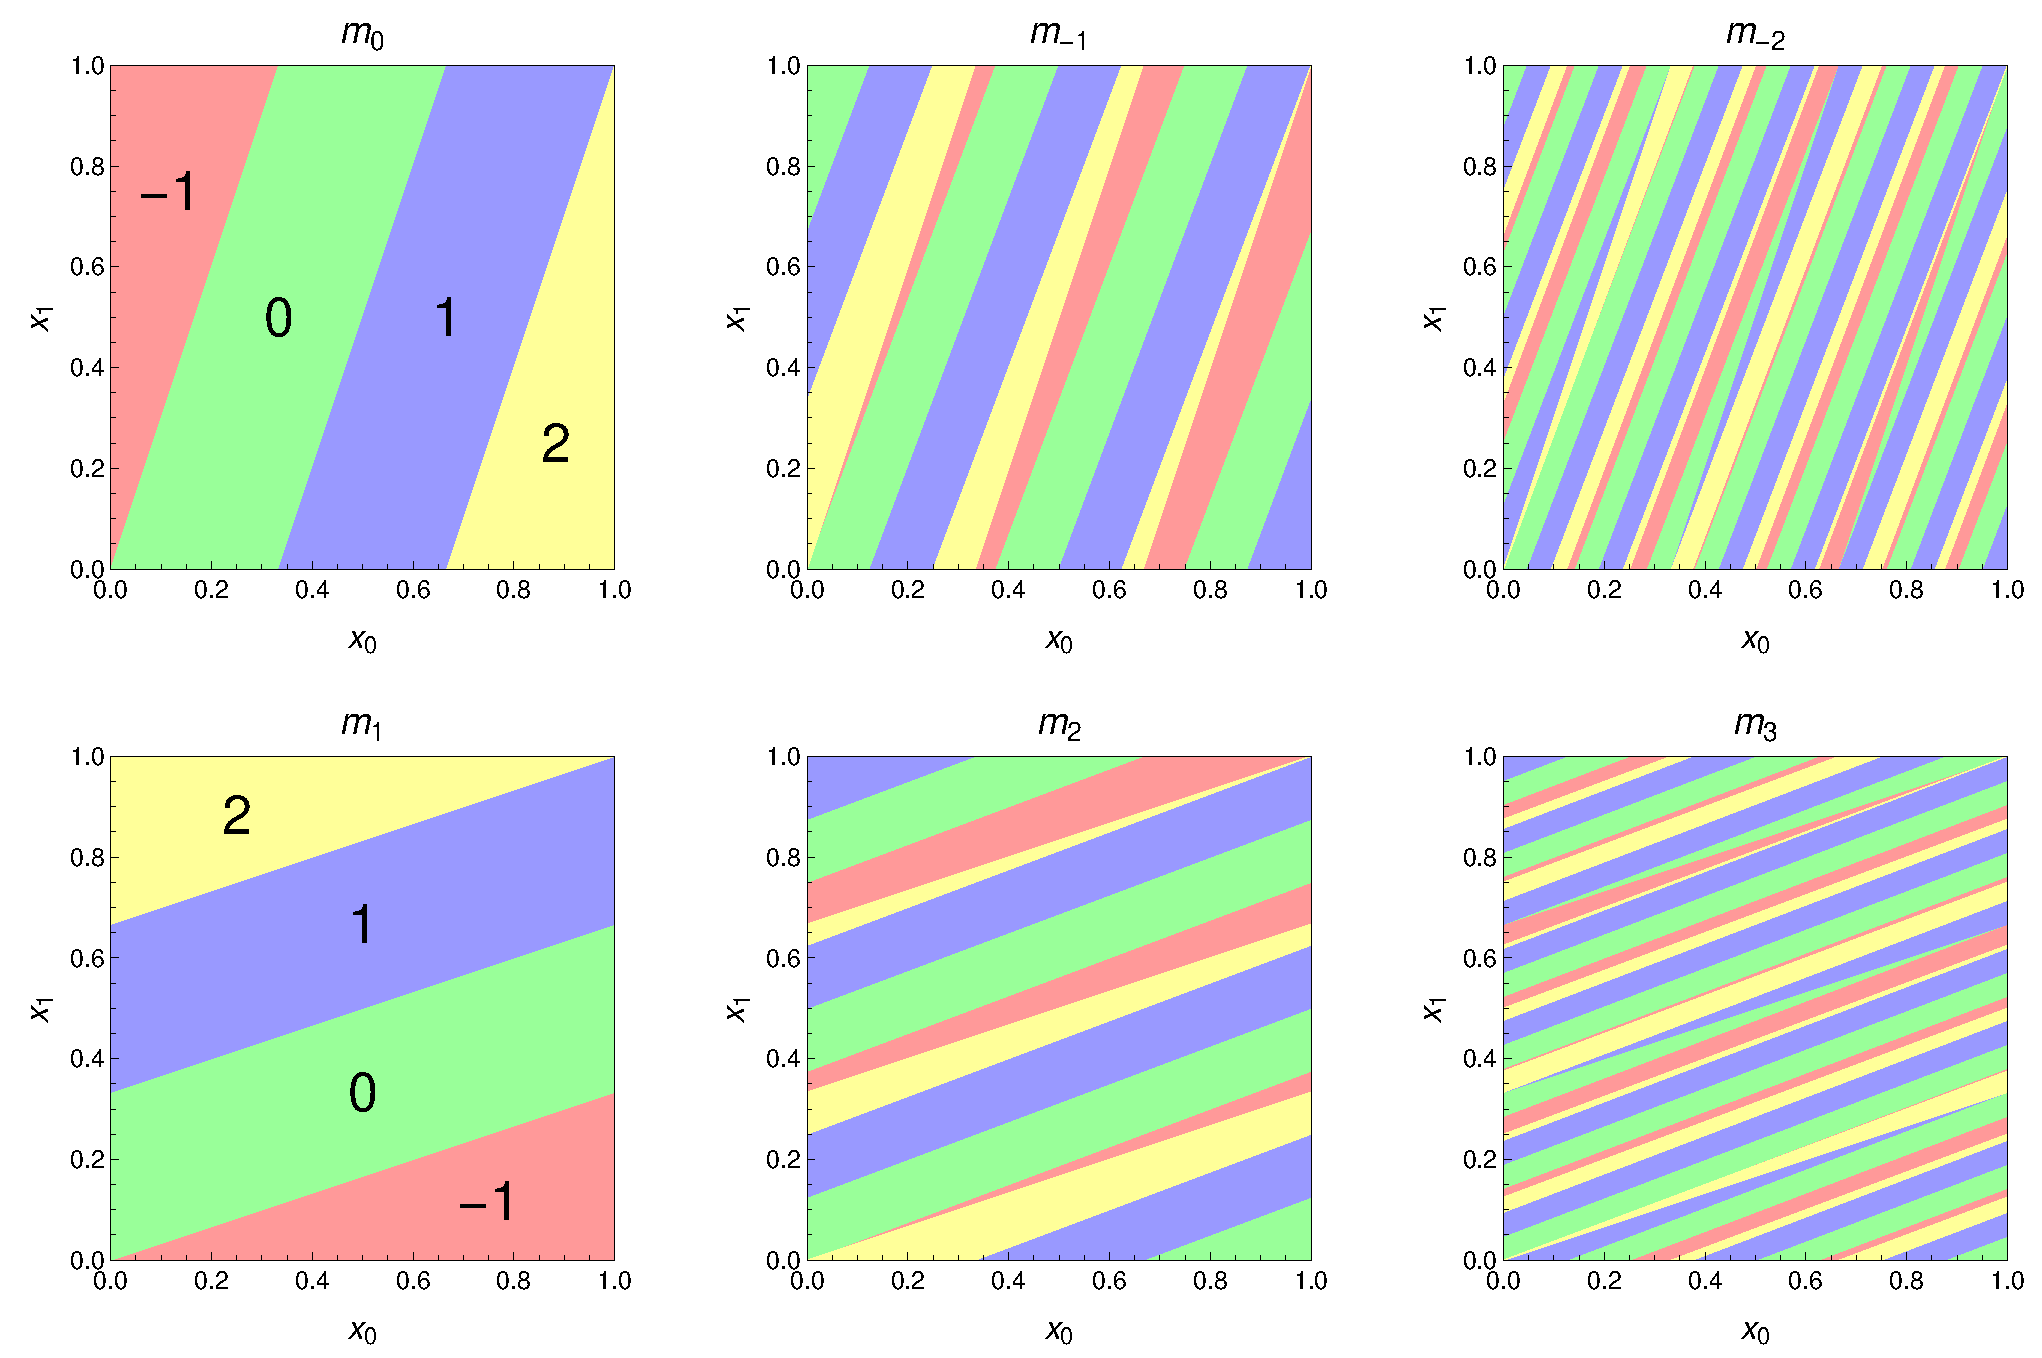
\includegraphics[width=0.95\textwidth]{SingleCat1Symbol}
	\caption{\label{fig:SingleCat1Symbol}
(Color online) $\ell = 1$ {\statesp s} on $(\ssp_{0},\ssp_{1})$  \statesp\ with respect
to symbols $\Ssym{t}$, $t = 0, -1, -2, 1, 2, 3$ for $s=3$. In each {\brick} values
of $\Ssym{t} = -1, 0, 1, 2$ are shaded with light red, green, blue, and yellow,
respectively, and each color has the same total area ($1/6$ for $\Ssym{t} = -1,
2$, $1/3$ for $\Ssym{t} = 0, 1$) in all {\brick s}. All boundary lines are straight
lines with rational slopes, while the slopes tend to irrational values set by
stable/unstable directions of the cat map exponentially fast in the limit $t
\rightarrow \pm\infty$.
	}
\end{figure}
%%%%%%%%%%%%%%%%%%%%%%%%%%%%%%%%%%%%%%%%%%%%%%%%%%%%%%%%%%%%%%%%%%

%%%%%%%%%%%%%%%%%%%%%%%%%%%%%%%%%%%%%%%%%%%%%%%%%%%%%%%%%%%%%%%%%%
\begin{figure}
	\centering
[the same plot as \reffig{fig:SingleCatPartit}]
	%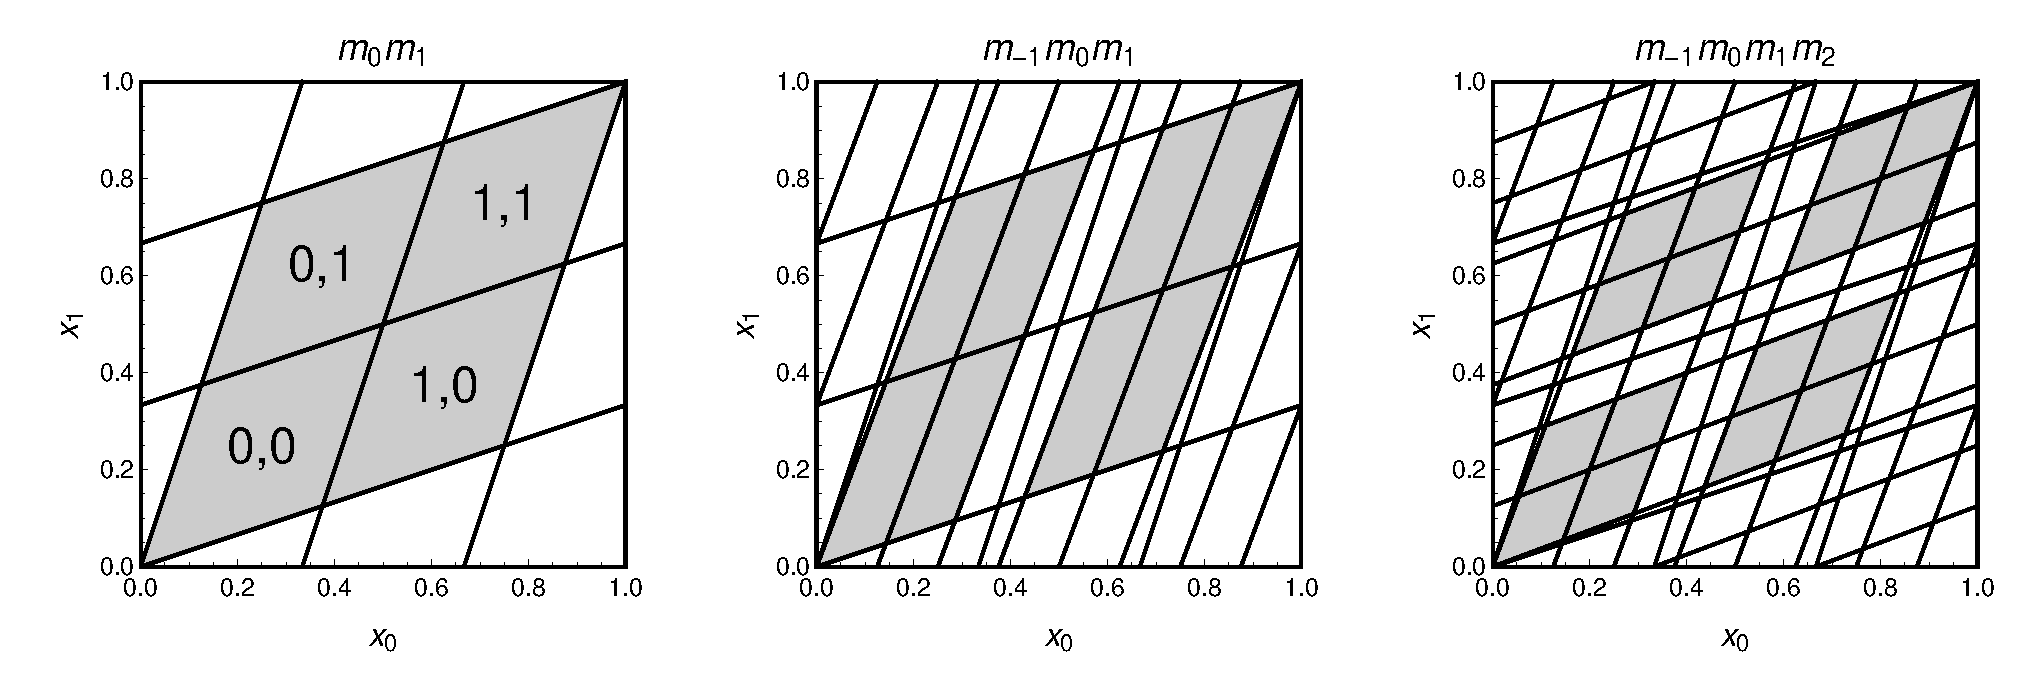
\includegraphics[width=0.95\textwidth]{SingleCatMultiSymbol}
	\caption{\label{fig:SingleCatMultiSymbol}
$\ell = 2, 3, 4$ {\statesp s} on $(\ssp_{0},\ssp_{1})$  \statesp\ for $s=3$, using {\brick s}
$\Ssym{0} \Ssym{1}$, $\Ssym{-1} \Ssym{0} \Ssym{1}$, and $\Ssym{-1} \Ssym{0} \Ssym{1} \Ssym{2}$ from the $\ell = 1$
diagrams. Shaded diamonds or rectangles correspond to sequences of all
interior symbols $(0, 1)^{\otimes \ell}$, having a total area of $4 \times
1/8$, $8 \times 1/21$, $16 \times 1/55$ respectively from left to right.
	}
\end{figure}
%%%%%%%%%%%%%%%%%%%%%%%%%%%%%%%%%%%%%%%%%%%%%%%%%%%%%%%%%%%%%%%%%%

Li Han text: ``
To generate such {\statesp} partitions, we start with length $\ell=1$. Consider
first the symbol $\Ssym{0} = s \ssp_0 - (\ssp_1 + \ssp_{-1}) =
\left\lfloor s \ssp_0 - \ssp_1 \right\rfloor$, where $\left\lfloor \cdots
\right\rfloor$ is the floor function. $\Ssym{0}$ has symbol boundaries
which are equally spaced parallel lines of slope $s$ and passing through
$(\ssp_0, \ssp_1) = (0, 0), (1, 1)$. We then look at the time-evolved
images of these symbol regions under forward map \refeq{eq:StateSpCatMap}.
The transformed region therefore means that at coordinate $(\ssp_{t+1},F
\ssp_{t+2})$ the point has symbol $\Ssym{t}$, which in turn implies that
when interpreted back to $(\ssp_{0},\ssp_{1})$  \statesp, a point is
associated with symbol $\Ssym{-1}$. As a result, we can generate all
length-1 {\statesp s} corresponding to symbols $\Ssym{t}$, $t = 0, \pm1,
\pm2, \cdots$ on the $(\ssp_{0},\ssp_{1})$  \statesp\ simply by applying
the forward map \refeq{eq:StateSpCatMap} or its inverse. We plot such
length-1 diagrams in \reffig{fig:SingleCatPartit} for symbols $\Ssym{0},
\Ssym{-1}, \Ssym{-2}$ (top), and $\Ssym{1}, \Ssym{2}, \Ssym{3}$ (bottom),
and call them different {\brick s}. Note that any of the {\brick s} can be used
to recover the 1-symbol measure $f_1(m)$ by calculating the total of
respective region areas, while with {\brick s} $\Ssym{0} = \left\lfloor s
\ssp_0 - \ssp_1 \right\rfloor$ and $\Ssym{1} = \left\lfloor s \ssp_1 -
\ssp_0 \right\rfloor$ the computations are the easiest, which have symbol
boundaries of slopes $s$ and $1/s$ respectively.

The fact that $\Msr(m
\in \Ai)$ are all equal and twice of $\Msr(m \in \Ae)$ is also obvious
from the $\Ssym{0}, \Ssym{1}$ {\brick s} of length-1 {\statesp s}.

A length-$\ell$ {\statesp} is then the superposition of any $\ell$
consecutive {\brick s} of length-1 diagrams, while a choice that is
symmetric about {\brick} $\Ssym{0}$ or $\Ssym{0}$ and $\Ssym{1}$ will
make the amount of calculations minimal. We have evaluated $\Msr(\m)$ up
to $\ell = 12$ from both \refeq{FreqDecomp} and symbolic diagrams for
$s=3$, $4$, $5$, and they are consistent. In \reffig{fig:SingleCatPartit}
we plot the symbolic diagrams for 2, 3, and 4 consecutive symbols using
{\brick s} $\Ssym{0,1}$, $\Ssym{-1,0,1}$, and $\Ssym{-1,0,1,2}$ of
\reffig{fig:SingleCatPartit}. Sequences of all interior symbols
correspond to congruent parallelogram regions whose opposite sides are
exactly parallel, and for even $\ell$ the regions are diamonds whose
sides are of equal length. Sequences of symbols from both \Ai\ and \Ae\
are not all admissible, which is the topic of next section. Here we note
that the corresponding regions of such sequences have general polygon
shapes and are not parallelograms, no matter which consecutive set of
{\brick s} we use.

%%%%%%%%%%%%%%%%%%%%%%%%%%%%%%%%%%%%%%%%%%%%%%%%%%%%%%%%%%%%%%%%%%%%%%%%
%    \PC{2016-12-27} {reuse this text from \reffig{fig:SingleCatPartit}? ``
All boundary lines are straight
lines with rational slopes, while the slopes tend to irrational values set by
stable/unstable directions of the cat map exponentially fast in the limit $t
\rightarrow \pm\infty$.
%    }
%%%%%%%%%%%%%%%%%%%%%%%%%%%%%%%%%%%%%%%%%%%%%%%%%%%%%%%%%%%%%%%%%%%%%%%%

From \refeq{FreqDecomp} the measure $\Msr(b)$ for a {\brick} $b =
\Ssym{1} \Ssym{2} \cdots \Ssym{\ell}$ is proportional to the area
of the polygon defined by inequalities (\ref{SquareCut1}).

The full list of measures $\Msr(\Ssym{1} \Ssym{2} \cdots \Ssym{\ell})$
has a tensor structure of tensor rank $\ell$ with each index running over
$\A$ and can be interpreted as a joint probability function.
''

Boris results.tex text: ``
whose lower left corner is the $(n,t)$ lattice site
\[
 \R_{nt} =\{(n+i, t+j) | i= 0, \dots, \ell_1-1, j= 0,\dots, \ell_2-2 \}
\,,
\]

It is straightforward to see that when \Mm\ is such that all symbols $\Ssym{z}$
belong to $\Ai=\{0,\dots,s-4\}$ then    \Mm\ is always admissible. By
positivity of  Green's function (see \refappe{sect:Green}) it follows
immediately that  $0 <\ssp_{z}$  while the condition
$\sum_{z'\in\integers}\gd_{zz'}=s-2$ implies that $\ssp_z\leq 1$.

''

Predrag text, recycle: ``
Here the piecewise linearity of the {\catlatt} enables us to go far analytically.
Essentially, as the cat map stretching is uniform, distinct admissible symbol
\brick s count all \brick s of a given shape (they all have the same
stability, and thus the same dynamical weight), and that can be accomplished
by linear, Green's function methods.
''

Predrag removed Boris poetry:
``
The  alphabet  separation into interior and external parts  nicely
illustrates  the  transition of the model from the correlated regime   to the
uncorrelated  Bernoulli process as parameter  $s$ in \refeq{LinearConn} tends
to $\infty$. Indeed, the number of external symbols in \Ae\ is fixed within a
given differential operator $\Box$  structure, while  the number of interior
symbols in \Ai\  grows linearly with the parameter $s$ controlling the
strength of chaos in a single map.   For {cat map} this transition can
be achieved by merely increasing the time step of time evolution. Increasing
the time step from $1$ to $2$ leaves the form of equation \refeq{OneCat}
intact, but renormalizes the  constant  $s\to s^2-1$.  This reflects the fact
that $\phi^2$  is more ``chaotic'' than  $\phi$. With an increase of  $k$
the map $\phi^k$ resembles more and more uncorrelated   Bernoulli process.
Similar transition can be observed  in the coupled  $\integers$ map lattices,
with a caveat that switch   from $\Phi$ to  $\Phi^k$ renormalizes  not only
the constant $s$, but   $\Box$  itself. The resulting equation of motion will
contain an  elliptic operator $\Box^{(k)}$ of higher order. Still,  it is
straightforward  to see that   the number of external symbols  is controlled
by  the order of the  operator $\Box^{(k)}$ which  grows linearly with $k$.
On the other hand, the number of interior symbols grows in the same way as
the constant  $s$ \ie, exponentially.
''

%%%%%%%%%%%%%%%%%%%%%%%%%%%%%%%%%%%%%%%%%%%%%%%%%%%%%%%%%%%%%%%%%%%%%%%%
%   \PC{2017-02-16} {
Replaced $N$ (for $N$ ``particles'') by $L$ (for spatial
extent) throughout
%    }
%%%%%%%%%%%%%%%%%%%%%%%%%%%%%%%%%%%%%%%%%%%%%%%%%%%%%%%%%%%%%%%%%%%%%%%%

\BGpost{2019-09-10}{
Old version, now replaced in results.tex by a more compact paragraph:

\medskip

To be specific, let \R\  be a   rectangular $[\ell_1\!\times\!\ell_2]$ region,
and let
\(
\Mm_{\R} % =\{\Ssym{z}\in \Mm | z\in \R \}
\)
be the  $[\ell_1\!\times\!\ell_2]$
\brick\ of \Mm\ symbols from
the alphabet $\A$.
Let
\(
\mathcal{N}(\Mm_{\R}|\Mm_{[L\!\times\!T]})
\)
be the number of times a given symbol {\brick} $\Mm_{\R}$ appears anywhere within
a much larger admissible symbol {\brick} $\Mm_{[L\!\times\!T]}$
cut out from a {\spt}ly infinite generic solution \Mm\ of the
\catlatt\ \refeq{LinearConn}.
The $d=1$ cat map is known to be fully hyperbolic and ergodic for $s>2$, with a
unique invariant natural measure $\Msr$  in the \statesp\
\refeq{eq:CatMapIntr} of the system.
The $d=2$  \catlatt\  is fully hyperbolic and ergodic for
$s>4$, see \refeq{qudreq}. In the language of spatially extended systems, we
assume that a steady state {\spt}ly chaotic solution is on average
{\spt}ly invariant, so the number of times a \emph{given} admissible
\brick\ $\Mm_{\R}$ shows up over a region $[L\!\times\!T]$ is expected to grow
linearly with the area $LT$. Hence a \emph{relative} frequency of the
occurrence of  the {\brick} $\Mm_{\R}$ can be defined as
\beq
f(\Mm_{\R}|\Mm_{[L\!\times\!T]})
    =
\frac{1}{LT}
\mathcal{N}(\Mm_{\R}|\Mm_{[L\!\times\!T]})
\,.
\ee{relFreqR}
With $L$ and $T$ increasing at comparable rates (for example,
take a square $[L\!\times\!T]$, with $L=T$), the ergodic measure of finding the
{\brick} $\Mm_{\R}$ across the infinite {\spt} domain is given by
\beq
\Msr(\Mm_{\R}) =
\lim_{L,T \to\infty}
f(\Mm_{\R}|\Mm_{[L\!\times\!T]})
\,,\qquad
\sum_{{\Mm_{\R}}} \Msr({\Mm_{\R}}) =1
\,.
\ee{relFreq}

\bigskip

For an ergodic system with a  unique invariant natural measure $\Msr$, the
limiting frequencies  $f(\Mm_{\R})$ are equal to the measures $\Msr( \pS_{\R})$
of the cylinder sets $ \pS_{\R}$, defined as sets of \statesp\ points $\Xx_{\R}$
having $\Mm_{\R}$ symbolic representation over the region \R. For this reason, we
sometimes refer, with a slight abuse of notation, to the frequencies
$f(\Mm_{\R})$ defined by \refeq{relFreqR} as measures of $\Mm_{\R}$ in the limit
$L,T \to\infty$, and denote them by $\Msr(\Mm_{\R})$ in what follows.
    }

\item[2016-11-20 Boris]
The {\spt} symbols follow from the Newtonian equations
in $d$ {\spt} dimensions
\bea
\Ssym{n,j} &=& (q_{n,j+1} -2 q_{n,j} + q_{n,j-1})
         + (q_{n+1,j}  -2 q_{n,j} + q_{n-1, j}) -  (s-4) q_{n,j}
        \continue
{\m} &=& [\Box + 2d\mathsf{1} -s\mathsf{1}]\, {\q}
\,.
\label{PC}
\eea

%As our ultimate goal is semiclassical quantization of a quantum many-particle
%system (or a quantum field theory),

%\PCpost{2017-01-03} {
%I changed the sign of $\Ssym{nt}$ in \refeq{CoupledCats},
%as in \refeq{LinearConn}, do all cats approve?
%    }
%\BGpost{2017-07-31}
%{Changed it back. Our present convention is the opposite one!}

    \PCpost{2017-02-16} {
To me, the Green's functions look strictly positive. Must harmonize
definitions \refeq{GreenFun0}, \refeq{GreenFun00}, \refeq{GreenFun000},
\refeq{LinearConn} and
\refeq{OneCat}, originating in Boris' flip-flop $\Ssym{t}\to-\Ssym{t}$

Is there a reference to Green's functions in terms of Chebyshevs?
    }
\BGpost{2017-08-02} {Yes,  and  it is OK with our present convention  -
Green's functions must be positive.}
    \BGpost{2017-08-02}{
%    I have checked the consistency of the symbol definitions ($m\to -m$
%    issue). Double check  might be needed in captions, but otherwise OK.
    Rule-of-thumb - internal symbols are non-negative, Green's functions
    are positive.}

\BGpost{2017-07-31}{
``As every Anosov automorphism is topologically conjugate to a linear cat
map ...'' Is it really true ?
}

    \PCpost{2017-08-11} {
That's what I read in some of the articles cited. But no need to say it
here, so now this is removed from our article.
    }

    \PCpost{2016-11-13}{ to all cats -
where we write \refeq{OneCat},
Percival and Vivaldi\rf{PerViv} write their Eq.~(3.6)
\(
(\Box +2 - s) \ssp_{t} = -b_t
\) %ee{PerViv3.6Bl}
so their ``stabilising impulses'' $b_t$  have the opposite sign to our
``winding numbers'' $\Ssym{t}$ (defined on $\ssp\in[0,1)$).\\
To all cats: keep checking that  after your flip of signs of $\Ssym{t}$'s
Eqs.~\refeq{LinearConn}, \refeq{OneCat}, \refeq{Coord} and \refeq{PC} are
consistent.
    }
\BGpost{2017-07-31}
{ Changed time ago. They should have the same sign as Percival and
Vivaldi i.e., our  $m$ are positive!}

%    \PCpost{2017-08-05}{dropped this: ``
%We illustrate this by first reviewing the $d=1$ case
%(introduced in \refref{PerViv}), but the focus of the paper is the $d=2$
%case (introduced in \refref{GutOsi15}).
%    ''}

%%%%%%%%%%%%%%%%%%%%%%%%%%%%%%%%%%%%%%%%%%%%%%%%%%%%%%%%%%%%%%%%%%%%%%%%%
%    \PCpost{2016-12-15} {
%%Definition \refeq{relFreq} is not normalized correctly.
%I worry a
%bit as whether it makes sense. It works for a single letter, $\R =
%[1\times 1]$. Have to argue that for larger \brick s
%\(
%   \mathcal{N}(\Mm_{\R}|\Mm_{[L\!\times\!T]})
%\)
%does not grow exponentially or
%as a power of $LT$? Perhaps obvious...
%    }
%    \BGpost{2017-07-29}{
%Looks like a misunderstanding here. I have tried to make the text more
%clear. We should distinguish between  frequencies in \refeq{LinearConn}
%and measures $\Msr(\Mm_{\R})$, at least on the level of definitions. They
%coincide for systems with unique ergodic measure.
%%and it is our assumption through the whole paper that this is the
%%case.(But we lack a mathematical prove of this. )
%For me  the normalization looks
%correct. Note that  $LT$ is  just the  total number of patterns within
%$\Mm_{[L\!\times\!T]}$ (minus boundary ``effects``).
%    }
%%%%%%%%%%%%%%%%%%%%%%%%%%%%%%%%%%%%%%%%%%%%%%%%%%%%%%%%%%%%%%%%%%%%%%%
   \PCpost{2017-08-11} {
I now get it. $LT$ is the area of \R. The  total number of \brick s
grows exponentially with the size of $\R$ and
is bounded from above by $(LT)^{|\A|}$.
You are saying that the number of
times a \emph{single} admissible \brick\ $\Mm_{\R}$ shows up over a region
$[L\!\times\!T]$ grows linearly with the area $LT$, and so does the
sum over frequencies of all distinct admissible \brick s ${\Mm_{\R}^{'}}$?
These ``frequencies'' are \emph{relative}, in the sense that correct
normalization is not \refeq{relFreq}, but
\beq
\Msr(\Mm_{\R}) = \frac{f(\Mm_{\R})}{
\sum_{{\Mm_{\R}^{'}}} f(\Mm_{\R}^{'})
            }
\,.
\ee{freqNormalized1}
    }
%%%%%%%%%%%%%%%%%%%%%%%%%%%%%%%%%%%%%%%%%%%%%%%%%%%%%%%%%%%%%%%%%%%%%%


    \PCpost{2017-08-05 }
    {Cylinder sets are subtle: if we were counting only {\em admissible}
$\Xx$, the cylinder set would be much smaller. But we almost never know
all inadmissible states.
\index{block!finite sequence}
\index{cylinder!set}
    }

 \BGpost{2017-07-31}
 {Li subsection {\em {\Brick s} of length $\ell$,}
% \label{sect:catGenerL}
 was siminos/cats/catGenerL.tex 2017-02-17, mostly
 contained repetitions of the previous stuff. Did not think we needed it. Few
 usable things  could be brought to other places. Agree?}
 \PCpost{2017-08-23}{Done.}

 \PCpost{2017-08-26}{Removed: ``
                                                \toCB
The term $\Box + 2 d\,\mathsf{1}$ is the standard statistical mechanics
diffusive inverse propagator that counts paths on a $d$\dmn\
lattice\rf{CBook:appendSymm}, and $-s\mathsf{1}$ is the on-site cat map
dynamics
(for the Hamiltonian formulation, see \refappe{sect:HamiltonCatLatt}).
        }

\BGpost{2017-08-05} {
Something unclear here (at least for me). ``The iteration of a map
$g(\ssp_{t})$ generates a group of  \emph{time translations}''.  Why
translations?   $g$ is a (time) map  acting  on all sites of lattice
independently (no interaction). Note: I think the models in \rf{PesSin88} and
\rf{BunSin88} are of the  same type. Both  can be thought of as products of
two maps: `` Interactions'' $\cdot$ ``Single particle propagations'' (i.e.,
product of $g$'s)
\\
{\bf 2017-09-04 Predrag}: You are right, I have rewritten that text now.
  }

    \PCpost{2017-08-28} {
For the Dirichlet (as opposed to periodic) boundary condition, which breaks
the translational symmetry, we take the very unphysical b.c. $\ssp_z=0$ for
$z\in\R$. Finite windows into turbulence that we describe by our symbol
\brick s never have such edges. Methinks...
    }
%%%%%%%%%%%%%%%%%%%%%%%%%%%%%%%%%%%%%%%%%%%%%%%%%%%%%%%%%%%%%%%%%%%%%%%%

\BGpost{2017-09-12}{
This equation
\bea
\ssp_{n, t+1}&=&p_{nt}+(s-3)\ssp_{nt} - (\ssp_{n+1,t} - 2\ssp_{nt} + \ssp_{n-1,t}) - {m}^\ssp_{n,t+1}
\continue
p_{n,t+1}&=&p_{nt} + (s-4) \ssp_{nt} - (\ssp_{n+1,t} - 2\ssp_{nt} + \ssp_{n-1,t}) - {m}^p_{n,t+1}
\,.
\label{eqmotion0}
\eea
seems wrong. We use \refeq{eqmotion}.
    }

    \BGpost{2017-09-14} {
Recall that (the Dirichlet) $\gd_{zz''}$ is a function of both $z$ and $z''$
and not just of the  distance between them $|z-z''|$.
    }

    \PCpost{2017-09-04}{
``integer $s>4$'' is not the correct condition, for $d=2$ $s=4$ is presumably
already hyperbolic. To add to the confusion, in his report Adrien computes
for $s=3$, the case with no interior alphabet symbols. So $s>2$ is the
correct hyperbolicity condition for all $d$?
Give the correct condition on $s$, explain it.
    }

\BGpost{2017-09-12}{
Here are the  answers to  this and co. questions over the paper.
\begin{enumerate}
  \item
The system is uniformly (fully) hyperbolic for  $s>2d$. This means all
eigenvalues of linearized map  (see  \refeq{qudreq}  for $d=2$) are  either
$|\ExpaEig|<1$  (stable subspaces)  or $|\ExpaEig|>1$ (unstable subspaces).
  \item
For $s=2d$ the system is partially hyperbolic. This means everything as above
except two  Lyapunovs for  which   $\ExpaEig=1$ (neutral subspaces).
  \item
For $|s|<2d$  system is non-hyperbolic. Apparently for everything in this
paper 1 $\&$ 2 is OK. But
  \item
drastically changes everything (suspect  a phase transition in physics jargon
i.e., non-unique SRB measure). So whatever we consider  in the paper should
be for $s\geq 2d$.
\end{enumerate}
    }

 \BGpost{2017-09-14} {
A comment on $s=2d$ case (do not know how much of it we need for the paper).
Our results in this paper require in principle  $s>2d$ (all Lyapunovs are
positive). However certain things still work (by whatever reason)  for $s=2d$
as two figs in \refsect{sect:catLattEntropy} show. In this case the total
momentum $\sum_{n=1}^L p_{nt}$ is preserved. This can be seen from the
invariance of \refeq{LinearConn} under   translation  $x_{nt}\to
x_{nt}+\alpha$. So the system is not ergodic  and linear encoding is not one
to one (different trajectories might have the same symbolic representation).
However, it is (probably)  ergodic on the shell   $\sum_{n=1}^L p_{nt}=const.$
This is probably the reason why  our formulas for frequencies of  $\Mm_{\R}$
still work.
 }

\BGpost{2017-09-26}{Dropped this:
``
with the corresponding probability of occurrence of a fixed symbol
{\brick} $\Mm_{\R}$ given by
\[
\Msr(\Mm_{\R}|\Mm_{[L\!\times\!T]}) =
\frac{f(\Mm_{\R}|\Mm_{[L\!\times\!T]})}
     {
\sum_{{\Mm_{\R}^{'}}} f(\Mm_{\R}^{'}|\Mm_{[L\!\times\!T]})
     }
\,,\qquad
\sum_{{\Mm_{\R}}} \Msr({\Mm_{\R}}|\Mm_{[L\!\times\!T]}) =1
\,,
\]  %\ee{freq2measure}
where the sum goes over all distinct admissible {\brick s}
${\Mm_{\R}^{'}}$.''

The point is that
\[
\sum_{{\Mm_{\R}}}\mathcal{N}(\Mm_{\R}|\Mm_{[L\!\times\!T]})= LT - \mbox{
``Terms linear in L and T''}.
\]
So no need in an artificial normalization -
normalization in  \refeq{relFreq} would follow anyhow.
}

 \BGpost{2017-09-14} {Replaced this eq.
\beq
\Mm\cup\partial\R
    =
\left[\begin{array}{c}
\ssp_{12}   \\
\ssp_{01}~\Ssym{11}~\ssp_{21} \\
\ssp_{10}   \\
\end{array}\right]
    =
\left[\begin{array}{c}
\ssp_{2}   \\
\ssp_{1}~\Ssym{11}~\ssp_{3} \\
\ssp_{4}   \\
\end{array}\right]
\ee{block1x1border}
by the first plot in \reffig{fig:block2x2}.
 }

    \PCpost{2016-11-15, 2017-08-28} {
Note: When I look
at the intersection of the diagonal with the partition strips in by
inspecting \reffig{fig:SingleCatPartit}, I find that the Fibonacci
numbers 1,2,3,5, ... give the numbers of periodic points, in agreement with
the \AW\ Markov partition. So the linear
code is not a generating partition, but \po s do the right thing anyway.
    }

\PCpost{2018-04-05 to Adrien from}{
I think \reffig{fig:AKScloseActSp} is really hard to explain to a reader;
why these axes, how did all points get mapped into the same unit square,
why there are huge empty swaths - all stuff that distracts from the
main point which is that $x_z$'s within the center of the shared symbol \brick\
are exponentially close.
    }

\PCpost{2018-04-05}{
I think we can simplify this greatly, using the fact that the (damped)
{\sPe} \refeq{LinearCatLatt} is linear, so one can subtract
patterns in order to visualize their distance.

In order to have a 2\dmn\ visualization for each \brick,
color the symbol $\Mm_j$ $[\speriod{1}\!\times\!\speriod{2}]$ \brick\ with discrete
color alphabet \Ai, as in \reffig{fig:AKScloseActSymb},
and the corresponding state $\Xx_j$ $[\speriod{1}\!\times\!\speriod{2}]$ \brick\
with colors chosen from a continuum color strip.

As this is a linear problem, you can also represent closeness of two
$[\speriod{1}\!\times\!\speriod{2}]$ \brick s by using this coloring scheme for
$\Mm_2-\Mm_1$ and $\Xx_2-\Xx_1$.
%To find the closest ``distance'' between
%2-tori, you will have to go through all cyclic permutations of the second one
%to align it optimally
%(or, if you understand ChaosBook course, you'll have to `slice').

For pairs of distinct 2-tori which share the same region of $\Ssym{z}$'s, or a
single 2-torus in which the same region of $\Ssym{z}$'s appears twice, the
states $\ssp_z$ in the center of the region should be exponentially close,
in order to demonstrate that they shadow each other.

So, replace \reffig{fig:AKScloseActSp} by
(a) $\Mm_2-\Mm_1$ from \reffig{fig:AKScloseActSymb} (it will be all the same
    color in the shared region), and
(b) plot $\Xx_2-\Xx_1$. Mark the lattice point $z$ with the minimal value of
    $|x^{(2)}_z-x^{(1)}_z|$ on this graph, and in the text state the minimal value of
    $|x^{(2)}_z-x^{(1)}_z|$.
    You can also state the mean Euclidean (or L2) distance between the
    two \twots:
\beq
d_{\Xx_2-\Xx_1} =
         \left(\frac{1}{LT} \sum_z (x^{(2)}_z-x^{(1)}_z)^2\right)^{1/2}
\,,
\ee{twotsDist}
or distance averaged over the lattice points restricted a region \R.
\\ \textcolor{blue}{(taken care of by AKS)}
    }

\AKSpost{2018-04-13}{
After reconstructing the orbits separately, I plotted the distance
between the positions in $(q,p)$ space for each lattice site $z$, see
the new \reffig{fig:AKSs7dist}, meant to replace the current
\reffig{fig:AKScloseActSp}.
\color{red}{Still have to use sensible color ranges,
and compute} \reffig{fig:AKSs7dist}\,(b).
%%%%%%%%%%%%%%%%%%%%%%%%%%%%%%%%%%%%%%%%%%%%%%%%%%%%%%%%%%%%%%%%%%%%%%%
\begin{figure}
\begin{center}
(a) 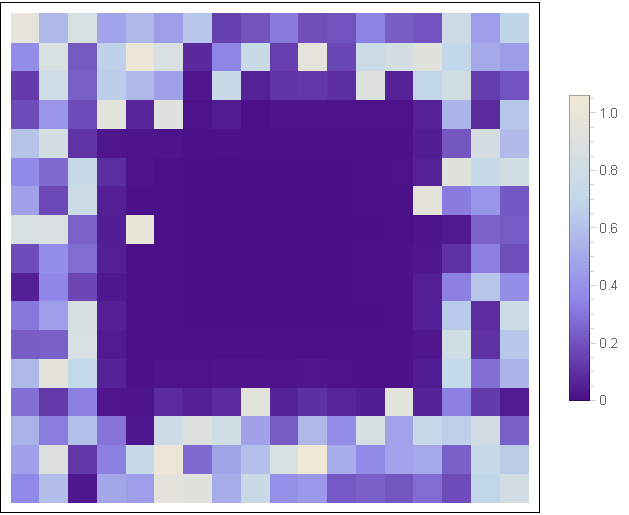
\includegraphics[width=0.45\textwidth]
{AKSs7distM1M2} %\hspace{0.7cm}
(b) 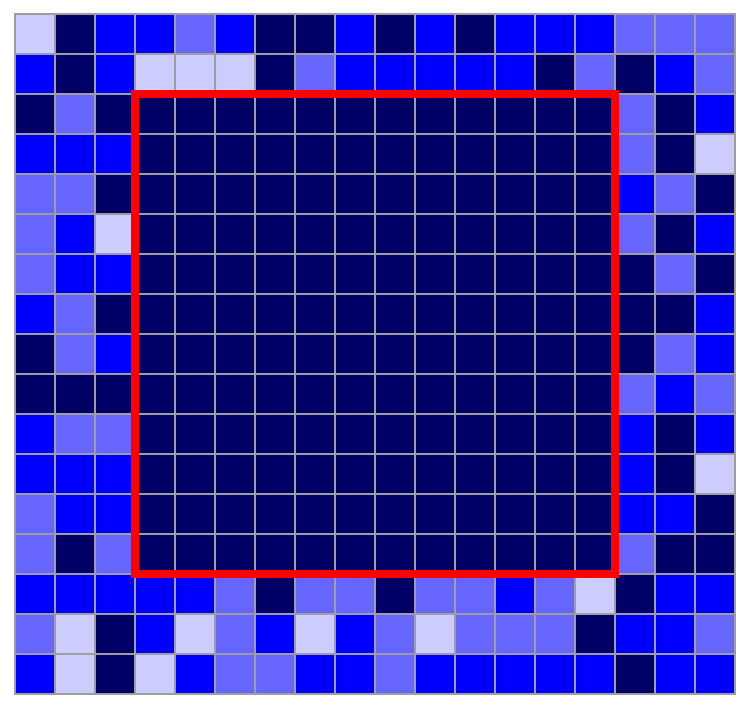
\includegraphics[width=0.37\textwidth]
{AKSs7distM1M2log}
\end{center}
\caption[]{
(Color online)
    (a)
\(\Xx_{2,z}-\Xx_{1,z}\,,\)
the site-wise distance between the \twots\ fields corresponding to the
two $[18 \times 18]$ \brick s
$\Mm_{1}$, $\Mm_{2}$ (colored tiles) of
\reffig{fig:AKScloseActSymb}\,(a,b).
    (b)
The plot of the site-wise symbol difference
\(
|\Mm_{2,z}-\Mm_{1,z}|
\)
 of  \reffig{fig:AKScloseActSymb}\,(b) and (b)
(for a better visualization, see \reffig{fig:AKSs7distupdated}).
}
\label{fig:AKSs7dist}
\end{figure}
%%%%%%%%%%%%%%%%%%%%%%%%%%%%%%%%%%%%%%%%%%%%%%%%%%%%%%%%%%%%%%%%%%%%%%%
\\ \textcolor{blue}{(taken care of by AKS)}
}

\PCpost{2018-04-13 to Adrien from}{
Also of interest might be the color-coded plot of value of $x_{q,p}$ for at
least one of them. Would be nice to check -at least once- whether there is
any relation to the corresponding  $m_{q,p}$ (probably there is no relation).

We'll have to rethink coloring (should be the same as  $m_{q,p}$, more or less).

As the distance decreases exponentially towards the center, you probably want
a color plot of
    $\ln |\ssp_{q,p}^{(2)} - \ssp_{q,p}^{(1)}|$
to resolve the small distances towards the center of the square.
\\ \textcolor{blue}{(taken care of by AKS)}
    }

%%%%%%%%%%%%%%%%%%%%%%%%%%%%%%%%%%%%%%%%%%%%%%%%%%%%%%%%%%%%%%%%%%%%%%%
\begin{figure}
\begin{center}
(a) 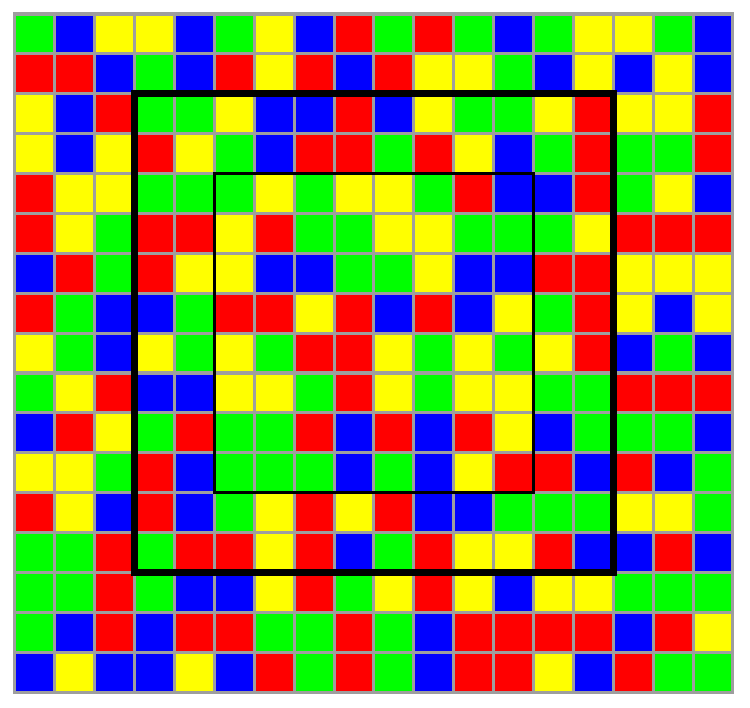
\includegraphics[width=0.45\textwidth]
{AKSs7colrBorderM1} %{AKSs7BlockBorderM1} %\hspace{0.7cm}
(b) 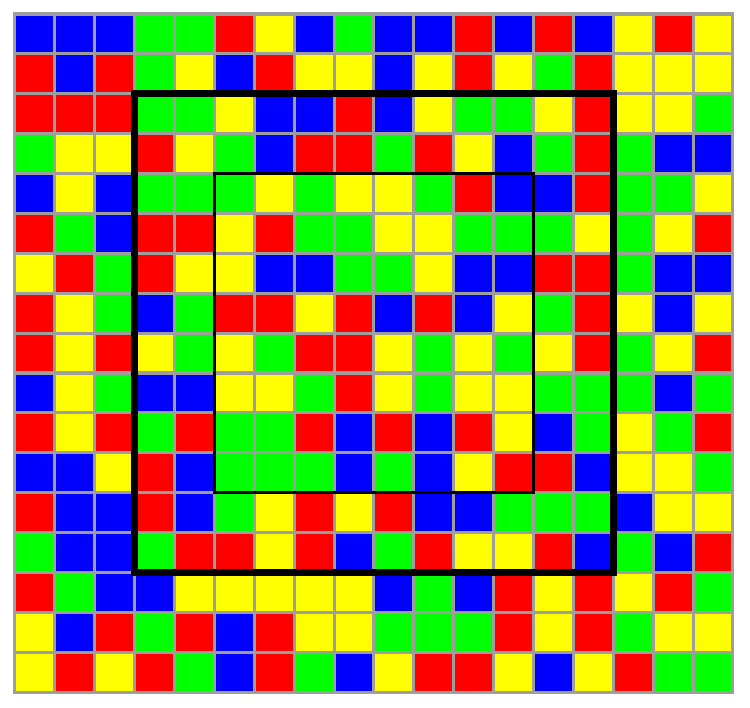
\includegraphics[width=0.45\textwidth]
{AKSs7colrBorderM2} %{AKSs7BlockBorderM2}
\end{center}
\caption[]{\label{fig:AKScloseActSymb}
\PCedit{Figure nixed by Boris 2019-08-21, replaced by digits
\reffig{fig:BGcloseActSymb}.}
%(Color online)
Symbolic representation (colored tiles) of two
$[L\!\times\!T] = [18 \times 18]$
{\twot} solutions of
\refeq{CoupledCats},
$s=7$,
that shadow each other within the shared
\brick\ $\Mm_{\R}=\Mm_{\R_{0}} \cup \Mm_{\R_{1}}$ (blue).
The symbols within \R, drawn randomly from the interior alphabet \Ai, are
the same for both solutions;
the symbols outside \R, also drawn randomly from \Ai, differ.
The shared \brick\ $\R=\R_{0} \cup \R_{1}$ is split into the interior region
$\R_{0}$ (bold blue) and the border strip $\R_{1}$ (blue).
%  AKS 2019-09-10
% (a) and(b) are in fact the color code \brick s a smaller size system than
% the one we use now in the main TEXT.
    }
\end{figure}
%%%%%%%%%%%%%%%%%%%%%%%%%%%%%%%%%%%%%%%%%%%%%%%%%%%%%%%%%%%%%%%%%%%%%%%

% \BGpost{2019-08-21} { % 2019-08-26 PC
%I prefer digits \reffig{fig:BGcloseActSymb}  rather than color
%\reffig{fig:AKScloseActSymb} for two reasons. Minor issue - colors are
%visible only online, slightly  more serious issue - colors will require a
%color map (to connect them with the code) = additional intermediate
%level. It also makes things more homogeneous = helps to understand
%\reffig{fig:AKSs13TwoBlock1} etc.
%\\ {\bf  implemented PC}
%\\ \textcolor{blue}{(taken care of by AKS)}
%    }

\BGpost{2017-08-02}
    {The representation \reffig{fig:BGcloseActSymb} has changed from
    digits to colors \reffig{fig:AKScloseActSymb}
    ({\bf PC} 2019-08-26 reverted this figure to digits).
    \\
    Was it try and see, or is it going to stay? In my
    opinion it is more colorful, but less informative. The reason is a)
    digits are directly $m_{nt}$ - no need to translate colors into
    numbers + make sense without  colors (on line). b) the encounters
    (regions with the same coding)   can be visualized   by coloring.}
    \PC{2017-08-11}
    {Well, that's a bit subjective - it is unintelligible to a human eye
    either way. I would keep this one figure as an illustration that
    color coding is an alternative to number coding.
    \\ \textcolor{blue}{(taken care of by AKS)}
}


 \BGpost{2019-08-21} { % 2019-08-26 PC
Now that we got rid of the color \reffig{fig:AKScloseActSp}, there's no
point in having two different colors in \reffig{fig:BGcloseActSymb} for
the overlapping regions of symbols, light blue for the outer region
called $\R_{1}$  in the paper, dark blue for the inner one called
$\R_{0}$.
\\ {\bf toDo}
\\ \textcolor{blue}{(taken care of by AKS)}
    }

 \BGpost{2019-08-21} {	
I like including the differences plot \reffig{fig:AKSs7dist}
or \reffig{fig:AKSLPS12}
(we have something similar in Our Paper\rf{GutOsi15} with Vladimir
Osipov)
{\bf (implemented PC 2019-08-27)}.\\
It should be included as addition to \reffig{fig:BGcloseActSymb}, and not
as substitution to it (it substitutes \reffig{fig:AKScloseActSp}, now
removed from the paper). Without \reffig{fig:BGcloseActSymb} it would be
difficult to digest and explain its content.}

\AKSpost{2019-10-30}{
I think by now we agreed we would keep the digits figure only. The
figures of symbolic difference (\reffig{fig:AKSs7dist}) and of symbolic
coloring (\reffig{fig:AKScloseActSymb}) are either outdated or ugly. We
can toss them out of the blog. \reffig{fig:AKSsymbol} and
\reffig{fig:AKScloseActSp} could be moved to another appendix. We could
also move \reffig{fig:AKSs7distupdated} to another appendix, as it is the
most recent ``difference of symbols" figure.\\
\textcolor{blue}{(taken care of by AKS)}
    }

 \PCpost{2019-08-27} {
If you mean ``metric distances'' of \GO\ figures A3 and C2, that is quite
different than our log(distance) plots. Problem is that \GO\ measure
Eucliden distance between symplectic phase-space points, not a meaningful
distance. Would have to subtract actions, but this is not a thing for
this paper...
    }

\AKSpost{2019-08-21} {
You mean \reffig{fig:AKSs7dist} here in \texttt{GHJSC16blog.tex}, \ie,
\reffig{fig:AKSLPS12}\,(a) which is the log of the norm of the
difference of the two trajectories in \statesp? I agree that if
anything, \reffig{fig:AKSLPS12}\,(a) should substitute
\reffig{fig:AKScloseActSp} and not \reffig{fig:BGcloseActSymb}.
What do you think on the updated color pattern,
\reffig{fig:AKSLPS12}\,(b)?
\\ \textcolor{blue}{(taken care of by AKS)}
    }

%\PCpost{2019-08-21} {
%Moved \reffig{fig:AKScloseActSp} from the  paper to here, replaced
%it by \reffig{fig:AKSLPS12}.
%                    }

 \BGpost{2019-08-26} {
Still not good enough. The coloring is too jumpy.   It should range from
white or light blue to dark blue. For a  more reasonable coloring  of
this type see figure~14 from Our Paper\rf{GutOsi15} \arXiv{1503.02676}.
Maybe also the periods of tori L, T  should be larger to make things
smoother.
%\\ {\bf toDo}
\\ \textcolor{blue}{(taken care of by AKS)}
        }

 \AKSpost{2019-08-21} {
 We still need the two symbolic representation figures in
\reffig{fig:BGcloseActSymb}.
In \reffig{fig:AKSsymbol} I have regenerated those symbolic
representation as numbers instead of colors, as an alternative to
\reffig{fig:BGcloseActSymb}. Which one do you prefer?
%\\ {\bf toDo}
\\ \textcolor{blue}{(taken care of by AKS)}
        }

 \BGpost{2019-08-21} {	
For \reffig{fig:RJsymbol} - a different coloring pattern is indeed needed
+ the size of the figures (a), (b) should be the same.
\\
{\bf AKS}
I agree. Except for the size, which should be the same as the current
\reffig{fig:BGcloseActSymb}\,(a).
\\ {\bf toDo}
\\ \textcolor{blue}{(taken care of by AKS)}
    }

%%%%%%%%%%%%%%%%%%%%%%%%%%%%%%%%%%%%%%%%%%%%%%%%%%%%%%%%%%%%%%%%%%%%%%%
\begin{figure}
\begin{center}
(a) 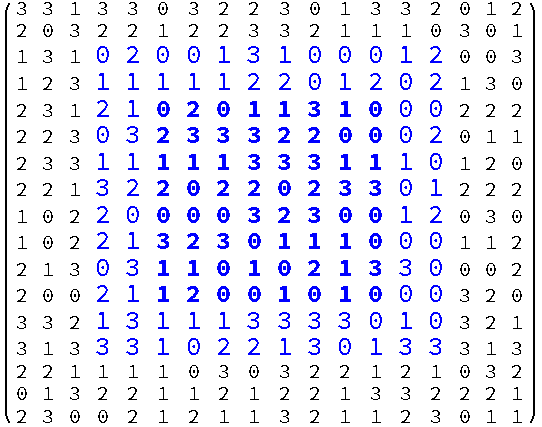
\includegraphics[width=0.45\textwidth]{AKSsymbol1}
%{AKSs7BlockBorderM1} %\hspace{0.7cm} %color: {AKSs7colrBorderM1}
(b) 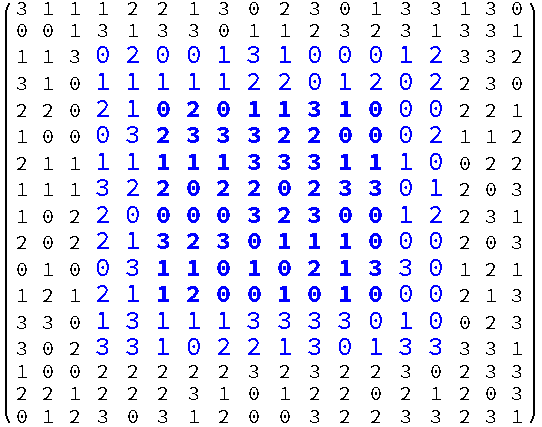
\includegraphics[width=0.45\textwidth]{AKSsymbol2}
%{AKSs7BlockBorderM2}                 %color: {AKSs7colrBorderM2}
\end{center}
\caption[]{
(Color online)
Symbolic representation (numbered tiles) of two
$[L\!\times\!T] = [18 \times 18]$
{\twot} solutions of
\refeq{CoupledCats},
$s=7$,
that shadow each other within the shared
\brick\ $\Mm_{\R}=\Mm_{\R_{0}} \cup \Mm_{\R_{1}}$ (blue).
The symbols within \R, drawn randomly from the interior alphabet \Ai, are
the same for both solutions;
the symbols outside \R, also drawn randomly from \Ai, differ.
The shared \brick\ $\R=\R_{0} \cup \R_{1}$ is split into the interior region
$\R_{0}$ (bold blue) and the border strip $\R_{1}$ (blue).
}
% in GHJSC16.tex: {fig:BGcloseActSymb}  %in blog, color: {fig:AKScloseActSymb}
\label{fig:AKSsymbol}  %in blog, color: {fig:AKScloseActSymb}
\end{figure}
%%%%%%%%%%%%%%%%%%%%%%%%%%%%%%%%%%%%%%%%%%%%%%%%%%%%%%%%%%%%%%%%%%%%%%%

%%%%%%%%%%%%%%%%%%%%%%%%%%%%%%%%%%%%%%%%%%%%%%%%%%%%%%%%%%%%%%%%%%%%%%%
\begin{figure} % PC 2019-08-27 replaced by \reffig{fig:AKSLPS12}
\begin{center}
(a) 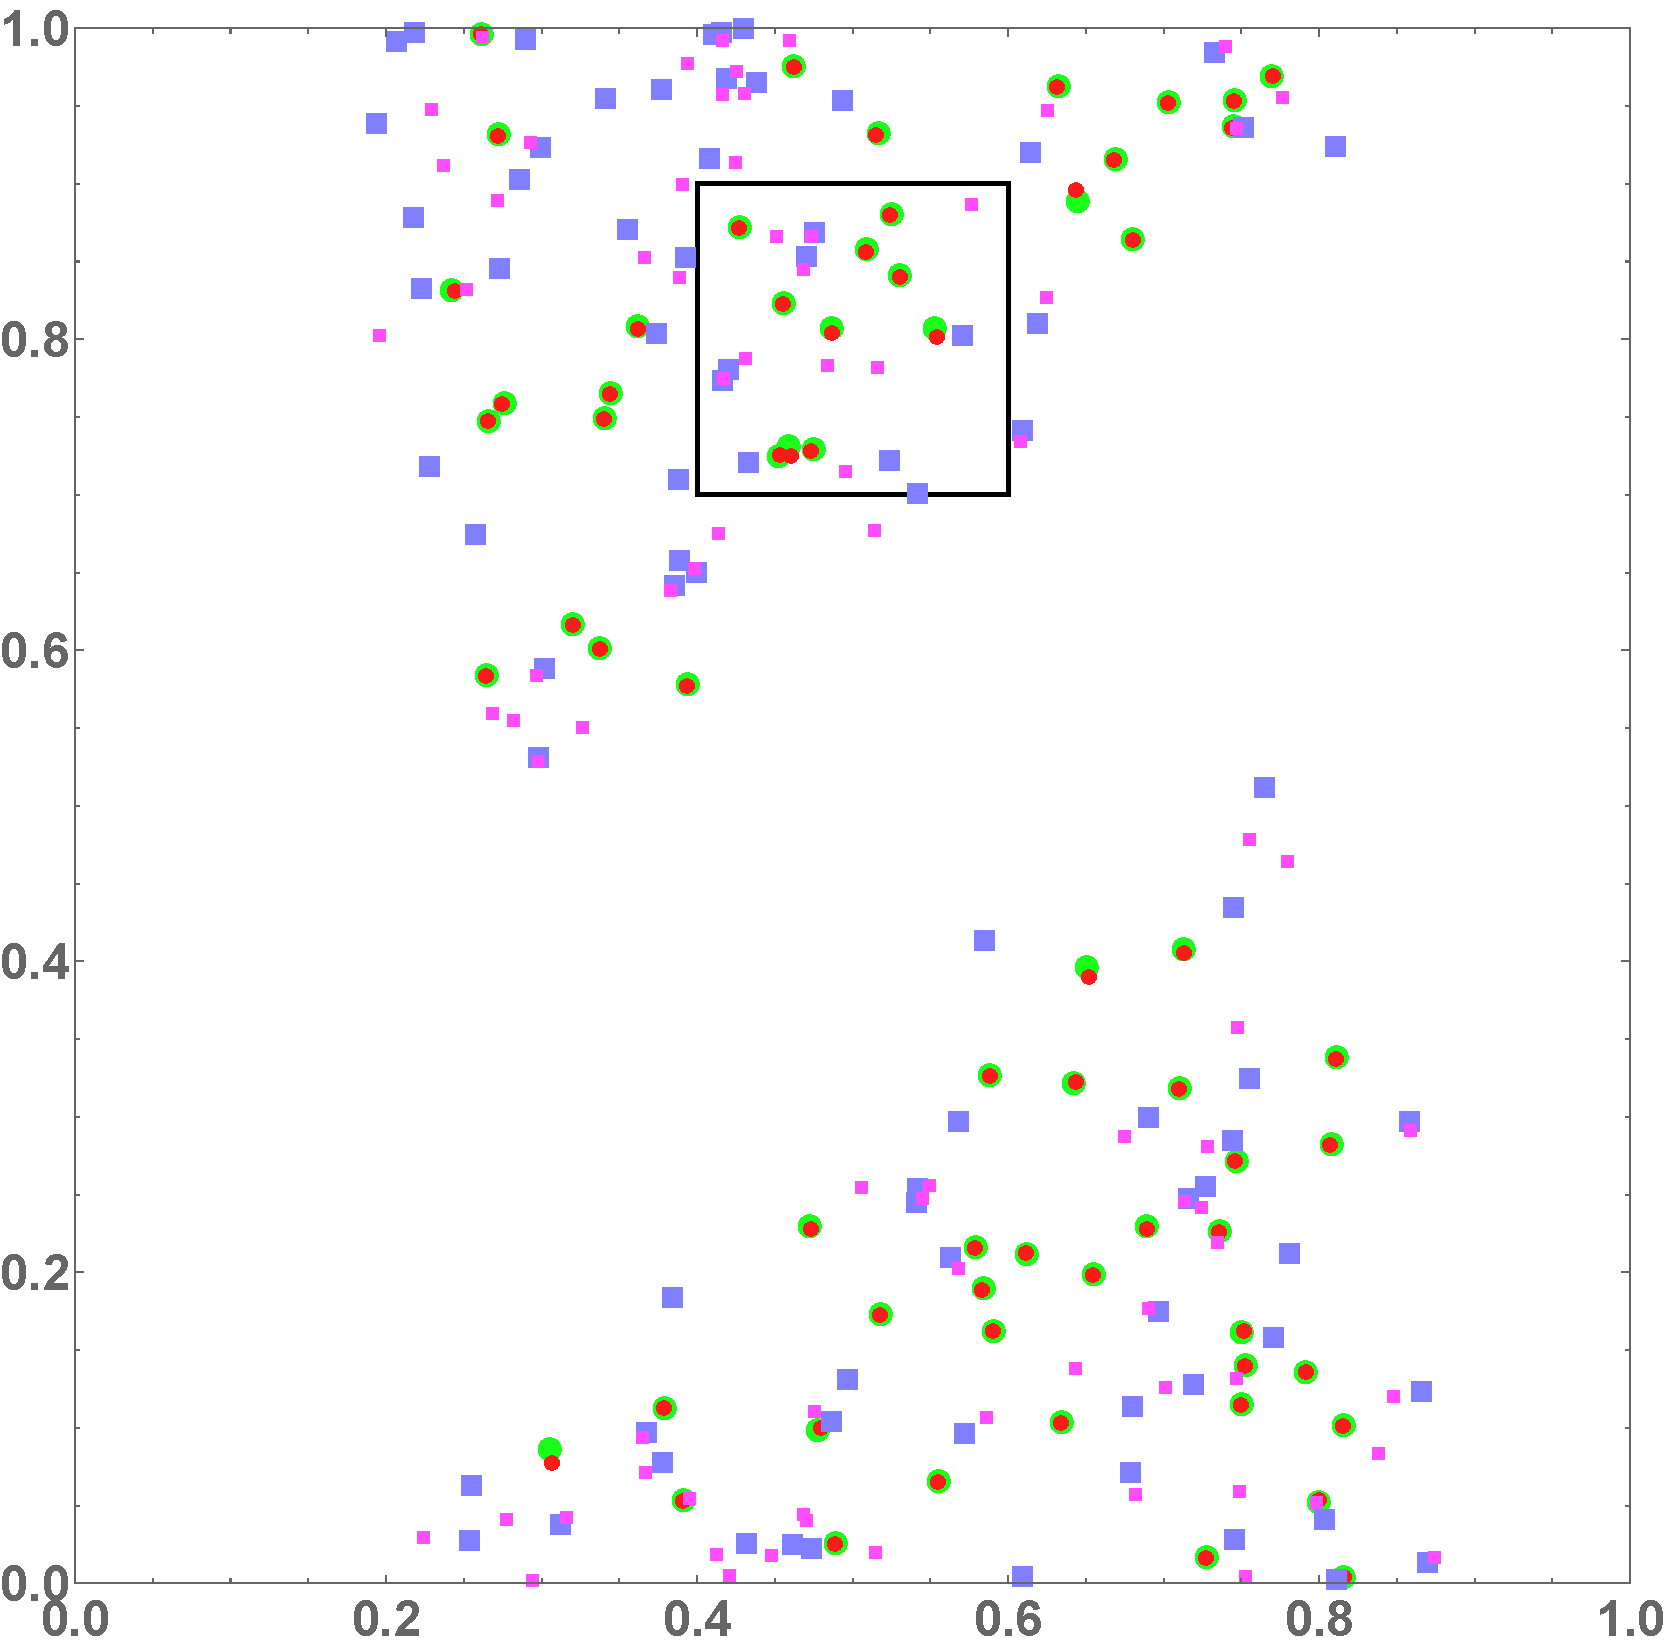
\includegraphics[width=0.42\textwidth]
{AKSs7BlockBorderG1}
\hspace{1ex}
(b) 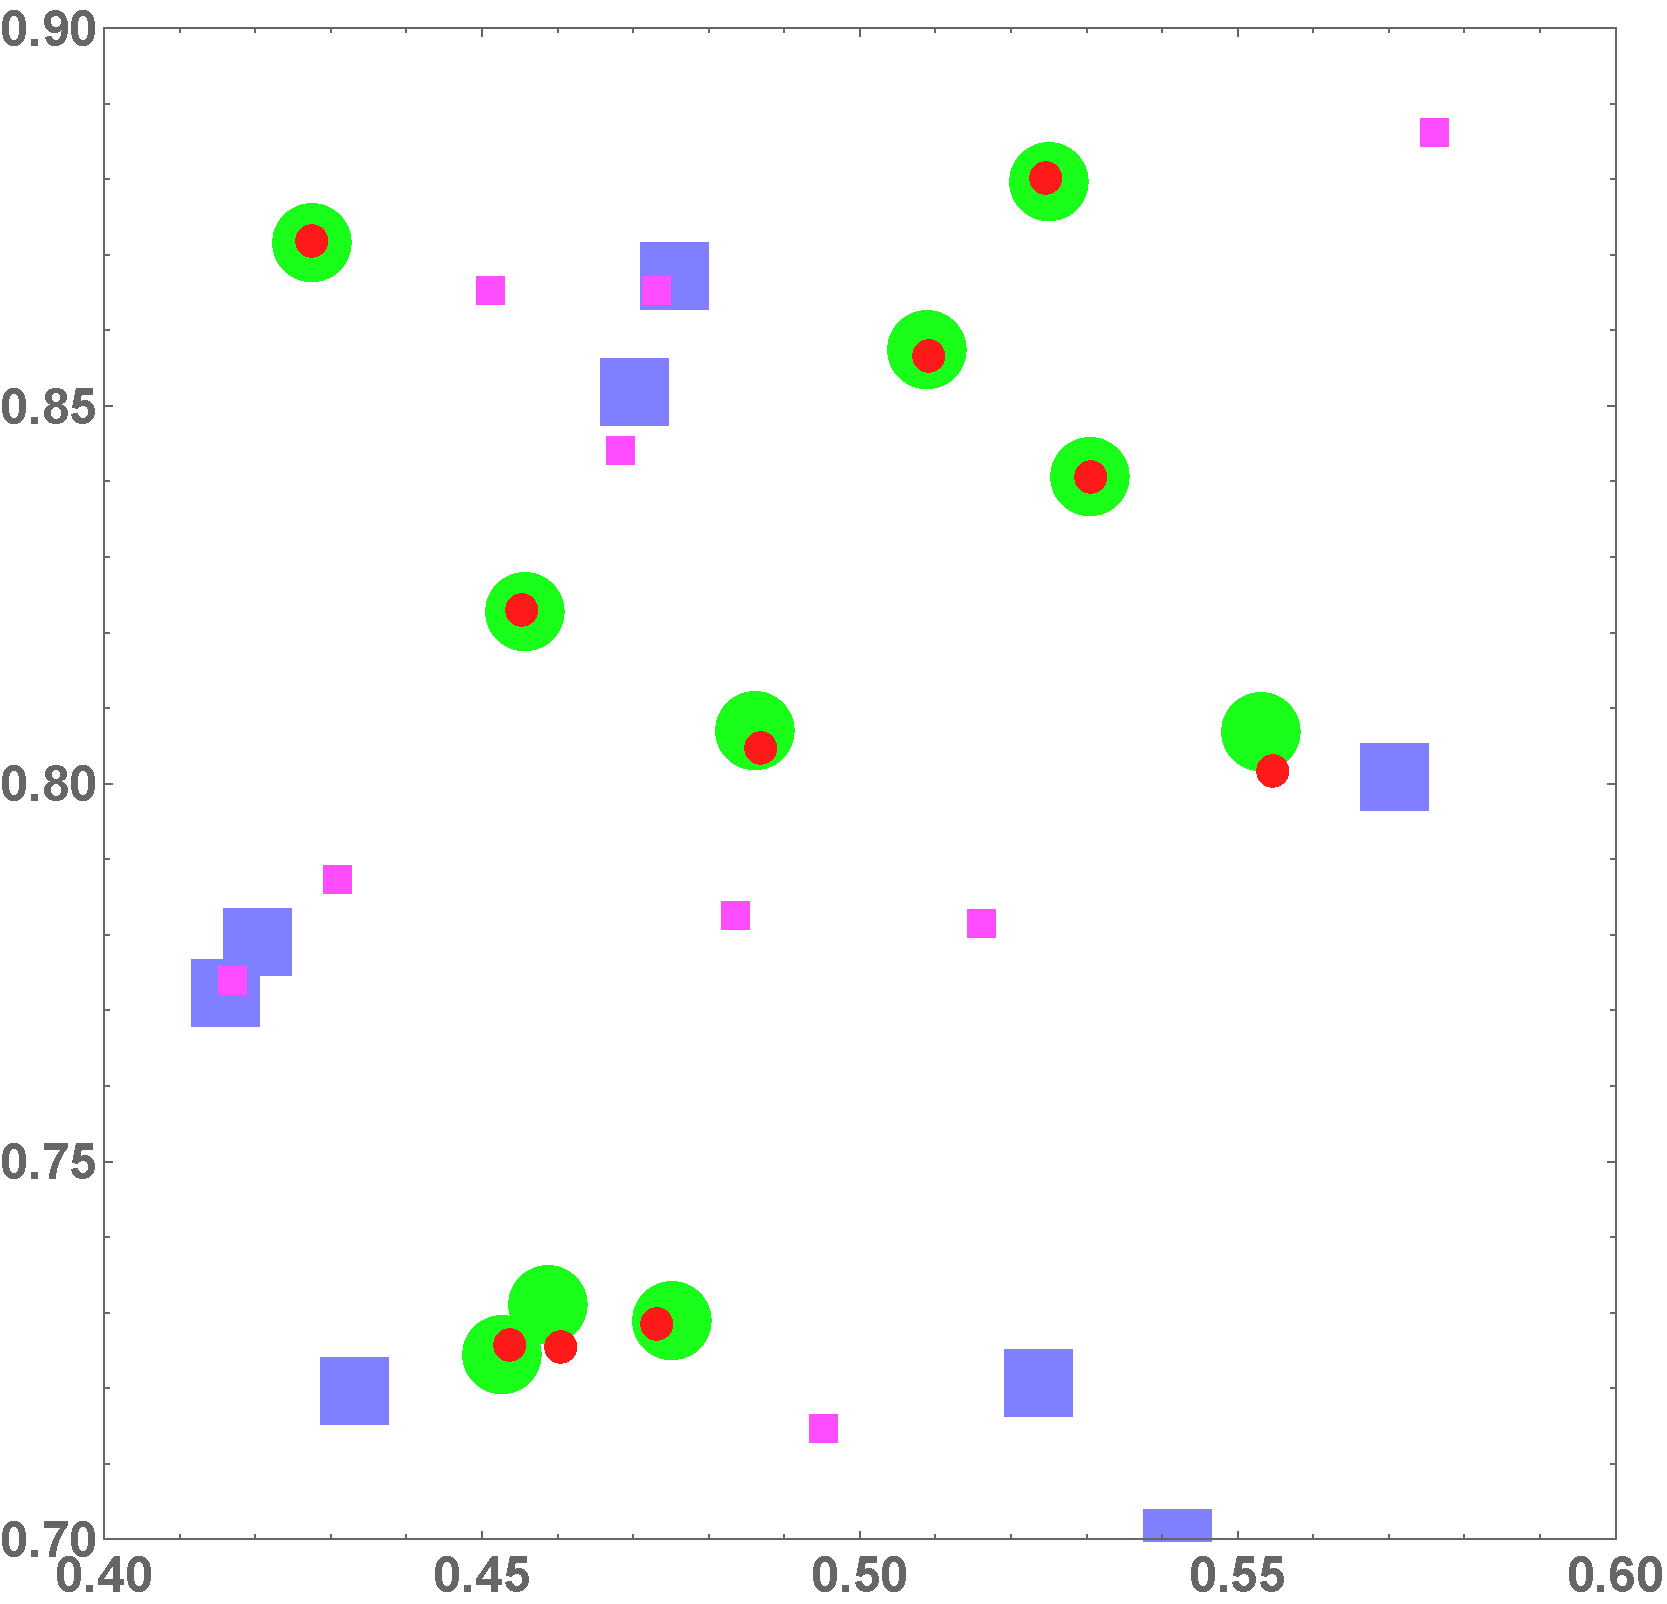
\includegraphics[width=0.43\textwidth]
{AKSs7BlockBorderG2}
\end{center}
\caption[]{
(Color online) (a) Phase space representation $(q^{(i)}_z,
p^{(i)}_z)$, where $i=1,2$  refers to the two \twots\ of
\reffig{fig:AKSsymbol}. (b) A zoom   into small rectangular area shown
on the left. The \statesp\ is covered only partially, as symbols in {\brick
s} $\Mm$ are restricted exclusively to the interior alphabet.
Only data for  $z=(n,t)\in \R$
are shown in the figure. The centers of red (small) circles  and green
(large) circles  are  the points $(q^{(i)}_z, p^{(i)}_z)$  of the first
($i=1$) and the  second ($i=2$) \twot\ for  $z$'s from the interior
$\R_{0}$. The centers of  violet (large)  and magenta (small) squares show
the respective points from   the border $\R_{1}$, see
\reffig{fig:AKSsymbol}. All
$(q^{(1)}_z, p^{(1)}_z)$ and $(q^{(2)}_z, p^{(2)}_z)$ in the interior
are well paired, while the separations are larger for $z$'s in the border region
$\R_{1}$.
This illustrates shadowing being exponentially stronger the closer the point is
to the center of \R, see \refeq{BGapprox}.
}
\label{fig:AKScloseActSp}
\end{figure}



% Did some re-label of some figures
\AKSpost{2019-08-28} {
I am re-generating both figures of \reffig{fig:BGcloseActSymb} with larger
periods in time and space ($L = 28$ and $T = 27$) so that they appear
more smoothly. I've also expanded the shadowing region so we could
observe an even larger exponential decay. Finally, I chose a coloring
pattern similar to that of Boris's paper\rf{GutOsi15}
\arXiv{1503.02676}. What do you guys think?\\ Here (on the blog/comments)
I am attaching the difference of symbols (check figure
\reffig{fig:AKSs7distupdated}).\\ For all the new figures I added, I've
labeled them identically to their previous version and re-labeled the old
ones "nameindex" so that they're stored in THE CLOUD.\\ Also I think it's
not needed to break down the region $\R$ into $\R_1, \R_2$ as we're no
longer distinguishing between outer and inner regions of shared symbols
(on figure 6,7  for example).
\\ \textcolor{blue}{(taken care of by AKS)}
}

\PCpost{2019-09-09} {
The point-wise \brick\ difference of \reffig{fig:AKSs7distupdated}
contains mo information - it's obvious from \reffig{fig:AKSLPS12} that
\(\Mm_{2,z}-\Mm_{1,z}\) is zero over \R.
}

\begin{figure}
\begin{center}
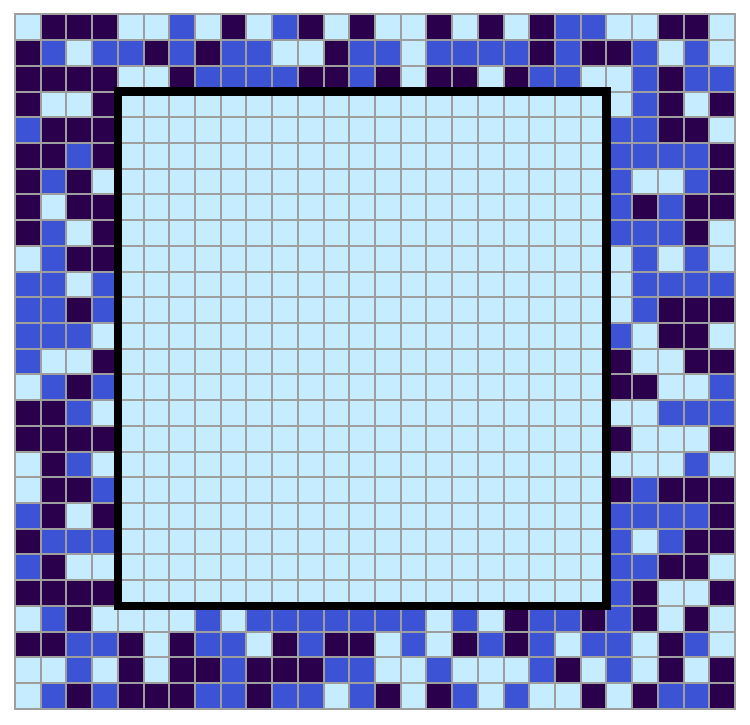
\includegraphics[width=0.45\textwidth]
{AKSs7distM1M2updated}
\end{center}
\caption[]{\label{fig:AKSs7distupdated}
%  AKS 2019-09-10 (Color online)
The site-wise distance \(\Mm_{2,z}-\Mm_{1,z}\) between the $[28 \times
27]$ symbol \brick s $\Mm_{1}$, $\Mm_{2}$ of \reffig{fig:BGcloseActSymb}.
(For a worse visualization, see \reffig{fig:AKSs7dist}.)
}
\end{figure}
%%%%%%%%%%%%%%%%%%%%%%%%%%%%%%%%%%%%%%%%%%%%%%%%%%%%%%%%%%%%%%%%%%%%%%%

\BGpost{2019-08-28} {:
\begin{enumerate}
        \item
\refsect{sect:intro}~{\em Introduction}: there were wide cuts in
comparison to the previous version. This was probably justified, but in
my opinion it is overdone by  now. It is difficult to understand what is
a general motivation for our paper. It looks very technical, dry and
restricted to concrete model.  A bit more poetry on (linear) coding,
e.g.,  why it is useful for description of dynamical systems might
improve things.
        \item
\refsect{sect:overview}~{\em Model and overview of the main results}: I
propose mother figures out how to use LaTex in order how to implement
several of my desired changes in today's so deftly emailed
\texttt{GHJSC16\_notes.pdf} (in yellow).

\end{enumerate}
    }


\PCpost{2019-08-29} {:
\begin{enumerate}
        \item
\refsect{sect:intro}~{\em Introduction}: I would like Boris to write the
general motivation in his own voice, as that is a voice that quantum
chaos community will resonate with. Predrag's pitch in the parallel
\refRef{CL18} universe is to the turbulence community, I think having the
two introductions, sung in different keys, will serve us better.
        \item
Text about not knowing the \PV\ cat map grammar rules is now
moved to just before
\refsect{sect:catLinGreen}~{\em From itineraries to orbits and back}.
\\
\refsect{sect:overview}~{\em Model and overview of the main results}
(Boris yellow markings) is reshuffled, hopefully as was his desire to
have had it reshuffled.
\end{enumerate}
    }


\BGpost{2019-09-07}{redundant, removed:
\\
\textbf{Answer to Q1.}
\textit{
The \catlatt\ admits a natural 2\dmn\  linear symbolic  code with a
finite alphabet. In principle, we can compute analytically the measure of
a given finite {\spt} symbol \brick\ ${\Mm_\R}$ over a region $\R$.
 }
 }

    \PCpost{2019-09-09} {
Files \emph{AKSLPS12\_2.pdf}, \emph{AKSLPS12\_3.pdf} are not referred to
anywhere. If needed, I think they corresponds to log difference of the
two small \twots\ of \reffig{fig:AKScloseActSymb}.
    }

%    \AKSpost{2019-09-10} {
%I have the two {\brick s} $\Mm'_1$, $\Mm'_2$ used to compute
%\reffig{fig:AKSLPS12}\,(b) stored on my laptop and if needed, I can add
%them to the blog.
%\\ \textcolor{blue}{\underline{AKS: taken care of, not needed.}}
%    }

    \PCpost{2017-09-04}{
Border notation in \refeq{inverseq} conflicts with
\refeq{DirichletGreenEquation}. Shouldn't it be
    \(
+\gd_{t,0}\ssp_0+\gd_{t,\ell+1}\ssp_{\ell+1}
    \)
    ?
    }
    \BGpost{2019-09-12}{
No way :)  I checked,  \refeq{inverseq} is correct.
    }
%\BGpost{2019-09-12}{Cannot swallow this:
%   \ie, it connects the partition boundary
%   at time 0 to the partition boundary at time $\ell+1$. }

 \PCpost{2017-09-25}{
Eq.~\refeq{catMapAverCoord} would be ``average coordinate'' for the
periodic boundary conditions, \ie, the periodic point (with repeats of
the defining \brick\ correctly summed. Here $\bar{x}_i({b})$ is at the
lower edge (lower corner?) of the admissible polytope.
    }
%\BG{2019-09-12}{You are right. Changed it to ``approximate coordinate''}


    \BGpost{2019-09-12 }{
I found the calculation following originally upon
\refeq{SingleCatJacobian} redundant, so I removed it to here. Hope you
understand everything without it.

The $\pS_b$ are partitions of the $(\ssp_{0},\ssp_{1})$ \statesp, in
contrast to the polygons $\Pol_{b}$, plotted in the Lagrangian
coordinates $(\ssp_0, \ssp_{\ell+1})$, see \reffig{fig:PairSymbol}. Hence
the interior alphabet measures $\Msr(b)$, $\Ssym{i}\in\Ai$, are given by
the Jacobian \refeq{SingleCatJacobian} of coordinate transformation from
the Lagrangian coordinates $(\ssp_0, \ssp_{\ell+1})$ to the \statesp\
$(\ssp_0,\ssp_1)$,
\(
\Msr(b) = {U_{|b|}({s}/{2})}^{-1}
\,.
\)
The value of $U_{|b|}({s}/{2})$ is always an integer greater than 1,
and thus the $(\ssp_{0},\ssp_{1})$  \statesp\ is ``magnified" and wrapped
around the $(\ssp_0, \ssp_{\ell+1})$ \statesp\ $U_{|b|}({s}/{2})$
times through $\ell$ iterations of the cat map.
Lagrangian coordinates $(\ssp_0,\ssp_{\ell+1})$  are related to \statesp\
coordinates $(\ssp_k, p_{k})$,
\(
p_t = (\ssp_{t} - \ssp_{t-1})/\Delta t \,,
\)
at time $t \in (0, \ell+1)$ by
\begin{eqnarray}
 & x_t &=  \bar{x}_t({b}) +
          \frac{U_{\ell-t}(\frac{s}{2})}{U_{\ell}(\frac{s}{2})}\,\ssp_0
                +
          \frac{U_{t-1}(\frac{s}{2})}{U_{\ell}(\frac{s}{2})}\,\ssp_{\ell+1}
\continue
 & p_\RJedit{{t+1}} &= \bar{x}_{t+1}({b}) -\bar{x}_t({b}) +
          \frac{U_{\ell-t-1}(\frac{s}{2})
               - U_{\ell-t}(\frac{s}{2})}{U_{\ell}(\frac{s}{2})}\,\ssp_0
          +\frac{U_{t}(\frac{s}{2})-U_{t-1}(\frac{s}{2})}{U_{\ell}(\frac{s}{2})}\ \ssp_{\ell+1}
\,.
\nonumber %\label{SquareCut3}
\end{eqnarray}
This is a linear map, so its Jacobian
\(
d_\ell =
   {|\partial (\ssp_0, \ssp_1)}/{\partial (\ssp_0, \ssp_{\ell+1})|}
\)
is simply
\RJedit{
\bea
  d_\ell
%  &=& \frac{\partial (\ssp_0, \ssp_1)}{\partial (\ssp_0, \ssp_{\ell+1})}
  &=& \frac{1}{U_{\ell}(\frac{s}{2})^2}
  \det
   \left(\begin{array}{cc}
  U_{\ell}(\frac{s}{2})  & U_{-1}(\frac{s}{2}) \\
   U_{\ell-1}(\frac{s}{2})  & U_{0}(\frac{s}{2})
  \end{array} \right )
= %\continue &=&
  \frac{1}{U_{\ell}(\frac{s}{2})}
\,.
%\label{SingleCatJacobian}
\eea
}
        }


    \PCpost{2019-09-12 }{Droped this: ``
Unlike the systems studied in \refref{BunSin88}, \catlatt\ cannot be
conjugated to a product of non-interacting  cat maps. A way to see that is, for an example, to
compare the numbers of \po s in the two cases -- they differ.''
    }

            \BGpost{2017-09-14}{
    More  straightforward argument is that $\mathcal{B}_{\scriptscriptstyle L}$ (see
    \refeq{LperHamiltonian} in \refappe{sect:HamiltonCatLatt})  is not
    conjugated to any feline  with  $B=0$).
%    I would not even bring symbolic dynamics issue at
%    this point because symbolic dynamics is a matter of choice. Even if the
%    two maps  are conjugated you can always introduce different/unrelated
%    symbolic dynamics by using whatever partitions.
    }

    \BGpost{2019-09-27}{
Checked \refeq{DirichletGreenEquation}. It is OK. The only question is
whether the notation is sufficiently explained? (I plan to improve a bit
\reffig{fig:block2x2}.)
    }

    \PCpost{2019-09-28} {
% \PC{2019-09-28} rechecked all the blocks
Has anybody checked that the \brick\ of example following
\refeq{2dCatLattAlph7} is admissible?
    }
    \BGpost{2019-09-30} {
Most probably not. On the other hand it is not terribly important. At the
worst case they are all zeroes :)
    }
    \PCpost{2019-10-08} {
Cannot beat the post-Soviet perfectionism :)
    }

        \BGpost{2019-09-30} {
We need Hamiltonian formulation for two reasons. First, our measure
$dp\,dq$ comes from there. Second,  for all   numerics we actually use
initial data problem i.e., Hamiltonian formulation. We need
\refappe{sect:HamiltonCatLatt}, but should keep it compact.
        }

        \BGpost{2019-10-03} {
A risky statement below. Did anybody checked this?
``As $\Xx_{z}$ take rational values for any finite $[L\!\times\!T]$ \twots,
for sites sufficiently close to the center of \R\ the
cancelation $x_{2,z}-x'_{z}$ can be exact.''
{\bf Predrag}: dropped it.
        }

%%%%%%%%%%%%%%%%%%%%%%%%%%%%%%%%%%%%%%%%%%%%%%%%%%%%%%%%%%%%%%%%%%%%%%%%
    \PCpost{2017-01-25} {
Gutkin and Osipov
refer to the map generated by the action \refeq{GutOsi15_3.1:action} as
non-perturbed \textit{coupled cat map},
and to an \twot\ $p$ as a ``many-particle periodic orbit'' (MPO) if
$\ssp_{nt}$ is doubly-periodic, or ``closed,'' \ie,
\beq
\ssp_{nt} = \ssp_{n+L,t+T}
    \,,\quad
n = 0,1,2,\cdots, L-1
    \,,\;\;
t = 0,1,2,\cdots, T-1
    \,.
\ee{GutOsi15po2D}
Action of an \twot\ $p$ is
\beq
S_{p}=-\frac{1}{2}\sum_{t=1}^T\sum_{n=1}^L \Ssym{nt}\ssp_{nt}
\,.
\ee{GutOsi15_3.1:action}
    }
    \BGpost{2019-10-08} {
Do you want  formula for action in the paper?}
    \PCpost{2017-01-25} {
Not unless it is necessary to discuss it anywhere in the paper...
Besides, to me \refeq{GutOsi15_3.1:action} seems almost
surely wrong.}
%%%%%%%%%%%%%%%%%%%%%%%%%%%%%%%%%%%%%%%%%%%%%%%%%%%%%%%%%%%%%%%%%%%%%%%

    \PCpost{2019-01-24}{
    Some of this \twot\ stuff presumably goes to the kittens paper\rf{CL18};
    this paper does only the Dirichlet b.c..
        }
    \BGpost{2019-10-08}{
Do you mean $\gp_{zz'}$? Should we refer here to \rf{CL18} instead of
\refappe{sect:Green}?
    }

        \LHpost{2017-09-05}{
I'm looking at numerical data. The number of total {\admissible} rules of
{cat map} takes an exponential law: $\sim 2.63^n$ for s=3, $\sim 3.74^n$
for s=4 for example. i.e., effectively 2.63/3.74 symbols are needed for
s=3/s=4. They agree with that from the topological entropy and Lyapunov
exponent, which are $(3+\sqrt{5})/2, 2+\sqrt{3}$, respectively.
Intuitively this should hold (that $\log[$~number of {\admissible}
rules]/n = topological entropy), but is it well-known/justified in
symbolic dynamics?
        }
    \BGpost{2019-10-10}{
Now dealt with, in \refsect{sect:catEntropy}. Added concrete numbers to
the picture caption.
    }

%%%%%%%%%%%%%%%%%%%%%%%%%%%%%%%%%%%%%%%%%%%%%%%%%%%%%%%%%%%%%%%%%%%%%%%%
    \BGpost{2017-07-31}
{Should we change layout of \reftab{tab:RJpruning} to the horizontal one? }
    \PCpost{2017-08-11}
{Not sure - easier to see the exponential growth in this format.}
    \LHpost{2017-09-01}{
How about including list of new pruning rules for small lengths as an Appendix?
        }
    \BGpost{2019-09-14}{Would be fine if you can do this.}
%%%%%%%%%%%%%%%%%%%%%%%%%%%%%%%%%%%%%%%%%%%%%%%%%%%%%%%%%%%%%%%%%%%%%%%%

%%%%%%%%%%%%%%%%%%%%%%%%%%%%%%%%%%%%%%%%%%%%%%%%%%%%%%%%%%%%%%%%%%%%%%%%
    \BGpost{2017-08-02} {
\reffig{fig:AKSs13TwoBlock1}
``Any
$4\times 4$ {\brick} of symbols appears one and the same number of times
in both representations.''

means the following: If we scroll/peep  through the
(upper)  torus symbolic representation  with $4\times 4$ window, there
are exactly $NT$ different  $4\times 4$ \brick s of symbols.  Each of
them appears the same number of times, as well,  in the symbolic
representation of the bottom  tori (but for  possibly  different window
positions).
     }
%%%%%%%%%%%%%%%%%%%%%%%%%%%%%%%%%%%%%%%%%%%%%%%%%%%%%%%%%%%%%%%%%%%%%%%%

    \PCpost{2019-10-19}{to Boris and Han:
I have not checked it, but \refeq{SpatiotemporalEntropy} is very pretty,
kind of formula on gets from discrete-Fourier digitalization of Green's
functions. You seem to be saying the $\det$ of the 2-torus Jacobian
matrix counts the numbers of \twots, and are computing $\ln\det$ to get a
rate per area $|\R|$. Could some Chebyshev polynomials lurk  here, and an
analytic answer?
    }

    \PCpost{2017-09-14}{
\catLatt\ metric entropy \refeq{AsymJacobian} is presumably exact for
\catlatt\ as long as \period{} and \speriod{} are going large at
comparable rates. For systems without the space-time symmetry
$t\leftrightarrow{x}$, $h_k$ should be different along the time and
the space directions, so I do not think we can define one spacetime entropy?
Enlightenment on this point would be very welcome.
    }

    \AKSpost{2019-10-20}{to Predrag and Boris:
I can see why we would want to plot the logarithm of the site-wise
distance \(\ln|x_{z}-x'_{z}|\) between the states $\Xx$, $\Xx'$. The idea
would be to remain in the Lagrangian picture. To be clear, right now:
\begin{itemize}
\item
\reffig{fig:BGcloseActSymb} is actually plotting \(\ln \left( \sqrt{(q_z
- q'_z)^2 + (p_z - p'_z)^2} \right) \) which is the site-wise distance in
the Hamiltonian picture ($q = x$ and $p$ is momentum). I already have
generated the figure that corresponds to the Lagrangian site-wise
distance, which is simply  \(\ln|x_{z}-x'_{z}|\). We want that one,
correct?
\item
for \reffig{fig:AKSs13TwoBlock} and \reffig{fig:AKSs13TwoBlock1}, I can
also generate the same 'Lagrangian' distance. For the 3 diamond
blocks, we would have to generate two site-wise distance, let's say
between $(\Xx_1, \Xx_2)$ and $(\Xx_1, \Xx_3)$. Would that work? It would
look something like what's on figure G11 of this blog.
\end{itemize}
\textcolor{blue}{(taken care of by AKS)}
    }

    \PCpost{2019-10-20}{to Boris -
I admit to not understanding to what the title of
\refsect{sect:fullShade}~{\em Full shadowing} refers to. $\Xx_i-\Xx_j$
shadow each other with the doughnuts, as they should, all distances
elsewhere are of O(1). What's {\em Full shadowing} about that?
    }

    \PCpost{2019-10-20}{
I would like to give shelter to \reffig{fig:AKSs13TwoBlock} and
\reffig{fig:AKSs13TwoBlocks1} here in Bloglandia - they would require too
much explanation - and replace them by the likes of
\reffig{fig:AKSdslp12}. We could replace both by a single figure, the
left frame giving \(\ln|x_{z}-x'_{z}|\) for \reffig{fig:AKSs13TwoBlock},
and using \reffig{fig:AKSdslp12} as the right frame, no need to exhibit
the two other pairwise distances, as they should all look very much the
same.

We let Boris decide.
\\ \textcolor{blue}{(taken care of by AKS)}
    }

    \PCpost{2019-10-19} {
Green's function notation is $\gd_{t}$ is not helpful - it's a matrix, so
easier to use $\gd_{tt'}$ throughout.
Green's function notation is $\gd_{nt}$ is not helpful, and here even
misleading - it's a tensorial matrix, so less confusing to use $\gd_{zz'}$
notation throughout.
    }
\BGpost{2019-10-21}
{ Semi-agree :). It is a matter of perception - after all ``Green's
function`` is also (or rather first of all) a function (of $z,z'$).   I
have changed the notation. Looks more clumsy, but might be a less evil.
}

    \PCpost{2016-11-08} {
Say: THE BIG DEAL is

for $d$\dmn\ field theory, symbolic dynamics is not one temporal sequence
with a huge alphabet, but $d$\dmn\ {\spt} tiling by a finite alphabet

``Classical foundations of many-particle
quantum chaos'' I believe could become a game-changer.
Corresponding dynamical zeta functions should be sums over {\twots} (as
is done in the kittens paper\rf{CL18}), rather than $1$\dmn\ \po s.
    }
    \BGpost{2016-11-20} {
All papers that I know were dances around question of uniqueness SRB measure.
Either show that measure is unique or opposite way around (phase
transitions). We know from the start that system is in the high temperature
regime, so the measure is unique.
    }


\BGpost{2019-09-12}{Two remarks
\begin{enumerate}
  \item
In several  cases you call $\Ai$ as a ``full shift''.
This looks wrong. As far as I understand
(see \HREF{http://www.scholarpedia.org/article/Symbolic\_dynamics}
{Scholarpedia}),
one can call $\Ai^\integers$  (together with the shift map $\Tshift$)  as
a ``full shift'', but not $\Ai$. ``Full shift'' is
a dynamical system = state space ($\Ai^\integers$) + map (shift) not just
alphabet.
  \item
Regarding notion of generating partition.
``A partition Q is called a generator or generating partition if
 $\Msr$-almost every point x has a unique symbolic name''.
 So the partitions which we consider here are generating.
 I think what you mean by ``generating''  are  rather called
 ``Markov partitions''.
\end{enumerate}
{\bf Predrag 2019-09-17} Thanks, for me these are very important remarks,
to be fixed also in ChaosBook. Will chew on them... Until then,
keep this remark here, as a reminder.
       }

    \PCpost{2019-10-19} {
I would like to use only one Green's function notation, \ie, $\gp_{zz'}$,
and not $\gd (z,z')$.
    }
    \BGpost{2019-10-19} {
Do you mean $\gd_{zz'}$ ($\gp_{zz'}$ is reserved for periodic boundary
conditions)? I have changed $\gd (z,z')$ to $\gd_{zz'}$, everywhere
except section A3. Seems to me - putting there everything downstairs
would make things  more  uglier.
    }


   \BGpost{2019-09-30}{
To be on the safe side it would be nice to check if everything above is
compatible with numerics on \reffig{fig:RJsymbol}. Is there a hero who
can do this?
    }

     \PCpost{2019-10-20}{
to Boris: A typical reader (if there will be any:)) of this opus magnum
will not be encumbered by precisely your flavor of your quantum chaos
baggage. To motivate this funky section full of peculiar doughnuts and
their permuted holes, you need to explain why action differences (are the
defined anywhere?) need to be small for close \po\ encounters in the
quantum work that connects \po s and quantum chaos spectral
distributions.
    }

\BGpost{2019-10-26}{
It was done already in our paper with Vladimir. No need to repeat.
Motivation here is somewhat different - By using internal symbols you can
easily  manufacture \twots\ with whatever   properties you wish/need (like
in baker's map).
    }

    \BGpost{2019-10-26}{

1) Brought 2 unnamed figures back from the exile  (at least they are correct).

2) Removed some confusion over domains -- $\ZLT$ and $\R$ are 2 different
domains. $\R$ is sub domain of $\ZLT$. Removed some unnecessary/confusing
indexes

3) If you start to change notation (I prefer not to do this  at this
stage) - be careful there is high probability you will need to do it all
over the paper  = lot of work.

4)
Did  not like `doughnut'  slang - everything is pretty flat here (You can
sell some topological stuff  but only after very long and unnecessary :)
discussion = you would need first to make a smooth picture out of this
i.e., discuss smooth field theories. Some attempts in this direction are
in our paper with Vladimir.)   `doughnut hole' is completely misleading.
So for  the lack of anything better I return back to 'annular-like
domain'  = seems to me much less evil.
\\ \textcolor{blue}{(taken care of by AKS)}
    }

    \PCpost{2017-09-06} {to Boris:
Do you have some analytically small number, like $\Msr(\MmR)= 1/8!s(s^2-1)$
for any of the measures in \refsect{sect:2Dnumerics}?
    }
    \BGpost{2019-09-30}
{To Predrag: for this particular $\Mm$  would be a lot of work to get it.}


    \BGpost{2019-10-28}{
Returned \reffig{fig:AKSdslp12} back to Blogosiberia
%%%%%%%%%%%%%%%%%%%%%%%%%%%%%%%%%%%%%%%%%%%%%%
\begin{figure}
\begin{center}
(a) 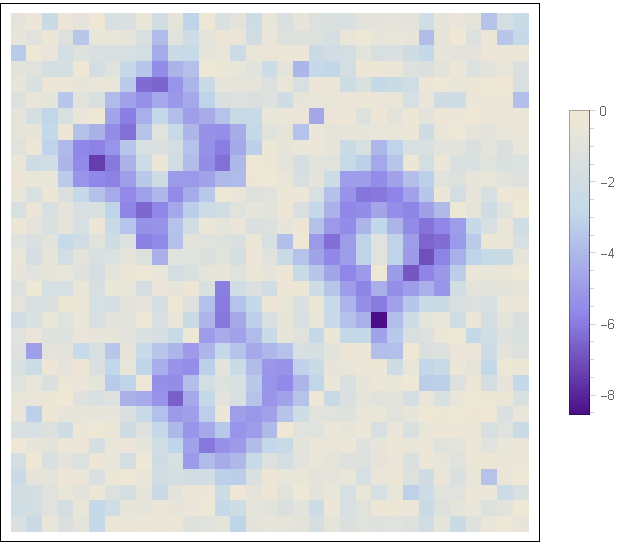
\includegraphics[width=0.45\textwidth]{AKSdslp12}
(b) % \includegraphics[width=0.45\textwidth]{AKS???}
\end{center}
\caption{\label{fig:AKSdslp12}
(Color online) The plots of the logarithm of the site-wise distance \(\ln|x_{z}-x'_{z}|\)
(a) of the states $\Xx_1$, $\Xx_2$ of \reffig{fig:AKSs13TwoBlock}
illustrate the exponential fall-off of the site-wise distances within
the shared doughnut \brick s $\Mm_{\R_1}$, $\Mm_{\R_2}$;
(b) of one of the three pairs of states $\Xx_i$, $\Xx_j$ of
\reffig{fig:AKSs13TwoBlock2}; the other combinations have similar
site-wise distance plots. Outside of the shared domains the distances
are of the order $1$.
    \AKSedit{2019-10-30 Boris: ``completely wrong!''}
    }
\end{figure}
%%%%%%%%%%%%%%%%%%%%%%%%%%%%%%%%%%%%%%%%%%%%%
        }

%    \AKSpost{2019-10-28}{
%Some of the figure referencing has been compromised:
%\begin{itemize}
%\item
%Right now, \reffig{fig:AKSs13TwoBlocks} and \reffig{fig:AKSs13TwoBlocks1}
%refer to appendix figures but should be figures 9 and 11 of the main.
%\item
%The sentence starting with "In figures ... and ... we illustrate these
%parings.." should be figures 9 and 11 of the main and not
%\reffig{fig:AKSs13TwoBlocks} \reffig{fig:AKSs13TwoBlocks1}.
%\item
%The figure mentioned in the caption of figure 11 of the main should be
%\reffig{fig:AKSs13TwoBlock2}. I actually fixed that one. Please approve
%these changes.
%\end{itemize}
%{\bf 2019-10-29 Predrag} Boris seems to have fixed all of these suggestions
%already?
%\\ \textcolor{blue}{(taken care of by AKS)}
%    }

     \PCpost{2017-08-06} {
I have crosschecked \refeq{exactBlock1x1} with
\emph{siminos/spatiotemp/reportRJ.tex}
    }

    \PCpost{2017-09-06} {to Rana - explaining \reffig{fig:RJsymbol} you write:
``relative frequency equal to 0.995755'': how many digits do we trust? we
should state only the significant digits.

 When you replot, and replot you must, make both plots in
\reffig{fig:RJsymbol} square, with both axes going from 0 to 1.
    }

    \PCpost{2016-11-07}{
% Explain in the caption of \reffig{fig:PairSymbol}:
\reffig{fig:SingleCatPartit}:
Note 5th bullet on \refpage{sect:NonlinTips} and \refappe{figinc}.
\\
Refer here (within this comment) to the source code (in the repository) that
generates these figures.
\\
{\bf 2019-10-29 Predrag} giving up waiting on the response.
    }
    \PCpost{2017-09-04}{
to Li Han or Adrien or Rana:
Please reformat the LaTeX layout of \reffig{fig:SingleCatPartit} (not the
plots themselves! and without decreasing the sizes of individual plots)
so each plot has in the lower left corner a label (a), (b), ..., (h), (i)
\\
{\bf 2019-10-29 Predrag} giving up waiting on the response.
        }

    \PCpost{2019-09-30}{
In \reffig{fig:AKSs13TwoBlock} Boris writes ``the two \twots\ $\Xx_1$ and
$\Xx_2$ shadow each other at every point.'' I do not know what ``every
point'' he has in mind, but I agree that $\Mm_1$ and $\Mm_2$ are
identical everywhere except for the $A_1$, $A_2$ permutation, so if I
stand on my head, I can see it being right in some inexplicable sense.

Happy is the referee who grasps \reffig{fig:AKSs13TwoBlocks} without any
reference to any explanatory text.
    }
    \AKSpost{2019-10-28}{
I don't know to what extent do Predrag wanted to explain or define
the use of momentum coordinates in \reffig{fig:AKSs13TwoBlocks} and
\reffig{fig:AKSs13TwoBlocks1}. I
am satisfied with its current state, but could see that we add the
definition for the coordinates $(q^{(i)}_z, p^{(i)}_z)$.
\AKS{2019-10-30}{Those are defined in \refappe{sect:HamiltonCatLatt}}
    }
    \PCpost{2019-10-29}{
Explanation would be nice... When I write in \reffig{fig:AKSs13TwoBlocks}
caption that ``This Hamiltonian representation is explained in
\refappe{sect:HamiltonCatLatt}'' I am lying, no?
\AKS{2019-10-30}{Not sure about that...}
    }

    \AKSpost{2019-10-30}{
Added a \textcolor{blue}{(taken care of by AKS)} note to each completed
blog post which concerned \refsect{sect:twots}.
% I am pretty sure you can remove
% \reffig{fig:AKSdslp12} since Boris said it was completely wrong.
    }

   \RJpost{2019-09-30}{dropped this: ``
If only a column or row of
symbols belongs to the interior alphabet,
the  value of
relative frequency $|\Pol_{\MmR}|$ is typically either  close to $1$ or  $0$.
For example, for
$s=7$
the \brick\
\[
        \left[\begin{array}{cc}
        5 & {3} \\
        \underline{1} & 0
              \end{array}\right]
\,,
\]
with the $[3,0]^T$ column in the interior alphabet,
has a relative frequency $\approx 1-0.005$. % was 0.995755.
''
    }

\PCpost{2016-10-10}{RECHECK! Do they still use pacs?}

     \BGpost{2017-08-31} {
 On my current level of resolution (5 in the morning)
%everything is
%perfect except labels  at x-axis of \reffig{fig:RJsymbol}\,(c) and (d).
%Probably  should be $\gamma -3$ (without 1) under condition you move
%point in \refeq{block2x2bases=3} one step right.
%%Also word ``decimal" should be erased from the earth (or at least from
%%the caption and near \refeq{block2x2bases=3}.
%% On p. 6 (down) probably ``requires AN extensive use  of ..."
%Otherwise
the paper is completely ready for submission  at any journal of this
galaxy.
    }
\end{description}

\subsection{Cats/nonlin-v2/  GHJSC16 revisions}
\label{sect:GHJSC16blogV2}
\begin{description}

     \BGpost{2020-10-16} {dropped formulas\\
The remarkable feature of the {\catlatt}  is that its every solution
\(
\{\ssp_{z},  z\in \integers^{d}  \}
\)
is uniquely encoded by a linear transformation to the corresponding finite
alphabet $d$\dmn\ symbol lattice
\(
\{\m_{z}, z\in \integers^{d}\}
\)
    }

     \BGpost{2020-10-16} {dropped formulas\\
dropped:\\
This paper builds explicit 2\dmn\ {\catlatt} \statesp\ partitions using
winding numbers  \(\m_{z}\). An alternative, generating \AW\ partition
for the cat map, and a \po\ theory for \catlatt\ in higher dimensions are
formulated in the parallel paper\rf{CL18}.

inserted instead later:\\
\edit{
This paper builds explicit 2\dmn\ {\catlatt}   symbolic dynamics  using
winding numbers  \(\m_{z}\). (An alternative construction, based on
generating \AW\ partition for the cat map, and a \po\ theory for
\catlatt\ in higher dimensions are formulated in the parallel
paper\rf{CL18}.)
    } %end \edit
        }

     \PCpost{2020-10-17} {
Removed:\\ ``(An alternative construction, based on  generating \AW\ partition
for the cat map, and a \po\ theory for \catlatt\ in higher dimensions are
formulated in the parallel paper\rf{CL18}.)''

The case $s<-\edit{2}$ can be treated analogously.
        }

     \BGpost{2020-10-16} {added:\\
\edit{
The following theorem allows  for evaluation of symbol blocks measures.
\begin{theorem}
Let $b$ be a finite sequence of symbols.  The corresponding  measure  is
given by the product
\beq
 \Msr({b}) =d_\ell |\Pol_{b}|,  \qquad  d_\ell =
  {1}/{U_{\ell}({s}/{2})},
\ee{FreqDecompBlog}
where
 $|\Pol_{b}|$ is  the area of the polygon $\Pol_{b}$
defined  by the inequalities
\begin{eqnarray}
 & 0&\leq \bar{x}_i({b})
     +\frac{U_{\ell-i}(s/2)}{U_{\ell}(s/2)}\ssp_0
     +\frac{U_{i-1}(s/2)}{U_{\ell}(s/2)} \ssp_{\ell+1}<1
     \,,\qquad i=1,\dots ,\ell,
\label{SquareCut1blog} \\
 & 0&\leq \ssp_0 <1, \qquad  0\leq \ssp_{\ell+1} <1
 \,
\label{SquareCut2blog}
\end{eqnarray}
in the plane $(\ssp_0,\ssp_{\ell+1})$.
\end{theorem}
    }
} %end \edit

     \PCpost{2020-10-16} {
Boris has now renamed  refeq~{FreqDecomp} to \refeq{FreqDecomp1}. While
Boris-introduced \refeq{FreqDecomp} is cited many times, \refeq{FreqDecomp1}
is never cited.

Too many `In general,'s

mark as EDITED:\\
Since all coefficients in  (\ref{SquareCut1})  are given by rational numbers,
the polygon areas $|\Pol_{{b}}|$ are rational too. The same holds for the
$d_\ell$ factor. As a result,   measures  $\Msr({{b}})$ are always rational
(see, for example, \reftab{tab:RJ2letFreq}). This allows for their exact
evaluation by integer arithmetic.  As the factor $d_\ell$ in \refeq{FreqDecomp} is known explicitly, the
    }

     \BGpost{2020-10-16} {rewrote:
\paragraph{Interior symbols.}
For \brick s composed of interior symbols only, the inequalities
(\ref{SquareCut1})  are always satisfied, and  $\Pol_{{b}}$ are unit
squares of area $1$. The corresponding measure
\[
\Msr({b})
= {1}/{U_{|{b}|}({s}/{2})}, \qquad  \Ssym{i}\in \Ai
\,, \quad  i=1,\dots |{b}|
\]
depends  only  on the length of the \brick\ ${b}$.

\paragraph{Rationality.}
Since all coefficients in  (\ref{SquareCut1})  are given by rational numbers,
the polygon areas $|\Pol_{{b}}|$ are rational too. The same holds for the
$d_\ell$ factor. As a result,   measures  $\Msr({{b}})$ are always rational
(see, for example, \reftab{tab:RJ2letFreq}). This allows for their exact
evaluation by integer arithmetic.
    }

     \PCpost{2020-10-31} {
Dropped: `` The always trustworthy but so un-cited Soviet scientists
(1781–1840) teach us that...'
    }

     \PCpost{2020-10-17} {
Edited everything down to $d=2$ dimensions. Was:\\
The \templatt\ map \refeq{eq:CatMapNewton1}, and the \catlatt\
\refeq{eq:CatMapNewton2} can be brought into uniform notation  and
generalized  to $d$ dimensions by converting the {\spt} differences to
discrete derivatives. This yields the discrete screened Poisson
equation\rf{Dorr70,HuCon96} for the $d$\dmn\ {\em \catlatt}.

The key insight  is that  {\em $d$\dmn} {\spt}
 lattice of integers
\(
\{\m_{z}\} = \{\m_{z}, z\in \integers^{d}\}
\)
is the natural encoding of a $d$\dmn\ {\spt} state.

Eq.~\refeq{LinearConn} was
\bea
 (-\Box +\edit{2(s-2)})\,\ssp_{z} &=& \Ssym{z}
\,,\qquad
  \Ssym{z} \in \A
\,,
\continue
 && \A = \{-2d+1, -2d+2,\cdots,s-2,s-1\}
\,,
\label{LinearConnBlog}
\eea
            }

    \BGpost{2020-11-12}{
With the redefined stretching parameter ${s}$ alphabet runs up to $2{s}-1$.
${s}$ can attain half-integer values.
    }
    \PCpost{2020-11-15}{
Thanks for noticing that $\A = \{-3, -2,\cdots,s-2,s-1\}$ in
\refeq{LinearConn} was not updated to \refeq{CoupledCats}. Fixed now.
Yes, ${s}>2$ can attain half-integer values, the lowest one is ${s}=5/2$.
    }

    \PCpost{2020-11-15}{
I do not remember the unnumbered equation after \refeq{msrMmR} any
longer. Do I know this identity? Does it follow from Green's function
being the inverse of the linear operator in \refeq{CoupledCats}? From
\refappe{sect:Green2Dident}~{\em Lattice Green's identity}? I changed it
to $2(s-2)$ rather than the old convention $(s-4)$.
    }

    \BGpost{2020-11-12}{
Text below \refeq{relFreqNew} -
``from which the above `generic' state X is assumed to be drawn.''\\
This part is very unclear. To obtain a generic solution X you need to
draw  generic (with respect to mu) initial conditions and then apply the
map which is defined  in the appendix. This how we check our results
numerically.
    }
    \PCpost{2020-11-15}{
Ok. Go ahead with the rewrite.
    }

    \BGpost{2020-11-12}{
Have we defined \R\ before the end of ``Answer to Q1"?
    }
    \PCpost{2020-11-15}{
Yes, see 4 lines above \textbf{Q1.}.
    }

    \BGpost{2020-11-12}{
$\edit{s=2}$ is the marginal case, with one zero Lyapunov exponent.
Apparently  the results are applicable  to this case as well, as numerics
shows.
    }
     \PCpost{2020-10-17} {
In \reffig{fig:RJsymbol} we are simulating the marginal, $\edit{s=2}$
(Laplace operator) case. I do not trust student's simulations here -it's
so easy to miss power laws- but it's too late to do anything about that.
We will pass it over in silence, unhappily.

{\color{red}{\qquad To
Boris: This Dirichlet bc is lots of pain for a no gain. Again I do not
know what even $\R=[1\time1]$ means. Or Figure 4.~(a) A $[5\times3]$
domain \R\ I would like to think of as a $[4\times2]$ domain, centered on
$(\ell_j+1)/2$. Will rethink this tomorrow. For now, Good night.
}}
    }


\end{description}

    \fi
%%%%%%%%%%% end of the internal draft switch

\end{document}
